\documentclass[11pt]{book}

% Marges possibles pour format A4 (PDF / papier)
%\usepackage[bindingoffset=0pt,width=14cm,height=22cm,marginratio=1:1,vmarginratio=1:1]{geometry}
%\usepackage[width=14cm,height=22cm]{geometry}
%\usepackage[a4paper, total={6.5in, 10in}]{geometry}
\usepackage[a4paper, total={6in, 10in}]{geometry}

% Aides pour la structuration des fichiers :
%   https://www.overleaf.com/learn/latex/Management_in_a_large_project
%   

% Encodage des caractères et gestion du français
\usepackage[utf8x]{inputenc}
\usepackage[T1]{fontenc}
\usepackage[french]{babel}

% Gestion de la bibliographie
% https://www.overleaf.com/learn/latex/Biblatex_citation_styles
% https://tex.stackexchange.com/questions/69028/set-limit-to-one-author-when-using-et-al-in-biblatex
\usepackage[style=authoryear, maxbibnames=20, maxcitenames=2, sorting=nyt]{biblatex}
\addbibresource{these.bib}

% Permet de faire une table des matières par chapitre
\usepackage[french]{minitoc}

% Gère les en-têtes et les pieds de page
\usepackage{fancyhdr}
\setlength{\headheight}{15pt}

% Hyperliens et coloration éventuelle (PDF / papier)
\usepackage{tikz} % Pourquoi il y a besoin de tikz ?
\usepackage[colorlinks,urlcolor=magenta,linkcolor=purple,citecolor=teal]{hyperref}
%\usepackage[colorlinks,urlcolor=black,linkcolor=black,citecolor=black]{hyperref}

% Pour utiliser des symboles et environnements mathématiques
\usepackage{amsmath}
\usepackage{amsfonts}
\usepackage{amssymb}
\usepackage{amsthm}

% Insérer des figures
\usepackage{graphicx}

% Pour utiliser les blocs comment
\usepackage{comment}

% Pour utiliser les subfigure
\usepackage{subcaption}

% Pour importer les chapitres.tex
\usepackage{import}

% Insérer du code
%\usepackage{minted}
%\usemintedstyle{friendly}

% Environnement enumerate customisé
\usepackage{enumitem}

% Gestion des unités physiques
\usepackage{siunitx}
\DeclareSIUnit\PW{PW}
\DeclareSIUnit\TW{TW}
\DeclareSIUnit\nc{n_c}
\DeclareSIUnit\rad{rad}
\DeclareSIUnit\c{c}

%%%

% Permet d'épeler une formule mathématique dans un titre de chapitre/section,
% afin de ne pas rompre les hyperliens dans le PDF final.
\newcommand{\mname}{\texorpdfstring}
% ex: \chapter{Propriétés du système de réécriture \mname{$\to_\beta$}{b-red}}

% Utiliser ces commandes au lieu de chapter* ou section* pour des chapitres
% non-numérotés figurant dans la table des matières (par ex. intro/conclu).
\newcommand{\uchapter}[1]{
	\chapter*{#1}
	\addcontentsline{toc}{chapter}{#1}
	\markboth{#1}{}
}

\newcommand{\usection}[1]{
	\section*{#1}
	\addcontentsline{toc}{section}{#1}
	\markright{#1}
}

%% AJOUTEZ ICI VOS PROPRES COMMANDES

% % Locutions étrangères et abréviations.
\newcommand{\loce}[1]{\textit{#1}}
\newcommand{\eg}{\loce{e.g.\ }}
\newcommand{\ie}{\loce{i.e.\ }}
\newcommand{\cf}{\loce{cf.\ }}
\makeatletter
\newcommand{\sdot}{\@ifnextchar.{}{.}}
\makeatother
\newcommand{\etc}{\loce{etc}\sdot}

% \newcommand{\set}[1]{\left\lbrace #1 \right\rbrace}
% ...

%%%

% This is free and unencumbered software released into the public domain.
% 
% Anyone is free to copy, modify, publish, use, compile, sell, or
% distribute this software, either in source code form or as a compiled
% binary, for any purpose, commercial or non-commercial, and by any
% means.
% 
% For more information, please refer to <http://unlicense.org/>



% Permet de formater la liste des examinateurs
\newcommand{\BXexam}[5]{#1 \textsc{#2} \dotfill & #3, #4 \dotfill & #5 \\}

% Produit la page de garde et définit le style du reste du document (en-têtes,…)
\newcommand{\BXcouverture}{
	\pagestyle{empty}
	\newgeometry{marginratio=1:1,vmarginratio=1:1}
	\begin{titlepage}
		\begin{center}
			\vspace*{-96pt}
			\hspace*{-36pt} \logos \\
			\vfill
			\Huge  {\bf THÈSE}
			\vfill
			\large PRÉSENTÉE À
			\vfill
			\huge  {\bf L'UNIVERSITÉ DE BORDEAUX}
			\vfill
			\Large ÉCOLE DOCTORALE {\BXed}
			\vfill
			\Large par {\bf {\BXnom}}
			\vfill
			\Large POUR OBTENIR LE GRADE DE
			\vfill
			\LARGE {\bf DOCTEUR}
			\vfill
			\large SPÉCIALITÉ : {\BXspe}
			\vfill
			\rule{4em}{1pt}
			\vfill
			\Large {\bf {\BXsujet}}
			\vfill
			\rule{4em}{1pt}
		\end{center}
		\vfill
		\noindent {\bf Date de soutenance :} \quad \BXdate
		\vfill
		\noindent {\bf Devant la commission d'examen composée de :} \\
		\begin{tabular}{lll@{}}
			\BXexamlist
		\end{tabular}
		\vfill
		\centering
		\large \rule[0.2em]{0.5em}{1pt} ~{\BXannee}~ \rule[0.2em]{0.5em}{1pt}
	\end{titlepage}
	\restoregeometry
	\cleardoublepage
	
	\pagestyle{fancy}
	
	\renewcommand{\footrulewidth}{0.4pt}
	\renewcommand{\chaptermark}[1]{\markboth{\thechapter.\ ##1}{}}
	\renewcommand{\sectionmark}[1]{\markright{\thesection.\ ##1}}
	
	\fancyhead[LE]{}
	\fancyhead[RE]{\slshape \rightmark}
	\fancyhead[LO]{\slshape \leftmark}
	\fancyhead[RO]{}
	
	\fancyfoot[C]{}
	\fancyfoot[LE]{\thepage}
	\fancyfoot[RE]{\BXnomcourt}
	\fancyfoot[LO]{\BXsujetcourt}
	\fancyfoot[RO]{\thepage}
	
	\paragraph*{Résumé} \BXresume
	
	\paragraph*{Mots-clés} \BXmotscles
	
	\paragraph*{Laboratoire d'accueil} \BXlabo
	
	\newpage
	
	\paragraph*{Title} \BXtitle
	
	\paragraph*{Abstract} \BXabstract
	
	\paragraph*{Keywords} \BXkeywords
	
}

% Logos
\newcommand{\logos}{\includegraphics[width=\linewidth]{logos.png}}

% Commandes à redéfinir :
%% Page de garde
\newcommand{\BXed}{}
\newcommand{\BXspe}{}
\newcommand{\BXnom}{}
\newcommand{\BXsujet}{}
\newcommand{\BXannee}{}
\newcommand{\BXdate}{}
\newcommand{\BXexamlist}{}
%% Pages liminaires
\newcommand{\BXresume}{}
\newcommand{\BXtitle}{}
\newcommand{\BXabstract}{}
\newcommand{\BXmotscles}{}
\newcommand{\BXkeywords}{}
\newcommand{\BXlabo}{}
%% En-têtes
\newcommand{\BXnomcourt}{}
\newcommand{\BXsujetcourt}{}

% Ce fichier contient les commandes nécessaires pour produire la page de garde
% ainsi que les pages liminaires (hors remerciements). Son contenu est déterminé
% par la définition des commandes suivantes :

% École doctorale
\renewcommand{\BXed}{SCIENCES PHYSIQUES ET DE L'INGÉNIEUR}

% Spécialité
\renewcommand{\BXspe}{ASTROPHYSIQUE, PLASMAS, NUCLÉAIRE}

% Nom du candidat
\renewcommand{\BXnom}{Léo Esnault}

% Sujet de la thèse
\renewcommand{\BXsujet}{Production de photons gamma \\lors de l'interaction laser-matière \\et création de paires électron-positron \\par collision de photons}

% Année de soutenance
\renewcommand{\BXannee}{2021}

% Date de la soutenance
\renewcommand{\BXdate}{17 Mars 2021}

% Composition du jury de thèse
\renewcommand{\BXexamlist}{
	\BXexam{Caterina}{Riconda}{Prof. des Universités}{LULI}{Rapporteure}
	\BXexam{Fabien}{Quéré}{Chercheur CEA}{LYDIL}{Rapporteur}
	\BXexam{Fazia}{Hannachi}{Directrice de Recherche CNRS}{CENBG}{Présidente}
	\BXexam{Thomas}{Grismayer}{Chargé de Recherche}{GoLP}{Examinateur}
	\BXexam{Xavier}{Ribeyre}{Chercheur CEA}{CELIA/CEA CESTA}{Directeur}
	\BXexam{Emmanuel}{d'Humières}{Prof. des Universités}{CELIA/Univ. Bordeaux}{Co-directeur}
	%\BXexam{Prénom}{Nom}{Titre}{Rôle}
}
%Titre: Maître de conférences, Professeur des universités, Chargé de recherche…
%Rôle: Président (du jury), Directeur, Co-directeur, Rapporteur, Examinateur…

% Contenu des pages liminaires
\renewcommand{\BXresume}{La création de paires électron-positron par collision de deux photons réels (processus Breit-Wheeler linéaire) est un des processus de base de l'électrodynamique quantique, et est supposé sous-tendre un large éventail de phénomènes astrophysiques des hautes énergies, tels que l'opacité de l'Univers aux photons TeV ou la production de plasmas de paires au voisinage d'objets compacts (AGN, pulsars). 

Cependant, ce processus n'a jusqu'à présent jamais été directement observé en laboratoire depuis sa prédiction en 1934, et ce principalement à cause de l'absence de sources de photons d'énergie autour du MeV de suffisamment haut flux. Grâce au développement continu des systèmes laser de haute puissance et de haute intensité, la production de telles sources de photons devient toutefois désormais envisageable. Malgré la diversité des approches possibles pour la génération de photons énergétiques par laser, de précédentes estimations semblent indiquer que les sources produites : par rayonnement de freinage d'électrons dans la matière (Bremsstrahlung), ou via les processus Compton inverse linéaire ou Compton inverse multi-photon (parfois appelé synchrotron-like), soient des candidates parmi les plus crédibles pour la production de paires électron-positron par collision de deux photons réels. L'interaction de ces photons multi-MeV avec de la matière peut toutefois aussi créer d'autres paires électron-positrons, qui pourraient constituer une source de bruit pour la détection de ce processus. 

L'objectif de cette thèse est d'optimiser la production de photons d'énergies autour du MeV générés lors de l'interaction d'un laser avec différent types de cibles (cibles solides simples ou structurées) afin de préparer des expériences de collision de photons sur des installations laser existantes ou en cours de construction. 
Un modèle semi-analytique permet tout d'abord d'optimiser la production de paires électron-positron par le processus Breit-Wheeler linéaire en fonction des paramètres des sources de photons. En particulier il est montré que, pour des sources de photons produits par Bremsstrahlung, les installations laser existantes permettent d'ores et déjà d'atteindre les distributions en énergies optimales, permettant ainsi d'envisager de telles expériences à haut taux de répétition. 
Cette étude est complétée par des simulations numériques permettant de modéliser l'accélération d'électrons lors de l'interaction du laser avec des cibles structurées (via un code Particle-In-Cell), la génération des photons gamma lors de la propagation d'électrons dans la matière (via un code Monte Carlo) ainsi que la création de paires électron-positron lors de la collision de ces photons gamma (via le code TrILEns). 
Ces développements pourraient alors servir de base à la préparation de futures expériences sur des installations laser actuelles.}

\renewcommand{\BXtitle}{Gamma-ray production in laser-matter interaction and electron-positron pair creation by photon-photon collisions.}

\renewcommand{\BXabstract}{Electron-positron pair creation by the mean of two real photon collision (linear Breit-Wheeler process) is one of the most basic quantum electrodynamics process, and is believed to underlie a large amount of high energy astrophysical phenomena, such as the Universe opacity to TeV photons or the production of pair plasmas near compact objects (AGN, pulsars). 

However, this process has never been directly observed in the laboratory since its prediction in 1934, mainly because of the absence of high flux MeV-range photon sources. Due to the continuous development of high-power and high-intensity laser systems, the production of such photon sources become however conceivable. Despite the diversity of methods to produce energetic photons by lasers, previous estimates seems to show that the radiation sources produced whether by the slowing-down of electrons in matter (Bremsstrahlung), by the linear inverse Compton scattering process, or by the multi-photon inverse Compton scattering process (sometimes called synchrotron-like) are among the most credible sources for the electron-positron pair production by two real photon collisions. The interaction of such multi-MeV photons with matter could however creates other electron-positron pairs, which could constitute a background noise for the detection of this process. 

The goal of this thesis is to optimize the production of MeV-range gamma photons by the mean of the interaction of a laser with various kind of targets (simple or structured solid targets) in order to prepare photon-photon collision experiments on existing or currently building laser systems. A semi-analytical model allow firstly to optimize linear Breit-Wheeler pair production in term of the photons sources parameters. Particularly it is shown that, concerning Bremsstrahlung photon sources, the current laser systems already permit to reach the optimum photon energy distributions, opening the possibility to design such experiments at high repetition rate. This study is completed with numerical simulations modeling the electron acceleration in the laser-target interaction (via a Particle-In-Cell code), the gamma photon generation by the electron propagation in matter (via a Monte Carlo code) and the electron-positron pair production in photon-photon collisions (via the TrILEns code). These findings could then be used as a basis to design such experiments on existing or currently building laser systems.}
\renewcommand{\BXkeywords}{Gamma Photon, Laser-Plasma Interaction, Particle Physics, Nano-wires, Bremsstrahlung, Quantum Electrodynamics}
\renewcommand{\BXmotscles}{Photon Gamma, Interaction Laser-Plasma, Physique des Particules, Nano-fils, Bremsstrahlung, Électrodynamique Quantique}
\renewcommand{\BXlabo}{Centre Lasers Intenses et Applications (C.E.L.I.A.), 43 rue Pierre Noailles, domaine du Haut Carré, 33400 TALENCE.}

% Nom de l'auteur et titre, tels qu'apparaissant dans en pied de page.
\renewcommand{\BXnomcourt}{\BXnom}
\renewcommand{\BXsujetcourt}{Production de photons $\gamma$ par laser et création de paires $e^- e^+$}

\author{\BXnom}
\title{\BXsujet}
\hypersetup{pdfauthor={\BXnom}}
\hypersetup{pdftitle={\BXsujet}}

%%%

\begin{document}
%% Pages liminaires
\frontmatter

\BXcouverture

\chapter*{Remerciements}
Merci tout d'abord à ma famille et à mes potes (qui se reconnaîtront), pour leur présence et leur soutien pendant ces longues années d'études, et en particulier à mes parents qui m'ont donné le goût de la curiosité et de la persévérance. Rien n'aurait été possible sans vous.

\vspace{.3cm}

Merci ensuite à mes deux directeurs de thèse Xavier Ribeyre et Emmanuel d'Humières pour leur confiance et leur support dans un contexte pas toujours simple. Vous avez, chacun à votre manière, beaucoup contribué à la réalisation de ce travail, et m'avez énormément apporté aussi bien scientifiquement qu'humainement. Je vous doit beaucoup.

\vspace{.3cm}

Merci encore à Caterina Riconda et Fabien Quéré pour m'avoir fait l'honneur de mettre à profit leur expertise pour la lecture critique de ce long manuscrit, ainsi que pour leurs remarques très éclairantes. Merci à Thomas Grismayer pour son engagement et les perspectives qu'il a su apporter à ces travaux, et à Fazia Hannachi pour ses commentaires très constructifs ainsi que pour m'avoir fait l'honneur de présider mon jury de soutenance. Je suis très heureux de la teneur de nos échanges, et je pense sincèrement qu'il m'aurait été très difficile d'avoir meilleur jury.

\vspace{.3cm}

Merci aussi à toutes les personnes avec qui j'ai pu avoir le plaisir de collaborer et qui m'ont m'aidé à trouver mon chemin dans cette physique complexe, en particulier Jean-Luc, Sébastien, Dimitri, Julien, Pierre et Livia. Merci aux équipes de développement de Smilei et Geant4, à l'écosystème Python, à Gitlab, Zoom, Sci-Hub et Free wifi pour le soutien logistique tout au long de cette thèse et pendant les confinements.
Merci aussi à toutes celles et ceux qui ont pu contribuer de prêt ou de loin à rendre ce travail possible, en particulier à Sonia, Céline, Sophie, Gaëtan, Richard et Rachel. Merci aux financements du CEA CESTA ainsi que de l'ANR TULIMA (ANR-17-CE30-0033-01) et de l'AFOSR (FA9550-17-1-0382).

\vspace{.3cm}

Merci enfin à Erwan le Blanc, à Paul le chauve chevelu et Paul le chevelu chauve, à Ju l'ancien, Vic, Thib, Simon, Dimitri, Guilhem, Arthur, toute la team \textit{\#JePartPasTard}, et tous et toutes les autres avec qui j'ai pu échanger lors de discussion à caractère plus ou moins scientifique (plutôt moins que plus), pour tous ces bons moments passés lors de ces (un peu plus de) trois années de thèse. On se reverra !

\newpage

\vspace*{\stretch{1}}
\begin{flushright}
    "\textit{It is also hopeless to try to observe the pair formation in laboratory \\experiments with two beams of x-rays or $\gamma$-rays meeting each other \\on account of the smallness of} [the pair production cross section] \\\textit{and the insufficiently large available densities of} [light] \textit{quanta.}"

    G. Breit \& J. A. Wheeler, 1934.
\end{flushright} 
\vspace*{\stretch{1}}

\newpage


% Profondeur de la table des matières (défaut 3)
% (0=chapitres, 1=sections, 2=sous-sections, 3=sous-sous-sections…)
\setcounter{tocdepth}{2}
\dominitoc
\adjustmtc % https://tex.stackexchange.com/questions/291743/minitoc-of-wrong-chapter
\tableofcontents

%% Contenu du document
\mainmatter
%\dominitoc
\setcounter{minitocdepth}{3}

\uchapter{Introduction}
\begin{refsection}

Depuis sa prédiction en 1934 \parencite{breit_1934}, le processus de création de paires électron-positron par collision de deux photons réels (processus Breit-Wheeler linéaire, BWL) n'a jamais été observé directement en laboratoire, et ce en dépit de son importance fondamentale en électrodynamique quantique et en astrophysique des hautes énergies.

Son rôle en électrodynamique quantique est en effet de première importance, puisqu'il constitue l'un des mécanismes les plus simples décrits par cette théorie (processus d'ordre 2), et sa section efficace est largement utilisée pour calculer la probabilité de création de paires dans la collision de particules chargées, interprétée comme la collision de photons virtuels \parencite{budnev_1975}.

Il est aussi supposé jouer un rôle important dans l'opacité de l'Univers aux photons de hautes énergies, car ces derniers pourraient être absorbés lors de leur propagation en collisionnant avec des photons émis par divers objets, comme par exemple les photons optiques émis par les étoiles, le rayonnement radio émis par les galaxies, voire même avec le fond diffus cosmologique pour les photons de plusieurs centaines de TeV \parencite{diehl_2001, nikishov_1961, gould_1967a, ruffini_2010}. Ce processus pourrait également être à l'origine de jets de paires au voisinage de trous noirs supermassifs \parencite{bonometto_1971} ou de pulsars \parencite{zhang_1998}.

Malgré cela, son observation directe en laboratoire reste toujours à être démontrée depuis les années 1930, et ce principalement à cause de l'absence de sources de photons $\gamma$ de suffisamment haut flux dans la gamme d'énergie du MeV. Néanmoins, le développement des lasers de haute puissance et haute intensité peut désormais permettre d'envisager d'effectuer cette expérience en laboratoire.

En effet, en 2014, les auteur$\cdot$es \cite{pike_2014} ont proposé un schéma expérimental visant à détecter des positrons produits par ce processus dans la collision de photons de plusieurs GeV (produits dans la matière via le processus Bremmstrahlung par un faisceau d'électrons accéléré par laser) avec des photons de quelques centaines d'eV (produits dans un hohlraum éclairé par un laser de haute énergie). Plusieurs autres propositions expérimentales ont alors été publiées depuis \parencite{ribeyre_2016, drebot_2017, yu_2019, wang_2020, he_2020, golub_2020}, dont un schéma de collision de deux sources de photons identiques dans la gamme du MeV \parencite{ribeyre_2016} qui constituera le cadre privilégié de cette thèse.

Dans l'article présentant cette proposition, une étude bibliographique et un modèle théorique permirent d'établir que les sources produites dans l'interaction laser-matière par les processus Bremsstrahlung et Compton inverse multi-photon seraient a priori crédibles pour l'observation du processus BWL en laboratoire. Ce modèle théorique permet d'estimer le nombre de paires produites dans la collision de deux faisceaux de photons, en prenant en compte la divergence des sources, leur distance de collision, et l'énergie totale contenue dans chaque faisceau de photons, mais ne considère néanmoins pas la taille initiale des sources, ni leur durée, l'effet de l'angle de collision, ou encore de la distribution en énergie des photons. Deux autres articles \parencite{ribeyre_2017, ribeyre_2018} publiés les années suivantes permirent d'étudier la cinématique des positrons créés par le processus BWL, et démontrent que sous certaines conditions il est possible de les diriger préférentiellement dans une direction donnée. Un code de collision de photons a aussi été développé \parencite{jansen_2018}, et celui-ci permet d'estimer à la fois le nombre et la cinématique des paires produites via le processus BWL dans la collision de faisceaux de photons.

Ainsi, l'objectif de cette thèse théorique et numérique, débutée en octobre 2017 et qui s'inscrit dans le projet ANR TULIMA, est de préparer le dimensionnement d'une future expérience pour la détection du processus BWL en laboratoire. 
Les travaux menés dans ce cadre peuvent être résumés en 4 grands axes, qui seront détaillés dans les 6 chapitres composant ce manuscrit :
\begin{enumerate}
    \item Tout d'abord, un important effort de contextualisation a été fourni. 
    Le processus Breit-Wheeler linéaire a été resitué dans la thématique de la collision de photons, et plus généralement de l'électrodynamique quantique (chapitre \ref{chap:1-particules}). Plusieurs processus de production de photons ont ensuite été considérés (chapitre \ref{chap:1-particules}), et une étude bibliographique a permis de dégager les différentes possibilités pour la production de photons de quelques MeV par laser (chapitre \ref{chap:2-laser}). Les différentes propositions d'expériences pour l'étude de la création de paires via le processus BWL sont présentées et discutées au chapitre \ref{chap:3-methodes_exp}, ainsi que les stratégies qui seront spécifiquement suivies dans le cadre de cette thèse.
    
    \item Une chaîne de simulations a aussi été développée pour l'étude numérique de la production de photons $\gamma$ par laser, en se concentrant particulièrement sur les sources Bremsstrahlung. Celle-ci comprend le code Particle-In-Cell Smilei \parencite{derouillat_2018} permettant de simuler l'interaction laser-plasma et l'accélération d'électrons par laser, une application Monte Carlo Geant4 \parencite{agostinelli_2003} développée dans le cadre de cette thèse et nommée gp3m2 \parencite{gp3m2} permettant d'étudier la propagation de particules dans la matière et la production de photons $\gamma$ via le processus Bremsstrahlung, ainsi que le code TrILEns \parencite{jansen_2018} permettant d'étudier la création de paires BWL dans la collision de faisceaux de photons. Un module d'analyse d'espace des phases nommé p2sat \parencite{p2sat} a aussi été développé, et permet d'analyser les résultats de ces simulations et de transférer les données entre ces différents codes. Ces aspects sont discutés au chapitre \ref{chap:4-methodes_simu}.
    
    \item Des réflexions théoriques ont également permis d'améliorer la précision du modèle de \cite{ribeyre_2016} pour les estimations du nombre de paires produites, en prenant en compte les aspects les plus importants de la collision de deux faisceaux produits par laser, que sont leurs propriétés géométriques (durée, angle de divergence, ...), ainsi que leurs distributions en énergie. Cette approche, présentée au chapitre \ref{chap:5-opti_theorique}, se base principalement sur le formalisme de la luminosité \parencite{herr_2006}. Une adaptation du modèle de \cite{ribeyre_2017} a aussi été proposée, pour tenter d'estimer les caractéristiques de positrons produits par la collision de deux faisceaux de photons avec des distributions en énergies larges.
    
    \item Enfin, la chaîne de simulations développée dans le cadre de cette thèse a été utilisée pour optimiser la production de sources de photons autour du MeV par Bremsstrahlung, à partir de lasers d'énergies dans la gamme du Joule et avec un taux de répétition autour du Hertz. Nous nous sommes principalement concentrés sur l'interaction de lasers d'intensités $10^{19}$ à $10^{21} ~ \si{\W\per\cm^2}$ avec des fils nanométriques ou micrométriques de différentes dimensions. À l'aide de simulations Particle-In-Cell 2D, nous avons réussi à dégager deux tendances quant au régime d'interaction laser-plasma, en fonction de l'épaisseur de ces fils. Les sources d'électrons produites ont ensuite été injectées dans différents convertisseurs, dont l'épaisseur a été optimisée pour maximiser la brillance à 1 MeV des sources de photons. Ces dernières ont enfin été transférées dans l'application de collision de photons TrILEns, afin d'estimer le nombre de paires BWL qui seraient susceptibles d'être produites par la collision de faisceaux de ce type, avec un taux de répétition de l'ordre du Hertz. Les résultats de cette étude sont présentés et commentés au chapitre \ref{chap:6-opti_numerique}.
\end{enumerate}

Chaque chapitre peut se lire de manière relativement indépendante, et un résumé est présent à chaque début de chapitre, où des références complémentaires sont indiquées. Un glossaire à la fin de ce manuscrit reprend les principales abréviations et définit quelques termes techniques, ainsi que les constantes physiques utilisées. Les quantités physiques sont données en unités pratiques, et les unités dans les équations sont indiquées entre crochets. Les images créées pour ce manuscrit sont disponibles au format svg sous licence CC-BY à l'adresse \href{https://github.com/lesnat/these}{https://github.com/lesnat/these}.

\newpage
\printbibliography[heading=subbibintoc]
\end{refsection}

\part{Contexte théorique}
\chapter{Interaction entre particules}
\label{chap:1-particules}
\minitoc
\begin{refsection}
\newpage
\fbox{\begin{minipage}{\textwidth}
    \textbf{Contexte :}\\
    En dépit de son importance fondamentale en électrodynamique quantique et en astrophysique des hautes énergies, le processus de création de paires électron-positron par collision de deux photons réels, appelé processus Breit-Wheeler linéaire, n'a jusqu'à présent jamais été observé directement en laboratoire depuis sa prédiction en 1934. Cette expérience nécessiterait de pouvoir produire des sources de photons dans la gamme du MeV.
    
    \medskip
    \textbf{Résumé du chapitre :}\\
    Dans ce chapitre, la place du processus Breit-Wheeler linéaire est contextualisée dans le cadre de l'électrodynamique quantique, et ses liens avec des processus théoriquement très proches sont explicités (figure \ref{fig:1-diagrammes_electron-positron}). Parmi ces autres processus de création de paires, des estimations permettent de montrer que la création de paires par absorption d'un photon au voisinage d'une charge électrique (processus Bethe-Heitler et Triplet) pourra éventuellement constituer un bruit de mesure pour les conditions expérimentales considérées dans la suite de ce manuscrit. Des processus permettant de produire des photons dans la gamme du MeV, tel que les processus Compton inverse linéaire, Compton inverse multi-photon et Bremsstrahlung, sont ensuite abordés (figure \ref{fig:12-diagrammes_gamma}). Ce chapitre se termine par une présentation des principaux processus ayant lieu lors de la propagation d'électrons ou de photons dans la matière (figure \ref{fig:12-processus_matiere}).
    
    \medskip
    \textbf{Informations complémentaires :}\\
    Une introduction au cadre théorique de l'électrodynamique quantique est disponible en référence \parencite{klauber_2015}, dont le premier chapitre offre un rapide survol du domaine. Les aspects plus conceptuels et philosophiques sont discutés dans l'ouvrage \parencite{teller_1997} qui est à la fois court et clair, et les aspects techniques liés au calcul de sections efficaces (en particulier de la section efficace Breit-Wheeler linéaire) sont développés notamment dans \parencite{greiner_2009}. Les principaux mécanismes ayant lieu lors de la propagation de particules énergétiques dans la matière sont quant à eux présentés dans le très synthétique ouvrage \parencite{carron_2007}.
\end{minipage}}
\newpage

\section{Collision de particules}
Cette section présente rapidement le cadre théorique nécessaire à la description du processus Breit-Wheeler linéaire. Ce dernier doit être décrit par une théorie à la fois relativiste et quantique, permettant la création de paires électron-positron, tel que l'électrodynamique quantique. La proximité de ce processus avec d'autres processus de création de paires sera évoqué, notamment avec ceux faisant intervenir des photons dits virtuels. 

\subsection{Contexte général}

Dans le cadre de cette thèse, nous nous intéresserons aux processus de collision de photons, et plus particulièrement au processus de \textbf{création de paires électron-positron par collision de deux photons réels}. Ce mécanisme de création de paires de leptons, nommé \textbf{Breit-Wheeler linéaire} (noté \textit{BWL} dans la suite du manuscrit) en l'honneur de G. Breit et J. A. Wheeler qui furent les premiers à l'étudier théoriquement en 1934 \parencite{breit_1934}, ne peut être compris que d'un point de vue \textbf{quantique}, dans le sens qu'il fait intervenir les quanta du champ électromagnétique : des photons. Le cadre théorique nécessaire à la description de ce processus doit alors prendre en compte la nature quantique de l'interaction, mais aussi permettre la modification du \textbf{nombre} et du \textbf{type de particules} en présence entre l'état initial et l'état final du processus, et doit être compatible avec les postulats de la \textbf{relativité restreinte}, puisque les électrons, positrons et photons peuvent se mouvoir à des vitesses proches de la vitesse de la lumière dans le vide (notée ici $c$).

La théorie de l'\textbf{électromagnétisme} synthétisée par les équations de Maxwell permet d'étudier l'évolution de champs électromagnétiques, mais n'est pas quantique. Un de ses principe fondamentaux est le \textbf{principe de superposition}, qui implique que l'amplitude de deux ondes électromagnétiques se propageant en un même point s'ajoutent simplement, sans pouvoir interagir. L'interaction entre ondes dans le vide (ou entre photons dans le langage des particules) n'est donc pas possible dans ce cadre théorique. La prise en compte des principes de la relativité restreinte dans l'interaction ondes-particules est synthétisée dans le cadre théorique de l'électrodynamique classique, qui sera le cadre privilégié de la suite de cette thèse. 

La \textbf{mécanique quantique non relativiste} traite quant à elle de l'état de particules, et permet notamment de calculer l'évolution de leur fonction d'onde via l'équation de Schrödinger. Ce cadre théorique permet de décrire l'évolution conjointe de plusieurs particules, mais la \textbf{modification} de leur \textbf{nombre} et de leur \textbf{type} n'y est en général \textbf{pas possible} pour des particules non composites (e.g. il est possible de décrire l'ionisation d'un atome d'hydrogène évoluant en un électron et un proton libres, mais pas l'annihilation d'une paire électron-positron en une paire de muons) \parencite{klauber_2015}. La prise en compte des effets relativistes permet de décrire les particules de spin nul via l'équation de Klein-Gordon, les particules de spin $1/2$ via l'équation de Dirac, et les particules de spin $1$ via l'équation de Proça \parencite{klauber_2015}.

Pour décrire des systèmes où \textbf{le nombre et le type de particules} peuvent \textbf{évoluer avec le temps}, il est usuellement nécessaire d'utiliser le cadre théorique de la \textbf{théorie quantique des champs}. En particulier, la théorie quantique des champs traitant de l'interaction électromagnétique est appelée électrodynamique quantique, et sera notée \textit{QED} (pour \textit{Quantum Electrodynamics}). Cette dernière ne prend en compte ni les interactions faible, forte ou gravitationnelle, mais est à l'heure actuelle la théorie physique la mieux vérifiée expérimentalement, avec des prédictions correctes jusqu'à plus de la neuvième décimale dans certains domaines (par exemple pour la prédiction du moment anomal de l'électron \parencite{klauber_2015}). L'application de ses prédictions à l'échelle cosmologique pose néanmoins des problèmes majeurs (avec une énergie du vide de 120 ordres de grandeur supérieure à celle qui serait attendue pour expliquer la constante cosmologique \parencite{weinberg_1989}), et la conciliation entre le formalisme de la théorie quantique des champs (comprenant l'électrodynamique quantique mais pas seulement) et celui de la relativité générale est encore un problème ouvert aujourd'hui en physique théorique \parencite{klauber_2015, kuhlmann_2018}. D'un point de vue fondamental, des développements sont aussi en cours pour tenter de dériver son formalisme à partir d'une axiomatique bien définie \parencite{kuhlmann_2018}, et certains de ses aspects se heurtent à des problèmes d'interprétations (e.g. la présence de valeurs de charge et de masse infinies, qui pourrait indiquer que cette théorie est seulement valide aux plus "basses" énergies \parencite{kuhlmann_2018, teller_1997}). L'étude de ses prédictions en présence d'un fort champ électromagnétique présente aussi un intérêt théorique important \parencite{dipiazza_2012, dunne_2009}, et les lasers de haute puissance en cours de construction permettront a priori d'étudier expérimentalement certaines de ces prédictions dans des régimes non-linéaires \parencite{dipiazza_2012}, voire non-perturbatifs \parencite{dipiazza_2012, dunne_2009} (plus de détails sur les lasers de haute puissance seront donnés au chapitre \ref{chap:2-laser}). Certains points communs et différences entre ces divers cadres théoriques sont illustrés dans le tableau \ref{fig:21-tableau_comparaison_theories}.

\begin{figure}[hbtp]
	\centering
	\includegraphics[width=\linewidth]{1-particules/tableau_comparaison_theories.png}
	\caption{Comparaison de différents cadres théoriques permettant la description de particules ou d'ondes électromagnétiques. Inspiré de \parencite{klauber_2015}.}
	\label{fig:21-tableau_comparaison_theories}
\end{figure}

La discussion plus approfondie de ces aspects dépasse néanmoins largement le cadre de cette thèse, et le processus BWL auquel nous allons nous intéresser fait partie des plus simples de l'électrodynamique quantique d'un point de vue théorique. Celui-ci est représenté en figure \ref{fig:1-diagrammes_electron-positron}a.

\begin{figure}[hbtp]
	\centering
	\includegraphics[width=\linewidth]{1-particules/QED_electron-positron.png}
	\caption{Exemples de diagrammes de Feynman, pour des processus de création de paires par collision de photons. Le symbole $\gamma$ correspond à un photon réel dans le vide, $e^-$ et $e^+$ respectivement à un électron et un positron, $n \omega$ à un nombre entier de photons laser, $\gamma^*$ à un photon virtuel, $Z$ à un noyau d'atome et $q_1$, $q_2$ à des particules chargées électriquement.}
	\label{fig:1-diagrammes_electron-positron}
\end{figure}

Sur cette figure, les lignes ondulées représentent des photons et lignes droites des électrons ou positrons. Le temps est représenté horizontalement et est croissant de gauche à droite, et l'espace est représenté par une seule dimension dans la direction verticale. Sur ce diagramme temps-espace, deux photons arrivent donc de la gauche (de $t \to - \infty$), alors que deux lignes représentant un électron et un positron quittent le diagramme par la droite (vers $t \to + \infty$). Par convention, on désigne les particules (ici l'électron) par des flèches dans le sens du temps, et des anti-particules (ici le positron) dans le sens inverse du temps. Ce diagramme indique donc que deux photons entrent dans la zone de collision et qu'une paire électron-positron en ressort, et fait donc bien référence au processus Breit-Wheeler linéaire. 

En plus de permettre une visualisation pratique de différents processus, les diagrammes du type de ceux représentés en figure \ref{fig:1-diagrammes_electron-positron} peuvent aussi être un moyen de calculer quantitativement les probabilités de transition de l'état initial (à gauche) à l'état final (à droite). Ceux-ci sont alors appelés diagrammes de Feynman, et cette probabilité de transition est calculée à partir d'une superposition de diagrammes, qui représentent chacun un terme d'un développement perturbatif (ces règles de calcul ne seront néanmoins pas détaillées ici, mais peuvent être retrouvées notamment dans les références \parencite{klauber_2015} et \parencite{greiner_2009}). En pratique, la \textbf{probabilité de transition} entre l'état initial et final du processus est souvent formalisée par une quantité nommée \textbf{section efficace}, qui est \textbf{homogène à une surface}, et est souvent notée $\sigma$. La description de ces processus par l'intermédiaire de ce type de diagramme fait donc à la fois intervenir des lignes représentant les particules incidentes et les particules produites (qui peuvent éventuellement être identiques dans le cas d'une diffusion), appelées \textit{particules réelles}, mais contiens aussi des \textbf{lignes internes} qui sont souvent associées à des "particules" appelées \textit{particules virtuelles} \parencite{jaeger_2019}. Celles-ci ne sont donc, par définition, pas directement mesurables, mais produisent tout de même des effets qui, eux, sont mesurables \parencite{jaeger_2019}. Ces particules modélisent l'interaction entre particules réelles ou virtuelles, mais ne présentent néanmoins pas les propriétés habituelles attendues pour des particules, comme pouvoir être localisées et comptées \parencite{teller_1997}, et ne satisfont pas en général à la relation énergie-impulsion $E^2 = p^2 c^2 + m^2 c^4$ (elles sont alors dites "hors couche de masse" \parencite{jaeger_2019}). Une analogie ondulatoire permet aussi de les associer à une onde évanescente ou à une oscillation forcée, alors que les particules réelles sont associées à une onde plane \parencite{lawson_1970}. Les interprétations à donner aux termes "particules réelle" et "particule virtuelle" sont néanmoins toujours aujourd'hui l'objet de discussions et de débats en philosophie des sciences \parencite{teller_1997, kuhlmann_2018, marburger_1996, jaeger_2019}.

Dans le cadre de l'électrodynamique quantique, le champ électrostatique émis par une charge électrique peut donc être décrit par l'intermédiaire d'un photon virtuel. Ainsi, la création de paires électron-positron par un photon réel au voisinage d'un noyau d'atome, représenté en figure \ref{fig:1-diagrammes_electron-positron}c et appelé processus \textit{Bethe-Heitler}, peut alors être interprétée comme étant la conséquence de la création de paires par \textbf{collision d'un photon réel avec un photon virtuel}. De la même manière, la création de paires dans la diffusion de particules chargées, représenté en figure \ref{fig:1-diagrammes_electron-positron}d et appelé processus \textit{Landau-Lifshitz}, peut être interprété comme étant la conséquence de la création de paires par \textbf{collision de deux photons virtuels}. Pour le calcul des probabilités de transitions, ces photons virtuels sont parfois assimilés à des photons réels si leur \textit{coefficient de virtualité}, défini par $Q^2=E^2-p^2c^2$, est proche de $Q^2 \sim 0$ \parencite{greiner_2009} (ceux-ci sont alors généralement appelés \textit{quasi-réels}). Sous ces conditions, la probabilité de création de paires par collision de photons virtuels est supposée identique à la probabilité de création de paires par collision de photons réels, calculée à partir du diagramme \ref{fig:1-diagrammes_electron-positron}. Autrement dit, le calcul de la section efficace du processus Landau-Lifshitz fait intervenir la section efficace Breit-Wheeler linéaire. Cette hypothèse porte le nom d'\textbf{approximation de photon équivalent} \parencite{greiner_2009, kessler_1974}, et a été très largement étudiée depuis les années 70 dans les collisionneur de particules \parencite{budnev_1975}, mais garde toujours un très grand intérêt aujourd'hui \parencite{klein_2020, starcollaboration_2019}. Ainsi, la détection de positrons produits par absorption d'un photon réel au voisinage d'un noyau d'atome, ou produits dans la collision de particules chargées constitue, d'un point de vue théorique, une mesure \textit{indirecte} du processus de création de paires par collision de photons réels BWL. Ces deux processus ont déjà été largement observés et étudiés par propagation de particules dans la matière \parencite{hubbell_2006} et dans les collisionneurs de particules \parencite{budnev_1975}, où les premières mesures remontent respectivement aux années 1930 \parencite{anderson_1933} et 1970 \parencite{balakin_1971}. De plus, la détection de la \textbf{création de paires par interaction d'un photon de plusieurs dizaines de giga-électronvolts (GeV) avec un laser} a quant à elle été détectée en 1997 \parencite{burke_1997}, et est interprété dans le cadre de l'électrodynamique quantique en champ fort comme la collision d'\textbf{un photon de haute énergie} avec \textbf{plusieurs photons de basse énergie}. Ce processus, représenté en figure \ref{fig:1-diagrammes_electron-positron}b, y est alors appelé processus Breit-Wheeler \textbf{multi-photon} (les termes "non-linéaire" et "multi-photon" seront dans ce contexte utilisés de manière interchangeables \parencite{greiner_2009}). Enfin, le processus d'annihilation électron-positron en deux photons a lui aussi pu être observé dès 1934 \parencite{klemperer_1934}, et correspond au symétrique du processus Breit-Wheeler linéaire par renversement du temps.

Dans un contexte astrophysique, le processus BWL est aussi supposé jouer un rôle important dans l'opacité de l'Univers aux photons de très hautes énergies, car ceux-ci pourraient produire des paires $e^-e^+$ en collisionnant avec des photons émis par divers objets, comme des photons optiques émis par des étoiles, ou du rayonnement radio émis par des galaxies, voire même avec le fond diffus cosmologique pour des photons d'énergie de l'ordre la centaine de TeV \parencite{diehl_2001, nikishov_1961, gould_1967a}. Ce processus pourrait aussi être à l'origine de jets de paires au voisinage de trous noirs supermassifs \parencite{bonometto_1971} ou de pulsars \parencite{zhang_1998}.

Ainsi, et comme le font remarquer les auteurs \cite{gould_1967}, étant donnée la remarquable précision des prédictions de l'électrodynamique quantique et l'observation directe de processus théoriquement très proches (annihilation électron-positron, processus Breit-Wheeler multi-photon, création de paires par collision de photons virtuels), l'existence en tant que telle du processus Breit-Wheeler linéaire est fortement probable ("ne peux pas être questionnée" selon eux). Néanmoins, son observation directe en laboratoire reste aujourd'hui toujours à être démontrée car, comme le notaient déjà G. Breit et J. A. Wheeler dans leur article de 1934 \parencite{breit_1934}, ce processus est difficilement mesurable expérimentalement à cause de la faible valeur de sa section efficace, et surtout des faibles flux de photons d'énergies autour du $\si{\MeV}$ disponibles en laboratoire à cette époque. Nous verrons néanmoins aux chapitres \ref{chap:2-laser} et \ref{chap:3-methodes_exp} que le développement des lasers intenses permet d'envisager de mener cette expérience sur des installations existantes ou en cours de construction, et que plusieurs équipes travaillent actuellement à ce sujet. D'un point de vue plus général, la thématique de la collision de photons réels est elle aussi très actuelle \parencite{marklund_2006, chou_2018, takahashi_2019}, ainsi que l'utilisation de lasers pour mener de nouvelles études d'électrodynamique quantique \parencite{dipiazza_2012, zhang_2020}. 

\subsection{Création de paires électron-positron par collision de photons}

Dans le cadre de cette thèse, nous serons donc particulièrement intéressés par la création de paires de leptons chargés via la collision de photons réels, et en particulier par la création de paires électron-positron, car ceux-ci sont de plus faible masse et donc plus simples à produire en laboratoire. Les résultats développés dans la suite de ce manuscrit pourraient néanmoins être réadaptés à la création de paires de leptons plus massifs, tels que les muons par exemple, qui ont une masse $\sim 200$ fois supérieure à celle des électrons et positrons.

Dans la suite de cette section, les deux photons incidents du processus BWL seront notés $1$ et $2$, et toutes les quantités y faisant référence auront un indice $1$ ou $2$, ou un indice $i$ lorsque la définition vaut pour les deux photons. Les quantités faisant référence aux électrons et aux positrons seront désignées par un indice respectivement $-$ et $+$, ou par un indice $e$ lorsque la définition vaut pour les deux types de particules. Le référentiel du laboratoire sera noté $\mathcal{R}$ et les quantités exprimées dans ce référentiel n'auront aucun exposant, alors que le référentiel du centre d'inertie du système de particules sera noté $\mathcal{R}^*$ et toutes les quantités exprimées dans ce référentiel auront un exposant $*$. L'énergie totale du système de particules exprimée dans le centre d'inertie (appelée par la suite "énergie du centre d'inertie") pourra néanmoins être notée sans exposant $*$ car celle-ci est invariante de Lorentz. Le centre d'inertie, ou centre des impulsions, sera aussi noté \textit{CM} pour \textit{center of momentum}, et afin de ne pas confondre l'acronyme "CI" avec le processus Compton inverse qui sera discuté dans la section suivante. Les quadri-vecteurs seront notés par des lettres majuscules et soulignés $\underline{X}$ et les vecteurs dans l'espace tridimensionnel seront notés en lettres minuscules avec une flèche $\vec{x}$. La norme des vecteurs sera indiquée par le même symbole sans flèche $x$. On se placera aussi dans le système d'unités naturelles, où la vitesse de la lumière vaut $c=1$. Dans ce cas, l'énergie, l'impulsion et la masse ont la même unité, et seront généralement exprimés en méga-électronvolts ($\si{\MeV}$).

\subsubsection{Création de paires électron-positron par collision de deux photons réels}

Dans tout processus de collision de particules, la somme des énergies des particules incidentes (énergies cinétiques et énergies de masse) doit égaler la somme des énergies des particules produites (énergies cinétiques et énergies de masse), par conservation de l'énergie. Pour le processus de création de paires électron-positron par collision de deux photons réels, la masse des particules incidentes (les photons) est nulle, alors que celle des particules produites est non nulle, de valeur identique pour les électrons et les positrons, et notée $m_e$. Ainsi, le processus BWL est un \textbf{processus à seuil} en énergie, puisque la somme de l'énergie des photons incidents devra au minimum égaler l'énergie de masse des particules produites, soit $2 m_e c^2$ (noté simplement $2 m_e$ dans la suite, puisque dans le système d'unités naturelles $c=1$). Pour deux photons incidents d'énergie $m_e$, la création de paires électron-positron (notés par la suite respectivement $e^-$ et $e^+$) n'est en fait possible que si l'énergie des photons réels incidents (notés $\gamma$ dans la suite) est rigoureusement identique, et qu'ils collisionnent avec un angle de 180 degrés. Dans ce cas, les paires $e^- e^+$ sont créées au repos dans le référentiel du laboratoire.

D'un point de vue plus général, la \textbf{condition de création de paires} nécessite que l'\textbf{énergie totale dans le centre d'inertie dépasse l'énergie de masse des particules produites}, soit $2 m_e$. Le carré de l'énergie totale disponible dans le centre d'inertie de la collision peut être calculé comme étant :
\begin{equation}
    s = (\underline{P}_1+\underline{P}_2)^2 = E_{CM}^2 ~ \rm ,
    \label{eq:1-s_definition}
\end{equation}
où $s$ est la variable de Mandelstam de masse invariante, qui est un invariant relativiste, où $E_{CM}$ est l'énergie totale dans le centre d'inertie de la collision, et où $\underline{P}_i=(E_i, \vec{p}_i)$ est la quadri-impulsion du photon incident $i$, avec $E_i$ son énergie, $\vec{p}_i$ son impulsion, et avec $i=\{1,2\}$. En choisissant un repère cartésien tel que le plan $(x,z)$ coïncide avec le plan de collision des photons, et où l'axe $z$ est colinéaire à la bissectrice des photons, l'impulsion des photons peut s'écrire $\vec{p}_1= - p_1 \sin(\psi_{12}/2) \vec{e}_x + p_1 \cos(\psi_{12}/2) \vec{e}_z$ et $\vec{p}_2=p_2 \sin(\psi_{12}/2) \vec{e}_x + p_2 \cos(\psi_{12}/2) \vec{e}_z$, où $p_i$ est la norme de $\vec{p}_i$, $\psi_{12}$ est l'angle de collision entre les photons et où $\vec{e}_x$, $\vec{e}_z$ sont les vecteurs de base dans les directions $x$ et $z$ positives. Ce repère est illustré en figure \ref{fig:1-repere_cinematique}a. Dans ce cas, en considérant une métrique de Minkowski $(+,-,-,-)$, l'équation (\ref{eq:1-s_definition}) peut s'écrire :
\begin{equation}
    s = \underline{P}_1^2+\underline{P}_2^2+2\underline{P}_1\cdot\underline{P}_2 = (E_1^2-p_1^2)+(E_2^2-p_2^2)+2\left(E_1 E_2-p_1 p_2 \left[-\sin^2(\psi_{12}/2)+\cos^2(\psi_{12}/2)\right]\right) ~ \rm .
\end{equation}

En sachant que $\cos^2(x/2)-\sin^2(x/2)=\cos(x)$, et que pour des photons $E_i^2=p_i^2$, on a donc finalement :
\begin{equation}
    s=2 E_1 E_2 (1-\cos{\psi_{12}})=E_{CM}^2 ~ \rm .
\end{equation}

La condition (nécessaire mais pas suffisante) de création de paires peut donc simplement s'écrire $\sqrt{s} \ge 2 m_e$. En utilisant le formalisme de l'électrodynamique quantique, il est aussi possible de calculer la \textbf{probabilité} de création de paires électron-positron par collision de photons, qui est usuellement modélisée par une \textbf{section efficace}, notée $\sigma_{\gamma\gamma\to e^-e^+}$ ou plus simplement $\sigma_{\gamma\gamma}$, et qui vaut ici \parencite{greiner_2009} : 
\begin{equation}
    \sigma_{\gamma\gamma\to e^-e^+} (s) =4 \pi r_e^2 \frac{m_e^2}{s} \left[ \left(2 + \frac{8 m_e^2}{s} - \frac{16 m_e^4}{s^2}\right) \ln \frac{\sqrt{s} + \sqrt{s - 4 m_e^2}}{2 m_e} - \sqrt{1 - \frac{4 m_e^2}{s}}\left(1 + 4 \frac{m_e^2}{s}\right)\right] ~ \rm ,
    \label{eq:1-sigma_BWL}
\end{equation}
où $r_e = e^2/4 \pi \varepsilon_0  m_e c^2 \approx 2.8 \times 10^{-13} ~ \si{\cm}$ est le rayon classique de l'électron. Dans le cadre de cette thèse, nous nous limiterons à l'utilisation de la section efficace totale non polarisée $\sigma_{\gamma\gamma}$, et ne prendront en compte ni l'effet de la section efficace différentielle en angle solide, ni l'effet de la polarisation des photons ou encore l'effet d'un champ électromagnétique externe. Plus d'informations sont néanmoins disponibles sur ces aspects respectivement dans les références \parencite{ribeyre_2018}, \parencite{yasui_1993} et \parencite{hartin_2007, satunin_2018}, notamment.

Cette \textbf{section efficace totale dépend uniquement} de la variable de Mandelstam $s$, ou de manière équivalente \textbf{de l'énergie totale dans le centre d'inertie}. Elle est tracée en fonction de l'énergie des photons incidents considérées égales $E_1=E_2$ et pour différents angles de collision $\psi_{12}$ en figure \ref{fig:1-sigma_BWL}a, ou en fonction de $\sqrt{s}=E_{CM}$ en figure \ref{fig:1-sigma_BWL}b. L'effet de seuil de création de paires y est bien représenté pour $\sqrt{s}\ge 2 m_e \approx 1.02 ~ \si{\MeV}$, et elle atteint un maximum de l'ordre de  $2.1 \times r_e^2 \approx 1.6 \times 10^{-25} ~ \si{\cm^2}$ pour une valeur de $\sqrt{s}$ autour de $1.43 ~ \si{\MeV}$. Pour des photons de même énergie collisionnant avec un angle $\psi_{12}$, la probabilité de création de paires est donc maximisée pour une énergie des photons incidents de l'ordre de $1 \si{[\MeV]}/\sqrt{1-\cos{\psi_{12}}}$. La valeur de la section efficace est divisée par $10$ par rapport à sa valeur maximale pour $\sqrt{s} \approx 8.47 ~ \si{\MeV}$. Il est intéressant de noter que $\sigma_{\gamma\gamma}$ ne dépend pas directement de l'énergie de chaque des photons incidents, mais dépend uniquement du \textbf{produit de leur énergie}. Ainsi, le \textbf{seuil de création de paires} peut être atteint pour des énergies de photons incidents très variées, comme par exemple dans la collision de \textbf{deux photons d'énergie dans la gamme du MeV}, mais aussi pour un photon de \textbf{quelques centaines de MeV} collisionnant avec un photon d'énergie autour de \textbf{quelques keV}, ou encore pour un photon dans la \textbf{gamme du GeV} collisionnant avec un photon de \textbf{quelques centaines d'eV} ; en supposant un angle de collision de $180$ degrés. La \textbf{diminution de l'angle de collision} a pour effet d'\textbf{augmenter l'énergie minimale des photons nécessaire permettant d'atteindre le seuil de création de paires}.

\begin{figure}[hbtp]
	\centering
	\includegraphics[width=\linewidth]{1-particules/sigma_BWL.png}
	\caption{Section efficace totale du processus Breit-Wheeler linéaire, exprimée en $r_e^2$, (a) en fonction de l'énergie des photons incidents, supposées égales, exprimées en $\si{\MeV}$, et pour différents angles de collision, ou (b) en fonction de l'énergie du centre d'inertie $\sqrt{s}$ exprimée en $\si{\MeV}$.}
	\label{fig:1-sigma_BWL}
\end{figure}

Pour déterminer la direction de propagation des électrons et positrons produits, il est généralement plus simple de commencer par se placer \textbf{dans le référentiel du centre d'inertie de la collision}, noté $\mathcal{R}^*$ et illustré en figure \ref{fig:1-repere_cinematique}b. En effet, dans ce repère la \textbf{somme des impulsions des photons} incidents est \textbf{nulle}, par définition du centre d'inertie. Ainsi, la somme des impulsions des particules émises doit elle aussi y être nulle, par conservation de l'impulsion. Lors de la création d'une paire électron-positron, \textbf{l'impulsion de l'électron et du positron} produits sont donc strictement \textbf{identiques en norme}, et \textbf{opposées en direction}. Dans ce cas, les \textbf{énergies totales de l'électron et du positron} sont aussi \textbf{identiques}, et valent respectivement $E_-^*=E_+^*=E_{CM}/2$ . En première approximation, il est possible de considérer que la \textbf{direction d'émission} des particules est \textbf{isotrope} dans le référentiel du centre d'inertie \parencite{ribeyre_2017}. L'effet de la section efficace différentielle est étudié dans la référence \parencite{ribeyre_2018}, et l'émission des paires dans $\mathcal{R}^*$ commence à exhiber deux directions privilégiées pour $\sqrt{s} \gtrsim 1.5 ~ \si{\MeV}$.

\begin{figure}[hbtp]
	\centering
	\includegraphics[width=\linewidth]{1-particules/basis_definition.png}
	\caption{Définition des repères et quantités pour la création de paires par collision de photons, où (a) est le repère du laboratoire $\mathcal{R}$ et où (b) est le repère du centre d'inertie $\mathcal{R}^*$.}
	\label{fig:1-repere_cinematique}
\end{figure}

Si le référentiel du laboratoire $\mathcal{R}$ et le référentiel du centre d'inertie $\mathcal{R}^*$ ne sont pas superposés (i.e. si $\vec{p}_1+\vec{p}_2 \neq \vec{0}$ dans le référentiel du laboratoire), alors l'impulsion et l'énergie des particules produites est \textbf{modifiée lors d'un changement de référentiel}. Dans le cas général, l'impulsion et l'énergie d'un positron (ou de manière équivalente d'un électron) dans le référentiel du laboratoire, notés respectivement $\vec{p}_+$ et $E_+$, peuvent alors être calculées via une transformation de Lorentz appropriée \parencite{ribeyre_2017, furry_1955} :
\begin{equation}
\begin{split}
    \vec{p}_+   &= \vec{p}_+^* + \dfrac{(\gamma_{CM} - 1)}{\beta_{CM}^2} (\vec{\beta}_{CM} \cdot \vec{p}_+^*) ~ \vec{\beta}_{CM} + \gamma_{CM} \vec{\beta}_{CM} E_+^* \\
    E_+         &= \gamma_{CM} (E_+^* + \vec{\beta}_{CM} \cdot \vec{p}_+^*) ~ \rm ,
\end{split}
\label{eq:1-p+_E+_lab}
\end{equation}
où $\vec{\beta}_{CM}$ est la vitesse du centre d'inertie dans $\mathcal{R}$, et où $\gamma_{CM}=1/\sqrt{1-\beta_{CM}^2}$ est le facteur de Lorentz associé à cette vitesse. Nous pouvons donc constater que, malgré une émission considérée isotrope dans le centre d'inertie, les \textbf{positrons produits} se propagent préférentiellement \textbf{selon la direction de la vitesse du centre d'inertie} dans le référentiel du laboratoire. Cette vitesse peut être calculée via \parencite{ribeyre_2017} :
\begin{equation}
    \vec{\beta}_{CM}=\dfrac{\vec{p}_1+\vec{p}_2}{E_1+E_2}=\dfrac{\vec{p}_{lab}}{E_{lab}}=\sqrt{1-\dfrac{E_{CM}^2}{E_{lab}^2}} \vec{u}_{CM} ~ \rm ,
\end{equation}
où $E_{lab}=E_1+E_2$ est l'énergie totale de la collision dans le référentiel du laboratoire, $\vec{p}_{lab}=\vec{p}_1+\vec{p}_2$ est l'impulsion totale des deux photons dans le référentiel du laboratoire, et où le vecteur unitaire $\vec{u}_{CM}=\vec{p}_{lab}/||\vec{p}_{lab}||$ définit la direction de la vitesse du centre d'inertie. Sa direction forme un angle avec le vecteur de base $\vec{e}_z$ (orienté selon la bissectrice des photons incidents) qui est noté $\theta_{CM}$, et qui peut être défini par :
\begin{equation}
    \tan{\theta_{CM}} = \dfrac{\vec{u}_{CM} \cdot \vec{e}_x}{\vec{u}_{CM} \cdot \vec{e}_z} = \dfrac{(p_2- p_1) ~ \sin(\psi_{12}/2) }{(p_1+p_2) ~ \cos(\psi_{12}/2)}=\dfrac{\Delta E_{12}}{E_{lab}} \tan\left(\dfrac{\psi_{12}}{2}\right) ~ \rm ,
\end{equation}
où $\Delta E_{12}=E_2-E_1$ est la différence d'énergie entre les deux photons incidents. La \textbf{vitesse du centre d'inertie} (et donc le mouvement des positrons) est donc préférentiellement \textbf{orientée selon la bissectrice de la direction des photons} incidents pour des \textbf{photons d'énergies similaires} ($\tan{\theta_{CM}} \sim 0$), alors qu'elle est préférentiellement orientée \textbf{dans la direction du photon le plus énergétique} pour deux \textbf{photons d'énergies très différentes} ($\tan{\theta_{CM}} \sim \tan(\psi_{12}/2)$ si $E_{2} \gg E_1$, ou $\tan{\theta_{CM}}\sim -\tan(\psi_{12}/2)=\tan(-\psi_{12}/2)$ si $E_2 \ll E_1$). 
Par conservation de l'énergie, l'énergie totale dans le référentiel du centre d'inertie $E_{CM}=\sqrt{2 E_1 E_2 (1-\cos{\psi_{12}})}$ est toujours inférieure ou égale à l'énergie totale dans le référentiel du laboratoire $E_{lab}=E_1+E_2$. Ces deux énergies sont identiques pour $E_1=E_2$ et $\psi_{12}=180$ degrés, et dans ce cas la norme de $\vec{\beta}_{CM}$ est nulle. L'énergie et l'impulsion des positrons dans $\mathcal{R}$ est alors identique à leur énergie dans $\mathcal{R}^*$, car ces deux référentiels sont superposés.
Pour un angle de collision $\psi_{12}<180$ degrés ou pour $E_1 \neq E_2$, on a $E_{lab}>E_{CM}$, et $\beta_{CM}>0$. L'impulsion et l'énergie des positrons produits sont alors influencés par le changement de référentiel décrit dans l'équation (\ref{eq:1-p+_E+_lab}), et tendent à être orientés dans la direction de la vitesse du centre d'inertie. 

Ainsi, nous pouvons schématiquement dire que la \textbf{probabilité de création de paires} est déterminée principalement par le \textbf{produit de l'énergie des photons incidents} dans $\mathcal{R}$, car la section efficace BWL donnée par l'équation \ref{eq:1-sigma_BWL} ne dépend que de l'énergie du centre d'inertie $E_{CM}=\sqrt{s}=\sqrt{2 E_1 E_2 (1-\cos{\psi_{12}})}$, alors que la \textbf{cinématique des positrons produits} est quant à elle fortement influencée par la \textbf{somme} et par la \textbf{différence d'énergie des photons incidents}, car à $E_{CM}$ fixé celles-ci déterminent la norme et la direction de la vitesse du centre d'inertie dans le référentiel du laboratoire. 

Pour des photons incidents d'énergies similaires autour du MeV collisionnant avec un angle proche de $180$ degrés, la vitesse du centre d'inertie est faible et les référentiels $\mathcal{R}^*$ et $\mathcal{R}$ sont presque superposés. Les positrons produits ont alors une énergie totale proche de $E_+^*=E_{CM}/2$, et leur direction d'émission est relativement isotrope. Au contraire, pour des photons d'énergies très différentes (e.g. un photon de plusieurs centaines de MeV et un photon de quelques keV) collisionnant avec un angle proche de $180$ degrés, la vitesse du centre d'inertie peut être importante, et est préférentiellement dirigée dans la direction du photon le plus énergétique. Le mouvement des positrons produits est alors lui aussi préférentiellement dirigé selon cette direction, et le changement de repère peut leur faire acquérir une énergie cinétique importante. Pour des photons collisionnant avec un angle $\psi_{12}$ faible (photons d'énergies similaires ou non), l'énergie totale disponible dans le référentiel du laboratoire $E_{lab}$ et celle disponible dans le centre d'inertie $E_{CM}$ sont ici aussi très différentes, et la vitesse du centre d'inertie est préférentiellement dirigé dans la direction des photons (selon la bissectrice ou selon la direction du photon le plus énergétique, qui sont proches pour un angle de collision faible). Les positrons sont alors eux aussi émis préférentiellement dans cette direction. Ainsi, le \textbf{choix de l'énergie des photons ou de l'angle de collision} peut permettre de \textbf{diriger préférentiellement les positrons dans une direction donnée}, et peut ainsi permettre de \textbf{faciliter leur détection}.

Il est aussi possible de montrer \parencite{ribeyre_2017} que sous certaines conditions, tous les positrons sont émis dans la direction de la vitesse du centre d'inertie ($\vec{p}_+ \cdot \vec{u}_{CM}>0$). Cette condition est ici appelée condition de collimation relativiste, ou condition de \textit{beaming}, et peut être exprimée comme :
\begin{equation}
    \dfrac{2 m_e ~ E_{lab}}{E_{CM}^2}>1 ~ \rm .
\end{equation}

Dans ce cas, il est possible \parencite{ribeyre_2017} de déterminer les énergies minimales et maximales des positrons émis, notées respectivement $E_+^{min}$ et $E_+^{max}$ :
\begin{equation}
    E_+^{min,max}   = \dfrac{E_{lab}}{2} \mp \dfrac{\sqrt{E_{lab}^2 - E_{CM}^2} \sqrt{E_{CM}^2 - (2 m_e)^2}}{2 E_{CM}} ~ \rm ,
\end{equation}
ainsi que le demi-angle maximal d'émission des particules autour de la direction du centre d'inertie $\psi_+^{max}$, dans le référentiel du laboratoire \parencite{ribeyre_2017} :
\begin{equation}
    \tan \psi_+^{max} = \dfrac{E_{CM} \sqrt{E_{CM}^2 - (2 m_e)^2}}{\sqrt{(2 m_e E_{lab})^2 - E_{CM}^4}} ~ \rm .
\end{equation}

Nous pouvons alors remarquer que, pour une valeur d'énergie dans le centre d'inertie $E_{CM}$ fixée (par exemple celle maximisant la probabilité de création de paires), une énergie totale des photons dans le référentiel du laboratoire $E_{lab}$ élevée tend à augmenter la dispersion énergétique des particules produites, tout en diminuant leur dispersion angulaire autour de la direction du mouvement du centre d'inertie. Des photons d'énergies similaires autour du MeV collisionnant avec un angle de collision autour de $180$ degrés auront alors tendance à produire des positrons d'énergies assez piquées autour d'une valeur moyenne $E_{lab}/2$ avec une dispersion angulaire importante, alors que la collision de photons d'énergies très asymétriques et/ou avec un angle de collision faible aura tendance à produire des positrons assez collimatés dans la direction du mouvement du centre d'inertie mais avec une dispersion énergétique plus importante. Plus de détails sont disponibles dans la référence \parencite{ribeyre_2017}. Ces résultats seront notamment réutilisés et réadaptés au chapitre \ref{chap:5-opti_theorique} pour permettre d'estimer les caractéristiques énergétiques et angulaires de positrons produits par des faisceaux de photons avec des distributions en énergie larges.



Ainsi, pour pouvoir étudier le processus de création de paires électron-positron par collision de deux photons réels, nous aurons donc besoin de produire en laboratoire des sources de photons d'énergies autour du MeV ou plus. Différents processus de production de photons énergétiques seront décrits dans la section suivante, mais nous évoquerons tout d'abord quelques autres processus de création de paires électron-positron qui pourraient constituer une source de bruit pour la détection du processus Breit-Wheeler linéaire.


\subsubsection{Autres processus de création de paires électron-positron}

Comme cela a été mentionné précédemment (notamment en figure \ref{fig:1-diagrammes_electron-positron}), le processus Breit-Wheeler linéaire n'est pas le seul processus de création de paires électron-positron existant. Certains d'entre eux pourraient alors constituer une source alternative de positrons dans les expériences de collision de photons, et ainsi compliquer l'attribution de positrons détectés au processus Breit-Wheeler linéaire spécifiquement. Nous tenterons donc dans cette partie de donner quelques ordres de grandeurs permettant de déterminer quels processus seront les plus problématiques dans ce contexte. Par souci de concision, nous nous limiterons néanmoins seulement aux processus pouvant avoir lieu dans l'interaction laser-matière (qui sera détaillé au chapitre \ref{chap:2-laser}), et qui feront intervenir des électrons et photons énergétiques, des lasers intenses et des ions immobiles. Nous rappelons aussi que l'ordre de grandeur de la section efficace BWL est d'environ $r_e^2 \approx 8 \times 10^{-26} ~ \si{\cm^2}$.


Par exemple, nous avons pu voir en figure \ref{fig:1-diagrammes_electron-positron}b que la création de paires $e^-e^+$ était possible dans la collision d'un photon énergétique avec un laser intense, via le processus Breit-Wheeler multi-photon. Pour un photon réel d'énergie $E_\gamma$ collisionnant avec un angle de $180$ degrés avec un laser, le nombre minimal de photons devant être absorbé pour atteindre le seuil de création de paires est donné par \parencite{greiner_2009} $n \ge m_e^2 (1+a_0^2)/(E_\gamma E_\omega)$, avec $E_\omega$ l'énergie des photons laser, et $a_0$ un paramètre permettant de caractériser l'intensité du champ laser qui sera décrit plus en détail au chapitre \ref{chap:2-laser}. Ainsi, pour un laser de longueur d'onde $1 ~ \si{\um}$ (photons d'énergie de l'ordre de $1 ~ \si{\eV}$) et de paramètre $a_0 \gtrsim 1$, le nombre de photons minimal devant être absorbés pour produire une paire électron-positron est au moins de $n \ge 5\times 10^2$ pour un photon $\gamma$ d'énergie $E_\gamma \sim 1 ~ \si{\GeV}$, et serait encore plus important pour un laser plus intense ou un photon $\gamma$ moins énergétique. L'expérience ayant permis la détection de ce processus \parencite{burke_1997} a alors nécessité la collision d'un photon d'énergie $\sim 30 ~ \si{\GeV}$ avec $n \ge 4$ photons laser d'énergies $2.35 ~ \si{\eV}$. De la même manière, dans l'interaction d'un électron énergétique avec un laser intense, la collision d'un photon virtuel (modélisant le champ électrique de l'électron) avec plusieurs photons laser peut ici aussi produire des paires $e^-e^+$, via un processus parfois appelé Trident multi-photon \parencite{bula_2000}. Pour un électron relativiste d'énergie $E_e$ collisionnant avec un angle de $180$ degrés avec un laser, le nombre de photons minimal devant être absorbés pour atteindre le seuil de création de paires est donné par \parencite{bula_2000} $n \ge 2 m_e^2 (1+a_0^2)/(E_e E_\omega)$. Pour un laser de longueur d'onde $1 ~ \si{\um}$ ($E_\omega \sim 1 ~ \si{\eV}$) et de $a_0 \gtrsim 1$, ce nombre de photons est de l'ordre de $n \ge 10^3$ pour un électron d'énergie $E_e \sim 1 ~ \si{\GeV}$, et serait encore plus important pour un laser plus intense ou un électron moins énergétique. Ainsi, pour des énergies de particules $\lesssim \si{\GeV}$ et pour des lasers de paramètres $a_0 \gtrsim 1$ (qui sont typiques des paramètres utilisés dans la suite de ce manuscrit), nous pouvons raisonnablement supposer que \textbf{ces processus non-linéaires ne joueront a priori pas un rôle majeur}, étant donné le nombre très important de photons laser devant être absorbés pour atteindre le seuil de création de paires.


L'absorption de photons réels au voisinage de charges électriques peut néanmoins être beaucoup plus problématique pour notre application. Au voisinage d'un noyau, ce processus est appelé processus \textit{Bethe-Heitler} (voir figure \ref{fig:1-diagrammes_electron-positron}c) et a en effet un seuil de création de paires pour une énergie de photon incident de $\sim 2 m_e$. Cette énergie est donc \textbf{du même ordre de grandeur} que le seuil de création de paires minimal pour le processus BWL, qui est autour de $\sim m_e$ pour deux photons d'énergies similaires collisionnant avec un angle de $180$ degrés. De plus, la section efficace de ce processus est, pour un ion de numéro atomique $Z$, de l'ordre de \parencite{carron_2007, ruffini_2010} $\sigma_{\gamma Z \to Z e^- e^+} \sim \alpha Z^2 r_e^2$, où $\alpha \approx 1/137$ est la constante de structure fine. Ainsi, pour des valeurs de $Z$ de l'ordre de quelques dizaines, la \textbf{section efficace Bethe-Heitler} est du \textbf{même ordre de grandeur} voire \textbf{supérieure} à la \textbf{section efficace BWL}. Le même processus peut aussi avoir lieu dans le champ électrique des électrons, et est souvent appelé Triplet lorsque celui-ci a lieu dans la matière \parencite{carron_2007, hubbell_2006}. Sa section efficace est de l'ordre de $\sigma_{\gamma e \to e e^- e^+} \sim \alpha r_e^2$, avec un seuil de création de paires de l'ordre de $\sim 4 m_e$ (ce seuil est augmenté par rapport au seuil de création de paires au voisinage d'un noyau à cause du recul de l'électron lors de la collision \parencite{carron_2007}). En négligeant les effets d'écrantage, la section efficace de création de paire $e^-e^+$ par collision d'un photon $\gamma$ avec un atome $X$ est alors de l'ordre de $\sigma_{\gamma X \to X e^- e^+} \sim \alpha Z (Z+1) r_e^2$ \parencite{carron_2007}, et est largement dominée par la contribution du noyau pour des valeurs de $Z$ élevées. Comme nous le verrons par la suite, un photon d'énergie $\gtrsim \si{\MeV}$ se propageant dans de la matière dense et de numéro atomique élevé peut ainsi avoir une probabilité non négligeable d'être absorbé au voisinage d'atomes en émettant une paire électron-positron. 


Enfin, la production de paires $e^-e^+$ est aussi possible dans la diffusion de particules chargées. Pour la diffusion électron-ion dans la matière, ce processus est parfois appelé Trident Coulombien et a une section efficace de l'ordre de \parencite{ruffini_2010} $\sigma_{e Z \to e Z e^- e^+} \sim \alpha^2 Z^2 r_e^2$ et un seuil de création de paires de $\sim 2 m_e$. Le même type de mécanisme peut aussi avoir lieu dans la diffusion entre électrons (dans la matière ou non), et est parfois appelé processus Landau-Lifshitz. Sa section efficace est de l'ordre de \parencite{landau_1934} $\sigma_{e e \to e e e^- e^+} \sim \alpha^2 r_e^2$. Ces processus peuvent alors créer des paires $e^-e^+$ sans qu'il y ait présence de photons réels. Leurs sections efficaces, proportionnelles à $\alpha^2$, sont néanmoins bien plus faibles que les sections efficaces des processus Bethe-Heitler et Triplet faisant intervenir des photons réels, et qui sont proportionnelles à $\alpha$. Pour des sources d'électrons et de photons de nombre et d'énergies similaires, les paires $e^-e^+$ produites dans la matière le sont alors préférentiellement via l'absorption de \textbf{photons}, comme nous le verrons au chapitre \ref{chap:6-opti_numerique}.


Les terminologies précédemment utilisées pour ces processus peuvent cependant varier selon les auteur$\cdot$es et le contexte (en particulier selon si le processus a lieu dans la matière ou dans des collisions de particules). Nous utiliserons néanmoins ces appellations dans le cadre de cette thèse, et discuterons tout particulièrement du processus Bethe-Heitler, soit la création de paires $e^-e^+$ par absorption d'un photon réel au voisinage d'un noyau atomique. Celui-ci sera notamment abordé à la fin de la section suivante, dédiée à la production de photons énergétiques et leur propagation dans la matière.


\section{Production de photons énergétiques}

Pour observer le processus BWL, nous aurons donc besoin de disposer de sources de photons d'énergies suffisantes pour satisfaire la condition de création de paires, soit $\sqrt{s}>2 m_e$. Ainsi, pour deux sources d'énergies similaires, l'énergie typique des photons devra se situer dans la gamme du $\si{\MeV}$. Pour deux faisceaux d'énergies asymétriques, au moins une des deux sources (la plus énergétique) devra avoir une énergie de quelques $\si{\MeV}$ au minimum, alors que l'énergie typique de la source la moins énergétique pourra être moins importante.

Dans cette section, nous évoquerons rapidement quelques mécanismes de production de photons d'énergie de quelques MeV ou plus, pouvant être produits \textbf{par laser} de manière contrôlée et dans un régime impulsionnel. Nous verrons que ceux-ci nécessitent toujours de produire préalablement une source d'électrons énergétiques. Une discussion plus approfondie sera alors menée sur ces processus à la fin du chapitre \ref{chap:2-laser}, après que des mécanismes d'accélération d'électrons par laser aient été décrits.

D'autres modes de production de photons existent néanmoins, dont certains seront très rapidement évoqués à la fin de cette section.


\subsection{Mécanismes de diffusion électron-photon}
Comme évoqué précédemment, la création de paires électron-positron par collision de deux photons réels reste toujours un phénomène à observer en laboratoire, alors que la création de paires par collision de photons virtuels à déjà été observé depuis les années 1970 \parencite{budnev_1975}. Bien que le premier processus ait une section efficace de l'ordre de $r_e^2$, le second a quant à lui une section efficace bien plus faible, de l'ordre de $\alpha^2 r_e^2$ pour la collision de deux électrons ou d'un électron avec un positron, avec $\alpha \approx 1/137$. Ce comportement, qui peut sembler au premier abord paradoxal (le processus de section efficace la plus faible des deux ayant été observé plusieurs dizaines d'années avant l'autre), peut en fait s'expliquer facilement en considérant le \textbf{type} des particules incidentes. 

En effet, parmi d'autres caractéristiques, les \textbf{électrons} ont l'avantage d'être \textbf{chargés électriquement}, et ainsi de pouvoir être influencés par un champ électromagnétique externe via la force de Lorentz. Moyennant un dispositif expérimental approprié, il est alors possible d'\textbf{accélérer} ces particules jusqu'à des énergies importantes (aujourd'hui plusieurs dizaines voire centaines de GeV \parencite{zitoun_2009}), ainsi que les \textbf{guider} et les \textbf{focaliser}, pour les faire collisionner entre elles \parencite{zitoun_2009}.

Au contraire, les \textbf{photons} ne sont \textbf{pas chargés électriquement}, et sont donc (en première approximation dans un cadre classique) \textbf{insensibles aux champs électromagnétiques}. Une fois produits, ils ne peuvent donc pas recevoir de l'énergie ni être déviés de leur trajectoire par l'intermédiaire de ces champs. De plus, la longueur d'onde de photons d'énergie autour du $\si{\MeV}$ est de l'ordre de $10^{-10} ~ \si{\cm}$, et est très inférieure à la taille typique d'un atome, soit de l'ordre du rayon de Bohr $r_B = \hbar/\alpha m_e c \sim 5 \times 10^{-9} ~ \si{\cm}$. Ainsi, il n'est \textbf{pas possible d'utiliser les propriétés ondulatoires} de ces photons pour pouvoir les \textbf{diffracter} et les guider à partir de matière ordinaire (même si ceux-ci peuvent toujours diffuser de manière incohérente sur des électrons par exemple). Nous considérerons donc qu'il n'est pas possible (ou du moins pas simplement) de focaliser ces particules une fois produites, et discuterons principalement des mécanismes de \textbf{production} de ce type de photons. 

Nous nous concentrerons particulièrement sur des mécanismes de \textbf{diffusions d'électrons} sur un ou plusieurs photons de basse énergie (processus Compton inverse linéaire et Compton inverse multi-photon, respectivement), ou sur le champ électrique émis par un noyau d'atome, interprété comme un photon virtuel (processus Bremsstrahlung). Ces processus sont décrits en figure \ref{fig:12-diagrammes_gamma}, et \textbf{nécessitent tous qu'un électron énergétique cède une part de son énergie cinétique dans le processus de production d'un photon de haute énergie}. Nous verrons au chapitre \ref{chap:2-laser} que les lasers peuvent alors être à la fois utiles pour produire des électrons énergétiques (nécessaire pour les 3 processus), et peuvent aussi être utilisés comme sources de photons de basses énergies (pour les processus Compton inverse linéaire et multi-photon). 
Nous nous limiterons ici à une présentation très rapide de ces mécanismes, et donnerons des estimations plus quantitatives dans le contexte de l'interaction laser-matière au chapitre \ref{chap:2-laser}. 

\begin{figure}[hbtp]
	\centering
	\includegraphics[width=\linewidth]{1-particules/QED_gamma.png}
	\caption{Illustration de processus de production de photons énergétiques par diffusion électron-photon, avec (a) la diffusion Compton inverse dans le régime linéaire, (b) la diffusion Compton inverse dans le régime multi-photon, et (c) le processus Bremsstrahlung, interprété comme la diffusion d'un électron sur un photon virtuel représentant le champ électrique d'une charge électrique.}
	\label{fig:12-diagrammes_gamma}
\end{figure}

Le processus \textbf{Compton inverse linéaire}, représenté sur la figure \ref{fig:12-diagrammes_gamma}a, correspond donc à la \textbf{diffusion inélastique} (i.e. avec transfert d'énergie) \textbf{d'un électron sur un photon réel}. À basse énergie, ce processus est souvent appelé diffusion Thomson, dès lors que le recul de l'électron est faible dans son référentiel propre, soit pour une énergie du photon diffusé $\ll m_e$ dans ce référentiel. On peut aussi noter la similitude entre le diagramme \ref{fig:12-diagrammes_gamma}a, représentant le processus Compton inverse linéaire, et le diagramme \ref{fig:1-diagrammes_electron-positron}a, représentant le processus Breit-Wheeler linéaire, par l'échange d'un électron incident et d'un positron émis, et par l'échange d'un photon émis par un photon absorbé. Dans ce cas, certaines règles de calculs permettent de déduire l'amplitude de transition d'un des processus à partir de l'amplitude de transition de l'autre processus (via le principe de symétrie croisée, ou \textit{crossing symmetry} \parencite{greiner_2009}). La section efficace de ces processus est donc similaire, et de l'ordre de \parencite{carron_2007} $\sigma_{e \omega \to e \gamma} \sim r_e^2$. Néanmoins, comme les particules incidentes et diffusées sont identiques (les particules ne changent pas de type lors du processus), la diffusion Compton inverse ne présente \textbf{pas de seuil en énergie}, contrairement à la création de paires.

Le processus \textbf{Compton inverse multi-photon}, représenté en figure \ref{fig:12-diagrammes_gamma}b, correspond quant à lui à la production d'\textbf{un seul} photon de haute énergie dans la diffusion d'un électron par \textbf{plusieurs} photons de basse énergie. Il peut être rapproché du processus Breit-Wheeler multi-photon, par la même opération que précédemment, et est lui aussi étudié dans le cadre de l'électrodynamique en champ fort. Ce processus a déjà été observé par \cite{bula_1996}, mais présente toujours un fort intérêt théorique \parencite{dipiazza_2012}. 

Enfin, le processus \textbf{Bremsstrahlung} (signifiant "rayonnement de freinage" en Allemand), est représenté en figure \ref{fig:12-diagrammes_gamma}c. Il peut être décrit dans un \textbf{cadre classique}, en considérant le \textbf{rayonnement émis par un électron dévié} (et donc accéléré) \textbf{par le champ électrostatique d'un noyau d'atome} \parencite{jackson_2009}, mais peut aussi être \textbf{interprété de façon quantique comme la diffusion d'un électron sur un photon virtuel} représentant le champ électrostatique associé au noyau \parencite{jackson_2009}. Sa section efficace est de l'ordre de \parencite{carron_2007} $\sigma_{e Z \to e Z \gamma} \sim \alpha Z^2 r_e^2$, et il ne présente pas de seuil en énergie bien que, comme nous le verrons par la suite, la production de photons $\gamma$ par Bremsstrahlung dans la matière est principalement efficace pour des électrons de plusieurs $\si{\MeV}$. Le même processus peut aussi avoir lieu dans le champ électrostatique associé à un électron, avec une section efficace \parencite{carron_2007} $\sigma_{ee\to ee \gamma} \sim \alpha r_e^2$. En négligeant les effets d'écrantage, la section efficace de production de photons dans la diffusion d'un électron par un atome $X$ de numéro atomique $Z$ est donc de l'ordre de $\sigma_{e X \to e X \gamma} \sim \alpha Z(Z+1) r_e^2$, et est largement dominée par la contribution du noyau pour des numéros atomiques élevés \parencite{carron_2007}. Lors de la propagation d'électrons dans la matière, le processus Bremsstrahlung peut être en compétition avec d'autres processus, dont les plus significatifs seront évoqués dans la section suivante.

D'autres processus de production de photons d'énergies autour du MeV sont néanmoins possibles. Par exemple, la déviation d'un électron par un champ magnétique, appelé parfois processus synchrotron ou magnéto-Bremmstrahlung, peut lui aussi être interprété à la fois dans un cadre classique ou en considérant la diffusion d'un électron sur un photon virtuel matérialisant le champ magnétique \parencite{lieu_1993}. Nous pouvons aussi mentionner l'annihilation de particule-antiparticule, ou encore la désexcitation de noyaux atomiques \parencite{diehl_2001}. L'utilisation des niveaux de transitions nucléaires pour produire un laser d'énergie dans la gamme du $\si{\MeV}$ a d'ailleurs été étudié, mais reste pour le moment toujours à démontrer \parencite{rivlin_2007}. De plus, en considérant un faisceau de photons d'énergies largement supérieure au $\si{\MeV}$, le seuil de création de paires peut aussi être atteint par collision avec des photons moins énergétiques. Ces sources de plus basses énergies pourraient alors être produites de multiples façons, et nous verrons au chapitre \ref{chap:3-methodes_exp} que l'utilisation de rayonnement thermique de température de plusieurs centaines d'$\si{\eV}$, ou de photons d'énergies autour du $\si{\keV}$ produits par des laser à rayons X (appelés \textit{XFEL}, pour \textit{X-ray Free Electron Laser}) sont des options étudiées pour la production de paires $e^-e^+$ par le processus BWL.

Dans la suite de ce manuscrit, nous serons intéressés à de nombreuses reprises par la production de photons via le processus \textbf{Bremsstrahlung} lors de la \textbf{propagation d'électrons dans la matière}. Dans ce contexte, ces sources de photons peuvent aussi être significativement affectées par leur propagation dans la matière, en particulier via l'absorption de photons par création de paires au voisinage d'un noyau d'atome (processus Bethe-Heitler). Nous terminerons donc ce chapitre en évoquant très rapidement la phénoménologie de la propagation d'électrons et de photons dans la matière.

\subsection{Propagation d'électrons et de photons dans la matière}

Dans le cadre de cette thèse, nous serons principalement intéressés par des gammes d'énergies de particules typiquement de $10 ~ \si{\keV}$ à $1 ~ \si{\GeV}$. Les processus les plus significatifs pour la propagation des électrons dans la matière sont alors les diffusions élastiques, l'excitation, l'ionisation et Bremsstrahlung, et pour les photons l'effet photo-électrique, la diffusion Compton, la diffusion Rayleigh et la création de paires au voisinage d'une charge électrique (Bethe-Heitler et Triplet). D'autres processus existent néanmoins, mais peuvent être négligés en première approximation pour ces énergies \parencite{carron_2007}.

Lorsque des photons d'énergies $E_\gamma > 2 m_e$ se propagent dans la matière, ceux-ci peuvent produire des paires $e^-e^+$ au voisinage de charges électriques, comme cela a été décrit précédemment. En négligeant les effets d'écrantages, la section efficace de création de paires au voisinage d'un atome $X$ est de l'ordre de $\sigma_{\gamma X \to X e^- e^+} \sim \alpha Z (Z+1) r_e^2$ \parencite{carron_2007}. Celle-ci est alors d'autant plus importante que le numéro atomique du matériau est élevé, et est dans ce cas dominée par le terme en $Z^2$, qui correspond à l'influence spécifique du champ électrique du noyau de l'atome. Ce processus est \textbf{dominant pour des énergies de photons $E_\gamma > 100 ~ \si{\MeV}$ pour tous les matériaux}, et plus précisément à partir de 20 MeV dans l'aluminium ($Z=13$), ou à partir de 5 MeV dans le platine ($Z=78$). À haute énergie, la section efficace de création de paires est quasiment indépendante de l'énergie du photon incident \parencite{carron_2007}. 

Pour des photons d'énergies plus faibles, typiquement \textbf{entre quelques $10$ à $100 ~ \si{\keV}$ et quelques $1$ à $10 ~ \si{\MeV}$}, le processus dominant est la diffusion inélastique de photons sur des électrons libres ou liés, appelée \textbf{diffusion Compton}. C'est le processus inverse de la diffusion électron-photon décrite précédemment, et sa section efficace est donc de l'ordre de $\sigma_{\gamma e \to \gamma e} \sim r_e^2$, pour la diffusion d'un photon sur un électron libre. Pour la diffusion d'un photon sur les électrons liés d'un atome, cette section efficace est de l'ordre de $Z r_e^2$ si on peut négliger l'énergie de liaison de l'électron devant l'énergie du photon incident. C'est le \textbf{processus dominant autour de $1 ~ \si{\MeV}$ pour tous les matériaux}, et la longueur typique d'interaction d'un photon de cette énergie peut être estimée comme étant de l'ordre de $16 \si{[\g\per\cm^2]} / \rho ~ \si{[\g \per \cm^3]})$ où $\rho$ est la masse volumique du matériau \parencite{carron_2007}. Un photon d'énergie autour de $1 ~ \si{\MeV}$ a donc une longueur typique d'interaction autour de $6 ~ \si{\cm}$ dans de l'aluminium ($\rho \sim 2.7 ~ \si{\g \per \cm^3}$), ou autour de $0.8 ~ \si{\cm}$ dans du platine ($\rho \sim 22 ~ \si{\g \per \cm^3}$).

Pour les \textbf{plus basses énergies de photons considérées}, typiquement \textbf{inférieures à quelques $10 ~ \si{\keV}$ à $100 ~ \si{\keV}$}, le processus dominant est l'\textbf{absorption des photons par effet photo-électrique}. Dans l'approximation de Born, sa section efficace pour la couche K a une magnitude proportionnelle \parencite{carron_2007} à $\sigma_K \sim \alpha^4 Z^5 r_e^2$ et est donc \textbf{fortement dépendante du numéro atomique} (cette approximation n'est néanmoins valide que pour des valeurs de $Z$ pas trop élevées \parencite{carron_2007}). Ce processus est dominant pour des énergies de photons $E_\gamma<100 ~ \si{\keV}$ pour $Z<30$, ou pour $E_\gamma<700 ~ \si{\keV}$ pour $Z<90$ typiquement \parencite{carron_2007}. Dans ces gammes d'énergies, les photons peuvent aussi être diffusés de façon élastique, i.e. sans perte d'énergie pour le photon incident. L'effet de ces diffusions est le plus important typiquement autour de $10$ à $100 ~ \si{\keV}$, où la section efficace de diffusion n'excède néanmoins presque jamais plus de $10\%$ de la section efficace des processus dominants à ces énergies (effet photo-électrique et diffusion Compton principalement) \parencite{carron_2007}. 



Comme nous l'avons évoqué précédemment, la production de photons multi-$\si{\MeV}$ dans la matière est principalement causée par le rayonnement de freinage (Bremsstrahlung) d'électrons énergétiques. En négligeant les effets d'écrantages, la section efficace typique de ce processus pour un atome $X$ est de l'ordre de \parencite{carron_2007} $\sigma_{e X \to e X \gamma} \sim \alpha Z(Z+1) r_e^2$, et est dominé par la contribution du champ électrique du noyau (terme en $Z^2$) pour des numéros atomiques élevés. Entre $1$ et $10 ~ \si{\MeV}$, les effets d'écrantage jouent néanmoins un rôle considérable, et le calcul précis de cette section efficace n'est pas si direct \parencite{mangiarotti_2017a}. L'énergie maximale des photons produits est limitée à l'énergie cinétique de l'électron incident, et le nombre de photons est approximativement constant par décade en énergie, impliquant que \textbf{la majorité de l'énergie rayonnée l'est dans des photons d'énergies relativement peu importantes} \parencite{carron_2007}. L'angle et l'énergie typique des photons émis par ce processus sera discuté plus en détail au chapitre \ref{chap:2-laser}. Ce processus est le \textbf{mécanisme de perte d'énergie dominant pour les électrons d'énergies importantes}, d'énergies supérieures à une valeur souvent appelée \textit{énergie critique}. Celle-ci peut être rapidement estimée comme étant de l'ordre de $550 ~ \si{MeV}/Z$ \parencite{deangelis_2018}, pour $12<Z<93$ et avec une précision de l'ordre de $10 \%$. Elle vaut selon cette estimation autour de $40 ~ \si{\MeV}$ pour de l'aluminium ($Z=13$), et autour de $10 ~ \si{\MeV}$ pour du platine ($Z=78$).



Pour des électrons d'énergies inférieures à cette énergie critique, l'ionisation devient le mécanisme de perte d'énergie dominant, même si il est en compétition avec l'excitation. Ces deux processus sont souvent appelés processus \textit{collisionnels}, et leur section efficace est similaire ; de l'ordre de \parencite{carron_2007} $\sigma_{e X \to eX} \sim 4 \pi (\alpha Z^{2/3} r_B)^2$, où $r_B=\hbar/\alpha m_e c \approx 5 \times 10^{-9} ~ \si{\cm}$ est le rayon de Bohr. Cette section efficace est généralement $> 10^{-19} ~ \si{\cm^2}$, et, pour un électron se propageant dans un matériau solide de densité ionique typique $n_i \sim 10^{23} ~ \si{\cm^{-3}}$, \textbf{la distance typique entre deux interactions} (libre parcours moyen) correspondante est donc \textbf{très faible}, généralement $\lesssim 1 ~ \si{\um}$ \parencite{carron_2007}. Pour des électrons incidents d'énergie $\gtrsim ~ \si{\MeV}$, la perte d'énergie est de l'ordre de $10 ~ \si{\eV}$ par collision pour l'excitation, et quelques centaines d'$\si{\eV}$ par collision pour l'ionisation. La \textbf{perte d'énergie par les processus collisionnels} est alors \textbf{souvent traitée comme une perte d'énergie continue} pour ces électrons énergétiques. La diffusion élastique d'un électron sans perte d'énergie est néanmoins possible, avec une section efficace similaire à la section efficace de l'excitation et de l'ionisation \parencite{carron_2007}. De la même manière que précédemment, ces \textbf{diffusions élastiques} sont alors \textbf{très nombreuses} lors du parcours de l'électron dans la matière, et sont souvent appelées \textit{diffusion multiples}. Pour des énergies de plusieurs centaines de $\si{\keV}$, la diffusion élastique est préférentiellement orientée dans la direction de propagation, avec un angle typique de diffusion proportionnel à $1/\gamma_e$, où $\gamma_e$ est le facteur de Lorentz de l'électron \parencite{carron_2007}. À mesure que les électrons perdent de l'énergie, ceux-ci sont donc diffusés avec un angle de plus en plus important, et \textbf{la longueur de parcours totale d'un électron dans la matière est alors supérieure à sa profondeur de pénétration}. Pour un électron d'énergie autour de $1 ~ \si{\MeV}$, cette longueur de parcours est presque indépendante du matériau et vaut autour de $0.6 ~ \si{[\g \per \cm^2]} / \rho ~ \si{[\g \per \cm^3]}$ avec $\rho$ la masse volumique du matériau \parencite{carron_2007}, soit de l'ordre de $0.23 ~ \si{\cm}$ pour de l'aluminium ($\rho \sim 2.7 ~ \si{\g \per \cm^3}$) ou $3.0 \times 10^{-2} ~ \si{\cm} = 300 ~ \si{\um}$ pour du platine ($\rho \sim 22 ~ \si{\g \per \cm^3}$).

Les positrons se comportent quant à eux qualitativement de la même manière que les électrons \parencite{rohrlich_1954}, et sont annihilés préférentiellement à basse énergie \parencite{carron_2007}.


D'un point de vue pratique, la comparaison de ces processus dans de larges gammes d'énergies et de numéros atomiques est souvent menée non pas via des sections efficaces exprimées en $\si{\cm^2}$, mais via une quantité nommée \textit{pouvoir d'arrêt massique}, noté $S_m(E_e)$ et exprimé en $\si{\MeV ~ \cm^2\per\g}$ pour les électrons, et via une quantité nommée \textit{coefficient d'atténuation massique}, noté $\mu_m$ et exprimé en $\si{\cm^2\per\g}$ pour les photons. Ces quantités peuvent alors être comprises comme une \textbf{propriété du matériau} à extraire de l'énergie d'un faisceau d'électrons, ou à atténuer un faisceau de photons. Elles peuvent être reliées aux sections efficaces via les formules \parencite{carron_2007} :
\begin{equation}
    S_m(E_e) ~ \si{[MeV ~ cm^2/g]} = E_e \si{[MeV]} ~\dfrac{\mathcal{N}_A}{A \si{[g/mol]}} ~ \sigma \si{[cm^2]}~ ; ~
    \mu_m \si{[cm^2/g]} = \dfrac{\mathcal{N}_A}{A \si{[g/mol]}} \sigma \si{[cm^2]} ~ \rm ,
\end{equation}
avec $\mathcal{N}_A$ le nombre d'Avogadro et $A$ est la masse atomique du matériau.

Les pouvoirs d'arrêt des électrons et coefficients d'atténuation des photons liés aux différents processus précédemment évoqués sont alors tracés en figure \ref{fig:12-exemples_electrons_photons}, pour l'aluminium ($Z=13$) et le platine ($Z=78$). Ainsi, pour les coefficients d'atténuations affichés en figures \ref{fig:12-exemples_electrons_photons}c et \ref{fig:12-exemples_electrons_photons}d, nous pouvons remarquer que les processus apportant la contribution la plus significative au coefficient d'atténuation massique total sont tour à tour l'effet photo-électrique, la diffusion Compton et la création de paires par Bethe-Heitler, lorsque l'énergie des photons est croissante. Le coefficient d'atténuation massique par création de paires est aussi plus important dans le platine que dans l'aluminium, et ce processus est dominant pour une énergie moins importante dans le matériau de numéro atomique le plus élevé. De la même manière, les processus apportant une contribution dominante au pouvoir d'arrêt massique total sont principalement les processus collisionnels pour les énergies les plus faibles, et le processus radiatif Bremsstrahlung pour les énergies les plus importantes. On peut noter que le pouvoir d'arrêt massique \textit{radiatif}, i.e. faisant intervenir seulement la perte d'énergie par rayonnement, est plus important pour le platine que pour l'aluminium. L'énergie critique de transition entre le régime collisionnel et radiatif est aussi moins importante pour un numéro atomique plus élevé. On peut aussi remarquer que le pouvoir d'arrêt semble croître linéairement avec l'énergie de l'électron incident pour les plus hautes énergies.

\begin{figure}[t]
	\centering
	\includegraphics[width=0.9\linewidth]{1-particules/exemples_electrons_photons.png}
    \caption{Exemples de pouvoir d'arrêt des électrons et de coefficient d'atténuation des photons pour respectivement (a) et (c) l'aluminium, ou (b) et (d) le platine. Les données proviennent des bases de données ESTAR et XCOM du NIST \parencite{berger_1999,berger_1999a}, et ont été obtenues à l'aide du module Python \textit{nist-calculators} disponible à l'adresse \href{https://github.com/Zelenyy/nist-calculators}{github.com/Zelenyy/nist-calculators}.}
    \label{fig:12-exemples_electrons_photons}
\end{figure}

Dans ce cadre, ce pouvoir d'arrêt massique est en effet souvent approximé à haute énergie comme \parencite{carron_2007} :
\begin{equation}
    S_m^{rad}(E_e) \approx -\dfrac{E_e}{X_0/\rho}
\end{equation}
où $X_0$ est une longueur caractéristique du matériau nommée \textit{longueur de radiation}, qui peut être estimée par \parencite{carron_2007} :
\begin{equation}
    \dfrac{1}{X_0} = 4 \dfrac{\rho ~ \mathcal{N}_A}{A} \alpha Z (Z+1) r_e^2 \ln\left(\dfrac{183}{Z^{1/3}}\right) ~ \rm .
\end{equation}

La \textbf{perte d'énergie par rayonnement} d'un électron est alors \textbf{plus importante} pour des \textbf{électrons d'énergies importantes}, et pour des \textbf{numéros atomiques élevés}. Selon cette estimation, la longueur de radiation vaut typiquement 11 cm pour de l'aluminium, et 5 mm pour du platine.

Le pouvoir d'arrêt massique total des électrons $S_m$, et le coefficient d'atténuation massique total des photons $\mu_m$ est alors affiché en fonction de l'énergie de la particule incidente et du numéro atomique $Z$ entre $1$ et $100$ respectivement figures \ref{fig:12-processus_matiere}a et  \ref{fig:12-processus_matiere}b.

\begin{figure}[t]
	\centering
	\includegraphics[width=\linewidth]{1-particules/processus_matiere.png}
	\caption{Illustration des processus dominants de l'interaction particule-matière avec (a) le pouvoir d'arrêt massique total des électrons et (b) le coefficient d'atténuation massique total des photons, en fonction de l'énergie des particules incidentes et du numéro atomique. Les données proviennent des bases de données ESTAR et XCOM du NIST \parencite{berger_1999,berger_1999a}, et ont été obtenues à l'aide du module Python \textit{nist-calculators} disponible à l'adresse \href{https://github.com/Zelenyy/nist-calculators}{https://github.com/Zelenyy/nist-calculators}. Cette figure est largement inspirée de \parencite{carron_2007}.}
	\label{fig:12-processus_matiere}
\end{figure}

Ainsi, pour un électron incident de plusieurs dizaines de $\si{\MeV}$ d'énergie, la production de photons est le mécanisme de perte d'énergie dominant, et ce d'autant plus que l'énergie de l'électron incident est importante. Les photons produits avec des énergies multi-$\si{\MeV}$ sont principalement absorbés par création de paires $e^-e^+$ au voisinage de noyaux, ou éventuellement diffusés de façon inélastique. Pour des \textbf{matériaux de numéro atomique élevés}, la \textbf{production de photons est plus efficace} (dépendance en $Z^2$ de la section efficace Bremsstrahlung) mais la \textbf{création de paires dans la matière l'est aussi} (dépendance en $Z^2$ de la section efficace ici aussi). Les \textbf{pouvoirs d'arrêts massiques et les coefficients d'atténuations massique}s étant normalisés par la densité du matériau, ceux-ci ont des \textbf{valeurs proches pour des numéro atomiques proches}. Dans ce cadre, le principal \textbf{effet de la densité} du matériau est de \textbf{concentrer les interactions dans un volume plus faible pour des matériaux plus denses}.


\newpage
\printbibliography[heading=subbibintoc]
\end{refsection}

\chapter{Interaction laser-plasma relativiste}
\label{chap:2-laser}
\minitoc
\begin{refsection}
\newpage
\fbox{\begin{minipage}{\textwidth}
    \textbf{Contexte :}\\
    Nous avons vu au chapitre \ref{chap:1-particules} que l'observation du processus BWL en laboratoire nécessite la production de photons dans la gamme du MeV ou plus. Ceux-ci pourraient en principe être générés par les processus Compton inverse linéaire, Compton inverse multi-photon ou Bremsstrahlung. Dans ce cadre, les lasers pourraient alors être des outils privilégiés pour la production de telles sources.
    
    \medskip
    \textbf{Résumé du chapitre :}\\
    Dans ce chapitre, les grands principes de production du rayonnement laser sont présentés. Il est ensuite montré que les lasers dits de haute puissance sont principalement produits par deux technologies de milieu amplificateurs, donnant lieu à des énergies, des durées d'impulsion et des taux de répétition différents (figure \ref{fig:2-techno_laser}). Dans le cadre de cette thèse, nous nous concentrerons particulièrement sur les lasers de milieu amplificateur titane-saphire, d'énergie dans la gamme du Joule, de quelques dizaines de femto-secondes de durée et de taux de répétition autour du Hertz. Quelques uns des principaux phénomènes de l'interaction laser-plasma relativiste sont ensuite présentés, dont notamment les phénomènes d'écrantage, d'oscillation plasma, d'ionisation par effet de champ, de transparence induite, d'auto-focalisation relativiste et de force pondéromotrice. Ces informations peuvent alors permettre de comprendre qualitativement quelques uns des mécanismes d'accélération d'électrons par une impulsion laser. Le principe de l'accélération par sillage dans le régime de la bulle (figure \ref{fig:2-acceleration_sillage}), de l'accélération laser directe (figure \ref{fig:2-acceleration_sillage}) ainsi que de l'accélération $\vec{v}\times\vec{B}$ (figure \ref{fig:2-acceleration_magnetique}) sont ensuite discutés. Finalement, quatre schémas de principe permettant de produire des photons de quelques MeV par laser sont présentés (figure \ref{fig:2-config_gamma_laser}), et les caractéristiques principales des sources de photons produites sont illustrées avec des modèles simples, ainsi qu'avec des données expérimentales ou numériques de la littérature. 

    \medskip
    \textbf{Informations complémentaires :}\\
    Une introduction générale sur les lasers peut être trouvée dans la référence \parencite{hennequin_2013}, et le régime haute puissance est plus spécifiquement présenté dans \parencite{danson_2019}. Une introduction générale à la physique des plasmas est quant à elle disponible dans l'ouvrage \parencite{rax_2007}, et le domaine plus spécifique de l'interaction laser-plasma dans le régime relativiste est abordé dans \parencite{macchi_2012, gibbon_2013}. Une discussion sur les effets de l'électrodynamique quantique dans l'interaction laser-matière est disponible dans les articles \parencite{dipiazza_2012, zhang_2020}. Plus d'informations sur l'accélération d'électrons par laser peuvent être trouvées dans la référence \parencite{macchi_2012}, ainsi que dans \parencite{esarey_2009} pour la partie accélération par sillage. Le mécanisme d'accélération directe est détaillé dans l'article \parencite{arefiev_2016}, et le processus $\vec{v}\times\vec{B}$ dans la référence \parencite{wilks_1992}. Une revue de la production de photons dans la gamme keV-MeV en considérant des sources d'électrons accélérés par sillage laser est disponible dans la référence \parencite{albert_2016}, et une revue des sources de rayonnement dans le domaine du keV produites par laser dans la référence \parencite{corde_2013a}.
\end{minipage}}
\newpage

\section{Notions d'interaction laser-plasma relativiste}

Dans cette section, nous présenterons tout d'abord quelques notions de physique du laser nécessaires à la compréhension de la suite de ce manuscrit. Nous discuterons ensuite de quelques comportements généraux des plasmas, puis nous concentrerons principalement sur les plasmas produits par laser, dans le régime relativiste. Cet exposé nous servira de base pour pouvoir comprendre les mécanismes d'accélération d'électrons exposés en section suivante.

\subsection{Notions de physique du laser}

\subsubsection{Remarques générales}

Depuis la production du premier laser à rubis par Maïman en 1960 \parencite{hennequin_2013}, ces derniers ont connu de nombreux développements qui leur ont permis d'atteindre une grande diversité, autant en terme d'énergie que de longueur d'onde, de durée d'impulsion ou de taux de répétition. Un aperçu de cette diversité est illustré en figure \ref{fig:2-diversite_laser}.

\begin{figure}[htbp]
    \centering
    \includegraphics[width=\linewidth]{2-laser/Commercial_laser_lines.png}
    \caption{Illustration des différents types de lasers, en fonction de leur longueur d'onde, énergie de l'impulsion ou puissance continue. Source : Wikipédia, utilisateur Danh, CC-BY-SA (\href{https://en.wikipedia.org/wiki/List_of_laser_types}{https://en.wikipedia.org/wiki/List\_of\_laser\_types}).}
    \label{fig:2-diversite_laser}
\end{figure}

Cependant, d'un point de vue qualitatif \parencite{hennequin_2013}, il est possible d'expliquer la production du rayonnement laser à l'aide d'un système simple à deux niveaux d'énergie et trois effets de physique atomiques, que sont l'\textbf{excitation}, l'\textbf{émission spontanée} et l'\textbf{émission stimulée} (ou induite). Considérons en effet un milieu amplificateur composé d'atomes (ou molécules ou ions) dans leur état fondamental (ou dans un état excité assez stable), où un électron est situé sur la couche d'énergie $E_1$. Avec un apport d'énergie extérieur (pompage par une lampe flash, une décharge électrique, un laser ou autre), il est possible d'exciter les atomes du milieu vers un niveau d'énergie $E_2>E_1$. Ces derniers peuvent alors se désexciter \textbf{spontanément}, et revenir à leur état d'énergie $E_1$ en émettant un photon d'énergie $E_2-E_1$. Ces étapes sont illustrées respectivement en figure \ref{fig:2-effets_atomiques}a et \ref{fig:2-effets_atomiques}b. Dans certains cas, cette désexcitation peut cependant être déclenchée par la présence d'un photon incident : c'est le phénomène d'\textbf{émission stimulée}, illustré en figure \ref{fig:2-effets_atomiques}c. Le rayonnement produit par ce processus exhibe alors des propriétés très intéressantes, puisque \textbf{le photon émis a des propriétés identiques au photon incident} (même fréquence, même direction de propagation, même polarisation) \parencite{hennequin_2013}.

\begin{figure}[htbp]
    \centering
    \includegraphics[width=\linewidth]{2-laser/emission_stimulee.png}
    \caption{Illustration schématique des processus atomiques utiles pour la production d'un laser, avec (a) l'excitation, (b) l'émission spontanée et (c) l'émission stimulée.}
    \label{fig:2-effets_atomiques}
\end{figure}

Le principe du laser repose alors sur une \textbf{multiplication en chaîne de photons identiques}, via le phénomène d'émission stimulée. Le rayonnement produit peut ainsi avoir des propriétés uniques en terme de cohérence spectrale, spatiale et temporelle. Nous pouvons cependant remarquer que l'amplification n'est possible que si le phénomène d'émission stimulée domine par rapport à l'absorption : c'est la condition d'\textbf{inversion de population} (qui est une condition nécessaire mais non suffisante).

En pratique, les photons parcourent souvent plusieurs fois le même milieu amplificateur, en étant réfléchis par deux miroirs formant une cavité. Le rayonnement produit pouvant aussi y être traité comme une onde électromagnétique, des effets ondulatoires peuvent alors être exploités. La synchronisation des modes de la cavité permet notamment de produire des \textbf{impulsions courtes} de lumière, pouvant atteindre seulement quelques dizaines de femto-secondes (fs, $10^{-15}$ s) \parencite{hennequin_2013}. Ces dernières peuvent ensuite être \textbf{amplifiées} sur plusieurs étages d'amplification, et grâce à la méthode d'amplification à dérive de fréquence \parencite{strickland_1985a}, atteindre des puissances très importantes, aujourd'hui de l'ordre de plusieurs centaines de tera-watts ($\si{\TW}$) à quelques peta-watts ($\si{\PW}$ ; $1 ~ \si{\PW} = 1000 ~ \si{\TW} = 10^{15} ~ \si{W}$) \parencite{danson_2019}.

Lors du parcours de ces différents étages d'amplification, l'émission stimulée constituant l'\textbf{impulsion principale} n'est cependant pas la seule à pouvoir être amplifiée, car l'émission spontanée résiduelle peut aussi y être produite et amplifiée. Cette \textbf{émission spontanée amplifiée} est en général désynchronisée de l'impulsion principale (voir figure \ref{fig:2-contraste_laser}), et peut atteindre la \textbf{cible} de l'expérience (nom donné au matériau éclairé par le laser) \textbf{avant} l'impulsion principale. Dans certains cas (qui seront évoqués par la suite), cette \textbf{pré-impulsion} peut alors transférer suffisamment d'énergie à la cible pour créer un \textbf{pré-plasma} à partir du matériau de base ; ce qui peut modifier en profondeur le régime d'interaction de l'impulsion principale avec la matière. La gestion de l'émission spontanée amplifiée constitue donc un enjeu de taille pour les installations laser impulsionnels très intenses \parencite{papadopoulos_2017, kapteyn_1991, thaury_2007}. 

\begin{figure}[htbp]
    \centering
    \includegraphics[width=0.7\linewidth]{2-laser/contraste_laser_Papadopoulos.png}
    \caption{Illustration du concept de contraste laser, pour la configuration du laser Apollon. L'impulsion principale est contenue dans l'encadré bleu, au temps 0, et son intensité est normalisée par sa valeur maximale. On observe dans l'encadré vert que plusieurs centaines de picosecondes avant l'arrivée de l'impulsion principale, le laser a une intensité non nulle, qui est ici de l'ordre de $10^{-12}$ fois sa valeur maximale. Une montée de l'intensité s'effectue rapidement quelques dizaines de picosecondes avant l'arrivée de l'impulsion principale. Image adaptée depuis \parencite{papadopoulos_2017}.}
    \label{fig:2-contraste_laser}
\end{figure}

Après amplification, l'impulsion peut être \textbf{focalisée} spatialement par une parabole. La focalisation maximale d'un faisceau gaussien est théoriquement limitée par la taille typique d'une longueur d'onde (tache d'Airy), et en pratique les valeurs de \textbf{diamètre de la tache focale} peuvent atteindre seulement \textbf{quelques longueurs d'ondes}. Dans la direction de propagation du laser, une impulsion focalisée fortement est aussi défocalisée après une distance courte, par simple effet géométrique. La longueur caractéristique de cette défocalisation est appelée \textbf{longueur de Rayleigh}, et est d'autant plus faible que la taille de la tache focale est faible, pour une longueur d'onde donnée.

La combinaison de ces effets (amplification, durée courte et focalisation spatiale sur une petite surface) peut alors permettre à certains lasers d'atteindre un éclairement (souvent aussi appelé intensité et noté $I_0$, en $\si{\W \per \cm^2}$) extrêmement important ; actuellement de l'ordre de quelques $10^{22} ~ \si{\W \per \cm^2}$ \parencite{danson_2019}. À titre de comparaison, l'éclairement typique du Soleil sur Terre est de $0.1 ~ \si{\W \per \cm^2}$ (en continu néanmoins). Pour des intensités $I_0\gtrsim 10^{18} ~ \si{\W \per \cm^2}$ (appelé régime relativiste dans la suite du manuscrit), nous verrons dans la suite de ce chapitre que l'interaction laser-matière permet d'accélérer des électrons jusqu'à des énergies cinétique $> \si{\MeV}$, ce qui rend ces sources laser a priori pertinentes pour la production de photons d'énergie de l'ordre du $\si{\MeV}$, et donc pour la production de paires $e^-e^+$ par le processus Breit-Wheeler linéaire (voir chapitre \ref{chap:1-particules}).

Parmi la grande diversité des lasers (voir figure \ref{fig:2-diversite_laser}), seulement quelques milieux amplificateurs permettent néanmoins d'atteindre de telles intensités, en utilisant la technologie d'amplification par dérive de fréquences.

\subsubsection{Technologies de lasers à haute puissance}

L'impulsion principale d'un laser intense est principalement caractérisée par sa longueur d'onde $\lambda_L$, son énergie totale $E_L$ ainsi que sa durée $\tau_{L}$ (largeur à mi-hauteur, pour des impulsions gaussiennes). On peut en déduire sa puissance instantanée maximale, souvent appelée \textbf{puissance crête}, comme étant :
\begin{equation}
    P_0 = \dfrac{E_L \times 2 \sqrt{\ln{2}}}{\sqrt{\pi} \times  \tau_{L}} \sim 0.94 \dfrac{E_L \si{[\J]}}{\tau_{L}\si{[\fs]}} \si{[\PW]} ~ \rm ,
    \label{eq:2-puissance_laser}
\end{equation}
où le facteur $\sqrt{\pi}$ tire son origine de l'intégrale du profil temporel $\exp\left(-(t/\tau_0)^2\right)$, et $\tau_L = 2 \sqrt{\ln 2} ~ \tau_0$. Suivant la focalisation spatiale de l'impulsion, on peut aussi calculer une \textbf{intensité crête} sur cible, généralement exprimée en $\si{\W \per \cm^2}$ :
\begin{equation}
    I_0=\dfrac{P_0 \times 4 \ln 2}{\pi ~ D_L^2} \sim 8.83 \times 10^{22} \dfrac{P_0\si{[\PW]}}{(D_{L}\si{[\um]})^2} \si{[\W\per\cm^2]}~ \rm ,
\end{equation}
où $D_L=\sqrt{2\ln{2}} ~ w_0$ est la largeur à mi-hauteur de la tache focale d'un laser de profil spatial gaussien $\exp(-\left(2 r/w_0)^2\right)$, avec $w_0$ son diamètre à $(1/e)^2$. La puissance moyenne d'une suite d'impulsions lasers est quant à elle simplement :
\begin{equation}
    <P_L> = F_L \times E_L ~ \rm ,
\end{equation}
avec $F_L$ le \textbf{taux de répétition} du système laser (nombre de tirs laser par seconde).

Comme nous le verrons au chapitre \ref{chap:3-methodes_exp}, les gammes d'intensités pertinentes pour notre application seront typiquement de $I_0 \gtrsim 10^{19} ~ \si{\W \per \cm^2}$. En considérant une tâche focale typique de largeur à mi-hauteur $5 ~ \si{\um}$, cela correspond donc à une puissance de $P_0 \gtrsim 3 ~ \si{\TW}$.

La \textbf{puissance crête} d'une impulsion laser étant proportionnelle au \textbf{rapport} entre son énergie totale et sa durée, plusieurs technologies différentes permettent d'atteindre ces régimes de puissance. En effet, comme nous pouvons le remarquer en figure \ref{fig:2-techno_laser}a représentant les lasers de haute puissance en 2019, principalement deux types de lasers semblent fournir ce type de puissance crête, avec des énergies et des durées d'impulsions néanmoins différentes. Les lasers de milieu amplificateur titane-saphir \textit{Ti:Sa} (pour le dernier étage d'amplification) ont une longueur d'onde de $0.80 ~ \si{\um}$, et des énergies typiques dans la \textbf{gamme du Joule} (typiquement entre $0.1$ et $100 ~ \si{\J}$) pour des durées d'impulsions de quelques \textbf{dizaines de femto-secondes} (typiquement $30 ~ \si{\fs}$). D'un autre côté, les lasers de milieu amplificateur en verre dopé au néodyme \textit{Nd:verre} ont une longueur d'onde de $1.05 ~ \si{\um}$ pour des énergies typiques dans la \textbf{gamme du kilo-Joule} (typiquement entre $0.1$ et $1~ \si{\kJ}$) et des durées d'impulsions de \textbf{quelques pico-secondes} ($\si{\ps}$). D'autres types de lasers existent néanmoins, mais sont en pratique moins utilisés pour le moment.

\begin{figure}[htbp]
    \centering
    \includegraphics[width=\linewidth]{2-laser/laser_power_Danson.png}
    \caption{Lasers impulsionnels de haute puissance en 2019, classés (a) en fonction de leur puissance crête et leur énergie par impulsion, ou (b) en fonction de leur puissance crête et de leur puissance moyenne. Les octogones représentent des lasers dont l'activité s'est arrêtée, tandis que les cercles à traits pleins sont les lasers en activité en 2019, et les cercles pointillés sont les lasers en construction en 2019. La couleur rouge indique un dernier étage d'amplification en cristal de \textit{Ti:Sa} tandis que la couleur grise indique un milieu \textit{Nd:verre}, les couleurs roses, orange et jaune indiquant respectivement un milieu amplificateur à gaz, \textit{Yb:X} et \textit{Cr:X}, avec \textit{X} le matériau hôte. Ces figures proviennent de \parencite{danson_2019}.}
    \label{fig:2-techno_laser}
\end{figure}

À cause des technologies et des énergies en jeu différentes, le \textbf{taux de répétition} de ces deux types de laser sont eux aussi en général assez \textbf{différents}. En effet, comme nous pouvons le remarquer sur la figure \ref{fig:2-techno_laser}b, les lasers de type \textit{Ti:Sa} (représentés en rouge) ont tendance à avoir une puissance moyenne importante ($\gtrsim 1 ~ \si{\W}$), et ce malgré une énergie par impulsion plus faible que les \textit{Nd:verre} (représentés en gris), ceci étant le signe d'un taux de répétition bien plus important pour les premiers. Néanmoins, nous pouvons remarquer sur la figure \ref{fig:2-techno_laser}b que ces deux types de lasers ont des propriétés qui sont cette fois ci beaucoup moins disjointes, et de nombreux cas intermédiaires existent entre les lasers peu énergétiques à haut taux de répétition et les lasers à haute énergie et faible taux de répétition.

Ainsi, dans la gamme de puissance $10 ~ \si{\TW}$-$10~ \si{\PW}$ qui sera pertinente pour notre étude de collision de photons $\gamma$ produits par laser, nous pourrons distinguer trois types d'installations lasers, impliquant des stratégies expérimentales à chaque fois adaptées :

\begin{enumerate}
\item 
    Les \textbf{lasers de milieu amplificateur \textit{Ti:Sa}} ($\lambda_L \sim 0.8~ \si{\um}$), d'\textbf{énergie typique} dans la \textbf{gamme du Joule} ($0.1$ à $100 ~ \si{\J}$), de \textbf{durée d'impulsion} typique de \textbf{quelques dizaines de femtoseconde}, et à \textbf{taux de répétition autour du Hz}.

    Nous pouvons notamment citer le laser ECLIPSE4 en construction au CELIA, Talence, France (2 faisceaux de $2 ~ \si{\J}$, $100 ~ \si{\TW}$, $30 ~ \si{\fs}$, $1 ~ \si{\Hz}$), le laser 500 TW \parencite{laser_500tw} du laboratoire ALLS, Varennes, Canada ($10 ~ \si{\J}$, $500 ~ \si{\TW}$, $20 ~ \si{\fs}$, $2.5 ~ \si{\Hz}$), le laser VEGA3 \parencite{laser_vega} du CLPU, Salamanque, Espagne ($30 ~ \si{\J}$, $1 ~ \si{\PW}$, $30 ~ \si{\fs}$, $1 ~ \si{\Hz}$), ou encore le laser HAPLS \parencite{laser_hapls} en cours de construction à ELI-Beamlines, Prague, République Tchèque (2 faisceaux de $30~ \si{\J}$, $1 ~ \si{\PW}$, $30 ~ \si{\fs}$, $10 ~ \si{\Hz}$).

    Pour ce type d'expériences, l'énergie laser est relativement faible, et on s'attendrait à produire un nombre peu important de photons $\gamma$, et donc de positrons BWL par tir. Néanmoins, grâce au taux de répétition important il serait possible d'accumuler de la statistique sur un grand nombre de tirs pendant une campagne expérimentale. Ce nombre de tirs élevés permettrait aussi de pouvoir mener une étude détaillée du bruit de mesure. Il serait donc nécessaire d'utiliser une cible pouvant être renouvelée automatiquement dans la chambre expérimentale, et qui puisse être alignée facilement avec le laser. L'acquisition des données devrait aussi être suffisamment rapide pour s'adapter au taux de répétition. Cette stratégie sera appelée \textbf{stratégie de haut taux de répétition}.
  
\item 
    Les \textbf{lasers \textit{Nd:verre}} ($\lambda_L \sim 1.05 ~ \si{\um}$) ont quant à eux une \textbf{énergie} typique dans la \textbf{gamme du kilo-Joule} ($0.1$ à $1 ~ \si{\kJ}$), une \textbf{durée d'impulsion de quelques picosecondes} et un \textbf{taux de répétition autour d'un tir par heure}.

    Des exemples typiques pourraient être le laser Titan \parencite{laser_titan} du LNLL, Livermore, USA ($300 ~ \si{\J}$, classe $\si{\PW}$, $1$ à $10 ~ \si{\ps}$, $2$ tirs par heure), l'installation OMEGA-EP \parencite{laser_omega} au LLE, Rochester, USA (2 faisceaux de $1 ~ \si{\kJ}$, classe $\si{\PW}$, $1$ à $10 ~ \si{\ps}$, $0.5$ tir par heure), ou encore le laser PETAL \parencite{laser_petal} du CEA CESTA, Le Barp, France ($500 ~ \si{\J}$, classe $\si{\PW}$, $0.5$ à $10~ \si{\ps}$, de l'ordre du tir par jour).

    Dans ce cas, l'énergie laser étant importante, on s'attendrait à pouvoir produire un nombre plus important de photons $\gamma$, et donc potentiellement de positrons BWL (moyennant une source et une configuration optimisée). Le taux de répétition étant cependant assez faible, peu de tirs seraient néanmoins disponibles par campagne expérimentale. Il serait donc nécessaire d'avoir un rapport signal sur bruit suffisant pour détecter et identifier les positrons BWL en quelques tirs. Cette stratégie sera appelée \textbf{stratégie de haut flux de photons}.

\item 
    D'autres lasers, avec des milieux amplificateurs divers, existent cependant dans des régimes \textbf{intermédiaires} par rapport aux cas précédents, avec des \textbf{énergies de quelques dizaines de Joules au kilo-Joule}, et des \textbf{taux de répétition de l'ordre du tir par minute}.

    Quelques exemples pourraient être le laser Polaris \parencite{laser_polaris} du Hemoltz Institute Jena, Jena, Allemagne ($17 ~ \si{\J}$, $200 ~ \si{\TW}$, $100 ~ \si{\fs}$, $1/50 ~ \si{\Hz}$), le laser Apollon \parencite{laser_apollon} du LULI, Palaiseau, France ($150 ~ \si{\J}$, $10 ~ \si{\PW}$, $15 ~ \si{\fs}$, $1/60 ~ \si{\Hz}$), ou encore le laser Aton \parencite{laser_aton} de l'installation ELI-Beamlines, Prague, République Tchèque ($1.5 ~ \si{\kJ}$, $10 ~ \si{\PW}$, $130 ~ \si{\fs}$, $1/60 ~ \si{\Hz}$).
    
    Pour ce type de lasers, le taux de répétition de l'ordre du tir par minute impliquerait une stratégie expérimentale \textbf{proche de la stratégie à haut taux de répétition}. En effet, l'acquisition des données et le rafraîchissement des cibles devraient ici aussi être automatisées, avec néanmoins des contraintes beaucoup moins fortes. Étant donnée la diversité des énergies laser possibles dans ce régime intermédiaire, les nombre de positrons BWL qu'il serait possible de produire avec ce type d'expériences pourrait être très variable. Une telle expérience nécessiterait deux sources de photons $\gamma$ produites par deux faisceaux laser, comme pour les autres types de stratégie. Néanmoins, pour les lasers évoqués ici, un seul faisceau de ce type est disponible par installation, et les faisceaux annexes ont souvent des caractéristiques identiques aux lasers à haut taux de répétitions décrits dans le premier point. De plus, les lasers de classe multi-PW tels que Apollon et Aton sont actuellement en cours de lancement et n'ont pas encore atteint leur pleine puissance. Ces régimes d'interaction laser-matière ainsi que les mécanismes de production de photons $\gamma$ n'ont donc pas été étudiés en détail d'un point de vue expérimental pour le moment. 
\end{enumerate}

Ainsi, pour mener à bien une expérience permettant de détecter le processus BWL en laboratoire, le choix du type d'installation laser conditionne fortement la stratégie expérimentale à mettre en place pour la production des photons (processus, cibles pouvant être utilisées à haut taux de répétition ou non, ...) et pour la détection des positrons (nombre de positrons à détecter, taux de répétition, ...). Ne pouvant pas étudier toutes ces possibilités en détail dans le cadre de cette thèse, nous nous concentrerons alors principalement sur la stratégie \textbf{à haut taux de répétition}. Celle-ci présente l'avantage de pouvoir être effectuée sur des installations de tailles plus réduites (et donc plus facilement accessibles), et de s'inscrire dans le schéma expérimental de collision de sources de photons identiques d'énergies autour du MeV, qui sera discutée plus en détail dans le chapitre \ref{chap:3-methodes_exp}. Ce choix y sera alors recontextualisé et comparé à d'autres stratégies proposées dans la littérature.

\subsection{Notions de physique des plasmas}

\subsubsection{Remarques générales}

L'état plasma est un état de la matière, comme les solides, les liquides ou les gaz, et correspond grossièrement à un gaz ionisé globalement neutre. C'est l'état de la matière ordinaire le plus courant dans l'Univers, notamment dans les étoiles, le milieu interstellaire, ou sur Terre par exemple dans l'ionosphère ou les éclairs \parencite{rax_2007}. Cette diversité de situations, ainsi que de températures et densités recouvrant l'état plasma est illustrée dans la figure \ref{fig:2-diversite_plasma}a.

\begin{figure}[hbtp]
    \centering
    \includegraphics[width=\linewidth]{2-laser/regimes_plasma.png}
    \caption{Illustration de la diversité des plasmas, en fonction de la température des électrons et de leur densité, avec (a) quelques objets naturels et technologiques où de la matière est présente à l'état plasma et (b) les effets physiques majeurs entrant en jeu pour des plasmas de température et densité électronique définie. Inspiré de \parencite{nap_2007} et réadapté depuis \url{https://commons.wikimedia.org/wiki/File:Plasma_scaling.svg}.}
    \label{fig:2-diversite_plasma}
\end{figure}

Cet état regroupe néanmoins une très grande variété de comportements physiques, et les plasmas peuvent avoir divers degrés d'ionisation, différentes densités, être magnétisés ou non, etc ... Dans le cadre de cette thèse, nous nous intéresserons ainsi particulièrement aux \textbf{plasmas produits par laser}, et plus précisément aux plasmas \textbf{dans le régime relativiste}, tels que représenté en figure \ref{fig:2-diversite_plasma}b. Ce régime se caractérise par un plasma \textbf{fortement ionisé}, \textbf{peu collisionnel}, et où l'énergie cinétique des particules (en particulier des électrons) peut atteindre plusieurs MeV ; \textbf{les effets relativistes} jouant donc un \textbf{rôle non négligeable}.

Dans ce type de régime, un grand nombre d'atomes ont été plusieurs fois ionisés, et les particules chargées (électrons et ions) interagissent donc entre elles \textbf{à distance}, par l'intermédiaire de \textbf{champs électromagnétiques}. 
Ceux-ci tendent alors à produire des \textbf{effets collectifs} dans la dynamique des particules, qui sont caractéristiques de l'état plasma. Ces comportements sont néanmoins contrebalancés notamment par l'\textbf{agitation thermique} et les \textbf{collisions binaires}, qui tendent à désorganiser le plasma \parencite{rax_2007}. Parmi ces effets collectifs, nous évoquerons ici rapidement deux effets électrostatiques d'une grande importance, que sont le phénomène d'\textbf{écrantage} et les \textbf{oscillations plasmas}. Ces deux phénomènes sont caractérisés respectivement par la longueur de Debye et la pulsation plasma électronique (ou pulsation de Langmuir), qui constituent respectivement les échelles de longueur et de fréquence (ou de temps) caractéristiques du plasma considéré \parencite{rax_2007}.

Considérons un plasma composé d'un ensemble d'électrons libres, très mobiles et chargés négativement, en interaction avec des ions, chargés positivement et beaucoup moins mobiles (car de masse plus de $2000$ fois supérieure, et donc d'inertie beaucoup plus importante que celle des électrons). 
La charge positive des ions créant un champ électrostatique attractif pour les électrons, ceux-ci ont donc statistiquement tendance à se rapprocher des ions dans leur voisinage, malgré leur agitation thermique aléatoire.
De leur côté, ces électrons créent eux aussi un champ électrostatique, répulsif pour les électrons et attractif pour les ions, venant se superposer aux champs créés par les ions. 
Si la densité d'électrons autour d'un ion est suffisamment importante, la \textbf{superposition des champs} électrostatiques produits par les ions et les électrons produira alors un champ électrique \textbf{en moyenne nul}.  
À partir d'une certaine distance appelée \textbf{longueur de Debye} et notée $\lambda_D$, le champ électrostatique créé par un ion en particulier est ainsi \textbf{écranté} par les électrons à son voisinage, et les charges (positives ou négatives) situées plus loin que cette distance ne ressentirons que très peu l'influence de la charge initiale de l'ion (voir figure \ref{fig:2-effets_plasma}a). 
Compte tenu de cette explication qualitative, on comprend que la longueur de Debye tend à \textbf{augmenter} avec \textbf{l'agitation thermique} des électrons, et à \textbf{diminuer} dès lors que la \textbf{densité électronique est importante} autour de l'ion. Une analyse plus fine montre que l'on peut l'exprimer comme \parencite{rax_2007, nrl} :
\begin{equation}
    \lambda_D = \sqrt{\dfrac{\varepsilon_0 T_e}{n_e e^2}} \approx 7.43 \times 10^2 \sqrt{\dfrac{T_e\si{[\eV]}}{n_e \si{[\cm^3]}}} ~ \si{[\cm]} ~ \rm ,
\end{equation}
où $n_e$ est la densité électronique dans le plasma (en nombre par unité de volume), et $T_e$ la température des électrons du plasma (supposé à l'équilibre thermique) multipliée par la constante de Boltzmann $k_B$. Par abus de langage, $T_e$ sera néanmoins appelée "température" dans la suite de ce manuscrit.

\begin{figure}[hbtp]
    \centering
    \includegraphics[width=\linewidth]{2-laser/effets_plasma.png}
    \caption{Illustration des phénomènes (a) d'écrantage et (b), (c), (d) d'oscillations plasma, en une dimension. Les ions sont représentés par des disques rouges et les électrons par des carrés bleus. Les champs électriques de valeur positive créés par les électrons sont associés à la couleur verte, et les champs négatifs créés par les ions sont associés à la couleur orange. La couleur grise dénote un champ électrique nul en moyenne. Les divergences qui sont sensées apparaître aux positions exactes des électrons en électrodynamique classique n'ont pas été représentées dans le champ, par souci de clarté.}
    \label{fig:2-effets_plasma}
\end{figure}

Pour les régimes d'interaction laser-plasma qui vont nous intéresser par la suite, nous pouvons estimer sa valeur typique en choisissant une température de l'ordre de $\sim 1 ~ \si{\keV}$ et une densité électronique de l'ordre de la densité critique, qui est une densité caractéristique de l'interaction laser-plasma discutée plus en détail dans la suite qui vaut de l'ordre de $10^{21} ~ \si{\cm^{-3}}$ pour un laser de longueur d'onde $\lambda_L \sim 1 ~ \si{\um}$. Pour ces caractéristiques, la longueur de Debye vaut alors $\lambda_{De} \sim 10 ~ \si{\nm}$. En considérant les électrons situés dans une sphère de rayon $\lambda_{De}$ autour de chaque ion, appelée \textbf{sphère de Debye}, on peut aussi avoir une idée du \textbf{nombre de particules en interaction mutuelles}. 
Dans le cas précédent, ce nombre vaut environ $n_e \lambda_{De}^3 \sim 10^3$. Ainsi, comme chacune des particules du plasma interagit simultanément avec un grand nombre d'autres particules, les \textbf{effets collectifs} seront \textbf{très importants} dans ce type de régime. 
Il est aussi intéressant de remarquer que la distance typique entre deux ions est de l'ordre de $n_i^{-1/3} = (n_e/Z)^{-1/3} \sim 1 ~ \si{\nm}$, où $n_i$ est la densité ionique et $Z$ est le numéro atomique des ions du plasma, choisi ici égal à 10. La distance typique entre deux ions peut donc dans certains cas être inférieure à la longueur de Debye, et chaque électron peut participer à \textbf{plusieurs} sphères de Debye \textbf{simultanément}. La longueur de Debye est donc \textbf{une longueur caractéristique de l'interaction électrostatique entre particules} qui a un caractère \textbf{dynamique} et \textbf{statistique} \parencite{rax_2007}.

Dans certaines situations, il est aussi possible que la population électronique présente une sur-densité à un endroit donné (les électrons pouvant être déplacés par un laser par exemple). Comme le plasma est le plus souvent globalement neutre, cette sur-densité électronique implique forcément un défaut d'électrons dans une autre région du plasma. Le \textbf{champ électrostatique} régnant dans la \textbf{zone de sur-densité électronique} est alors principalement \textbf{répulsif pour les électrons}, tandis qu'il est plutôt \textbf{attractif dans la zone présentant un défaut de charges négatives}, tel qu'illustré en figure \ref{fig:2-effets_plasma}b. Cette \textbf{séparation de charges} tend ainsi à \textbf{accélérer les électrons} libres via la force électrostatique ; leur faisant quitter les zones de champ négatif pour les zones de champs positif. Les ions étant beaucoup plus lourds que les électrons, il sont assez peu mobiles sur cette échelle de temps. Ces électrons accélérés dépeuplent donc leur zone de sur-densité initiale, et le champ électrostatique produit par la séparation de charge initiale tend à s'estomper, comme illustré en figure \ref{fig:2-effets_plasma}c. Les électrons ayant néanmoins acquis une \textbf{inertie}, ils continuent leur chemin dans la direction de leur mouvement, et la zone initialement en sur-densité électronique devient ainsi \textbf{sous-peuplée en électrons}. Un champ électrostatique est alors produit, tendant à \textbf{ramener les électrons vers leur position initiale} et les électrons sont donc freinés et accélérés dans la direction opposée, comme illustré en figure \ref{fig:2-effets_plasma}d. 
Ce mécanisme se répétant ensuite de façon cyclique, la séparation de charge initiale peut au final produire un phénomène d'oscillation des électrons, appelé \textbf{oscillations plasma} (ou encore ondes de Langmuir, ou simplement ondes plasma), et dont la pulsation est donnée par \parencite{rax_2007, nrl} :
\begin{equation}
    \omega_{pe}=\sqrt{n_e e^2/m_e \varepsilon_0} \approx 5.64 \times 10^4 ~ \sqrt{n_e \si{[\cm^{-3}]}} ~ \si{[\rad\per\s]} ~ \rm .
\end{equation}

Pour une densité électronique de l'ordre de la densité critique, la période typique des oscillations plasma électroniques est de l'ordre de $2 \pi/ \omega_{pe} \sim 3 ~ \si{\fs}$, et le \textbf{temps de réponse des électrons à une perturbation de densité} est \textbf{court devant la durée de l'impulsion laser} (de l'ordre de $30 ~ \si{\fs}$ pour les lasers considérés ici). Les électrons sont donc suffisamment mobiles pour pouvoir jouer un rôle \textbf{pendant} l'interaction laser-plasma, et leur mouvement ne peut en aucun cas être négligé.

Au contraire, le temps caractéristique du mouvement des ions peut quant à lui être estimé comme étant de l'ordre $2 \pi/\omega_{pi} \gtrsim 140 ~ \si{\fs}$, où $\omega_{pi}=\sqrt{n_i Z^2 e^2/m_i \varepsilon_0}$ est la pulsation plasma ionique, et en considérant des ions d'hydrogène (des protons) à la densité critique $n_c$. Ainsi, les \textbf{ions} sont assez \textbf{peu mobiles pendant la durée de l'interaction} de ce type de laser avec ce type de plasma, et leur rôle est principalement important aux temps longs.

Lors du mouvement de particules dans de la matière (mouvement thermique ou collectif), en plus des effets collectifs les particules peuvent parfois interagir par l'intermédiaire de \textbf{collisions}, qui sont le plus souvent \textbf{binaires} (entre deux particules à la fois) \parencite{rax_2007}. Dans le cas d'un plasma totalement ionisé de température électronique $T_e$, les collisions électron-ion sont les plus probables \parencite{rax_2007}, et la fréquence de collision typique est de l'ordre de \parencite{rax_2007, nrl} :
\begin{equation}
    \nu_{ei} \approx 5 \times 10^{-6} \ln\Lambda ~ (n_e \si{[\cm^{-3}]}) \left(T_e \si{[\eV]}\right)^{-3/2} ~ \si{[Hz]}
\end{equation}
où le logarithme Coulombien $\ln(\Lambda)$ est un paramètre permettant de prendre en compte l'effet des collisions binaires à faible angle de déflexion, et qui vaut typiquement entre $10$ et $20$ dans notre cas \parencite{rax_2007}. En considérant une température de $1$ keV et une densité électronique de l'ordre de la densité critique, le temps caractéristique de ces collisions est de l'ordre de $1/\nu_{ei} \sim 600 ~ \si{\fs}$ pour $\ln\Lambda=10$ et l'\textbf{effet des collisions} entre particules semble a priori relativement \textbf{négligeable} sur leur dynamique par rapport à leur mouvement collectif, modélisé par la période des ondes plasma. Sous ces conditions, l'équilibre thermodynamique n'est donc pas atteint par collisions durant la durée de l'impulsion d'un laser de quelques dizaines de femtosecondes. Les effets collisionnels sont d'ailleurs d'autant plus négligeables que le plasma est peu dense, car la fréquence de collision a une dépendance inverse à la densité électronique, alors que la période des ondes plasma a une dépendance en inverse de racine de la densité. Ceux-ci peuvent donc a priori jouer un rôle principalement aux temps longs, pour des densités importantes, ou lors de la formation du plasma quand la température est faible \parencite{bell_1997, rax_2007, macchi_2012}. La formulation précédente suppose néanmoins que le plasma est totalement ionisé, et comme nous l'avons vu au chapitre \ref{chap:1-particules}, ces effets collisionnels sont cependant particulièrement importants lorsque l'on veut modéliser la propagation de particules dans un grand volume de matériau dense et froid. 

\subsubsection{Interaction laser-plasma dans le régime relativiste}

En plus des deux effets plasmas majeurs précédemment évoqués, l'interaction d'un laser intense femtoseconde avec de la matière plus ou moins ionisée peut faire intervenir de nombreux autres phénomènes, donc certains sont illustrés en figure \ref{fig:2-diversite_laser_fs}. Dans le cadre de cette thèse, nous nous concentrerons seulement sur \textbf{quelques} mécanismes ayant lieu principalement \textbf{dans le régime relativiste}, i.e. dès lors que le laser a une intensité suffisante pour produire des électrons ayant une vitesse proche de celle de la lumière. Nous nous concentrerons de plus sur les effets \textbf{aux temps courts}, i.e. dont la durée typique est de l'ordre ou inférieure à la durée d'une impulsion laser (soit ici $\sim 30$ fs), et nous limiterons donc ici uniquement à la description des \textbf{électrons}. 

\begin{figure}[t]
    \centering
    \includegraphics[width=0.65\linewidth]{2-laser/physics_fs_laser_pulse.png}
    \caption{Illustration de la diversité de phénomènes physiques pouvant intervenir lors de l'interaction d'une impulsion laser femtoseconde avec de la matière (a) à l'état solide ou (b) gazeuse, pour différentes intensités. La figure est tirée de \parencite{gibbon_1996}.}
    \label{fig:2-diversite_laser_fs}
\end{figure}

Comme nous avons pu le voir au début de ce chapitre, le phénomène d'émission spontanée présent dans les divers étages d'amplification d'un laser intense peut produire une pré-impulsion, interagissant avec la cible \textbf{avant} l'impulsion principale. Pour un laser de longueur d'onde autour de $\lambda \sim 1$ µm, l'\textbf{énergie typique d'un photon laser} est de l'ordre de $\sim 1$ eV. L'\textbf{énergie de première ionisation} typique de la plupart des atomes se situant autour d'\textbf{une dizaine d'eV} (voir figure \ref{fig:2-intensite_ionisation}), ces photons ne peuvent pas ioniser la cible par effet photo-électrique. Néanmoins, pour des intensités supérieures à $10^{10} ~ \si{\W \per \cm^2}$ l'ionisation d'un atome par un laser peut avoir lieu par absorption simultanée de \textbf{plusieurs
photons}, via le processus d'\textbf{ionisation multi-photonique} \parencite{zaim_phd, gibbon_2013}. En pratique, la valeur du contraste laser (donnée par l'intensité de la pré-impulsion divisée par l'intensité crête de l'impulsion principale) est typiquement de $10^{-6}$ à $10^{-12}$ quelques nano-secondes (ns) avant l'impulsion principale \parencite{thaury_2007}. Pour des lasers d'intensité $I_0 \gtrsim 10^{18} ~ \si{\W\per\cm^2}$, la gestion de l'intensité de la pré-impulsion constitue donc un enjeu de taille pour pouvoir espérer préserver l'état initial de la cible avant l'arrivée de l'impulsion principale \parencite{kapteyn_1991, thaury_2007, papadopoulos_2017}.

Néanmoins, même en supposant un excellent contraste laser, \textbf{le pic d'intensité des lasers intenses interagit toujours avec de la matière déjà ionisée}. En effet, pour des intensités importantes, l'effet du champ électromagnétique peut \textbf{abaisser la barrière de potentiel Coulombienne} des atomes, jusqu'à \textbf{la supprimer} totalement. Ce mécanisme d'ionisation est alors appelé \textbf{ionisation par suppression de barrière de potentiel}, et, pour le \textbf{premier degré d'ionisation}, il a lieu pour des intensités de l'ordre de \parencite{zaim_phd} :

\begin{equation}
    I_{isb} \si{[\W\per\cm^2]}\approx 4 \times 10^{9} ~ E_{ioni}^4 \si{[\eV]} ~ \rm ,
\end{equation}

où $E_{ioni}$ est l'énergie du premier degré d'ionisation de l'atome considéré. Les intensités typiques correspondantes sont illustrées en figure \ref{fig:2-intensite_ionisation}. On peut alors noter que la quasi-totalité des atomes est au moins ionisée une fois pour des intensités inférieures à $10^{15} ~ \si{\W\per\cm^2}$, soit des intensités bien inférieures à celles qui sont considérées dans cette thèse.

\begin{figure}[hbtp]
    \centering
    \includegraphics[width=0.85\linewidth]{2-laser/ionisation_Z.png}
    \caption{Énergies de première ionisation en fonction du numéro atomique, et intensités correspondantes pour l'ionisation par suppression de la barrière de potentiel. Les données ont été obtenues via le module Python mendeleev \url{https://pypi.org/project/mendeleev/}.}
    \label{fig:2-intensite_ionisation}
\end{figure}

En plus de ces deux mécanismes d'ionisation, nous pouvons aussi mentionner l'ionisation par \textbf{effet tunnel}, qui est \textbf{facilitée par l'abaissement du potentiel Coulombien}, ainsi que l'\textbf{ionisation collisionnelle}, qui peut être importante dès lors que le laser peut accélérer des électrons libres à une énergie suffisante pour ioniser d'autres atomes par collisions \parencite{zaim_phd}.
Les plasmas produits par laser intenses ont donc typiquement un degré d'ionisation élevé, et les effets collectifs précédemment évoqués peuvent alors jouer un rôle majeur ; d'autant plus important que le degré d'ionisation du matériau est élevé.


\begin{figure}[hbtp]
    \centering
    \includegraphics[width=0.85\linewidth]{2-laser/ne_Z.png}
    \caption{Valeurs typiques de densités électroniques dans les conditions normales de pression et de température (conditions ambiantes) pour les éléments du tableau périodique, en $\si{\cm^{-3}}$ et en densités critiques pour un laser de longueur d'onde $1~ \si{\um}$. Ces densités électroniques font référence à tous les électrons des matériaux (pas seulement les électrons libres), et sont calculées pour des conditions très différentes de celles présentes dans l'interaction laser-plasma. Dans notre contexte, ces valeurs doivent donc seulement être prises comme des valeurs indicatives. Les tirets noirs horizontaux indiquent la valeur de la densité critique non relativiste. Les données ont été obtenues via le module Python mendeleev \url{https://pypi.org/project/mendeleev/}.}
    \label{fig:2-densite_materiaux}
\end{figure}

La densité électronique peut en particulier jouer un rôle prépondérant dans le régime de propagation du laser dans le plasma. En effet, si la pulsation plasma électronique $\omega_{pe}$ est \textbf{supérieure} à la pulsation du laser $\omega_L$, \textbf{la réponse des électrons est rapide} devant la variation du champ électromagnétique et les électrons peuvent \textbf{écranter} le champ du laser en créant des courants et des séparations de charges. Ainsi, ce dernier \textbf{ne peut pas se propager} à l'intérieur du plasma, et pénètre comme une \textbf{onde évanescente} typiquement sur une profondeur de l'ordre de l'\textbf{épaisseur de peau} $\sim c/\omega_{pe}$ \parencite{gibbon_2013}. Ce comportement étant caractéristique des valeurs importantes de $\omega_{pe}=\sqrt{n_e e^2/m_e \varepsilon_0}$, il est observé pour des \textbf{matériaux denses} comme des \textbf{solides} ou des \textbf{liquides} (voir figure \ref{fig:2-densite_materiaux}). Au contraire, pour des valeurs de pulsation plasma \textbf{inférieures} à la pulsation du laser, le mouvement collectif des électrons est \textbf{lent} devant les variations du champ laser, et ceux-ci \textbf{ne peuvent pas l'écranter}. Dans ce cas, l'onde \textbf{peut se propager} dans le plasma. Ce comportement est caractéristique des matériaux \textbf{peu denses}. En pratique, on différencie souvent ces deux régimes de propagation en comparant la densité du matériau considéré a une densité de référence, obtenue pour la condition $\omega_L=\omega_{pe}$, et appelée \textbf{densité critique}. Cette dernière est donc dépendante de la longueur d'onde du laser utilisé, et peut être calculée comme :
\begin{equation}
    n_c = m_e \varepsilon_0 \dfrac{\omega_l^2}{e^2} \approx \dfrac{1.1 \times 10^{21}}{(\lambda_L \si{[\um]})^2} ~ \si{[\cm^{-3}]} ~ \rm .
    \label{eq:2-densite_critique}
\end{equation}

Pour un champ laser \textbf{suffisamment intense}, le régime de propagation du laser dans un plasma (régime opaque ou transparent) peut néanmoins être affecté par des \textbf{effets relativistes}. 
En effet, nous verrons par la suite qu'il existe différents mécanismes permettant de transférer une partie de l'énergie du laser en \textbf{énergie cinétique} des électrons, et que ceux ci peuvent dans certains cas atteindre des \textbf{vitesses relativistes}, i.e. une valeur de vitesse étant une fraction significative de $c$ dans le référentiel du laboratoire. 
Dans ce cas, la modification de leur vitesse est d'autant plus difficile que leur vitesse initiale est élevée, et leur \textbf{inertie} est ainsi \textbf{plus importante}. La \textbf{réponse des électrons} a alors tendance à être \textbf{plus lente} que pour le cas non-relativiste précédemment évoqué et ceux-ci peuvent donc plus difficilement écranter le champ électromagnétique du laser. Si une impulsion peut accélérer un nombre suffisant d'électrons à des vitesses importantes, elle peut donc se propager dans un plasma de densité \textbf{légèrement supérieure à la densité critique}. Ce phénomène est appelé \textbf{transparence relativiste}, ou transparence induite \parencite{macchi_2012}. Afin de quantifier grossièrement cet effet, on peut remplacer la \textbf{masse au repos} de l'électron par une \textbf{estimation} de sa \textbf{masse relativiste} typique dans l'expression de la densité critique de l'équation (\ref{eq:2-densite_critique}) afin de définir une valeur de \textbf{densité critique relativiste}, en dessous de laquelle le laser peut se propager par effet relativiste :
\begin{equation}
    \tilde{n}_c = \gamma_0 ~ n_c
    \label{eq:2-densite_critique_relativiste}
\end{equation}
où $\gamma_0$ est une estimation du facteur de Lorentz (ou facteur relativiste) des électrons. On peut considérer ici le facteur de Lorentz moyen d'un électron accéléré par une onde électromagnétique plane dans le vide, qui sera discuté dans la section suivante, et qui vaut :
\begin{equation}
    \gamma_0 = \sqrt{1+\dfrac{a_0^2}{2}} ~ \rm ,
\end{equation}
pour une polarisation linéaire (pour une polarisation circulaire il est nécessaire de remplacer le facteur $a_0^2/2$ par $a_0^2$). Ce facteur de Lorentz est dépendant du paramètre $a_0$, qui est un paramètre adimensionnel, invariant par transformation de Lorentz, défini par :
\begin{equation}
    a_0 = e A_0/m_e c \approx 0.85 ~ \lambda_L \si{[\um]} \sqrt{I_0 \si{[10^{18} \W\per\cm^2]}} ~ \rm ,
    \label{eq:2-a0_definition}
\end{equation}
où $A_0$ est l'amplitude maximale du \textbf{potentiel vecteur} du champ électromagnétique. On peut alors comprendre cette quantité comme une \textbf{amplitude laser normalisée}, ou comme \textbf{l'impulsion caractéristique} $eA_0$ qu'aurait un électron oscillant dans le champ laser (à cause de la force de Lorentz), \textbf{normalisée} à $m_e c$. Lorsque $a_0 \ll 1$, le facteur de Lorentz moyen des électrons oscillant dans le champ du laser est de l'ordre de $\gamma_0 \sim 1$, et les effets relativistes sont négligeables. Cependant, pour $a_0 \gtrsim 1$, ces électrons peuvent acquérir une vitesse importante et être influencés par des effets relativistes, tels que par exemple la modification de leur inertie discutée précédemment. La valeur de l'amplitude laser normalisée $a_0$ peut ainsi être utilisée pour \textbf{quantifier l'importance des effets relativistes} lors de l'interaction laser-plasma, où une valeur $a_0 \gtrsim 1$ indique que ces effets doivent a priori être pris en compte.

Il est néanmoins important de noter que l'estimation de la densité critique relativiste indiquée par l'équation (\ref{eq:2-densite_critique_relativiste}) est simplement une \textbf{estimation}, et que le phénomène de transparence induite est \textbf{plus complexe} qu'un simple facteur de correction relativiste. En effet, \textbf{rien ne garantit} a priori qu'il soit possible de modéliser le comportement de \textbf{tous} les électrons du plasma à partir d'\textbf{un seul} facteur de Lorentz, ni que celui-ci puisse être considéré comme strictement identique au facteur de Lorentz moyen d'un électron accéléré par \textbf{une onde plane} dans \textbf{le vide}. De plus, cette estimation vaut pour l'\textbf{intensité crête} de l'impulsion laser, et ne prend pas en compte la \textbf{distribution spatiale du champ} électromagnétique. Enfin, comme nous le verrons par la suite, une impulsion laser intense peut aussi modifier la \textbf{densité électronique locale} du plasma ; modifiant par la même occasion le comportement collectif de réponse du plasma à l'onde électromagnétique. Pour être décrit de façon plus réaliste, la propagation d'un laser intense dans un plasma légèrement sur-critique doit alors être décrite de façon \textbf{auto-consistante}, par des modèles théoriques plus complexes ou par des codes de calculs \parencite{macchi_2012}. Néanmoins, la formulation de l'équation (\ref{eq:2-densite_critique_relativiste}) reste utile pour estimer l'importance de ces effets.

De la même manière, dans un cas non-relativiste l'indice de réfraction d'un plasma est usuellement modélisé par la relation \parencite{macchi_2012} :
\begin{equation}
    N_{NR}^2 \sim 1-\dfrac{n_e}{n_c} ~ \rm ,
    \label{eq:2-indice_optique_plasma}
\end{equation}
où on peut noter que celle-ci traduit bien la transition entre le régime transparent et le régime opaque, où $N_{NR}^2<0$ et $N_{NR}$ est complexe. 
D'un point de vue schématique, on peut alors tenter de remplacer la valeur de la densité critique non relativiste (\ref{eq:2-densite_critique}) par son estimation relativiste (\ref{eq:2-densite_critique_relativiste}), et ainsi remarquer que l'indice de réfraction du plasma a tendance à être \textbf{augmenté} par effet relativiste pour les impulsions laser \textbf{intenses}. Plus particulièrement, celui-ci est le plus important dans les \textbf{zones de champ laser élevé}, où les effets relativistes sont les plus significatifs. 
En considérant simplement les lois de l'optique géométrique, on peut remarquer que le gradient d'indice de réfraction produit a ainsi tendance à \textbf{focaliser} l'impulsion laser aux endroits où elle est la \textbf{plus intense}, c'est à dire typiquement sur l'axe de sa direction de propagation, et peut donc \textbf{s'opposer à la diffraction} du faisceau. Comme le gradient d'indice de réfraction est créé par l'impulsion elle même, ce phénomène, illustré en figure \ref{fig:2-interaction_laser_plasma}a, est souvent appelé \textbf{auto-focalisation relativiste}. Cet effet n'est cependant significatif que si le matériau est \textbf{suffisamment dense}, et une analyse théorique plus détaillée indique qu'il peut avoir lieu si la puissance du laser dépasse une \textbf{puissance critique d'auto-focalisation} $P_{AF}$, que l'on peut estimer comme \parencite{macchi_2012} :
\begin{equation}
    P_0 > P_{AF}\approx 1.8 \times 10^{-2} \dfrac{n_c}{n_e} \si{[\TW]} ~ \rm ,
    \label{eq:2-seuil_auto-focalisation}
\end{equation}
et qui est bien sûr valide seulement si l'impulsion peut se propager dans le plasma, pour $n_e \lesssim \tilde{n_c}$. Cet effet n'est néanmoins pas le seul à déterminer le comportement de l'indice de réfraction du plasma, car l'\textbf{ionisation} tend à augmenter la densité électronique locale (jusqu'à ionisation totale du plasma), et ainsi à faire \textbf{diminuer} l'indice de réfraction et \textbf{défocaliser} le laser, tandis que la force pondéromotrice (qui sera discutée juste ensuite) tend plutôt à faire \textbf{diminuer} la densité électronique locale, et donc à faire \textbf{augmenter} l'indice de réfraction et \textbf{focaliser} le laser.

La notion d'indice de réfraction doit néanmoins elle aussi être prise avec précaution dans ce contexte car, comme évoqué précédemment, autant le laser que le plasma évoluent de façon inter-dépendantes. Une description plus précise de la propagation du laser dans le plasma nécessiterait de prendre en compte leur évolution conjointe, en considérant les variation spatio-temporelles du champ laser comme les modifications des propriétés locales du plasma \parencite{macchi_2012}.

Pour illustrer ceci, considérons un électron interagissant avec une impulsion laser dans un plasma sous-critique. La composante électrique de la force de Lorentz fait osciller cet électron dans la direction de la polarisation du champ électrique (nous discuterons de l'effet de la composante magnétique dans la section suivante). Pour une impulsion \textbf{focalisée spatialement}, une analyse détaillée \parencite{macchi_2012} montre que la \textbf{moyenne des oscillations} n'est pas centrée sur la position initiale de l'électron, mais que celui-ci tend à suivre un \textbf{mouvement général de dérive des zones de fort champ vers les zones de faible champ}. Ce comportement, illustré en figure \ref{fig:2-interaction_laser_plasma}, est alors usuellement modélisé par l'intermédiaire d'une force, appelée \textbf{force pondéromotrice}, et qui s'exprime comme \parencite{macchi_2012} :
\begin{equation}
    \vec{F}_p=-\dfrac{q_\alpha^2}{4 m_\alpha \omega^2} \vec{\nabla} \left|\vec{E}_0\right|^2 ~ \rm.
\end{equation}

Comme nous pouvons le constater, cette force est indépendante du signe de la charge $q_\alpha$ de l'espèce $\alpha$, mais est inversement proportionnelle à sa masse $m_\alpha$. Cet effet est donc d'autant \textbf{plus important pour les électrons}, et cette force est d'autant plus importante que le champ laser est \textbf{intense} et \textbf{focalisé spatialement}. Cette expression n'est néanmoins valide que pour des champs dont les \textbf{oscillations varient rapidement devant leur fonction d'enveloppe} (donc pour des impulsions pas trop focalisées spatialement), et pour des cas \textbf{non-relativistes} \parencite{macchi_2012}. La formulation relativiste est plus complexe mais implique aussi néanmoins que, pour des oscillations variant rapidement devant la fonction d'enveloppe du faisceau, les électrons tendent toujours en moyenne à être éjectés des zones de fort champ vers des zones de faible champ \parencite{yang_2011}. 

\begin{figure}[hbtp]
    \centering
    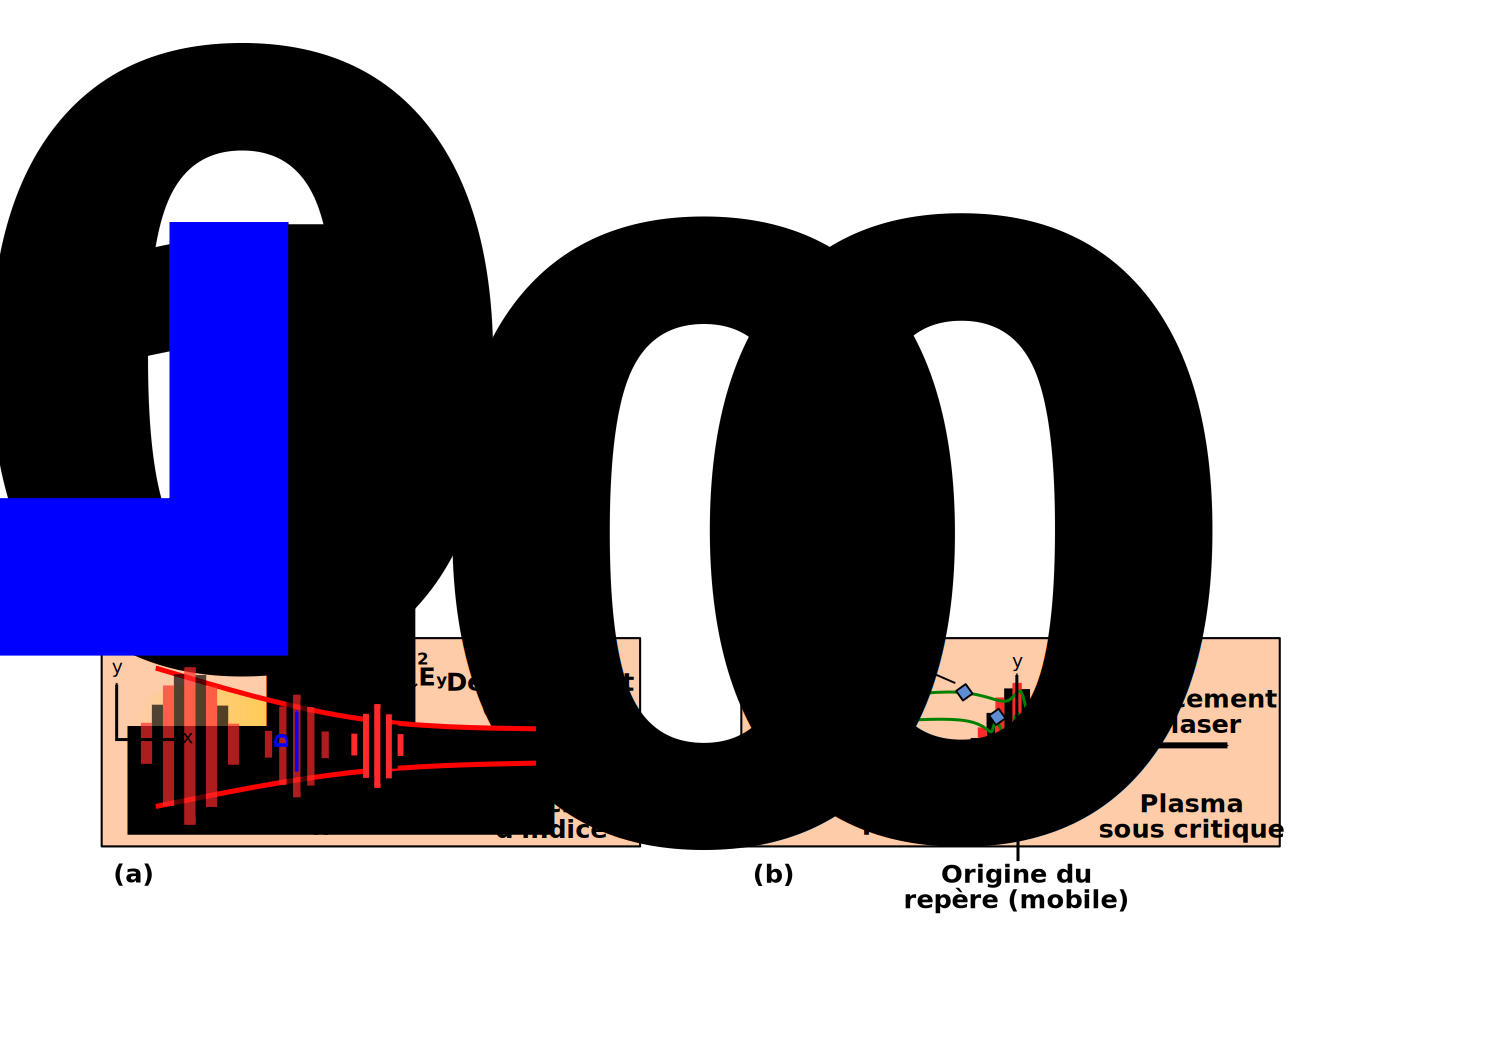
\includegraphics[width=\linewidth]{2-laser/interaction_laser_plasma.png}
    \caption{Illustration (a) de l'auto-focalisation relativiste et (b) de la force pondéromotrice dans un plasma sous-critique. Dans la figure (a) le laser se propage de gauche à droite dans un plasma sous-critique d'indice de réfraction $n_1$ alors que l'indice du plasma alentour est $n_0<n_1$. 
    Dans la figure (b) le repère est mobile et suit l'impulsion laser ; les particules défilent donc de droite à gauche dans la direction $-x$, et leur trajectoire est dessinée en vert. On 
    }
    \label{fig:2-interaction_laser_plasma}
\end{figure}

Ainsi, dans certaines conditions, une \textbf{zone de sous-densité électronique} peut donc être produite par le passage du laser. En particulier, un \textbf{canal sous-dense en électrons} peut être produit pour des intensités dépassant \parencite{gibbon_2013} : 
\begin{equation}
    I_0 > I_{canal} \approx 5.5\times 10^{19} ~ \dfrac{(D_L \si{[\um]})^2}{(\lambda_L \si{[\um]})^4} \dfrac{n_e}{n_c} ~ \si{[\W\per\cm^2]} ~ \rm .
    \label{eq:2-seuil_canal_ponderomoteur}
\end{equation}

Enfin, en plus des effets non-linéaires et relativistes présents pour des impulsions intenses d'extension spatiale limitée, des \textbf{effets de l'électrodynamique quantique en champ fort} peuvent aussi jouer un rôle important dès lors que la valeur du \textbf{paramètre quantique de l'électron} $\chi_e$ excède $\chi_e \gtrsim 0.1$ \parencite{zhang_2020}, avec \parencite{martinez_phd} :
\begin{equation}
    \chi_e = \dfrac{\gamma_e}{E_S} \sqrt{-\dfrac{\vec{E}_\parallel^2}{\gamma_e^2}+(\vec{E}_\perp + \vec{v} \times \vec{B})^2} ~ \rm ,
    \label{eq:2-chie_definition}
\end{equation}
où $E_S=m_e^2 c^3/e \hbar \approx 1.3 \times 10^{18} ~ \si{\V\per\m}$ est le champ de Sauter-Schwinger (aussi appelé simplement champ de Schwinger), qui est un champ caractéristique de l'électrodynamique quantique, et où $\vec{E}_\parallel$ et $\vec{E}_\perp$ sont respectivement les composantes parallèle et perpendiculaire du champ électrique par rapport à la vitesse $\vec{v}$ de l'électron. Ce paramètre est un invariant relativiste qui peut être compris comme étant le \textbf{champ électrique ressenti par la particule dans son référentiel propre}, normalisé à $E_S$ \parencite{dipiazza_2012}. Pour un électron relativiste oscillant dans une onde plane polarisée linéairement ($\gamma_e \sim \sqrt{1+a_0^2/2} \gg 1$ et $|\vec{E}_\perp+\vec{v} \times \vec{B}| \sim 2 \omega_L m_e c a_0/e$), on peut estimer que les effets de l'électrodynamique quantique doivent être considérés ($\chi_e \gtrsim 0.1$) dès lors que la valeur de $a_0$ est typiquement $a_0 \gtrsim 170$, ou encore $I_0 \gtrsim 4 \times 10^{22} ~ \si{\W \per \cm^2}$ (on a supposé une longueur d'onde de 1 µm). C'est aussi l'ordre de grandeur souvent considéré par les travaux théoriques pour inclure ces effets dans la description de \textbf{l'interaction laser-plasma} \parencite{dipiazza_2012, zhang_2020, capdessus_phd, martinez_phd}. 

Parmi les effets d'électrodynamique quantique en champ fort les plus notables (déjà évoqués au chapitre \ref{chap:1-particules}), nous pouvons mentionner la \textbf{production de paires électron-positron} par le processus Breit-Wheeler multi-photon ($\gamma + n \omega \to e^- + e^+$) et par le processus Trident multi-photon ($e + n \omega \to e + e^- + e^+$), ainsi que la \textbf{production de rayonnement énergétique} par le processus Compton inverse multi-photon ($e^- + n \omega \to e^- + \gamma$) \parencite{dipiazza_2012}. Pour ce type d'intensité laser, l'étude des mécanismes de rétroaction entre les effets d'électrodynamique en champ fort et la dynamique du plasma est un sujet de recherche très actif \parencite{zhang_2020, capdessus_phd}. 
Il est néanmoins intéressant de mentionner que l'influence de l'émission des photons sur la dynamique des électrons peut être modélisée d'un point de vue purement \textbf{classique} (force de friction) dès lors que la perte d'énergie des électrons peut être décrite de façon \textbf{continue} \parencite{burton_2014, niel_2018}. Des effets quantiques dans l'émission de rayonnement ont été mis en évidence par deux équipes en 2018 \parencite{poder_2018, cole_2018a} par la collision frontale d'un faisceau d'électrons d'énergie $>500 ~ \si{\MeV}$ avec un laser intense de $a_0 \gtrsim 10$. Cette configuration expérimentale permet en effet d'atteindre des valeurs de paramètre quantique $\chi_e$ significatives avec un laser d'intensité plus modérée (typiquement dès quelques $10^{21} ~ \si{\W\per\cm^2}$ pour un faisceau d'électrons d'énergie de l'ordre du $\si{\GeV}$ \parencite{vranic_2014}), et est à ce titre très étudiée dans le cadre d'études d'électrodynamique quantique en champ fort \parencite{vranic_2014, dipiazza_2012, zhang_2020}. 

Les différents régimes d'interaction laser-plasma évoqués jusqu'à présent sont résumés en figure \ref{fig:2-regimes_plasma}. L'axe des ordonnées indique l'intensité crête du laser considéré (de longueur d'onde 1 µm et de diamètre typique de tâche focale 10 µm), et l'axe des abscisses indique la densité électronique. Pour des intensités $\gtrsim 10^{18} ~ \si{\W \per \cm^2}$, les effets relativistes sont non négligeables $a_0 \gtrsim 1$, et deviennent de plus en plus importants à mesure que l'intensité augmente. Les effets d'électrodynamique quantique commencent aussi à être non négligeables dans l'interaction laser-plasma pour des intensités $\gtrsim 10^{22} ~ \si{\W \per \cm^2}$. Le seuil de transparence relativiste est indiqué par la ligne rouge, et est calculé via l'équation (\ref{eq:2-densite_critique_relativiste}). Les densités électroniques de quelques matériaux sont aussi indiquées à titre indicatif pour les conditions normales (ou ambiantes) de pression et de température (CNTP). La zone transparente au laser est indiquée par la zone 1. La force pondéromotrice y est toujours présente, et peut créer un canal sous-dense en électron en zones 1b et 1c (équation (\ref{eq:2-seuil_canal_ponderomoteur})). Le phénomène d'auto-focalisation relativiste est a priori significatif en zones 1c et 1d (équation (\ref{eq:2-seuil_auto-focalisation})). La zone 2 est opaque au rayonnement, et le laser pénètre seulement sur une épaisseur de peau. L'effet des collisions est d'autant plus important que la densité est importante, et que la température du plasma est faible, soit pour des intensités faibles. Les effets d'écrantage et d'oscillations plasma sont présents pour toutes les densités et intensités, ainsi que les phénomènes d'ionisation. D'autres processus non détaillés ici peuvent aussi intervenir dans l'interaction laser-plasma (voir figure \ref{fig:2-diversite_laser_fs}).

\begin{figure}[hbtp]
    \centering
    \includegraphics[width=0.8\linewidth]{2-laser/laser_plasma_zones.png}
    \caption{Résumé des différents régimes de propagation du laser dans l'interaction laser-plasma relativiste. En zone 1 le laser se propage dans le plasma, et peut créer un canal de sous-densité électronique en 1b et 1c, et être auto-focalisé en zones 1c et 1d. Il est réfléchi et pénètre seulement sur une épaisseur de peau en zone 2. Les paramètres quantifiant les effets de la relativité restreinte et de l'électrodynamique quantique (QED) sont aussi indiqués. Cette figure est disponible au format svg à l'adresse \url{github.com/lesnat/these} sous licence CC-BY et peut être librement adaptée.}
    \label{fig:2-regimes_plasma}
\end{figure}

En plus de ses effets sur la matière, l'interaction d'un laser intense avec un plasma peut aussi produire des particules énergétiques, en particulier des électrons et des photons $\gamma$.

\section{Production de particules énergétiques par laser}

Dans cette section, nous discuterons de l'utilisation de lasers intenses pour produire ou accélérer des particules de manière \textbf{directionnelle}, avec des énergies de \textbf{plusieurs MeV}.

Nous verrons en premier lieu comment utiliser astucieusement les propriétés des plasmas pour accélérer des \textbf{électrons}, en nous intéressant particulièrement aux processus d'accélérations dits d'\textit{accélération par sillage}, d'\textit{accélération directe} et d'\textit{accélération par $\vec{v} \times \vec{B}$}, respectivement importants dans les régimes sous-critiques, quasi-critiques et sur-critiques. D'autres mécanismes permettent néanmoins d'accélérer des électrons, ou de manière générale de transférer de l'énergie de l'impulsion laser au plasma, mais tous ne seront pas détaillés ici du fait de leur moins grande importance pour la suite de ce manuscrit. Certains de ces processus seront tout de même rapidement évoqués. De plus, nous ne discuterons ici que de l'accélération par un champ électromagnétique \textbf{laser}, et nous n'évoquerons donc pas les autres façons de produire des électrons énergétiques, tels que les méthodes utilisées dans les accélérateurs de particules, ou par la radioactivité $\beta^-$ par exemple.

Dans un second temps, nous verrons qu'en plus de leur potentiel pour l'accélération d'électrons, les lasers intenses constituent des candidats crédibles pour la production de \textbf{sources secondaires} tels que les \textbf{photons $\gamma$}. Nous verrons que ces lasers pourront être utilisés soit comme une source de \textbf{photons de basse énergie}, comme une source de \textbf{champ intense}, ou encore comme une façon de produire des \textbf{électrons énergétiques} qui seront ensuite utilisés pour la génération de particules secondaires. Nous présenterons enfin quatre schémas expérimentaux permettant de produire des sources de photons d'énergies autour du MeV par laser.


\subsection{Mécanismes d'accélération d'électrons}

Dans cette section, nous commencerons par étudier rapidement l'accélération par une onde plane d'un électron au repos dans le vide. Nous verrons notamment que, dans ces conditions, il n'est pas possible de lui transférer de l'énergie de manière permanente. Les sections suivantes présentent alors différentes méthodes permettant de contourner ce problème.

\subsubsection{Principe}

Pour comprendre l'interaction d'une onde électromagnétique avec des électrons dans un plasma, il peut être utile de commencer par considérer le cas théorique d'un seul électron dans le vide, interagissant avec une onde plane polarisée linéairement suivant $\vec{e}_y$ et se propageant dans la direction $\vec{e}_x$. Le potentiel vecteur de cette onde est : 
\begin{equation}
    \vec{A}(\xi)=A_0 \cos\left(\xi\right) ~ \vec{e}_y ~ \rm ,
\end{equation}
où $A_0$ est son amplitude maximale, et où $\xi=\dfrac{2 \pi}{\lambda_L} (x-ct)$ est sa phase. Pour un électron \textbf{initialement au repos à l'origine des positions}, on peut montrer \parencite{macchi_2012, yang_2011} que son impulsion est : 
\begin{equation}
    p_x=\dfrac{1}{4 m_e c} \left(\dfrac{e A_0}{c}\right)^2 \big[1+\cos(2 \xi)\big] ~ ; ~     p_y=\dfrac{e A_0}{c}\sin(\xi) ~ ; ~ p_z=0 \rm .
\end{equation}

Le déplacement de l'électron est alors contenu dans le plan $(\vec{e}_x,\vec{e}_y)$, et on peut remarquer que le \textbf{mouvement transverse} de l'électron est \textbf{oscillant à la même phase que l'onde}. Cette composante est directement proportionnelle à l'intensité du champ, et est donc significative sur le mouvement de l'électron (initialement au repos) \textbf{même pour des intensités faibles}. La composante \textbf{longitudinale} de l'impulsion de l'électron peut quant à elle être exprimée comme une \textbf{somme de deux termes} :
\begin{itemize}
    \item un terme proportionnel à $\cos(2 \xi)$ oscillant à \textbf{2 fois} la phase de l'onde, et 
    \item un terme $\dfrac{1}{4 m_e c} \left(\dfrac{e A_0}{c}\right)^2$ qui \textbf{ne dépend pas de la phase}, et correspond donc à un \textbf{mouvement de dérive constant} de l'électron dans la direction de $\vec{e}_x$.
\end{itemize}

Cette composante longitudinale est influencée seulement par le \textbf{champ magnétique} de l'onde, car la composante électrique de la force de Lorentz ne permet pas d'accélérer l'électron selon cette direction. Dans ce cas, l'impulsion \textbf{longitudinale} est proportionnelle au \textbf{carré} de l'amplitude de l'onde, et est donc \textbf{négligeable pour des intensités faibles} ($a_0\ll 1$, avec $a_0=e A_0/m_e c$), et \textbf{importante pour des intensités fortes} ($a_0 \gtrsim 1$). De plus, une fois que le mouvement de dérive a été initié, chaque phase accélératrice est suivie d'une phase décélératrice, et la \textbf{moyenne} du mouvement de l'électron sur \textbf{un cycle} donne donc au final un \textbf{gain d'énergie total nul}. 

Ce dernier aspect peut être généralisé, et est alors appelé \textbf{théorème de Lawson-Woodward}. Celui-ci stipule qu'il est impossible de transférer de l'énergie d'une onde plane à un électron dans le vide \textbf{de manière permanente} \parencite{esarey_2009, zaim_phd, gibbon_2013}, sous certaines hypothèses qui peuvent être résumées par \parencite{esarey_2009} :
\begin{enumerate}
\def\labelenumi{\arabic{enumi}.}
    \item la région d'interaction est supposée infinie,
    \item le laser se propage dans le vide sans murs ni bords,
    \item l'électron est ultra-relativiste dans la direction d'accélération,
    \item aucun champ électrique ou magnétique externe ne sont présents, et
    \item les effets non linéaires (force pondéromotrice, freinage par rayonnement, ...) sont négligés.
\end{enumerate}

Tout mécanisme d'accélération d'électrons par laser se devra alors d'\textbf{invalider au moins une de ces hypothèses} pour pouvoir produire un \textbf{gain net d'énergie} des électrons. 
Dans la suite, nous présenterons alors certains de ces mécanismes, même si nous ne rentrerons pas dans le détail de leur modélisation physique.

\subsubsection{Cible sous-critique et accélération par sillage}

Commençons tout d'abord par discuter de l'accélération d'électrons lors de la propagation d'un laser dans un plasma \textbf{sous-critique}, qui est très étudiée depuis la fin des années 1970 \parencite{tajima_1979}. Plusieurs régimes physiques d'accélération d'électrons ont été proposés (une revue est disponible en référence \parencite{esarey_2009}), mais nous discuterons ici particulièrement du mécanisme d'\textbf{accélération par sillage} (\textit{Laser Wakefield acceleration} en anglais), et principalement du \textbf{régime de la bulle} (\textit{blowout regime}). Celui-ci a été découvert théoriquement en 2002 \parencite{pukhov_2002} et a été mis en évidence expérimentalement 2 ans plus tard par trois équipes différentes \parencite{faure_2004, geddes_2004, mangles_2004}. Il est alors très étudié depuis, puisqu'il permet de produire des faisceaux d'électrons d'une \textbf{grande qualité} (par rapport aux autres modes d'accélération par laser), notamment de par leur \textbf{distribution en énergie très piquée}, avec une largeur de bande de typiquement quelques \%, et une \textbf{divergence angulaire faible}, typiquement quelques dixièmes de milliradians \parencite{esarey_2009}. De plus, l'\textbf{énergie} cinétique des électrons accélérés \textbf{peut être contrôlée} par un choix judicieux de paramètres laser-plasma, et atteindre des valeurs \textbf{de quelques MeV à plusieurs GeV} \parencite{faure_2019, leemans_2006, gonsalves_2019}. Enfin, le milieu utilisé pour l'accélération d'électrons étant typiquement un jet de gaz, la cible peut se renouveler continûment, permettant (en principe) de produire de tels faisceaux de particules avec un \textbf{haut taux de répétition}. Pour notre application, une de leurs limitations majeures par rapport à d'autres modes d'accélération concerne néanmoins la \textbf{charge totale du faisceau} d'électrons, qui est typiquement limitée à \textbf{quelques centaines de pico-Coulombs}. D'autres mécanismes d'accélération par laser dans un plasma sous dense peuvent quant à eux produire des faisceaux de quelques nanocoulombs, mais avec des propriétés nettement moins intéressantes en terme de dispersion angulaire et énergétique \parencite{esarey_2009}. 

Dans ce régime d'accélération, une impulsion laser d'\textbf{intensité relativiste} ($a_0 \gtrsim 1$) se propage dans un plasma \textbf{sous-critique}. Par l'intermédiaire de sa \textbf{force pondéromotrice}, elle peut éjecter les électrons sur son passage et créer une \textbf{cavité}, ou \textbf{bulle} quasiment \textbf{vide d'électrons} dans son sillage \parencite{pukhov_2002}. La \textbf{séparation de charge} produite induit ainsi un fort \textbf{champ électrique longitudinal}, qui peut \textbf{accélérer des électrons dans la direction de propagation du laser} si ceux-ci ont été convenablement injectés dans la cavité \parencite{pukhov_2002, esarey_2009}. Ce mécanisme est illustré schématiquement en figure \ref{fig:2-acceleration_sillage}. Les électrons les plus accélérés par ce champ sont alors ceux qui restent le plus longtemps \textbf{en phase} avec le champ accélérateur. Plusieurs mécanismes peuvent néanmoins limiter leur gain d'énergie maximal, que ce soit la diffraction de l'impulsion laser, le déphasage des électrons et du champ accélérateur, la perte d'énergie du laser au fur et à mesure de sa propagation, ou encore des instabilités laser-plasma \parencite{esarey_2009}.

\begin{figure}[hbtp]
    \centering
    \includegraphics[width=0.7\linewidth]{2-laser/acceleration_sillage_bulle.png}
    \caption{Illustration du mécanisme d'accélération par sillage dans le régime de la bulle. La force pondéromotrice de l'impulsion laser créé une cavité sous-dense en électrons dans son sillage, ce qui a pour effet de produire un champ électrique longitudinal. Les électrons injectés dans la cavité peuvent alors être accélérés dans la direction de propagation du laser.}
    \label{fig:2-acceleration_sillage}
\end{figure}

Pour créer une cavité sous dense en électrons de façon efficace, l'extension spatiale du laser doit être typiquement de l'ordre de grandeur de la longueur d'onde des oscillations plasma, et la force pondéromotrice doit pouvoir équilibrer le champ de rappel produit par le défaut de charges, ce qui peut se traduire par les conditions \parencite{esarey_2009, gordienko_2005} :
\begin{equation}
    c \tau_L \lesssim D_L ~ ; ~ \dfrac{\omega_{pe}}{c} D_L \sim \sqrt{a_0} ~ \rm .
    \label{eq:2-parametres_bulle}
\end{equation}

En pratique, les valeurs de $a_0$ considérées dans ce régime sont souvent de l'ordre de quelques unités \parencite{esarey_2009, faure_2019}. Les lasers de \textbf{haute puissance} (plusieurs centaines de TW) sont alors en pratique \textbf{peu focalisés} dans des matériaux \textbf{peu denses}, et, leur longueur de Rayleigh étant dans ce cas importante, ils peuvent \textbf{accélérer des électrons sur de grandes distances}, jusqu'à des \textbf{énergies très importantes} (par exemple jusqu'à 8 GeV pour un laser de 850 TW focalisé sur un diamètre de 70 µm pendant environ 20 cm à l'aide de capillaires \parencite{gonsalves_2019}). Au contraire, les lasers de \textbf{faible puissance} sont \textbf{plus focalisés} dans des matériaux plus \textbf{denses}, et accélèrent des particules \textbf{de plus faibles énergies sur de plus courtes distances} (par exemple un laser de 1 TW focalisé sur un diamètre de 2 µm pendant une distance 25 µm produit des électrons autour de 10 MeV \parencite{faure_2019}). Néanmoins, cette discussion qualitative ne résume pas la complexité du sujet, où la longueur d'accélération et la densité de la cible doivent aussi être choisis pour \textbf{optimiser la phase relative des électrons et de l'onde plasma}, et où l'injection des électrons dans la bulle constitue un enjeu de taille \parencite{esarey_2009}. 

Dans un cas satisfaisant les propriétés de l'équation \ref{eq:2-parametres_bulle}, il est possible d'estimer l'énergie cinétique $E_e^{bulle}$ des électrons accélérés, ainsi que leur nombre $N_e^{bulle}$ via \parencite{gordienko_2005} :
\begin{equation}
    E_e^{bulle} \si{[\MeV]}\sim ~ 1.1 ~ \dfrac{\tau_L \si{[\fs]}}{\lambda_L\si{[\um]}} \sqrt{P_0\si{[\TW]}} ~ ; ~ N_e^{bulle} \sim ~ 1.1 \times 10^9 ~ \lambda_L\si{[\um]} \sqrt{P_0\si{[\TW]}}\rm .
    \label{eq:2-scaling_Gordienko}
\end{equation}

Les énergies et nombres d'électrons typiquement atteignables par accélération par sillage dans le régime de la bulle sont alors tracés en figure \ref{fig:2-scaling_Gordienko}, pour les gammes de puissances et d'énergie pertinentes dans notre cas, et pour une longueur d'onde $\lambda_L=1 ~ \si{\um}$.

\begin{figure}[hbtp]
    \centering
    \includegraphics[width=0.7\linewidth]{2-laser/scaling_Gordienko.png}
    \caption{Estimations de l'énergie typique des électrons accélérés par sillage dans le régime de la bulle (graphique supérieur) ainsi que leur nombre (graphique inférieur), en fonction de la puissance laser. La charge totale est aussi indiquée en nanocoulombs (nC).}
    \label{fig:2-scaling_Gordienko}
\end{figure}

Comme évoqué précédemment, les énergies typiques sont de l'ordre de la centaine de MeV, et la charge totale du faisceau ne dépasse pas quelques nanocoulombs. Ces valeurs sont néanmoins seulement des \textbf{estimations}, et plusieurs techniques permettent de significativement modifier ce régime d'interaction. Il a par exemple été démontré que la génération d'énergies de l'ordre du \textbf{GeV} est possible avec seulement \textbf{40 TW} de puissance \parencite{leemans_2006} en utilisant des capillaires pour le guidage de l'impulsion sur de très longues distances. Au contraire, des expériences récentes ont démontré la production de faisceaux d'énergie autour du MeV, de \textbf{quelques pC} en focalisant une impulsion de quelques TW dans des jets de gaz denses de quelques 10 µm d'épaisseurs, mais avec un \textbf{taux de répétition de l'ordre du kHz} \parencite{faure_2019}. Les valeurs de charge totale données par ce modèle semblent aussi assez optimistes.

\subsubsection{Cible quasi-critique et accélération directe}

Comme nous l'avons vu précédemment, lorsqu'un laser interagit avec un plasma \textbf{sous-critique} il peut se propager sur des distances importantes, et ainsi accélérer des particules \textbf{en volume}. Pour le mécanisme d'accélération par sillage dans le régime de la bulle, l'impulsion laser doit rester suffisamment stable sur toute sa distance de propagation pour accélérer des particules de façon efficace, et une part non négligeable de son énergie n'est donc pas transférée aux particules.
Au contraire, pour un matériau de densité proche de la densité critique relativiste, appelé \textbf{quasi-critique}, le laser peut être significativement altéré lors de son interaction avec le plasma, et potentiellement y transférer une part plus importante de son énergie \parencite{gahn_1999a}. 
Parmi ces effets d'absorption, nous pouvons mentionner ici le mécanisme d'\textbf{accélération directe}, qui permet de produire \textbf{un nombre important} de particules (actuellement observé jusqu'à presque 100 nC de charge totale \parencite{ma_2018}) avec une \textbf{distribution en énergie large} pouvant atteindre \textbf{plusieurs centaines de MeV} \parencite{pukhov_1999}. 
Ce mécanisme a été décrit théoriquement dès la fin des années 1990 \parencite{pukhov_1999}, et il est notamment supposé jouer un rôle important pour l'accélération d'électrons dans les \textbf{long pré-plasma} lors de l'interaction laser-solide \parencite{pukhov_1999, krygier_2014}. 
Dans ce contexte, il est donc en compétition avec d'autres mécanismes d'accélération présents aux différentes densités du pré-plasma. Plusieurs expériences attribuent néanmoins des résultats de mesure à l'accélération directe dans des jets de gaz denses avec des durées d'impulsions de quelques centaines de fs \parencite{gahn_1999a, mangles_2005a}. Son étude est toujours active, par l'intermédiaire de modèles théoriques, de simulations numériques ou d'expériences \parencite{arefiev_2016, jirka_2020, krygier_2014, thevenet_2016}.

Comme nous l'avons vu précédemment, l'accélération d'électrons à partir d'une onde plane n'est pas possible \textbf{dans le vide}, car l'énergie gagnée par l'électron dans une phase accélératrice est ensuite perdue dans une phase décélératrice. 
Dans le mécanisme d'\textbf{accélération directe}, des \textbf{champs électromagnétiques externes} vont permettre à l'électron de \textbf{rester plus longtemps dans la phase accélératrice}, et ainsi pouvoir atteindre une énergie \textbf{plusieurs fois supérieures à l'énergie atteignable dans le vide} \parencite{arefiev_2016, jirka_2020, krygier_2014}.
En particulier, la présence d'un champ \textbf{transverse} à la direction de propagation du laser peut sous certaines conditions (fréquence du laser de l'ordre de la fréquence bétatron \parencite{corde_2013a}) faire osciller des électrons dans un mouvement appelé \textbf{bétatron} \parencite{pukhov_1999}, et ainsi \textbf{légèrement les déphaser} par rapport au champ laser ; leur permettant de rester en phase accélératrice plus longtemps que si ce champ transverse n'était pas présent.
En pratique, ces champs peuvent être produits directement par le laser, via le creusement d'un \textbf{canal sous-dense en électron} dans le plasma par la force pondéromotrice (voir section précédente). 
Cette \textbf{séparation de charges} produit en effet un champ électrique \textbf{transverse}, ainsi qu'un champ électrique longitudinal à l'interface vide-plasma \parencite{arefiev_2016}, et le courant d'électrons accélérés peut aussi induire un champ magnétique azimutal \parencite{jirka_2020, arefiev_2016}. L'effet croisé de ces champs induits et du champ laser peut alors rendre la trajectoire de l'électron très complexe, lui permettant parfois de rester en phase accélératrice pendant de longues distances, et parfois non.
Ce mécanisme d'accélération est ainsi extrêmement sensible aux conditions initiales d'injection des électrons \parencite{arefiev_2016, krygier_2014}.
Il est illustré très schématiquement en figure \ref{fig:2-acceleration_directe}, où la figure supérieure représente la trajectoire d'un électron accéléré par l'onde dans le vide, et la figure inférieure représente une trajectoire où l'effet global des champs a été bénéfique pour l'accélération, en déphasant l'électron par rapport à l'onde laser et lui permettant d'être accéléré plus longtemps.

\begin{figure}[hbtp]
    \centering
    \includegraphics[width=0.6\linewidth]{2-laser/acceleration_directe.png}
    \caption{Illustration du mécanisme d'accélération directe. En figure (a) l'électron a été accéléré dans le vide, sans gain d'énergie net après le passage du laser. En figure (b) la présence d'un champ électrique transverse créé par un canal sous-dense en électrons permet à l'électron de rester en phase accélératrice sur de longues distances, et donc d'acquérir une énergie cinétique importante.}
    \label{fig:2-acceleration_directe}
\end{figure}

Pour que ce mécanisme puisse avoir lieu dans un plasma quasi-critique homogène, la condition pour la production d'un canal sous dense en électrons par force pondéromotrice (équation (\ref{eq:2-seuil_canal_ponderomoteur})) doit être satisfaite, et il est aussi possible de montrer \parencite{arefiev_2016} que le seuil à partir duquel le phénomène de gain par oscillations bétatron transverses commence à devenir important est :
\begin{equation}
    G_{AD} =a_0 \sqrt{\dfrac{n_e}{n_c}} > 1 ~ \rm .
\end{equation}

Pour l'accélération directe ayant lieu dans \textbf{un pré-plasma de profil de densité exponentiel}, on peut approximer la forme de la distribution en énergie des électrons par une fonction exponentielle décroissante $f(E_e) \propto \exp(-E_e/T_e^{AD})$, avec $T_e^{AD}$ une énergie caractéristique souvent appelée \textit{température effective} qui peut être estimée comme \parencite{pukhov_1999} :
\begin{equation}
    T_e^{AD} \si{[\MeV]}\sim 1.5 \times 10^{-9} \sqrt{I_0 \si{[\W\per\cm^2]}} ~ \rm .
\end{equation}

Pour ce type de distributions en énergie, l'énergie totale contenue dans ces électrons est de l'ordre de $N_e^{AD} ~ T_e^{AD}$, et on peut donc estimer leur nombre total via :
\begin{equation}
    N_e^{AD} \sim 6.3 \times 10^{12} ~ \dfrac{\eta_{L \to e}^{AD} ~ E_L \si{[J]}}{T_e^{AD} \si{[MeV]}} ~ \rm ,
    \label{eq:2-acceleration_directe_nombre}
\end{equation}
où $\eta_{L \to e}^{AD}$ est l'efficacité d'absorption du laser dans ces électrons, qui peut varier de \textbf{quelques \%} si on considère seulement les électrons \textbf{éjectés}, à \textbf{plusieurs dizaines de \%} si on considère tous les électrons \textbf{accélérés} \parencite{pukhov_1999}. Des valeurs typiques de température effective et de nombre sont alors représentées en figure \ref{fig:2-scaling_acceleration_directe} en fonction de la puissance laser, où on a considéré une absorption de 30\%, une tache focale de largeur à mi-hauteur $10 ~ \si{\um}$ et une durée d'impulsion de largeur à mi-hauteur $30 ~ \si{\fs}$.

\begin{figure}[hbtp]
    \centering
    \includegraphics[width=0.7\linewidth]{2-laser/scaling_Pukhov.png}
    \caption{Estimations de la température effective et du nombre d'électrons accélérés par accélération directe dans un pré-plasma long, en fonction de la puissance laser.}
    \label{fig:2-scaling_acceleration_directe}
\end{figure}

Ces estimations montrent donc que ce type de situations permet d'atteindre des \textbf{températures effectives de plusieurs dizaines de MeV}, et des charges typiques de \textbf{dizaines de nanocoulombs} (jusqu'à 100 nC ont été observés et \textbf{attribués au mécanisme d'accélération directe} pour un laser de 200 TW, avec une durée d'interaction de l'ordre de 700 fs et 150J d'énergie laser \parencite{ma_2018}). Celles-ci reposent néanmoins sur des simplifications très importantes de la physique de l'interaction laser-plasma, qui peut s'avérer très complexe dans ce type de régimes, et ne doivent donc pas être prises comme des estimations trop quantitatives.

En effet, de nombreux autres mécanismes peuvent aussi entrer en jeu lors de l'interaction de ce type de laser avec un plasma de densité quasi-critique, tels que des instabilités paramétriques, qui permettent de transférer une part de l'énergie de l'onde laser à des ondes plasma. Ce type d'instabilités ne sera néanmoins pas présenté car sortant du cadre de cette thèse, mais plus d'informations sont disponibles notamment dans les références \parencite{moreau_phd, kruer_2003}. La fabrication de cibles de densité quasi-critique, permettant notamment d'étudier ce régime plus finement d'un point de vue expérimental, est aussi aujourd'hui un enjeu important \parencite{passoni_2020, prencipe_2017}.

\subsubsection{Cible sur-critique et accélération $\vec{v} \times \vec{B}$}

Pour des plasmas encore plus denses que ceux évoqués précédemment, la propagation du laser n'est plus possible. L'interaction d'un laser avec un matériau sur-critique (typiquement un solide ou un liquide) se fera alors non plus en volume mais seulement en \textbf{surface}, ou plus rigoureusement sur une profondeur limitée à l'épaisseur de peau. Les sources d'électrons produits par ce type d'interactions ont une \textbf{distribution en énergie large}, typiquement de forme \textbf{exponentielle décroissante} \parencite{malka_1996}, et une divergence angulaire de plusieurs dizaines de degrés de demi-angle \parencite{debayle_2010}. Ce type de régime d'interaction permet aussi de produire des \textbf{courants d'électrons très importants} à l'intérieur du solide \parencite{macchi_2012}. Nous discuterons ici en particulier du mécanisme d'accélération par la composante magnétique de la force de Lorentz, aussi noté $\vec{v} \times \vec{B}$ ou $\vec{J} \times \vec{B}$, qui peut être significatif dès lors que l'effet du champ magnétique devient important, i.e. pour des intensités relativistes $a_0 \gtrsim 1$. 

Comme nous avons pu le voir au début de cette section, lors de l'interaction d'une onde plane avec un électron initialement au repos dans le vide, ce dernier peut être accéléré notamment par la composante électrique du champ laser et acquérir une vitesse transverse à la direction de propagation de l'onde. Si le champ magnétique est suffisamment intense, le terme magnétique de la force de Lorentz peut faire osciller cet électron \textbf{longitudinalement}. L'énergie cinétique accumulée par cette particule lors de la phase accélératrice est néanmoins perdue lors d'une phase décélératrice. Dans le mécanisme d'accélération appelé $\vec{v} \times \vec{B}$, le laser se situe au niveau d'une \textbf{interface sur-critique}, et le mouvement d'\textbf{oscillation longitudinal} des électrons est alors \textbf{interrompu} lors du passage de l'interface sur-critique. Les électrons injectés dans la cible en ayant une vitesse longitudinale ne peuvent en effet plus être décélérés par l'onde électromagnétique, qui est évanescente derrière l'interface sur-critique, et ceux-ci conservent donc une part de l'énergie cinétique qu'ils ont acquise en phase accélératrice. Ce principe est illustré en figure \ref{fig:2-acceleration_magnetique}c. 
Dans l'interaction laser-solide, le nombre d'électrons injectés peut être très important (avec une densité de courant de l'ordre de $\sim e ~ n_c ~ c$ \parencite{macchi_2012}), ce qui créé une séparation de charges à l'interface sur-critique. Le champ électrostatique induit par cette séparation de charge a alors tendance à \textbf{freiner les électrons injectés} dans le matériau, jusqu'à pouvoir les arrêter totalement \parencite{macchi_2012}. En pratique, ce défaut de charges est \textbf{spontanément compensé} par un \textbf{courant de retour} d'électrons thermiques peu énergétiques, souvent appelés \textit{électrons froids}, qui a tendance à \textbf{neutraliser les charges et les courants} \parencite{macchi_2012, bell_1997}. 
Les électrons les plus énergétiques (chauds et suprathermiques) peuvent ainsi se propager dans le solide, en étant toutefois freinés par le champ électrostatique de séparation de charges \parencite{macchi_2012, bell_1997}.

\begin{figure}[hbtp]
    \centering
    \includegraphics[width=0.7\linewidth]{2-laser/acceleration_magnetique.png}
    \caption{Principe de l'accélération par $\vec{v} \times \vec{B}$. En (a) le laser accélère l'électron dans le plasma, qui acquiert une vitesse longitudinale par l'effet de la force magnétique. Il ne peut cependant pas obtenir de gain permanent en énergie car chaque phase accélératrice est suivie d'une phase décélératrice. En (b) une interface sur-critique permet à l'électron de conserver son énergie, car il est injecté dans la cible avant d'avoir pu être totalement décéléré.}
    \label{fig:2-acceleration_magnetique}
\end{figure}

De nombreuses expériences et simulations numériques tendent à montrer que la distribution en énergie des électrons accélérés dans l'interaction laser-solide est typiquement exponentielle décroissante, de \textit{température effective} \parencite{macchi_2012} :
\begin{equation}
    T_e^{\vec{v} \times \vec{B}} \sim \left(\sqrt{1+a_0^2/2}-1\right) m_ec^2 ~ \rm . 
\end{equation}

En utilisant un raisonnement similaire à celui qui a été mené pour dériver l'équation (\ref{eq:2-acceleration_directe_nombre}), on peut aussi estimer le nombre total d'électrons accélérés comme étant :
\begin{equation}
    N_e^{\vec{v} \times \vec{B}} \sim 6.3 \times 10^{12} ~ \dfrac{\eta_{L \to e}^{\vec{v} \times \vec{B}} ~  E_L \si{[J]}}{T_e^{\vec{v} \times \vec{B}} \si{[MeV]}} ~ \rm ,
\end{equation}
où $\eta_{L\to e}$ est une estimation de l'absorption du laser par les électrons, que l'on peut prendre de l'ordre de 10\% \parencite{price_1995, malka_1996}. Les énergies et nombres d'électrons typiques produits par ce mécanisme sont illustrés en figure \ref{fig:2-scaling_ponderomoteur}, où on a supposé une durée d'impulsion laser de largeur à mi-hauteur $30 ~ \si{\fs}$, une tache focale de largeur à mi-hauteur $10 ~ \si{\um}$ et une longueur d'onde de $1 ~ \si{\um}$. 
\begin{figure}[hbtp]
    \centering
    \includegraphics[width=0.7\linewidth]{2-laser/scaling_ponderomoteur.png}
    \caption{Estimations de la température effective et du nombre d'électrons accélérés par $\vec{v} \times \vec{B}$ ($\vec{v} \times \vec{B}$) dans l'interaction laser-solide, en fonction de la puissance laser. On a considéré une tache focale laser de largeur à mi-hauteur 10 µm.}
    \label{fig:2-scaling_ponderomoteur}
\end{figure}

On observe donc que la température effective est ici typiquement de \textbf{quelques MeV à quelques dizaines de MeV} et que la charge totale est de l'ordre de \textbf{quelques dizaines de nanocoulombs}, ce qui semble être en accord avec des données expérimentales typiques de l'interaction laser-solide \parencite{malka_1996, dubois_2014}. Ces estimations reposent néanmoins ici aussi sur des simplifications très importantes de la physique de l'interaction laser-plasma, et ne remplacent donc pas des études plus approfondies (notamment par l'intermédiaire de simulations numériques).

Dans l'interaction laser-solide, le mécanisme $\vec{v} \times \vec{B}$ peut aussi être en concurrence avec d'autres mécanismes d'accélération d'électrons, comme par exemple le chauffage stochastique \parencite{bourdier_2005, chopineau_2019}, ou l'effet Brunel pour un laser en incidence oblique en polarisation p \parencite{brunel_1987, chopineau_2019}. D'un point de vue expérimental, les propriétés des électrons injectés dans une cible solide ne peuvent pas être mesurées de manière directe, et doivent être déduites de mesures indirectes ou des propriétés des électrons éjectés de la cible, qui peuvent avoir été significativement affectées lors de leur propagation (par des collisions ou des champs électrostatiques par exemple) \parencite{link_2011a}.

\subsubsection{Comparaison des différents régimes d'accélération}

Comme nous avons pu le voir dans les sections précédentes, l'interaction laser-plasma dans le régime relativiste peut faire intervenir de nombreux processus (dont plusieurs n'ont pas été abordés ici, voir figure \ref{fig:2-diversite_laser_fs}), et la propagation du laser dans le plasma est fortement influencée par son intensité, son extension spatio-temporelle, et la densité et température des électrons du plasma notamment. De plus, les mécanismes d'accélération d'électrons par laser font souvent intervenir une \textbf{combinaison} de ces processus en synergie (ionisation, transparence relativiste, force pondéromotrice, ...). Ainsi, l'utilisation de \textbf{certains} paramètres laser (intensité, extension spatio-temporelle, contraste, ...) avec \textbf{certains} paramètres de cible (densité, matériau, géométrie, épaisseur, ...) va \textbf{fortement influencer} l'apparition des différents mécanismes d'accélération d'électrons, leur efficacité respective, et enfin les caractéristiques principales des sources d'électrons obtenues (charge, forme de la distribution en énergie, énergie caractéristique, distribution angulaire, ...). 
Par exemple, les conditions optimales pour l'\textbf{accélération par sillage dans le régime de la bulle} se situent à \textbf{intensité modérée et densité faible}, tandis que l'accélération par \textbf{$\vec{v} \times \vec{B}$} nécessite une \textbf{densité sur-critique}, et produit des particules d'autant plus énergétiques que l'\textbf{intensité du laser est élevée}. L'\textbf{accélération directe} peut être importante lorsque \textbf{l'intensité et la densité sont suffisantes} pour produire un canal sous-dense. Les différents régimes d'accélération d'électrons par laser sont illustrés en figure \ref{fig:2-regimes_electron}. Il est important de noter que cette figure suppose une longueur d'onde laser de 1 µm et une tache focale de 10 µm, et que ces zones peuvent donc être significativement différentes pour d'autres paramètres laser. La zone 1 indique les paramètres optimaux pour l'accélération par sillage dans le régime de la bulle, qui correspond ici à un laser d'environ 10 TW (en fixant la valeur de $a_0$ et de la taille de la tache focale on peut en déduire les autres paramètres). Les densités optimales peuvent ici grandement varier en fonction des choix de paramètres laser-plasma considérés (des exemples sont donnés dans la référence \parencite{faure_2019}). La zone 2 correspond au régime d'accélération directe, caractérisé par un gain important par rapport à l'accélération dans le vide, et une intensité suffisante pour la formation d'un canal sous-dense. La zone 3 correspond grossièrement à la zone quasi-critique, où la propagation du laser dans le plasma est fortement perturbée, et où de nombreux effets de couplage laser-plasma entrent en ligne de compte. Cette zone est aussi importante dans l'interaction laser-solide, de par l'expansion du solide à des densités quasi-critiques après son chauffage par l'impulsion principale ou par une pré-impulsion (contrôlée ou non). La zone 4 correspond à l'interaction laser-solide, ou laser-liquide. En particulier, dans la zone 4b les effets de la force magnétique sont importants, alors que l'accélération d'électrons dans la zone 4a nécessite de faire intervenir d'autres mécanismes, tels que l'effet Brunel pour une incidence oblique en polarisation p. Cette figure peut bien entendu être superposée à la figure \ref{fig:2-effets_plasma} afin d'estimer quels effets sont susceptibles d'interagir lors d'un choix d'intensité ou de densité de plasma considéré. 

\begin{figure}[hbtp]
    \centering
    \includegraphics[width=0.8\linewidth]{2-laser/laser_electron_zones.png}
    \caption{Régimes d'accélération d'électrons par laser pour différentes intensités et densités de plasma, en considérant un laser typique de longueur d'onde 1 µm focalisé sur un diamètre typique de 10 µm. En zone 1 on considère l'accélération par sillage dans le régime de la bulle, tandis que la zone 2 correspond aux paramètres typiques de l'accélération directe. La zone 3 permet de regrouper les nombreux effets pouvant avoir lieu à une densité quasi-critique. La zone 4 indique les régimes d'accélération par effet Brunel en 4a et par force magnétique en 4b. Dans ce cas la zone 4a s'étend au delà de la limite $a_0 \gtrsim1$ tandis que la zone 4b est limitée aux intensités relativistes $a_0 \gtrsim 1$.}
    \label{fig:2-regimes_electron}
\end{figure}

En pratique, il est aussi possible de choisir des schémas expérimentaux (géométries de cibles, intensité laser, ...) qui peuvent \textbf{combiner} différents régimes d'accélération. On peut par exemple citer l'utilisation en synergie des mécanismes d'accélération directe et d'accélération par sillage \parencite{zhang_2015b}, ou de l'accélération directe combinée à l'accélération par $\vec{v} \times \vec{B}$ par exemple \parencite{krygier_2014, pazzaglia_2020, jiang_2014}. Compte tenu de la physique très riche de ces régimes d'interaction, il est donc souvent nécessaire d'avoir recours à des \textbf{simulations numériques} pour pouvoir estimer les propriétés des sources d'électrons.

\subsection{Production de photons gamma par laser}

Dans cette section, nous discuterons particulièrement de différentes manières de produire des photons d'énergies multi-MeV par laser. Comme nous l'avons évoqué au début de ce chapitre, les lasers peuvent être à la fois vu comme une source de photons de basse énergie, ou comme une source de champ électromagnétique intense, et permettent de plus de produire des électrons énergétiques. Nous verrons que ces trois aspects pourront être mis à profits pour la production de photons de plusieurs MeV. Nous discuterons particulièrement ici des processus Compton inverse linéaire, Compton (ou Thomson) inverse multi-photon et Bremsstrahlung, tels que décrits dans le chapitre \ref{chap:1-particules}. Nous présenterons ici quatre configurations expérimentales spécifiques, que sont la collision frontale (ou contra-propagative) d'un faisceau d'électrons avec un laser peu intense (production de photons via le processus Compton inverse linéaire), la collision frontale d'un faisceau d'électrons avec un laser intense (production de photons via le processus Compton inverse multi-photon), la co-propagation d'un laser intense avec un faisceau d'électrons qu'il a lui même accéléré (production de photons via le processus Compton inverse multi-photon), et l'injection d'un faisceau d'électrons (qui peut avoir été produit par laser) dans un matériau solide appelé convertisseur (production de photons via le processus Bremsstrahlung). Ces diverses configurations sont illustrées en figure \ref{fig:2-config_gamma_laser}a, \ref{fig:2-config_gamma_laser}b, \ref{fig:2-config_gamma_laser}c et \ref{fig:2-config_gamma_laser}d, respectivement.

\begin{figure}[hbtp]
    \centering
    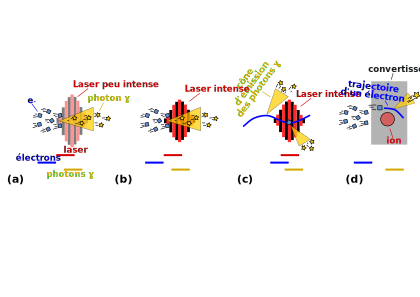
\includegraphics[width=\linewidth]{2-laser/config_gamma_laser.png}
    \caption{Illustrations de différents moyens de produire des photons $\gamma$ par laser, avec (a) l'émission de photons dans la collision frontale d'un faisceau d'électrons avec un laser peu intense (processus Compton inverse linéaire), (b) l'émission de photons dans la collision frontale d'un faisceau d'électrons avec un laser intense (processus Compton inverse multi-photon), (c) l'émission de photons par un électron accéléré dans la même direction que le laser (processus Compton inverse multi-photon), ou (d) l'émission de photons par la propagation d'un faisceau d'électrons dans un convertisseur (processus Bremsstrahlung). }
    \label{fig:2-config_gamma_laser}
\end{figure}

Nous donnerons quelques ordres de grandeurs typiques des caractéristiques des sources de photons produites par ce type de configuration, et nous intéresserons particulièrement à leur \textbf{brillance crête à 1 MeV} (ou par abus de langage plus simplement brillance à 1 MeV), exprimée en $\rm photons/s/mm^2/mrad^2/0.1\%BW$, où le terme $0.1\rm \%BW$ signifie 0.1\% de largeur de bande en énergie. Cette quantité permet en effet de prendre en compte les aspects les plus importants des sources pour notre type d'application, soit à la fois le \textbf{nombre de photons} d'énergie \textbf{autour du MeV}, mais aussi l'\textbf{extension spatio-temporelle} et la \textbf{divergence angulaire} de ceux-ci (ces aspects seront discutés plus en détail au chapitre \ref{chap:5-opti_theorique}).

\subsubsection{Laser contra-propagatif à un faisceau d'électrons : sources Compton inverse linéaire}

Dans le régime linéaire du processus Compton inverse, un électron diffuse de façon \textbf{inélastique} sur un photon de basse énergie, et peut lui transférer une part non négligeable de son énergie cinétique (voir chapitre \ref{chap:1-particules}). Dans ce cadre, les lasers peuvent ainsi fournir une densité importante de \textbf{photons de basse énergie} pouvant être diffusés par un faisceau d'électrons. Pour la collision frontale d'un faisceau d'électrons avec un laser peu intense, illustrée en figure \ref{fig:2-config_gamma_laser}a, l'énergie \textbf{maximale} des photons \textbf{diffusés} peut être calculée analytiquement et vaut \parencite{corde_2013a} :
\begin{equation}
    E_\gamma \si{[\MeV]} = 4 \times 10^{-6} ~ \gamma_e^2 ~ E_\omega \si{[\eV]}
\end{equation}

En considérant un laser diffusé de longueur d'onde $\lambda_L \sim 1$ µm, l'énergie initiale d'un photon est de l'ordre de $1$ eV, et pour produire des photons dans la gamme du MeV il est donc nécessaire de disposer d'une \textbf{source d'électrons} ayant une \textbf{énergie cinétique de l'ordre de 250 MeV} (facteur de Lorentz $\gamma_e \sim 500$).

En plus du laser \textit{diffusé}, il serait aussi a priori possible d'utiliser un laser \textit{accélérateur} pour produire la source d'électrons énergétiques. En supposant un laser accélérateur de longueur d'onde $0.8 ~ \si{\um}$ et de durée 30 fs (largeur à mi hauteur), l'accélération par sillage permettrait de produire des électrons de cette énergie en considérant une puissance laser de 40 TW, soit une énergie par impulsion de l'ordre de \textbf{seulement 1 Joule}, selon l'équation (\ref{eq:2-scaling_Gordienko}) et l'équation (\ref{eq:2-puissance_laser}). Pour cette puissance, l'équation (\ref{eq:2-scaling_Gordienko}) nous indique aussi que le nombre d'électrons accélérés est de l'ordre de $N_e \sim 5 \times 10^{9}$. 
En considérant une section efficace typique pour la diffusion Compton comme étant de l'ordre de $r_e^2 \sim 8 \times 10^{-26} ~ \si{\cm^2}$, le nombre de photons d'énergie de l'ordre du MeV pouvant être produits par ce type de dispositif dans une collision \textbf{frontale} est alors de l'ordre de \parencite{albert_2016, micieli_2016a} :
\begin{equation}
    N_\gamma \sim N_e N_{\omega} \dfrac{r_e^2}{\pi (D_s/2)^2} ~ \rm ,
\end{equation}
où $D_s$ est le diamètre typique des sources et $N_\omega$ est le nombre total de photons de basse énergie pouvant être diffusés. 

Pour un laser diffusé de longueur d'onde $0.8 ~ \si{\um}$ et d'énergie totale 0.5 J, le nombre de photons par impulsion est de l'ordre de $2 \times 10^{18}$, et en supposant un diamètre typique des sources de $20 ~ \si{\um}$ on obtient un nombre de photons produits dans la gamme du MeV de l'ordre de $2 \times 10^8$ photons. 

Cette estimation est supérieure d'un ordre de grandeur à des mesures effectuées pour des paramètres laser très proches (de l'ordre de $10^7$ photons mesurés) \parencite{chen_2013a}, et assez \textbf{typique} des sources combinant accélération d'électrons par sillage et diffusion Compton inverse linéaire \parencite{albert_2016}. Ces sources ont aussi une \textbf{dimension transverse} de \textbf{quelques µm à quelques dizaines de µm} \parencite{chen_2013a}, une durée de l'ordre de la durée des lasers accélérateurs et diffusés, soit ici \textbf{quelques dizaines de femtosecondes} \parencite{corde_2013a}, et une \textbf{divergence faible}, typiquement $<1^\circ$ \parencite{chen_2013a}. Ainsi, malgré leur \textbf{faible nombre de photons} ces sources présentent une \textbf{brillance crête à 1 MeV importante}, de l'ordre de $10^{19} \rm photons /s/mm^2/mrad^2/0.1\%BW$ pour la référence \parencite{chen_2013a}, voir jusqu'à plusieurs $10^{22} ~ \rm photons /s/mm^2/mrad^2/0.1\%BW$ pour la référence \parencite{yu_2016}. 

Compte tenu des faibles extensions spatio-temporelles à la fois du laser diffusé et du faisceau d'électrons, une des principales difficultés de ce type de méthodes concerne la \textbf{synchronisation et l'alignement} des particules incidentes \parencite{corde_2013a, albert_2016}. De plus, le \textbf{taux de conversion énergétique} y est \textbf{très faible}, de l'ordre de $10^{-12}$ \parencite{albert_2016}, et \textbf{deux impulsions lasers} sont nécessaires pour la production d'une seule source de photons $\gamma$. Sur ce dernier point, il est néanmoins intéressant de noter que des dispositifs expérimentaux ont été développés pour utiliser \textbf{la même impulsion laser} pour à la fois \textbf{accélérer les électrons} et \textbf{diffuser les photons}, soit en utilisant une \textbf{lame séparatrice} \parencite{chen_2013a}, soit \textbf{en faisant réfléchir le laser accélérateur sur un solide situé dans un jet de gaz}, lui permettant de \textbf{diffuser avec le faisceau d'électrons qu'il a lui même généré} \parencite{phuoc_2012}. Nous noterons de plus que le nombre de photons produits via une source d'électrons créée par accélérateur de particules est du même ordre de grandeur que ceux produits par laser, bien qu'en général d'énergies plus importantes \parencite{albert_2016}. Dans la gamme du MeV, les sources produites par laser sont néanmoins les sources Compton inverse linéaire avec la brillance la plus élevée actuellement \parencite{yu_2016}.

\subsubsection{Laser contra-propagatif à un faisceau d'électrons : sources Compton inverse multi-photon}

La production de rayonnement énergétique par collision électron-laser n'est cependant pas limitée au régime Compton linéaire, et en pratique le paramètre $a_0$ permet aussi d'estimer les \textbf{effets multi-photoniques} dans la diffusion de photons laser par des électrons énergétiques \parencite{corde_2013a, dipiazza_2012}. Ceci peut être compris d'un point de vue classique en remarquant que pour $a_0 \gtrsim 1$, la composante magnétique de la force de Lorentz joue un rôle important. Pour un électron initialement au repos oscillant dans une onde plane dans le vide, la trajectoire de l'électron n'est alors pas seulement transverse, mais possède aussi une composante longitudinale, et sa trajectoire dans le repère de sa vitesse moyenne suit une \textbf{figure en forme de 8} \parencite{yang_2011}. Pour $a_0 \gtrsim 1$, l'accélération de l'électron n'est alors constante ni en direction, ni en magnitude, car la composante magnétique de la force de Lorentz dépend de sa vitesse. Le rayonnement émis \textbf{classiquement} est donc caractérisé par \textbf{différentes fréquences}, émises à différentes harmoniques d'une fréquence fondamentale \parencite{lau_2003}. \textbf{D'un point de vue quantique}, cette émission de rayonnement à différentes harmoniques correspond alors à l'\textbf{absorption d'un nombre différent de photons lasers} pour chacune d'entre elles, et justifie ainsi l'appellation "multi-photon" pour ce processus \parencite{dipiazza_2012}. 

Dans ce régime d'émission, les photons diffusés peuvent donc avoir des énergies variées, et leur distribution en énergie est plus large que dans le régime linéaire. Suivant l'intensité du champ laser et l'énergie cinétique de l'électron, l'énergie des photons émis peut alors être soit \textbf{négligeable} soit \textbf{comparable} à l'énergie de l'électron. Ces deux cas sont appelés respectivement diffusion \textbf{Thomson} inverse multi-photonique, et diffusion \textbf{Compton} inverse multi-photonique. Plus précisément, la diffusion Thomson est définie telle que le \textbf{recul} de l'électron est \textbf{faible} dans son repère ($E_\gamma \ll m_e c^2$ dans le repère de l'électron), alors que la diffusion Compton est caractérisée par un recul \textbf{important de l'électron dans son repère} ($E_\gamma \gtrsim m_e c^2$). Le premier cas peut alors typiquement être traité à partir d'approximations \textbf{continues} et \textbf{classiques}, alors que le second doit être traité \textbf{en prenant en compte la nature discrète de l'émission}, soit autrement dit \textbf{d'un point de vue quantique}, tel qu'illustré de façon schématique en figure \ref{fig:2-regimes_diffusion}. En pratique, la transition entre une description théorique purement classique et un traitement purement quantique de la réaction au rayonnement est toutefois progressive, et dépend notamment de la valeur du paramètre quantique $\chi_e$ \parencite{burton_2014, dipiazza_2012, niel_2018}. D'un point de vue expérimental, le processus Compton inverse multi-photon a été observé pour la première fois dans une collision électron-laser au SLAC en 1996 \parencite{bula_1996}, avec des paramètres $a_0 \sim 0.6$ et $\chi_e \sim 0.3$, tandis que la réaction du faisceau d'électrons au rayonnement émis a quant à elle été mesurée pour la première fois sur le laser Gemini en 2018, où une signature quantique de la réaction au rayonnement semble avoir été observée \parencite{cole_2018a, poder_2018}.

\begin{figure}[hbtp]
    \centering
    \includegraphics[width=0.7\linewidth]{2-laser/diffusion_electron-laser.png}
    \caption{Terminologie des différents régimes de diffusion électron-photon dans un champ laser, pour un électron relativiste contra-propagatif à un laser.}
    \label{fig:2-regimes_diffusion}
\end{figure}

Lorsque l'on considère un laser intense (typiquement $a_0>10$ \parencite{corde_2013a}), le régime \textbf{non linéaire}, ou \textbf{multi-photon} du processus Compton inverse peut donc devenir significatif. Pour la discussion suivante, nous utiliserons des estimations initialement calculées pour le régime \textbf{Thomson non-linéaire} \parencite{corde_2013a}, soit pour des énergies de photons émis $E_\gamma \ll m_e c^2$ dans le repère de l'électron. Pour des discussions d'ordre de grandeur, nous supposerons que ces estimations restent valides pour des photons émis avec une énergie de quelques MeV dans le référentiel du laboratoire. Lorsque ceci est possible, nous prendrons soin de comparer ces estimations avec des données expérimentales disponibles. 

Dans le régime Thomson non linéaire, pour un électron \textbf{contra-propagatif} à une \textbf{onde plane} polarisée linéairement (voir figure \ref{fig:2-config_gamma_laser}c), l'énergie caractéristique des photons est donnée par \parencite{corde_2013a} :
\begin{equation}
    E_\gamma \si{[\MeV]} \sim 3.74 \times 10^{-6} ~ \dfrac{\gamma_e^2 a_0}{\lambda_L \si{[\um]}} ~ \rm ,
\end{equation}
et le nombre de photons émis par électron est de l'ordre de \parencite{corde_2013a} :
\begin{equation}
    N_\gamma \sim 2 \times 10^{-2} a_0 \dfrac{\tau_L \si{[\fs]}}{\lambda_L \si{[\um]}} ~ \rm .
\end{equation}

Pour un laser diffusé de paramètres $a_0  \sim 10$, et $\lambda_L=1$ µm, la production de photons d'énergie $>$ MeV nécessite ici des électrons d'énergies de l'ordre de $\sim 80$ MeV. En considérant une source d'électrons accélérés par sillage, le nombre d'électrons correspondant (via l'équation \ref{eq:2-scaling_Gordienko}) est $N_e \sim 2 \times 10^{9}$ pour un laser accélérateur de durée 30 fs et de longueur d'onde 1 µm. Le nombre total de photons énergétiques peut alors être estimé comme étant de l'ordre de $N_\gamma \sim 10^{9}$, pour un laser diffusé de durée 30 fs. 
Des \textbf{expériences} avec des paramètres relativement proches (énergie des électrons autour de 500 MeV et $a_0 \sim 2$ pour le laser diffusé) rapportent de l'ordre de $10^{7}$ photons émis par $10^8$ électrons incidents, avec des énergies de l'ordre de la dizaine de MeV \parencite{sarri_2014}. La brillance à 6 MeV de ces sources y est estimée autour de $10^{19} ~ \rm photons /s/mm^2/mrad^2/0.1\%BW$, ce qui en faisait selon ces auteur$\cdot$es la source de photons multi-MeV la plus brillante jamais rapportée dans la littérature à cette date (en 2014). 
Les estimations précédentes sont cohérentes en terme de nombre de photons avec l'expérience (autour de $10^8$ photons d'énergie 5 MeV pour les paramètres indiqués dans l'article). Une revue des sources de ce type avant 2013 est aussi disponible en référence \parencite{corde_2013a}.

\textbf{Dans ces gammes d'énergies et d'intensités}, et pour un faisceau d'électron contra-propagatif au laser, le régime Compton inverse multi-photon présente alors a priori des propriétés \textbf{similaires} au régime Compton inverse linéaire en terme de \textbf{nombre} et d'\textbf{énergies} de photons. Ce régime d'interaction nécessite cependant des énergies d'électrons moins importantes, mais produit une source de photons avec un spectre large \parencite{corde_2013a, sarri_2014}. D'un point de vue expérimental, ce schéma présente les mêmes difficultés que les sources Compton inverse linéaire, notamment au niveau de l'alignement et de la synchronisation du laser et du faisceau d'électrons. 
Les mêmes solutions ont alors été envisagées, et le schéma initialement développé par \cite{phuoc_2012} suscite un intérêt certain depuis quelques années. Plusieurs études \textbf{numériques} \parencite{huang_2019,long_2019,ong_2019,jirka_2020b} suggèrent en effet qu'il serait possible de produire des sources de photons multi-MeV par le processus Compton inverse multi-photon en utilisant \textbf{un seul} laser qui accélère des électrons dans une cible sous-critique (jet de gaz ou mousse quasi-critique) et est réfléchi par un matériau sur-critique avant de collisionner avec les électrons qu'il a lui même accélérés. Ce principe a déjà été réalisé avec succès expérimentalement avec un jet de gaz pour le régime Compton inverse linéaire \parencite{phuoc_2012, yu_2016}. D'après les auteur$\cdot$es de ces études, celui-ci permettrait de produire des sources de brillance à 1 MeV allant jusqu'à $10^{22} \rm photons /s/mm^2/mrad^2/0.1\%BW$ avec des lasers de caractéristiques \textbf{déjà disponibles}, soit quelques $10^{21} ~ \si{\W \per \cm^2}$ d'intensité, focalisés sur quelques µm pendant quelques dizaines de fs \parencite{huang_2018, huang_2019}. En particulier, l'utilisation de mousses quasi-critiques permettrait \textbf{d'auto-focaliser} le laser, et ainsi d'atteindre des intensités plus importantes \textbf{au point de collision} \parencite{huang_2019}. L'efficacité de ce schéma semble augmenter avec l'intensité du laser, et des simulations Particle-In-Cell 2D et 3D indiquent qu'il permettrait d'atteindre plus de 1\% de conversion d'énergie laser dans les photons d'énergie $>1$ MeV pour $I_0 \gtrsim 4 \times 10^{21} ~ \si{\W \per \cm^2}$ \parencite{huang_2018}. Ces résultats sont prometteurs, mais nécessitent néanmoins d'être confirmés par des expériences. Comme évoqué précédemment, la collision frontale de faisceaux d'électrons avec un laser intense est aussi d'un grand intérêt pour des études d'électrodynamique en champ fort, et celles-ci considèrent souvent des faisceaux d'électrons d'énergies dans la gamme du GeV collisionnant frontalement avec des lasers de paramètre $a_0$ de quelques dizaines à quelques centaines \parencite{bula_1996, poder_2018, cole_2018a, dipiazza_2012, zhang_2020, vranic_2014}. 

\subsubsection{Laser co-propagatif à un faisceau d'électrons : sources Compton inverse multi-photon}

Considérons maintenant une configuration différente, où un électron \textbf{initialement au repos} émet des photons $\gamma$ par le processus Compton inverse multi-photon en interagissant avec un laser intense (figure \ref{fig:2-config_gamma_laser}). Si on modélise le laser par une onde plane en polarisation circulaire, et telle que $a_0 \gg 1$, on peut monter que l'énergie maximale des photons est \parencite{corde_2013a}:
\begin{equation}
    E_\gamma \si{[\MeV]} \sim 3\times 10^{-7} ~  \dfrac{a_0^3}{\lambda_L\si{[\um]}}
\end{equation}
tandis que le nombre de photons émis à l'énergie moyenne \textbf{par électron et par période d'oscillation} (de longueur $\lambda_{osc}$) est de l'ordre de \parencite{corde_2013a} :
\begin{equation}
    N_\gamma \sim 5 \times 10^{-2} a_0 ~ ; \lambda_{osc} \sim  \dfrac{a_0^2}{4} \lambda_L \rm .
\end{equation}

Ainsi, il est possible de produire des photons d'énergie autour du MeV pour des valeurs de $a_0 \gtrsim 180$, qui est l'ordre de grandeur attendu pour les installations laser les plus intenses actuellement en cours de lancement (Apollon, Aton, …). Le \textbf{nombre de photons émis} peut dans ce cas être \textbf{comparable} voire supérieur au \textbf{nombre d'électrons accélérés}. En considérant un laser de 10 PW et $a_0=200$ avec l'estimation (\ref{eq:2-scaling_Gordienko}), on peut par exemple estimer le nombre de photons produit \textbf{par cycle} lors de la propagation d'un tel laser dans une cible sous-critique comme étant de l'ordre de $\sim 10^{12}$, où un cycle correspond à une propagation de l'ordre du cm \parencite{corde_2013a}. Ces photons étant produits par l'accélération d'électrons dans le champ du laser, l'extension spatio-temporelle typique de la source de photons peut être rapidement estimée comme étant de l'ordre de grandeur des dimensions de l'impulsion laser. Ce type de situation permettrait alors de produire des sources de \textbf{très haute brillance}, car comprenant de nombreux photons très localisés spatio-temporellement. Ces estimations ont toutefois été obtenues pour un cas théorique d'oscillation d'électrons dans le vide via un laser de polarisation circulaire, pour le régime Thomson, et où les effets du \textbf{freinage de l'électron par émission de rayonnement} ont été \textbf{négligés}. Comme nous l'avons vu précédemment, ces régimes se situent néanmoins typiquement dans les gammes d'intensités où le freinage par rayonnement commence à devenir \textbf{important}. Ce type d'estimations semble toutefois indiquer que ce régime d'interaction peut être \textbf{très prometteur} pour la production de sources de \textbf{haute brillance}, avec un taux de répétition de l'ordre du tir par minute. Pour ces régimes d'intensité, des \textbf{simulations numériques} Particle-In-Cell 3D semblent indiquer que, pour des lasers polarisés linéairement comme circulairement, les propriétés des sources de photons sont principalement influencées par le régime de propagation de l'impulsion (plasma transparent ou opaque au laser) \parencite{ji_2014}. En particulier, le taux d'absorption dans les photons et la collimation de ces sources sont bien meilleures pour des cibles transparentes d'un point de vue relativiste, et peuvent atteindre plus de 10\% d'absorption et une divergence typique de l'ordre de 20 à 30 degrés pour une cible homogène de densité électronique $30 ~ \rm n_c$, et pour $a_0 \gtrsim 400$ \parencite{ji_2014}. 
Néanmoins, pour des cibles transparentes d'un point de vue relativiste mais de densité $> \rm n_c$, des simulations semblent indiquer que la propagation de l'impulsion laser dans le plasma peut devenir instable et changer de direction ; modifiant par la même occasion la direction d'émission des photons \parencite{stark_2016,huang_2017a}. Une configuration a alors été proposée, consistant en un \textbf{canal transparent d'un point de vue relativiste inséré dans une matrice opaque pour le laser} \parencite{stark_2016}. Pour un canal de la taille typique du laser, ce type de schéma permet alors de guider l'impulsion sur une plus grande distance, et les champs magnétiques produits influencent positivement la production massive ($> 10^{12}$) et localisée (inférieure aux dimensions de l'impulsion laser) de photons multi-MeV relativement collimatés (typiquement 20 degrés) \parencite{stark_2016, long_2019, huang_2017a}. Cette configuration, bien que prometteuse, nécessite néanmoins des lasers d'intensités typiques $I_0 \gtrsim 5 \times 10^{22} ~ \si{\W \per \cm^2}$, et n'a pas encore été étudiée expérimentalement. L'alignement de la tâche focale de quelques µm avec un canal de même dimensions présente ici aussi un défi expérimental, et impliquera possiblement une variation des propriétés des sources importante entre chaque tir, suivant l'alignement du laser avec le canal.

\subsubsection{Faisceau d'électrons se propageant dans la matière : sources Bremsstrahlung}

Enfin, des \textbf{électrons accélérés par laser} peuvent aussi produire du rayonnement en étant \textbf{déviés au voisinage de noyaux dans la matière}, comme représenté en figure \ref{fig:2-config_gamma_laser}d et tel que nous l'avons décrit au chapitre \ref{chap:1-particules}.
La production de ce type de sources de photons dans la gamme du MeV par laser a d'ailleurs été \textbf{démontrée expérimentalement} dans l'interaction laser-solide \textbf{dès les années 1990} \parencite{kmetec_1992, perry_1999a, norreys_1999}, et au début des années 2000 pour des sources d'électrons produites dans des jets de gaz \parencite{edwards_2002}.

En considérant un électron incident d'énergie $E_e$, le nombre de photons d'énergie supérieure à $E_\gamma^{min}$ peut être estimé comme \parencite{carron_2007} :
\begin{equation}
    N_\gamma(E_\gamma>E_\gamma^{min}) \sim N_e ~ \rho ~ L \dfrac{S_m^{rad}(E_e)}{E_e} \left[\ln\left(\dfrac{E_e}{E_\gamma^{min}}\right) - \left(1-\dfrac{E_\gamma^{min}}{E_e}\right)\right] ~ \rm ,
\end{equation}
avec $S_m^{rad}(E_e)$ le pouvoir d'arrêt radiatif massique d'un électron d'énergie $E_e$, $\rho$ la densité du matériau et $L$ l'épaisseur du convertisseur. Ainsi, pour un faisceau de $7 \times 10^9$ électrons d'énergie autour de $18 ~ \si{\MeV}$ injecté dans un convertisseur de tantale ($Z=73$) d'épaisseur $L \sim 2~ \si{\mm}$, le nombre de photons produit avec une énergie $E_\gamma>8 ~ \si{\MeV}$ est estimé comme étant de l'ordre de $8 \times 10^9$, ce qui est supérieur d'un ordre de grandeur au nombre de photons mesuré pour ces paramètres (de l'ordre de $3 \times 10^8$ \parencite{giulietti_2008}).

Pour un électron incident relativiste, l'énergie moyenne $<E_\gamma>$ et l'angle d'émission moyen $<\theta_\gamma>$ des photons produits peuvent aussi être rapidement estimés via \parencite{carron_2007} :
\begin{equation}
    <E_\gamma> \sim \dfrac{E_e}{2} \dfrac{\left(1-\dfrac{E_\gamma^{min}}{E_e}\right)^2}{\ln\left(\dfrac{E_e}{E_\gamma^{min}}\right)-\left(1-\dfrac{E_\gamma^{min}}{E_e}\right)} ~ ; ~
    <\theta_\gamma> \sim \dfrac{m_e c^2}{E_e + m_e c^2} ~ \rm .
    \label{eq:2-energie_angle_Brem}
\end{equation}

Ainsi, en ne considérant que les électrons d'énergie $>m_e c^2$, la production de photons d'énergie moyenne autour du MeV nécessite des électrons de seulement $2.5 ~ \si{\MeV}$. Cette énergie est alors \textbf{bien moins importante} que celles nécessaires pour les sources Compton inverse linéaire ou Compton inverse multi-photon, et \textbf{peut être facilement produite par des lasers actuels} d'intensités $I_0 \gtrsim 10^{18} ~ \si{\W \per\cm^2}$. Il a par ailleurs été montré numériquement que, pour l'interaction d'un laser d'intensité $I_0=10^{22} ~ \si{\W\per\cm^2}$ avec une cible solide en cuivre, la production de photons par le processus Bremsstrahlung est dominante sur le rayonnement émis par Compton inverse multi-photon dès lors que l'épaisseur de la cible dépasse quelques µm \parencite{martinez_2020}. L'angle moyen d'émission de ces photons est aussi directement lié à l'énergie de l'électron incident, et est de l'ordre de $20$ degrés pour un électron d'énergie $E_e \sim 1 ~ \si{\MeV}$, ou $1$ degré pour un électron d'énergie $E_e \sim 30 ~ \si{\MeV}$ d'après l'équation (\ref{eq:2-energie_angle_Brem}). Cette estimation ne prend néanmoins pas en compte la diffusion des électrons dans la matière.

Les sources obtenues par \textbf{jet de gaz} semblent être \textbf{plus collimatées que les sources produites par interaction laser-solide} \parencite{edwards_2002, albert_2016}, et leur \textbf{taille caractéristique} est typiquement \textbf{de l'ordre de la centaine de micromètres} \parencite{ben-ismail_2011, glinec_2005} et augmente avec l'épaisseur du convertisseur considéré \parencite{ben-ismail_2011}.
Pour un laser d'énergie 1 J de durée 50 fs, il a été montré expérimentalement que les sources d'électrons produites par un jet de gaz dense permettent d'atteindre des énergies de plusieurs MeV avec une distribution large et avec une charge totale de l'ordre du nanocoulomb, en considérant un régime d'accélération différent du régime de la bulle \parencite{oishi_2011}. Une étude numérique menée par ces auteur$\cdot$es a aussi permis de montrer que le nombre de photons d'énergie $>0.5 ~ \si{\MeV}$ émis par Bremsstrahlung dans un convertisseur millimétrique en tungstène ($Z=74$) est 20 fois supérieur en utilisant cette source d'électrons produite dans un jet de gaz, par rapport à une source d'électrons produite par le même laser via une cible solide en cuivre d'épaisseur $30 ~ \si{\um}$ \parencite{oishi_2011}. 
Pour des \textbf{lasers d'énergies dans la gamme d'une centaine de Joules}, les sources produites par interaction laser-solide permettent quant à elles d'atteindre des \textbf{taux de conversion énergétiques de l'ordre de plusieurs $\%$} \parencite{henderson_2014, palaniyappan_2019} (soit un nombre de photons par tir $>10^{11}$ \parencite{palaniyappan_2019}), avec des \textbf{divergences typiques de l'ordre de $10$ à $30$ degrés} \parencite{henderson_2014, palaniyappan_2019} et une \textbf{taille de source de l'ordre de la centaine de µm} \parencite{palaniyappan_2019}. Pour un laser de cette gamme d'énergie, il a aussi été montré \textbf{expérimentalement} que les sources d'électrons produites dans des \textbf{mousses quasi-critique} de quelques centaines de micromètres d'épaisseur et injectées dans un convertisseur centimétrique en fer permettent d'\textbf{augmenter la dose produite par les photons d'un facteur $10^3$} par rapport à une source d'électrons produite avec le même laser et une \textbf{cible solide fine} en cuivre \parencite{rosmej_2019a}.

\subsubsection{Comparaison des différents modes de productions de photons}

Nous avons vu que la production de photons $\gamma$ dans la gamme du MeV peut reposer sur trois processus (Compton inverse linéaire, Compton inverse multi-photon et Bremsstrahlung) et sur quatre schémas de principe expérimentaux (voir figure \ref{fig:2-config_gamma_laser}). Les intensités nécessaires à la production de ce type de sources de photons sont résumées en figure \ref{fig:2-regimes_gamma}. Les zones 1a et 1b correspondent à la collision d'un laser avec un faisceau d'électrons, supposé de charge maximale 1 nC concentrée dans un volume de $(10 \si{\um})^3$. Le régime Compton inverse linéaire peut être dominant en zone 1a, alors que le processus Compton inverse multi-photon est dominant en zone 1b, pour $a_0>1$. Pour des valeurs d'intensité typiquement $\gtrsim 10^{22} ~ \si{\W\per\cm^2}$, le processus Compton (ou Thomson) inverse multi-photon peut devenir significatif dans l'interaction laser-plasma pour la production de photons dans la gamme du MeV. Les zones 2a, 2b et 2c correspondent alors respectivement à la production de rayonnement dans un plasma sous-critique \parencite{brady_2012}, quasi-critique \parencite{brady_2013} et sur-critique \parencite{ridgers_2012}. La zone 3 correspond quant à elle à la production de photons par le processus Bremsstrahlung dans l'interaction laser-solide, et est plus efficace pour des numéros atomiques élevés et des énergies importantes pour les électrons incidents.

\begin{figure}[hbtp]
    \centering
    \includegraphics[width=0.8\linewidth]{2-laser/laser_gamma_zones.png}
    \caption{Illustrations de différents régimes de production de photons $\gamma$ d'énergies autour du MeV par laser, où en 1a et 1b le laser collisionne avec un faisceau d'électrons (pouvant avoir été produit par laser), en 2a, 2b et 2c le laser interagit avec un matériau respectivement sous-critique, quasi-critique et sur-critique, et en 3 des électrons (pouvant avoir été produits par laser) sont injectés dans un convertisseur solide.}
    \label{fig:2-regimes_gamma}
\end{figure}

\newpage
\printbibliography[heading=subbibintoc]
\end{refsection}

\part{Méthodes}
\chapter{Considérations expérimentales}
\label{chap:3-methodes_exp}
\minitoc
\begin{refsection}
\newpage
\fbox{\begin{minipage}{\textwidth}
    \textbf{Contexte :}\\
    Le processus Breit-Wheeler multi-photon a été observé en laboratoire au SLAC en 1997, où de l'ordre de $200$ positrons ont été détectés en $20 ~ 000$ tirs, avec un taux de répétition de l'ordre du Hertz. Le processus Breit-Wheeler linéaire n'a quant à lui jamais été directement observé en laboratoire depuis sa prédiction en 1934 (chapitre \ref{chap:1-particules}), même si plusieurs schémas de principe d'expériences ont été proposés depuis 2014. 
    
    \medskip
    \textbf{Résumé du chapitre :}\\
    Dans ce chapitre, les propositions publiées avant fin 2020 sont présentées. Celles-ci font toujours intervenir des photons d'énergie $\gtrsim \si{\MeV}$ produits par les processus Compton inverse linéaire, Compton inverse multi-photon, ou Bremsstrahlung. Ces sources peuvent alors collisionner ensemble, ou avec des photons de plus basse énergies produits par d'autres mécanismes (tableau \ref{fig:3-tableau_propositions}). Dans le cadre de cette thèse, nous nous concentrerons principalement sur les sources de photons produits par Bremsstrahlung, avec un taux de répétition de l'ordre du Hertz (d'autres possibilités seront néanmoins évoquées dans les chapitres suivants). Le schéma de principe d'une cible multi-couches permettant d'atteindre cet objectif est ensuite présenté (figure \ref{fig:3-principe_cibles}), ainsi que la stratégie de détection des positrons élaborée au CELIA conjointement à cette thèse. Ce nouveau concept de détection est basé sur le comptage d'un faible nombre de positrons dans un environnement bruité (figure \ref{fig:3-principe_comptage}). En accord avec cette stratégie de détection, nous nous fixons pour objectif de pouvoir produire de l'ordre de quelques positrons via le processus Breit-Wheeler linéaire par tir laser.
    
    \medskip    
    \textbf{Informations complémentaires :}\\
    Plus d'informations sur les différents schémas de principe d'expériences pour l'observation du processus BWL sont disponibles dans les références indiquées dans le tableau \ref{fig:3-propositions_BWL}. Une revue des problématiques liées à l'utilisation de cibles à taux de répétition important est aussi disponible dans \parencite{prencipe_2017}.
\end{minipage}}
\newpage


\section{Principe de l'expérience}

Dans cette section, nous discuterons de différents schémas de principes expérimentaux proposés pour produire et détecter des positrons créés par collision de photons.
Les résultats obtenus par \cite{burke_1997} lors de l'expérience ayant permis la détection du processus Breit-Wheeler \textbf{multi-photon} seront très rapidement présentés, et serons suivis d'une discussion sur les différentes propositions expérimentales élaborées pour la détection du processus Breit-Wheeler \textbf{linéaire} en laboratoire. Nous verrons alors que celles-ci font appel à des stratégies très variées, et que cette thématique est très actuelle. 

\subsection{Détection du processus Breit-Wheeler multiphoton au SLAC}

Bien que le processus Breit-Wheeler \textbf{linéaire} n'ait jamais été observé pour le moment en laboratoire (voir chapitre \ref{chap:1-particules}), le processus Breit-Wheeler \textbf{multi-photon} à quant à lui \textbf{déjà été détecté} en 1997 au Stanford Linear Accelerator Center par \cite{burke_1997}.

Dans cette expérience, un faisceau de $7 \times 10^9$ électrons de $46.6 ~ \rm GeV$ collisionnait avec un laser \textit{Nd:verre} doublé en fréquence, de longueur d'onde $527 ~ \rm nm$ (photons d'énergie $2.35 ~ \rm eV$), d'énergie totale $650 ~ \rm mJ$, et d'intensité $1.3 \times 10^{18} ~ \rm W/cm^2$ ($a_0 = 0.36$) pour créer des photons $\gamma$ d'énergie allant jusqu'à $29.2 ~ \rm GeV$ via le processus Compton inverse. Les photons énergétiques ainsi produits pouvaient à leur tour collisionner avec le même laser pour produire des paires $e^-e^+$ par le processus Breit-Wheeler multi-photon ($\gamma + n \omega \to e^- e^+$, avec $n \omega$ un nombre $n$ de photons laser), comme représenté sur la figure \ref{fig:3-Burke}a. La conservation de l'énergie implique dans ce cas qu'un minimum de $4$ photons laser ait été nécessaire pour créer une paire $e^-e^+$ (la collision à deux photons nécessitant un photon de haute énergie de plus de $111 ~ \rm GeV$, voir chapitre \ref{chap:1-particules}). Dans cette expérience, les positrons produits avec une énergie cinétique $<20 ~ \rm GeV$ étaient ensuite défléchis par un champ magnétique et détectés par un calorimètre, noté \textit{PCAL} sur la figure \ref{fig:3-Burke}a.

\begin{figure}[hbtp]
	\centering
	\includegraphics[width=\linewidth]{3-experience/experience_BWM.png}
	\caption{Résumé de l'expérience de \cite{burke_1997} avec (a) le schéma de principe de l'expérience, et (b) le nombre de positron mesurés en fonction du paramètre $a_0$ du laser (noté ici $\eta$). La zone grisée représente ici le bruit de fond, avec un intervalle de 95\% de confiance. Figures tirées de la référence \parencite{burke_1997}.}
	\label{fig:3-Burke}
\end{figure}

Après analyse du calorimètre, $175 \pm 13$ positrons ont été détectés en $21962$ tirs lasers, dont $106 \pm 14$ ne peuvent pas être expliqués par le bruit systématique (zone grisée sur la figure \ref{fig:3-Burke}b). Ces positrons mesurés sont attribués au processus Breit-Wheeler multi-photon, car le bruit de fond et les autres processus connus (notamment le processus Trident multi-photon, voir chapitre \ref{chap:1-particules}) ne permettent pas d'expliquer ce comportement. On peut noter que le \textbf{nombre de positrons détectés par tir est de l'ordre de $10^{-2}$ à $10^{-1}$}, avec un \textbf{taux de répétition de l'ordre du tir par seconde} ($0.5 ~ \rm Hz$).

\subsection{Propositions de schémas expérimentaux pour la détection du processus Breit-Wheeler linéaire}

En 2014, soit presque 20 ans après les résultats obtenus par \parencite{burke_1997}, une expérience qui pourrait permettre de mesurer le processus Breit-Wheeler \textbf{linéaire} en laboratoire (création de paires $e^-e^+$ par la collision de deux photons réels) a été imaginée par O. J. Pike, E. G. Hill et S. J. Rose et F. Mackenroth \parencite{pike_2014}.
Cette proposition, illustrée en figure \ref{fig:3-propositions_BWL}a, ne fait intervenir \textbf{que des lasers} comme sources d'énergie, et implique de faire collisionner un \textbf{faisceau directionnel} de quelques $10^8$ photons autour du $\rm GeV$ avec une \textbf{source X thermique} de température de quelques centaines d'$\rm eV$. La source de haute énergie serait créée en accélérant des électrons par le processus d'\textbf{accélération par sillage}, puis en injectant ce faisceau d'électron dans une feuille d'or pour convertir leur énergie cinétique en photons $\gamma$ par \textbf{rayonnement de freinage} (Bremsstrahlung). La source X serait quant à elle créée par un laser énergétique éclairant un hohlraum (cavité en or) de longueur centimétrique. D'après les premières estimations, la température de la source X semble être d'une très grande importance, et les auteur$\cdot$es estiment qu'en utilisant des lasers actuels de type \textit{Ti:Sa} de quelques $\sim 100 ~ \rm TW$ de puissance pour produire la source de haute énergie, combiné avec un laser de type NIF ou LMJ (énergie de plusieurs centaines de kilo-joules) pour la source X, il serait possible de produire \textbf{jusqu'à $10^2$ à $10^5$ positrons par tir}, selon le nombre et l'énergie des $\gamma$ de haute énergie ainsi que de la température du hohlraum. L'interaction de photons de plusieurs $\rm MeV$ avec la feuille d'or ou avec le hohlraum pourrait néanmoins aussi produire des positrons par le processus Bethe-Heitler ($\gamma Z \to Z e^- e^+$), ce qui compliquerait l'interprétation des mesures.

En 2016, l'utilisation deux sources de photons directionnelles et de plus basse énergie a ensuite été suggérée par X. Ribeyre, E. D’Humières, O. Jansen, S. Jequier, V. T. Tikhonchuk et M. Lobet \parencite{ribeyre_2016}.
Ces auteur$\cdot$es discutent particulièrement de l'opportunité d'utiliser des sources $\gamma$ \textbf{identiques}, à \textbf{haut taux de répétition} (comparé au NIF/LMJ) et d'\textbf{énergie autour du MeV}. Le schéma de principe de cette expérience est illustré en figure \ref{fig:3-propositions_BWL}b. Après avoir discuté de plusieurs possibilités pour la production de telles sources, un modèle théorique et une revue de la littérature leur permis d'établir que les sources \textbf{Bremsstrahlung} et \textbf{Compton inverse multi-photon} seraient les sources les plus crédibles pour ce schéma expérimental. En particulier, des sources Bremsstrahlung \textbf{déjà produites en laboratoire} permettraient selon ce modèle de créer \textbf{de l'ordre de $10^4$ paires BWL par tir}, en considérant la collision de deux sources de photons $\gamma$ produites chacune par un laser de $100 ~ \rm J$ d'énergie. Ce type de sources produit néanmoins de manière inhérente un nombre très important de positrons dans la matière (jusqu'à $10^{10}$, soit de plusieurs ordres de grandeurs supérieur au nombre de paires BWL), pouvant constituer un bruit de mesure pour la détection des positrons BWL. Des sources de photons $\gamma$ produites par \textbf{Compton inverse multi-photon} dans une feuille d'aluminium ou un jet de gaz dense permettraient quant à elles de créer un nombre de paires BWL \textbf{équivalent aux sources Bremsstrahlung} ($\sim 10^4$) avec un \textbf{bruit de positrons plus faible} (entre $10^7$ et $10^9$ d'après les premières estimations), en considérant un laser de 150 J et d'intensité $I_0=10^{23} ~ \rm W/cm^2$. Comme les deux sources de photons sont relativement directionnelles (avec un demi-angle de divergence de $15$ à $30$ degrés typiquement), l'\textbf{angle de collision} moyen entre les sources est aussi un \textbf{paramètre libre} pour l'expérience. Choisir un angle de collision proche de $90$ degrés pourrait alors permettre d'orienter préférentiellement les positrons dans la direction de la bissectrice des deux faisceaux, par un effet cinématique, et ainsi potentiellement faciliter leur détection. Cette possibilité a été étudiée plus en détail pour des collisions de faisceaux de photons mono-énergétiques dans deux articles publiés les années suivantes \parencite{ribeyre_2017, ribeyre_2018}.


En 2017, une étude préliminaire faisant intervenir deux sources \textbf{Compton inverse linéaire}, \textbf{identiques} et \textbf{directionnelles}, produites par le \textbf{couplage de deux lasers avec un collisionneur d'électrons} (ou un collisionneur à électrons-positrons) a été publiée par I. Drebot, L. Serafini, D. Micieli, E. Tassi, E. Milotti et V. Petrillo \parencite{drebot_2017a}.
L'idée d'un collisionneur de photons réels basé sur la diffusion Compton inverse linéaire de lasers dans un collisionneur de leptons n'est néanmoins pas nouvelle, et a été étudiée théoriquement depuis les années 1980 sans jamais être concrètement réalisée. Ce principe est néanmoins toujours discuté actuellement, pour l'étude de collisions de photons de quelques MeV à plusieurs centaines de GeV \parencite{chou_2018, takahashi_2019}. Ce type de schéma expérimental, illustré en figure \ref{fig:3-propositions_BWL}c, permettrait alors non seulement d'étudier le processus Breit-Wheeler linéaire mais aussi la \textbf{diffusion photon-photon}, dont la section efficace est bien plus faible mais est maximisée pour une énergie du centre de masse autour du MeV \parencite{drebot_2017a}. Dans leur proposition, ces auteur$\cdot$es considèrent deux faisceaux d'électrons de $260 ~ \rm MeV$ et $250 ~ \rm pC$ couplés avec deux lasers d'énergie $2 ~ \rm J$, soit des caractéristiques proches de la source de photons $\gamma$ développée pour le projet ELI-NP \parencite{tanaka_2020}. Des \textbf{simulations numériques} prenant en compte les différents processus en présence (processus de collisions photon-photon, mais aussi électron-photon et électron-électron) permettent alors d'estimer le \textbf{nombre d'évènements par tir} comme étant \textbf{de l'ordre de $10^{-4}$}, soit de l'ordre de \textbf{plusieurs dizaines de paires électron-positron détectées par heure} en considérant un taux de répétition de $100 ~ \rm Hz$. Selon ces auteur$\cdot$es, ce type de schéma expérimental pourrait permettre d'étudier le processus Breit-Wheeler linéaire en profondeur (notamment ses effets de polarisation), et représente un défi technique qui leur semble néanmoins raisonnable. D'autres propositions existent pour la détection en laboratoire du processus de diffusion photon-photon réel dans la région du $\rm MeV$, et celles-ci pourraient aussi permettre l'observation du processus Breit-Wheeler linéaire (qui a une section efficace beaucoup plus importante), mais dans la mesure ou cet objectif n'est pas explicitement indiqué, ces propositions ne sont pas détaillées ici (voir les références \parencite{homma_2016, takahashi_2018, takahashi_2019}).


En 2019, la production de paires par collision de \textbf{faisceaux de photons directionnels et identiques} produits \textbf{par laser} via le processus \textbf{Compton inverse multi-photon} fut aussi étudiée par J. Q. Yu,  R. H. Hu,  Z. Gong,  W. J. Ma, C. E. Chen, H. Y. Lu , T. Takahashi, Y. S. Huang et X. Q. Yan \parencite{yu_2019}.
Ces sources de photons énergétiques seraient produites par la propagation de lasers de $10 ~ \rm PW$, du type de ceux de l'installation ELI-NP \parencite{tanaka_2020}, se propageant à l'intérieur de tubes micrométriques vides situés à l'intérieur d'une feuille d'or de quelques centaines de micromètres d'épaisseur. Ce type de source, ayant été préalablement étudiées par l'intermédiaire de simulations PIC 2D \parencite{yu_2019}, seraient à la fois \textbf{très directionnelles} (divergence $<3$ degrés) et \textbf{très intenses} (nombre de photons d'énergie $>10 ~ \rm keV$ de l'ordre de $10^{14}$). Leur collision, illustré en figure \ref{fig:3-propositions_BWL}d, permettrait alors de produire \textbf{jusqu'à $10^8$ paires par tir}, en considérant une distance de collision de $70 ~ \rm \mu m$ et un angle de collision de $170$ degrés entre les deux sources. Le grand nombre de paires BWL produites permettrait alors, selon ces auteur$\cdot$es, de détecter ces positrons en un seul tir avec un rapport signal sur bruit suffisant, et ce en considérant une distance de collision jusqu'à presque $2 ~ \rm mm$, grâce à la faible divergence de ces sources. De plus, le bruit produit par les processus concurrents (Bethe-Heitler, Triplet, ...) serait assez limité dans le tube vide et le nombre de positrons de bruit n’excéderait pas quelques $10^7$. Ces deux derniers aspects ont néanmoins été critiqués et commentés par \cite{wang_2020a} qui \textbf{mettent en doute l'hypothèse des ions immobiles} utilisée dans ces simulations PIC 2D. Ceux-ci montrent qu'en considérant des ions mobiles, la divergence des sources augmente fortement (de l'ordre de $22$ degrés), et le \textbf{nombre de paires BWL produites diminue} d'un facteur $10$ pour une distance de collision de $200 ~ \rm \mu m$. Le \textbf{bruit de positrons} produits par d'autres processus tendrait aussi à \textbf{augmenter}, de part l'interaction de particules énergétiques avec des ions ayant migré dans le tube initialement vide.


Un schéma expérimental très similaire fut aussi étudié par O. Jansen, T. Wang, T. J. Stark, T. Toncian, A. V. Arefiev,  Z. Gong, et D. Stutman dans deux articles distincts, en collaboration avec X. Ribeyre et E. d'Humières précédemment évoqués \parencite{jansen_2018a, wang_2020}. Dans ces références, la collision de deux sources identiques produites par le processus \textbf{Compton inverse multi-photon} est considérée pour des \textbf{lasers plusieurs PW} se propageant dans une \textbf{cible structurée}, composée d'un canal de densité de l'ordre de $10 ~ \rm n_c$ (avec $\rm n_c$ la densité critique) inséré dans une matrice de densité solide (de l'ordre de $100 ~ \rm n_c$ dans les simulations). Le principe de ce type de sources, initialement étudié par \cite{stark_2016}, est illustré en figure \ref{fig:3-propositions_BWL}e, et le schéma de la collision est similaire à la figure \ref{fig:3-propositions_BWL}b. Avec ce type de cibles, et par le biais de simulations 2D \parencite{jansen_2018a} ou 3D \parencite{wang_2020}, ces auteur$\cdot$es estiment qu'ils serait possible de produire \textbf{de l'ordre de $10^4$ paires par tir} à une distance de collision de $250 ~ \rm \mu m$, avec un angle de collision de $90$ degrés. Des estimations ont aussi été menées en considérant un schéma similaire à celui proposé par \cite{pike_2014} et illustré en figure \ref{fig:3-propositions_BWL}a, où la source de photons Bremsstrahlung est remplacée par la source Compton inverse multi-photon précédemment évoquée. Le nombre maximal de paires produites par ce type de schéma serait alors de l'ordre de $10^{5}$ par tir pour un hohlraum centimétrique de température $400 ~ \rm eV$, de l'ordre de $800$ pour une température de 200 eV et seulement 2 paires pour une température de 100 eV. Les auteur$\cdot$es Y. He, T. G. Blackburn en collaboration avec T. Toncian et A. V. Arefiev ont aussi proposé d'utiliser ce type de cible pour effectuer la collision de photons \textbf{à l'intérieur du canal} sous dense, en tirant simultanément avec deux lasers de quelques $10^{22} ~ \si{\W\per\cm^2}$ d'intensité de chaque côté du canal \parencite{he_2020}. Il est alors montré que le nombre de paires produites par le processus BWL peut atteindre \textbf{plusieurs $10^8$ paires par tir} et est très supérieur au nombre de paires produites par le processus Breit-Wheeler multi-photon. Les paires produites seraient alors\textbf{ collimatées dans l'axe de propagation laser}, et pourraient être accélérées à des énergies cinétiques supérieures à $200 ~ \si{\MeV}$. 

Enfin, une dernière proposition en date de fin 2020 fut une étude menée par A. Golub, S. Villalba-Chavez, H. Ruhl et C. Müller \parencite{golub_2020}. Ces auteur$\cdot$es y discutent de la possibilité de faire collisionner un f\textbf{aisceaux de photons de l'ordre du GeV}, produits par \textbf{Bremsstrahlung} via des \textbf{électrons accélérés par sillage}, avec un \textbf{laser à rayons X} (XFEL, pour \textit{X-ray Free Electron Laser}). Le schéma de principe de cette expérience est illustrée en figure \ref{fig:3-propositions_BWL}f. Un modèle analytique leur permet d'estimer l'énergie optimale de la source d'électrons, ainsi que l'épaisseur optimale du convertisseur permettant de maximiser la production de paires BWL. Sous ces conditions optimales, et avec un laser à rayons X d'énergies $0.3 ~ \rm keV$, il est estimé qu'il serait possible de produire \textbf{jusqu'à $350$ paires par tir}, en faisant collisionner les deux faisceaux à une distance de $40 ~ \rm cm$. Les électrons et positrons émis par BWL seraient alors préférentiellement orientés dans la direction du faisceau de photons Bremsstrahlung, avec une énergie autour de $600 ~ \rm MeV$. La propagation de particules énergétiques dans la matière constitue néanmoins ici aussi une source de bruit de positrons importante. Cette proposition serait en principe réalisable sur les installations du projet HiBEF \parencite{hibef}.

\begin{figure}[hbtp]
	\centering
	\includegraphics[width=\linewidth]{3-experience/experiences_BWL.png}
	\caption{Illustrations des propositions expérimentales pour l'observation de la création de paires par collision de photons réels, avec (a) la proposition de \cite{pike_2014} faisant intervenir une source Bremsstrahlung avec une source X thermique, (b) la proposition de \cite{ribeyre_2016} faisant intervenir deux sources Bremsstrahlung ou Compton inverse multi-photon, (c) la proposition de \cite{drebot_2017} faisant intervenir deux sources Compton inverse linéaire, (d) la proposition de \cite{yu_2019} faisant intervenir deux sources Compton inverse multi-photon, (e) une illustration du principe des sources initialement proposées par \cite{stark_2016} et appliquées à la production de paires BWL dans \cite{jansen_2018a} et \cite{wang_2020}, et (f) la proposition de \cite{golub_2020} faisant intervenir une source Bremsstrahlung et un laser à rayons X (XFEL). Les figures proviennent respectivement des références \parencite{pike_2014}, \parencite{ribeyre_2016}, \parencite{drebot_2017a}, \parencite{yu_2019}, \parencite{wang_2020} et \parencite{golub_2020}.}
	\label{fig:3-propositions_BWL}
\end{figure}

\subsection{Résumé des propositions}

Comme nous pouvons le constater sur la figure \ref{fig:3-propositions_BWL}, les approches actuellement envisagées pour l'observation du processus BWL peuvent être assez diverses. Certaines considèrent la collision d'un faisceau directionnel de photons d'énergies dans la gamme du $\rm GeV$ avec un rayonnement relativement peu directionnel et peu énergétique dans la gamme de la centaine d'$\rm eV$, telles que les propositions de \cite{pike_2014} et l'étude de \cite{wang_2020}. D'autres proposent au contraire de faire collisionner deux faisceaux de photons identiques, directionnels, et d'énergies autour du $\rm MeV$, telles que les propositions de \cite{ribeyre_2016}, \cite{drebot_2017}, \cite{yu_2019},  \cite{wang_2020} et \cite{he_2020}. Une autre possibilité est l'utilisation de deux faisceaux directionnels mais d'énergies très différentes, l'un dans la gamme du $\rm GeV$ et l'autre dans la gamme du $\rm keV$, telle que la proposition de \cite{golub_2020}. Ces différentes approches sont résumées en figure \ref{fig:3-tableau_propositions}. Nous rappelons que le seuil de création de paires est donné par la condition $E_{CM} = \sqrt{2 E_1 E_2 (1-\cos{\psi_{12}})}>2 m_e c^2$, où $E_1$, $E_2$ est l'énergie du photon 1, 2 respectivement, et $\psi_{12}$ est l'angle de collision entre les photons.

\begin{figure}[t]
	\centering
	\includegraphics[width=\linewidth]{3-experience/tableau_experiences.png}
	\caption{Résumé des propositions expérimentales pour sur la création de paires par BWL, en début 2021. XFEL signifie X-ray free electron laser, CIL signifie Compton inverse linéaire, Brem signifie Bremsstrahlung, et CIM signifie Compton inverse multi-photon. La collision de deux sources dans le régime keV (de quelques 100 eV à quelques 10 keV) ne permet pas de produire des paires car l'énergie de la collision est trop faible. Ces sources peuvent néanmoins produire des paires BWL en collisionnant avec des photons dans la gamme du GeV (entre 100 MeV et quelques GeV). La collision de deux sources d'énergies dans le régime du MeV (entre 100 keV et 100 MeV) est aussi possible. Le coin supérieur droit du tableau est symétrique par rapport à la diagonale.}
	\label{fig:3-tableau_propositions}
\end{figure}

Dans ces différentes stratégies, le nombre de paires produites par tir et le taux de répétition sont aussi très variables, allant d'un nombre de paires de $10^{-4}$ par tir avec un taux de répétition de $100 ~ \rm Hz$ pour \cite{drebot_2017} à un nombre de paires de $10^5$ par tir mais avec un nombre de tirs très faible (limité par la cadence des grosses installations NIF/LMJ) pour \cite{pike_2014}. Le nombre de positrons produits par d'autres processus dans la zone d'interaction est aussi très différent, pouvant être inférieur à la production de paires par BWL pour \cite{drebot_2017} à très largement supérieur au nombre de paires produites par BWL, pour les propositions faisant intervenir des sources Bremsstrahlung telles que les propositions de \cite{pike_2014}, \cite{ribeyre_2016}, ou \cite{golub_2020}. Les sources de photons produites par Compton inverse multi-photon ont aussi pour le moment seulement été étudiées via des simulations numériques, alors que des sources Bremsstrahlung sont produites par laser en laboratoire depuis les années 1990 (voir chapitre \ref{chap:2-laser}). Enfin, certaines propositions nécessitent l'adaptation d'installations existantes telle que la proposition de \cite{drebot_2017}, et certaines seront possibles sur des lasers actuellement en construction, comme les propositions de sources Compton inverse multi-photon de \cite{ribeyre_2016}, \cite{yu_2019}, \cite{wang_2020}, \cite{he_2020} alors que d'autres pourraient a priori être effectuées sur des installations déjà disponibles, comme les sources Bremsstrahlung de \cite{pike_2014}, \cite{ribeyre_2016} ou \cite{golub_2020}. 

Dans le cadre de cette thèse, nous nous concentrerons principalement sur l'étude de \textbf{sources de photons identiques, directionnelles, dans la gamme du MeV}, telles que proposées dans \cite{ribeyre_2016}. Pour des sources crées par les processus Bremsstrahlung ou Compton inverse multi-photon, le \textbf{nombre de positrons produits par BWL} sera \textbf{faible devant le bruit de positrons créés par d'autres processus}. 
D'autres particules énergétiques (électrons, photons, ...) ou des ondes électromagnétiques produites lors de l'interaction laser-plasma pourraient aussi interagir avec et perturber l'appareil de mesure. Pour pouvoir attribuer un signal mesuré à la détection du processus BWL, il sera donc nécessaire de \textbf{filtrer} et de \textbf{bien caractériser} le \textbf{bruit de mesure}.

\section{Cadre de cette thèse}

Dans cette section, nous évoquerons rapidement certaines possibilités de production et la détection de positrons créés par le processus BWL, en considérant des \textbf{lasers de caractéristiques déjà disponibles}.

Nous verrons dans un premier temps que les sources Bremsstrahlung semblent être des candidates crédibles pour la production de photons $\gamma$ avec un taux de répétition de l'ordre du $\rm Hz$. Nous discuterons ensuite d'un schéma de principe de cibles qui pourrait être utilisé pour produire de telles sources de photons. Les développements théoriques et numériques présentés dans la suite de ce manuscrit sont néanmoins adaptés ou adaptables à d'autres processus de production de photons.

Nous discuterons enfin de la stratégie développée conjointement à cette thèse, principalement par J.-L. Dubois et D. Khaghani, pour la détection des positrons produits par le processus BWL. Cette stratégie de détection nous permettra de nous fixer un \textbf{objectif réaliste de production de paire} via le processus BWL, qui sera de l'ordre de \textbf{quelques paires BWL par tir}.

\subsection{Stratégies pour la production de photons gamma}

%chap 2 = 4 types de setup (résumé avantages et inconvénients). Ici : Brem car le + simple dans un premier temps avec des lasers d'énergies modérées (gamme du Joule) (+ haut taux de rep ?). On peux avoir plusieurs modes d'accélération d'électrons (cibles sous-critique, quasi-critique et sur-critique). Ici : on choisit des cibles solides car charge du faisceau d'électron plus importante, et des lasers présentant deux faisceaux courte focale sont d'ores et déjà disponibles (+ autres justif ? cible en un seul bloc ?). Malgré leur plus faible charge, l'utilisation de cibles gazeuses pourraient néanmoins s'avérer pertinentes, en particulier grâce à leur plus faibles divergences ainsi que la possibilité de les utiliser à haut taux de répétition. Nous pouvons combiner quasi-critique + sur-critique (ref exemple et appel figure). De plus, nous nous restreindrons à l'étude de l'incidence normale afin de limiter le nombre de paramètres à faire varier dans l'étude que nous mènerons au chapitre \ref{chap:6-opti_numerique}. Néanmoins, l'étude de l'angle d'incidence pourrait aussi s'avérer intéressante pour cette application (ref Fabien). Ce schéma est un schéma parmi d'autres, et nécessiterait d'être complété par des études ultérieures. Les réflexions théoriques menées au chapitre \ref{chap:5-opti_theorique} considèrent néanmoins aussi des sources produites par CIL et CIM, et la chaine de simu présentée au chapitre \ref{chap:4-methodes_simu} est adaptée à l'étude d'autres situations. D'autres études ont été menées dans les références du tableau \ref{fig:3-tableau_propositions}.

Nous avons vu au chapitre \ref{chap:2-laser} que les installations laser actuelles ou en cours de construction ont des gammes d'énergies, de durée d'impulsion et de taux de répétition diverses. Qui plus est, nous avons montré que plusieurs schéma expérimentaux permettraient de produire des photons d'énergie $\gtrsim \si{\MeV}$ par laser (via les processus Compton inverse multi-photon ou linéaire dans la collision frontale d'un faisceau d'électron d'énergie $\gtrsim \si{\MeV}$ avec un laser plus ou moins intense, via le processus Compton inverse multi-photon lors de la propagation d'un laser d'intensité $\gtrsim 10^{22} ~ \si{\W \per \cm^2}$ dans un plasma sous-critique ou quasi-critique, ou via le processus Bremsstrahlung par injection d'un faisceau d'électrons produit par laser dans un matériau de numéro atomique élevé). Ainsi, de multiples stratégies de production de photons $\gamma$ et de détection de positrons BWL sont envisageables pour cette expérience, tel que cela est illustré par la diversité des propositions résumées dans le tableau \ref{fig:3-tableau_propositions}. 

Les \textbf{lasers actuels} ou en construction avec un \textbf{taux de répétition de l'ordre du Hz} sont généralement limités à des \textbf{énergies de quelques joules à quelques dizaines de joules par impulsion}, et une \textbf{puissance crête inférieure ou de l'ordre du petawatt} (voir chapitre \ref{chap:2-laser}). Pour un laser de durée $30 ~ \rm fs$ (largeur à mi-hauteur) focalisé sur une tache focale de $5 ~ \rm \mu m$ (largeur à mi-hauteur), l'intensité crête de l'impulsion est de l'ordre de $10^{19} ~ \rm W/cm^2$ si on considère une énergie totale de $0.1 ~ \rm J$, de l'ordre de $10^{20} ~ \rm W/cm^2$ pour une énergie totale de $1 ~ \rm J$, ou encore de l'ordre de $10^{21} ~ \rm W/cm^2$ pour une énergie totale de $10 ~ \rm J$. Pour ce type de laser interagissant avec une cible solide ou gazeuse, la production de rayonnement dans la gamme du $\rm MeV$ via le processus \textbf{Compton inverse multi-photon} est généralement \textbf{négligeable} \parencite{ji_2014}, en particulier pour les intensités $\lesssim 10^{20} ~ \rm W/cm^2$. Comme nous avons pu le voir au chapitre \ref{chap:2-laser}, ces gammes d'intensités permettent néanmoins d'accélérer un nombre important d'électrons jusqu'à des énergies de plusieurs $\rm MeV$. En injectant ces électrons dans un matériau solide de numéro atomique suffisamment élevé, ils peuvent alors transférer une partie de leur énergie cinétique dans la \textbf{production de photons d'énergies autour du $\rm MeV$} par le processus \textbf{Bremsstrahlung}. En considérant deux sources de photons produites de cette manière, avec une efficacité d'absorption énergétique du laser dans les photons $\gamma$ de l'ordre de $1 \%$, un demi-angle de divergence de l'ordre de $15$ degrés (valeurs typiques considérées dans \parencite{ribeyre_2016}), et en supposant une distance de chaque source au point de collision de $500 ~ \rm \mu m$, le modèle décrit dans \cite{ribeyre_2016} permet de donner une estimation du nombre de paires produites comme étant \textbf{de l'ordre de $10^{-2}$ paires par tir} pour deux \textbf{lasers d'énergie $0.1 ~ \rm J$}, \textbf{$1$ paire par tir} pour deux \textbf{lasers d'énergie $1 ~ \rm J$}, ou \textbf{$10^2$ paires par tir} pour deux \textbf{lasers d'énergie $10 ~ \rm J$}. \textbf{Le processus Breit-Wheeler linéaire pourrait alors, au moins en principe, être observé en laboratoire sur ce type d'installations à l'aide de deux sources de photons produites via le processus Bremsstrahlung}. La stratégie de détection associée à ce type d'expériences nécessiterait de pouvoir mesurer un \textbf{faible nombre de positrons BWL par tirs} (quelques centaines de positrons par tir tout au plus) dans un \textbf{environnement très bruité} (positrons produits par d'autres processus, particules énergétiques diffusant dans la chambre expérimentale, ondes électromagnétiques produites par l'interaction laser-plasma, …), avec un \textbf{taux de répétition de l'ordre du Hz}.

Pour les études préliminaires menées dans le cadre de cette thèse, nous nous concentrerons donc majoritairement sur l'étude de sources de photons produits par \textbf{Bremsstrahlung}, qui sont bien connues (depuis les années 1990 dans l'interaction laser-solide \parencite{kmetec_1992} et depuis les années 2000 pour un faisceau d'électrons produit dans un jet de gaz \parencite{edwards_2002}) et pourraient notamment être produites sur des installations lasers actuelles, avec un \textbf{taux de répétition de l'ordre du Hz} (un taux de répétition de 500 Hz a déjà été démontré pour des sources produites par interaction laser-solide \parencite{zulick_2013}). Les réflexions théoriques qui seront menées au chapitre \ref{chap:5-opti_theorique} incluent néanmoins également les sources Compton inverse linéaire et Compton inverse multi-photon, et les outils numériques présentés au chapitre \ref{chap:4-methodes_simu} sont en partie adaptés ou pourraient être réadaptés à l'étude de sources Compton inverse multi-photon. Un schéma expérimental permettant de produire des photons $\gamma$ multi-$\rm MeV$ à haut taux de répétition via le processus Compton inverse multi-photon pour des intensités de quelques $10^{21} ~ \rm W/cm^2$ sera aussi rapidement étudié au chapitre \ref{chap:6-opti_numerique}, et des études de collision de photons créés par propagation d'un laser multi-PW dans un canal sous-critique sont disponibles notamment dans les références \parencite{jansen_2018a, wang_2020}.

Pour pouvoir produire ces sources de photons $\gamma$ via le processus Bremsstrahlung, il est tout d'abord nécessaire de produire une source d'électrons suffisamment énergétiques avec un taux de répétition de l'ordre du Hz. 
Nous proposons ici d'étudier particulièrement les \textbf{cibles solides}. En effet, nous avons vu au chapitre \ref{chap:2-laser} que l'énergie cinétique des électrons peut atteindre quelques MeV dans l'interaction laser-solide dès lors que l'intensité dépasse quelques $10^{18} ~ \rm W/cm^2$, et que la charge totale du faisceau d'électrons accéléré y est en général plus importante que pour les sources d'électrons produites par accélération par sillage dans un jet de gaz sous-critique. Ce choix pourrait néanmoins être critiqué, et des études complémentaires reposant sur d'autres modes d'accélération pourraient s'avérer utiles.
Dans l'étude numérique qui sera menée au chapitre \ref{chap:6-opti_numerique}, nous considérerons des sources d'électrons composées de cibles bi-couches, où une couche de matériau quasi-critique nommée ici \textit{absorbant} sera fixée sur une couche sur-critique nommée \textit{substrat}. Comme nous le verrons au chapitre \ref{chap:6-opti_numerique}, l'utilisation d'un absorbant quasi-critique permet en effet de grandement augmenter l'absorption du laser dans les électrons accélérés. La production expérimentale de matériau de densité quasi-critique est aujourd'hui un domaine de recherche actif \parencite{prencipe_2017, passoni_2020, carrier-vallieres_2017}.
Ce substrat sera accolé à une couche de matériau solide et de numéro atomique élevé, qui permettra de transférer une partie de l'énergie cinétique des électrons en photons énergétiques, et qui sera nommé \textit{convertisseur}. Les électrons produits dans l'absorbant et à l'interface avec le substrat seront donc directement injectés dans ce convertisseur.
Le schéma de principe du type de cibles considérées est illustré en figure \ref{fig:3-principe_cibles}.

\begin{figure}[t]
	\centering
	\includegraphics[width=0.7\linewidth]{3-experience/principe_cible.png}
	\caption{Principe des cibles considérées pour la production de photons $\gamma$ par Bremsstrahlung à taux de répétition élevé.}
	\label{fig:3-principe_cibles}
\end{figure}

Il serait aussi éventuellement possible d'ajouter une couche de matériau de haute densité et de numéro atomique faible en face arrière du convertisseur, de façon à diffuser les électrons et positrons produits dans la matière, tout en limitant l'absorption des photons. Cette possibilité a déjà été réalisée expérimentalement \parencite{glinec_2005}, et sera rapidement évoquée au chapitre \ref{chap:6-opti_numerique} sans être étudiée en détail.

Dans le cadre de ces études préliminaires, nous considérerons aussi que le laser interagit en incidence normale avec la cible. Ce choix pragmatique nous permettra simplement de limiter le nombre de paramètres libres à étudier dans l'étude menée au chapitre \ref{chap:6-opti_numerique}. L'étude de la variation de l'angle d'incidence du laser sur la cible pourrait néanmoins s'avérer intéressante pour cette application, car permettant de tirer profit d'autres modes d'accélération d'électrons (voir notamment la référence \parencite{chopineau_2019}). Nous ne rentrerons pas d'avantage dans le détail de ce que la stratégie de taux de répétition du Hz implique d'un point de vue expérimental, ni en terme de stabilité du laser, de production de cibles sur de larges surfaces ou d'alignement de la cible avec le laser par exemple. Ces deux derniers aspects sont notamment discutés dans la thèse de \cite{carrier-vallieres_2017}.

\subsection{Stratégies pour la détection des positrons}

Cette section est dédiée à la présentation rapide de la stratégie de détection des positrons qui a été élaborée conjointement à cette thèse, principalement par J.-L. Dubois et D. Khaghani, respectivement chercheur et post-doctorant au CELIA. Bien que ces aspects n'aient pas été l'objet d'étude de cette thèse, ceux-ci sont néanmoins fortement connectés aux différentes stratégies de production de paires et de gestion du bruit précédemment évoquées.

Comme nous venons de le voir, le défi principal de la détection du processus BWL avec notre schéma expérimental consiste à \textbf{détecter un faible nombre de positrons dans un environnement très bruité}. Il a alors été choisi de réaliser une \textbf{chaîne de comptage} à l'aide d'une \textbf{galette de micro-canaux} (\textit{MCP-PMT}), qui permet d'amplifier fortement le signal reçu (gain de l'ordre de 200 000) et donc de \textbf{détecter les positrons un par un}. 

En plus de cette amplification, un des avantages de ce type de détecteur concerne sa \textbf{réponse temporelle}, annoncée comme étant \textbf{inférieure à 50 picosecondes}. Ainsi, pour des particules se déplaçant à la vitesse de la lumière, la \textbf{zone pouvant contribuer au bruit de mesure} dans cet intervalle temporel est \textbf{limitée à une distance de 1.5 cm autour du détecteur}. En utilisant une photo-diode pour déterminer le temps d'arrivée d'un des lasers sur une des cibles, il sera alors possible de \textbf{filtrer temporellement} le signal de positrons BWL (mesuré juste après l'arrivée du laser) d'une partie du bruit de mesure causé par des \textbf{diffusions de particules} dans l'environnement proche du détecteur, qui peuvent avoir lieu aux temps longs. Le signal reçu depuis cette galette de micro-canaux est aussi proportionnel à l'énergie de la particule incidente.

Une \textbf{lentille magnétique} et un \textbf{blindage approprié} pourront quant à eux permettre de \textbf{limiter le bruit direct de particules} émises par l'interaction laser-cible, telle que les électrons, positrons et photons énergétiques, ainsi que l'effet des impulsions électromagnétiques produites lors de l'interaction laser-plasma \parencite{poye_2015}. En effet, les \textbf{positrons BWL} sont créés à l'\textbf{intersection des faisceaux de photons} et, pour la collision de deux photons d'énergies autour du $\rm MeV$, leur \textbf{direction de propagation} tend à être orientée \textbf{selon la bissectrice de la direction des photons incidents} \parencite{ribeyre_2017}. Au contraire, on s'attend à ce que les \textbf{particules de bruit} produites \textbf{dans la cible} se propagent préférentiellement \textbf{selon la direction de propagation des lasers}. Un blindage approprié pourrait donc permettre de \textbf{filtrer spatialement} ces différents types de particules, par simple effet géométrique, et de sélectionner principalement les positrons produits par le processus BWL. La \textbf{lentille magnétique} permet de plus de \textbf{focaliser les positrons} sur le détecteur tout en \textbf{dé-focalisant les électrons}. Un choix judicieux de la géométrie de la lentille et d'intensité du courant parcourant son bobinage permet aussi de \textbf{sélectionner une gamme d'énergie} donnée pour les positrons.

Le principe de cette chaîne de comptage est illustré en figure \ref{fig:3-principe_comptage} (figure reproduite ici avec l'accord de J.-L. Dubois).

\begin{figure}[t]
	\centering
	\includegraphics[width=\linewidth]{3-experience/chaine_comptage.png}
	\caption{Schéma de principe de la chaîne de comptage pour la détection du processus Breit-Wheeler linéaire dans un environnement bruité. Les flèches rouges représentent deux lasers, qui interagissant avec des cibles solides et produisent des photons $\gamma$ représentés en vert. Ces photons collisionnent et peuvent produire des paires électron-positron via le processus Breit-Wheeler linéaire. Les positrons sont focalisés sur une galette de micro-canaux par une lentille magnétique, pendant que électrons sont défocalisés. Le signal reçu est amplifié et envoyé sur un oscilloscope. L'arrivée du laser sur une des deux cibles permet de déterminer un temps initial et de séparer temporellement le signal voulu d'une partie importante du signal parasite produit par l'environnement proche du détecteur.}
	\label{fig:3-principe_comptage}
\end{figure}

Ainsi, ce dispositif permettrait de \textbf{compter les positrons un à un}, tout en \textbf{limitant le bruit de mesure} par un \textbf{filtrage temporel} (via le temps de réponse du détecteur et de l'oscilloscope), un \textbf{filtrage spatial} (via la géométrie de l'interaction, le blindage et la lentille magnétique) et un \textbf{filtrage énergétique} (via la lentille magnétique) dans une moindre mesure. De plus, le \textbf{décalage temporel progressif des deux lasers} permettrait aussi de pouvoir attribuer des positrons détectés au processus BWL spécifiquement. On s'attend en effet à ce que le \textbf{signal parasite} soit relativement \textbf{indépendant de la synchronisation des deux faisceaux de photons $\gamma$}, alors que le \textbf{signal de paires BWL} y sera \textbf{fortement dépendant}, puisque la production de paires par BWL aura lieu \textbf{uniquement si les photons $\gamma$ collisionnent entre eux}. 

Un prototype de la lentille a été réalisé par D. Khaghani durant son post-doctorat, et a été testée avec succès pour la focalisation d'électrons (courant inversé par rapport à la focalisation de positrons) sur le laser ECLIPSE 3, et avec un détecteur passif de type \textit{Imaging Plate}. Une application Geant4 permettant d'étudier le blindage est aussi en cours de développement par J.-L. Dubois. La démonstration expérimentale du fonctionnement de ce type de chaîne de comptage dans un environnement aussi bruité serait une première.

Cette configuration étant prévue pour le comptage \textbf{un à un} des positrons, il est néanmoins nécessaire d'\textbf{éviter les situations} où plusieurs particules pourraient être détectées en \textbf{coïncidence}, dans la même fenêtre temporelle.  Ce dispositif sera alors le plus efficace pour un nombre de positrons détecté typique de l'ordre de un positron tous les dix tirs. Comme ce schéma de comptage ne permet néanmoins pas de focaliser tous les positrons qui auraient pu être produits par le processus BWL sur le détecteur, nous nous fixerons dans le cadre de cette thèse un \textbf{objectif de production de paires} de l'ordre de \textbf{quelques positrons par tir laser}.


Dans le cadre de ce projet, un détecteur de photons $\gamma$ basé sur la diffusion Compton inverse linéaire d'électrons couplé à un spectromètre à électrons est aussi en cours développement par P. Forestier-Colleoni, en post-doctorat au LULI (Palaiseau). 

\newpage
\printbibliography[heading=subbibintoc]
\end{refsection}


\chapter{Présentation de la chaîne de simulations}
\label{chap:4-methodes_simu}
\minitoc
\begin{refsection}
\newpage
\noindent\fbox{\begin{minipage}{\textwidth}
    \textbf{Contexte :}\\
    Pour pouvoir observer le processus BWL en laboratoire, il semble que la collision de deux sources de photons identiques dans la gamme du $\si{\MeV}$ produites via le processus Bremsstrahlung par un laser femto-seconde d'énergie de l'ordre du Joule pourrait être une possibilité crédible (chapitre \ref{chap:3-methodes_exp}). La production de telles sources par laser nécessite tout d'abord d'accélérer des électrons (chapitre \ref{chap:2-laser}), puis de les injecter dans un matériau dense et de numéro atomique élevé, afin de transférer une partie de leur énergie cinétique en photons d'énergie dans la gamme du MeV (chapitres \ref{chap:1-particules} et \ref{chap:2-laser}). La collision des photons ainsi produits permettrait alors de créer des paires $e^-e^+$ via le processus BWL (chapitre \ref{chap:1-particules}), qui pourraient ensuite être détectées par un dispositif approprié (chapitre \ref{chap:3-methodes_exp}).
    
    \medskip
    \textbf{Résumé du chapitre :}\\
    Dans ce chapitre, une chaîne de simulations permettant de simuler la production de photons ainsi que leur collision est présentée (figure \ref{fig:4-principe_chaine_simu}). Ce problème multi-physique nécessite d'utiliser différent types de codes, ayant chacun un intérêt et un domaine d'application spécifique. En particulier, l'interaction laser-plasma et l'accélération d'électrons est simulée à l'aide du code \textit{Particle-In-Cell} Smilei, tandis qu'une application \textit{Monte Carlo} Geant4 développée dans le cadre de cette thèse (nommée gp3m2) permet de simuler la propagation de particules dans la matière et la production des photons $\gamma$ par Bremsstrahlung. Ceux-ci peuvent finalement être injectés dans le code TrILEns afin de simuler la collision de photons et la création de paires par le processus BWL. Le transfert de données entre ces différents codes est effectué au travers de l'espace des phases des particules, afin de limiter au plus la perte d'informations. Quelques techniques permettant de manipuler ce type de données sont aussi présentées, et ont été implémentées dans un module Python open-source nommé p2sat développé dans le cadre de cette thèse. Le lien possible avec d'autres codes de calcul permettant de simuler l'effet de la pré-impulsion du laser ou la détection des particules est rapidement évoqué. Un test de convergence des paramètres numériques est présenté pour le code \textit{Particle-In-Cell} (figures \ref{fig:4-PIC_chauffage_numerique} et \ref{fig:4-PIC_validation_electrons}), tandis que des résultats obtenus par l'application \textit{Monte Carlo} sont comparés à des données expérimentales (figure \ref{fig:4-MC_validation_gp3m2}), et que des résultats obtenus via le code \textit{TrILEns} sont comparés à des données théoriques (figures \ref{fig:4-trilens_validation_E_theta} et \ref{fig:4-trilens_validation_Np}). 
    
    \medskip
    \textbf{Informations complémentaires :}\\
    Plus d'informations sur la méthode \textit{Particle-In-Cell} et sur Smilei en particulier sont disponibles notamment dans les références \parencite{tskhakaya_2007, nuter_2014, derouillat_2018}, et le principe de la simulation de la propagation de particules par un algorithme \textit{Monte Carlo} est discuté dans la référence \parencite{haghighat_2015}, tandis que l'implémentation spécifique de Geant4 et de notre application gp3m2 sont discutés dans \parencite{agostinelli_2003, geant4_physref} et \parencite{gp3m2} respectivement. Le principe du code TrILEns est décrit dans la référence \parencite{jansen_2018} et une documentation du module p2sat est disponible à l'adresse \parencite{p2sat}.
\end{minipage}}
\newpage

\section{Principe}

Afin de simuler la collision de sources de photons $\gamma$ produits par laser via le processus Bremsstrahlung, nous aurons besoin d'utiliser plusieurs types de codes ; chacun permettant de gérer un aspect particulier du problème.

Pour simuler l'\textbf{accélération d'électrons par interaction laser-plasma}, nous utiliserons le code de type \textbf{\textit{Particle-In-Cell}} \textbf{Smilei} \parencite{derouillat_2018}. 
Dans ce type de code, des particules en interaction électromagnétique se déplacent à l'intérieur d'une grille, sur laquelle sont calculés les champs électromagnétiques. L'état initial de la cible est défini par l'utilisateur, et peut éventuellement être importé depuis les données de sortie d'une simulation hydrodynamique. Cette opération ne sera pas effectuée dans l'étude que nous mènerons au chapitre \ref{chap:6-opti_numerique}, mais une méthode permettant de transférer les données entre les codes FLASH \parencite{fryxell_2000} et Smilei a été développée et est rapidement discutée en annexe \ref{an:4-FLASH_to_Smilei}. Le temps de calcul nécessaire à l’exécution de simulations \textit{Particle-In-Cell} étant assez important, les épaisseurs de cibles solides considérées se limiteront dans notre cas à quelques dizaines de micromètres. De plus, les processus qui ne sont pas purement électromagnétiques (ionisation, rayonnement, ...) doivent être ajoutés par des modules externes. En particulier, les processus d'émission de photons Bremsstrahlung et de production de paires Bethe-Heitler ne sont pour le moment pas encore inclus dans le code Smilei.

Les électrons accélérés par laser seront alors injectés dans un convertisseur solide, afin qu'ils transfèrent une partie de leur énergie cinétique en photons $\gamma$ par Bremsstrahlung. La propagation de ces derniers dans la matière pourra produire des paires $e^-e^+$, notamment via le processus Bethe-Heitler (voir chapitre \ref{chap:1-particules}). Pour simuler des épaisseurs de cible importantes avec une grande variété de processus, nous utiliserons une application \textbf{\textit{Monte Carlo}} \textbf{Geant4} \parencite{agostinelli_2003}, développée dans le cadre de cette thèse, et nommée gp3m2 \parencite{gp3m2}. 
Dans ces simulations, les particules sont considérées comme indépendantes et le milieu n'est pas modifié par leur passage. Le mouvement des particules dans la matière y est simulé comme une succession de propagations en lignes droites, entrecoupées de modification de leur état (perte d'énergie, création de particules secondaires, ...) à une position et un temps bien déterminés. 

La \textbf{collision de deux faisceaux de photons} $\gamma$ ainsi produits pourra alors créer des paires $e^-e^+$ par le processus Breit-Wheeler linéaire. Cette étape est simulée dans le code \textbf{TrILEns} \parencite{jansen_2018}.
Les photons sont ici propagés en lignes droites dans un espace sans maillage, et un algorithme optimisé de regroupement des particules permet de simuler leurs collisions en un temps de calcul réduit. Seul le processus BWL est actuellement implémenté dans ce code.

Les positrons créés pourront enfin être détectés via le principe de détection décrit dans le chapitre \ref{chap:3-methodes_exp}. Il sera cependant d'une grande importance pour l'expérience de savoir discerner les positrons produits par collision de photons réels (processus BWL) de ceux produits par des processus concurrents (processus Bethe-Heitler notamment). De plus, la propagation de particules énergétiques dans la chambre expérimentale pourra aussi créer un bruit de mesure important. Pour ces raisons, l'influence de chaque type de particules sur le signal final pourra être étudiée en prenant en compte la géométrie de la chambre expérimentale dans une autre application \textit{Monte Carlo} Geant4. 
Cette application est actuellement en développement par J.-L. Dubois, chercheur au CELIA, et ne sera pas discutée ici. 

Le principe de cette chaîne de simulations est résumé en figure \ref{fig:4-principe_chaine_simu}. Dans les chapitres suivants, nous nous intéresserons particulièrement à l'accélération d'électrons par l'impulsion principale, la production de photons $\gamma$ ainsi que leurs collisions, en négligeant l'effet de la pré-impulsion du laser sur la génération d'électrons énergétiques. Nous nous concentrerons donc spécifiquement sur le code Smilei, sur l'application Geant4 gp3m2, ainsi que sur le code TrILEns, et discutons d'une méthode pour prendre en compte l'effet de la pré-impulsion en annexe \ref{an:4-FLASH_to_Smilei}.

\begin{figure}[hbtp]
	\centering
	\includegraphics[width=\linewidth]{4-simulation/numerical_setup.png}
	\caption{Schéma de principe de la chaîne de simulations. Cette thèse se concentre principalement sur les codes Smilei, Geant4 et TrILEns.}
	\label{fig:4-principe_chaine_simu}
\end{figure}

\newpage

Dans ces trois codes (Smilei, Geant4 et TrILEns), un grand nombre de particules réelles sont simulées à l'aide d'un nombre restreint de \textit{macro-particules}, via leur poids statistique $w$. À un instant $t$ donné, chaque \textit{macro-particule} est localisée à une position $\vec{r}$ avec une impulsion $\vec{p}$. Le transfert des données entre les codes se fera ici par l'intermédiaire de l'\textbf{espace des phases} de ces particules. Nous discuterons des avantages et difficultés liées à cette approche dans la dernière section de ce chapitre, et présenterons certaines solutions mises en place pour les surmonter, implémentées dans le module \textit{Python} \textbf{p2sat} \parencite{p2sat} développé dans le cadre de cette thèse.

\section{Modélisation de l'interaction laser-plasma}

Pour simuler l'interaction d'un laser avec de la matière, trois approches numériques majeures sont complémentaires, et sont chacune utile pour un type de situation physique donné \parencite{moreau_phd, gibbon_2013} :

\begin{itemize}
    \item La description \textit{cinétique} permet d'étudier l'évolution de la fonction de distribution $f$ des particules. Cette approche décrit l'évolution d'un grand nombre de particules avec une bonne précision, mais reste assez coûteuse en temps de calcul. Dans le cadre de l'interaction laser-plasma relativiste, elle permet typiquement d'étudier des cibles de densité solide de quelques dizaines voire centaines de micromètres de longueurs caractéristiques pendant quelques picosecondes, notamment via la méthode Particle-In-Cell.
    
    \item La description \textit{fluide}, ou \textit{hydrodynamique}, utilise des quantités macroscopiques comme la densité moyenne ou la température pour décrire l'état de la matière. Elle suppose que l'équilibre thermodynamique local est atteint à chaque instant, et permet de simuler l'interaction laser-matière pendant des durées de plusieurs nano-secondes sur des longueurs caractéristiques de l'ordre du millimètre.
    
    \item La description \textit{hybride} traite chacune des espèces du plasma soit selon une description cinétique, soit selon une description fluide. C'est une description intermédiaire entre les deux descriptions précédentes, qui permet de gagner du temps de calcul par rapport à une approche purement cinétique.
\end{itemize}

Pour simuler l'interaction d'un laser d'intensité $I_0>10^{18} \rm W/cm^2$ de quelques dizaines de femtoseconde de durée avec de la matière solide, nous utiliserons le code \textit{Particle-In-Cell} Smilei. Ce code se base sur une description cinétique à la fois des ions et des électrons, et nous permettra d'étudier l'accélération d'électrons dans des régimes relativistes et hors équilibre thermodynamique.

Dans cette section, nous présenterons tout d'abord les grands principes de la méthode \textit{Particle-In-Cell}, ainsi que quelques spécificités du code Smilei. Nous discuterons ensuite d'un choix pertinent de paramètres numériques pour les simulations que nous effectuerons au chapitre \ref{chap:6-opti_numerique}.

\subsection{Principe du code \textit{Particle-In-Cell} Smilei}

Smilei (pour Simulating Matter Irradiated by Light at Extreme Intensities) est un code de calcul permettant l'étude de l'interaction de particules avec des champs électromagnétiques dans une large gamme de situations physiques, de l’interaction laser-plasma relativiste aux plasmas astrophysiques. 


C'est un code de type \textit{Particle-In-Cell} (PIC) open-source développé à la fois par des physicien$\cdot$e$\cdot$s et par des expert$\cdot$e$\cdot$s du calcul haute performance. Il est codé en \textit{C++} avec des méthodes de programmation modernes (architecture orientée objet, fichiers de sortie \textit{HDF5}, parallélisation hybride \textit{MPI}/\textit{OpenMP}, équilibrage dynamique de la charge de calcul, vectorisation, fusion de particules, fichier d'entrée en \textit{Python}, ...). Ceci lui permet d'être à la fois très performant sur les super-calculateurs (en particulier sur CPU), modulaire (nombreuses géométries, solveurs de Maxwell, conditions de bords, ...), évolutif (modules physiques ajoutés au fur et à mesure, collaboratif) et \textit{user-friendly} (fichier d'entrée \textit{Python}, diagnostics pré-définis, outils d'analyse de données inclus).


Plus d'informations sur la méthode PIC en général et sur Smilei en particulier sont disponibles notamment dans les articles \parencite{tskhakaya_2007} et \parencite{derouillat_2018}, ainsi que sur le site officiel de Smilei \parencite{smilei_web}, où une documentation à jour est disponible, et dont les sections suivantes sont en bonne partie inspirées. 

\subsubsection{Équations d'évolution du système particules + champs}

Dans une description cinétique d'un ensemble de particules en interaction électromagnétiques, on cherche à connaître l'évolution de la fonction de distribution $f_\alpha$ pour chaque espèce $\alpha$. Cette fonction est une fonction continue, qui peut être interprétée comme une densité de probabilité de trouver une particule dans l’intervalle spatial $[\vec{x},\vec{x}+d\vec{x}]$ et dont l'impulsion est située dans l'intervalle $[\vec{p},\vec{p}+d\vec{p}]$ au temps $t$. Dans le régime non collisionnel - pertinent pour nos conditions physiques - son évolution est régie par l'équation de Vlasov :
\begin{equation}
    \left(\partial_t + \dfrac{\vec{p}}{\gamma ~ m_\alpha} \cdot \vec{\nabla} + \vec{F}_L \cdot \vec{\nabla}_p \right) ~ f_\alpha= 0 ~ \rm ,
    \label{eq:4-PIC_Vlasov}
\end{equation}
où 
\begin{equation}
    \vec{F}_L = q_\alpha \left(\vec{E} + \dfrac{\vec{p}}{\gamma ~ m_\alpha} \times \vec{B}\right)
\end{equation}
est la force de Lorentz, avec $q_\alpha$ la charge électrique de l'espèce $\alpha$, $m_\alpha$ sa masse au repos et $\gamma$ le facteur de Lorentz défini comme $\gamma=\sqrt{1+\vec{p}^2/m_\alpha c}$. Les vecteurs $\vec{E}$ et $\vec{B}$ sont respectivement les champs électriques et magnétiques, dont l'évolution est régie par les équations de Maxwell :
\begin{equation}
    \vec{\nabla} \cdot \vec{E} = \dfrac{\rho}{\varepsilon_0} ~ ; ~
    \vec{\nabla} \cdot \vec{B} = 0 ~ ; ~
    \vec{\nabla} \times \vec{E} = - \dfrac{\partial \vec{B}}{\partial t} ~ ; ~
    \vec{\nabla} \times \vec{B} = \mu_0 \vec{j} + \mu_0 \varepsilon_0 \dfrac{\partial \vec{E}}{\partial t} ~ \rm ,
    \label{eq:4-PIC_Maxwell}
\end{equation}
avec $\epsilon_0$ la permittivité diélectrique du vide (ou constante électrique) et $\mu_0$ la perméabilité magnétique du vide (ou constante magnétique), tel que $\mu_0 \epsilon_0 = 1/c^2$.
Les termes sources $\rho$ et $\vec{j}$ des équations (\ref{eq:4-PIC_Maxwell}) sont appelés respectivement les densités de charge et de courant, et sont définis par :
\begin{equation}
    \rho(t, \vec{x}) = \sum_\alpha q_\alpha \int d^3p ~ f_\alpha(t, \vec{x}, \vec{p}) ~ ; ~
    \vec{j}(t, \vec{x}) = \sum_\alpha q_\alpha \int d^3p ~ \vec{v} ~ f_\alpha(t, \vec{x}, \vec{p}) ~ \rm .
    \label{eq:4-PIC_densite-charge_courant}
\end{equation}

Dans un code \textit{Particle-In-Cell}, la fonction de distribution de chaque espèce $f_\alpha$ est échantillonnée par un nombre $N_\alpha$ de macro-particules (aussi appelées super-particules ou quasi-particules). Chaque \textbf{macro-particule} $i$ représente un \textbf{ensemble de particules réelles} en interaction électromagnétiques à courte portée ($\sim$ dans la même sphère de Debye), et est associée à un \textbf{poids statistique} noté $w_i$ qui, en géométrie 3D, correspond au nombre de particules réelles représentée par cette macro-particule. 
L'échantillonnage de la fonction de distribution s'écrit alors \parencite{derouillat_2018} :
\begin{equation}
f_\alpha(t,\vec{x},\vec{p}) =
    \sum_{i=1}^{N_\alpha}\,w_i\,\,S\big(\vec{x}-\vec{x}_i(t)\big)\,\delta\big(\vec{p}-\vec{p}_i(t)\big)\,\rm ,
\end{equation}
où chaque macro-particule a une impulsion bien définie ($\delta$ est la distribution de Dirac), et une extension spatiale donnée par le facteur de forme $S$. Dans l'équation (\ref{eq:4-PIC_Vlasov}) la fonction de distribution est sensée être continue, mais elle est ici est échantillonnée par un nombre fini de macro-particules. Ce facteur de forme permet alors de lisser les discontinuités spatiales lors des projections des densités de particules sur la grille, utiles pour les calculs de densités de charge et de courants.

Un nombre trop faible de macro-particules ou un facteur de forme trop abrupt peut donc induire un bruit important dans les différentes quantités calculées, et mener à un transfert d'énergie non-physique des champs électromagnétiques aux particules ; phénomène appelé \textbf{chauffage numérique}. Pour des simulations cartésiennes telles que celles qui vont être étudiées, le rapport signal sur bruit varie comme $\sim \sqrt{N_\alpha}$ \parencite{lifschitz_2009}. Nous étudierons l'effet du nombre de macro-particules par maille et de l'ordre d'interpolation du schéma numérique (lié au facteur de forme $S$) sur le temps de calcul et les résultats d'une simulation typique dans la sous-section suivante.

Une fois en interaction avec des champs électromagnétiques, le mouvement de chacune de ces macro-particules $i$ de l'espèce $\alpha$ peut être calculé via les équations du mouvement relativistes :
\begin{equation}
    \dfrac{d \vec{x}_i}{d t} = \dfrac{\vec{p}_i}{\gamma_i m_\alpha} ~ ; ~
    \dfrac{d \vec{p}_i}{dt} =  q_\alpha \left(\vec{E}_i + \dfrac{\vec{p}_i}{\gamma_i ~ m_\alpha} \times \vec{B}_i\right)~ \rm ,
    \label{eq:4-PIC_mouvement_particules}
\end{equation}
avec $\vec{E}_i$ et $\vec{B}_i$ respectivement les champs électrique et magnétique à la position de la macro-particule $i$, et $\gamma_i$ son facteur de Lorentz. Nous utiliserons l'algorithme de \textit{Boris} comme pousseur de particules. Par souci de concision celui ci ne sera pas détaillé ici, mais de plus amples informations sont disponibles dans l'article \parencite{derouillat_2018}.

Pour les simulations qui seront effectuées dans le cadre de cette thèse, les densités de charge et de courant, ainsi que les champs électrique et magnétique seront discrétisés sur une grille cartésienne en deux dimensions via la méthode des différences finies (schéma de \textit{Yee}).
Dans ce type de schéma, il est nécessaire de veiller à ce que les particules et les ondes électromagnétiques ne puissent pas se propager sur \textbf{plus d'une maille par pas de temps}. Cette condition, appelée condition \textit{Courant-Friedrichs-Lewy}, s'écrit dans notre cas \parencite{nuter_2014} :
\begin{equation}
    c \Delta t \leq \dfrac{\Delta x}{\sqrt{2}}
    \label{eq:4-PIC_CFL}
\end{equation}
avec $\Delta t$ le pas de temps, $\Delta x$ la taille d'une maille (que nous supposerons carrée), et où le facteur $1/\sqrt{2}$ est un facteur multiplicatif spécifiquement lié au schéma de \textit{Yee} en deux dimensions \parencite{nuter_2014}. Si cette condition n'était pas satisfaite, les particules pourraient alors se déplacer plus vite que la lumière dans le vide et produire du rayonnement Cherenkov numérique, non physique.

La \textbf{taille d'une maille} doit quant à elle permettre de correctement représenter les \textbf{longueurs caractéristiques de la physique en présence} ; que ce soit la longueur d'onde du laser, l'épaisseur de peau dans l'interaction laser-plasma ou la longueur de Debye du plasma par exemple \parencite{tskhakaya_2007}, soit pour ces trois quantités la condition : 
\begin{equation}
    \Delta x \lesssim \min(\lambda_L/10 ~ ; ~ c/\omega_{pe} ~ ; ~ 3.4 ~ \lambda_{De}) ~ \rm ,
\end{equation}
avec $\lambda_L$ la longueur d'onde du laser, $\omega_{pe}$ la fréquence plasma électronique et $\lambda_{De}$ la longueur de Debye (voir chapitre \ref{chap:2-laser}). Pour le type de simulations laser-solide menées dans le cadre de cette thèse, la longueur d'onde du laser sera de l'ordre de 1 µm et les populations électroniques qui nous intéressent ont une énergie typiquement $\gtrsim$ keV pour une densité typique de l'ordre de $100 ~ \rm n_c$. La taille de maille typique sera donc de quelques dizaines de nm, soit une résolution de quelques \textbf{dizaines voire une centaine de mailles par longueur d'onde}. La durée typique du pas de temps correspondant sera donc de quelques dizaines à centaines d'attosecondes.

Les courants et le champ magnétique sont calculés aux pas de temps demi-entiers, et le champ électrique aux pas de temps entiers. De plus, les champs électriques et les densités de courant sont calculés au centre des arrêtes des mailles, tandis que les champs magnétiques sont calculés au centre des faces des mailles, et les densités de charges aux nœuds des mailles.
Afin de pouvoir calculer la dynamique des particules, les champs électriques et magnétiques ont besoin d'être interpolés à la position de la particule et au pas de temps considéré. Nous discuterons de l'influence du choix de la résolution et de l'ordre d'interpolation des champs sur le chauffage numérique et le temps de calcul dans la sous-section suivante. 

Le détail des méthodes de discrétisation et d'évolution de ces quantités ne seront pas détaillées ici, mais plus de détails sont cependant disponibles dans les références \parencite{derouillat_2018} ainsi que \parencite{nuter_2014}.

\subsubsection{Déroulement du calcul}

Dans Smilei, l'\textbf{initialisation du calcul} se déroule en trois étapes principales. Tout d'abord, la fonction de distribution (poids statistiques, impulsions, positions) est échantillonnée via les paramètres qui sont spécifiés dans le fichier d'entrée (profils de densité, de température, de vitesse moyenne, …). La charge totale et les densités de courants sont ensuite calculées sur la grille de simulation à partir des équations (\ref{eq:4-PIC_densite-charge_courant}) discrétisées. Ces dernières permettent enfin de déduire les valeurs des champs sur la grille via les équations de Maxwell (\ref{eq:4-PIC_Maxwell}) discrétisées. Ces étapes sont illustrées dans la figure \ref{fig:4-PIC_algo}a.

Une fois que les macro-particules ont été initialisées, une \textbf{boucle PIC} en quatre étapes principales permet de \textbf{faire évoluer conjointement les macro-particules et les champs}. En premier lieu, les champs sont interpolés aux positions des particules. Ceci permet de calculer leur cinématique via les équations du mouvement (\ref{eq:4-PIC_mouvement_particules}), et ainsi de modifier leurs impulsions et positions dans la grille. Ce mouvement produisant des courants, ces derniers sont calculés sur la grille, comme décrits par l'équation (\ref{eq:4-PIC_densite-charge_courant}). Enfin, les champs $\vec{E}$ et $\vec{B}$ sont déduits de la densité de courant et des champs aux temps précédents, comme décrits dans les deux dernières équations de (\ref{eq:4-PIC_Maxwell}). L'injection d'un laser dans la boite de simulation peut aussi se superposer à ces champs. Ces étapes sont illustrées sur la figure \ref{fig:4-PIC_algo}b.

\begin{figure}[hbtp]
	\centering
	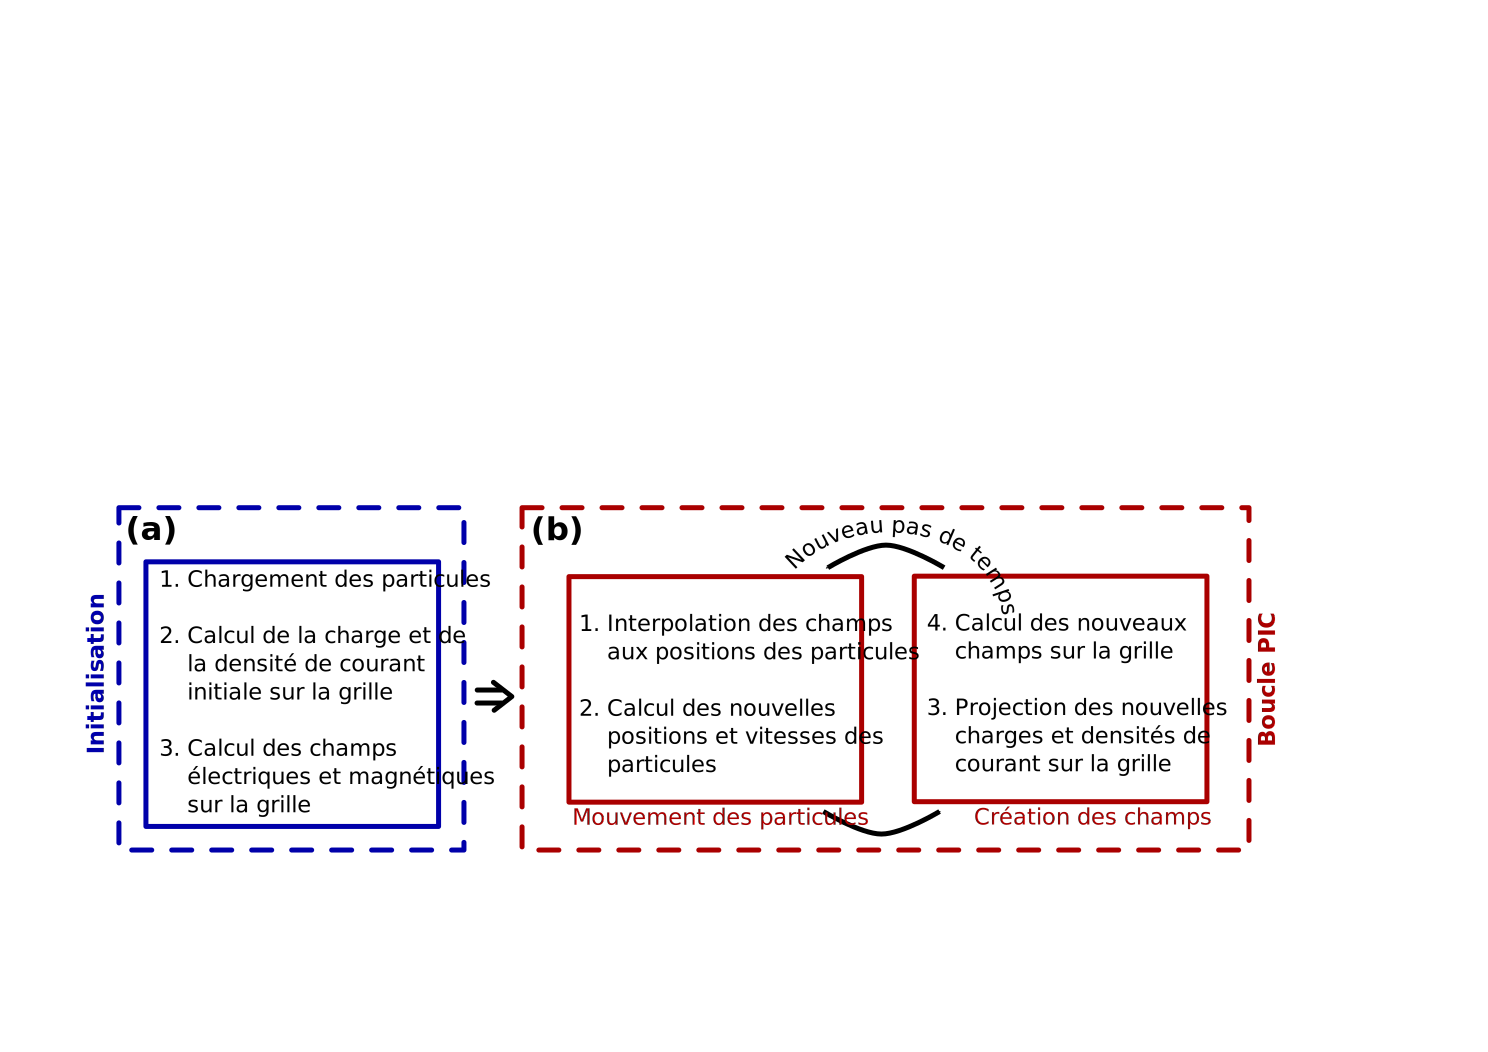
\includegraphics[width=\linewidth]{4-simulation/principe_PIC.png}
	\caption{Représentation schématique de l'algorithme d'un code PIC avec (a) les étapes principales de l'initialisation des macro-particules et des champs, et (b) les étapes principales de sa boucle temporelle.}
	\label{fig:4-PIC_algo}
\end{figure}

%\subsubsection{Conditions de bords}

Après que les nouvelles positions et vitesses des macro-particules aient été calculées, il est possible que ces dernières sortent de la boite de simulation. Elles peuvent alors être supprimées de la simulation, arrêtées dans la dernière maille, réfléchies selon une réflexion spéculaire, réinjectées depuis le bord opposé de la boite ou avec une impulsion tirée aléatoirement selon une loi Maxwellienne de température choisie à l'avance. 
De la même manière, les champs atteignant les bords de la boite peuvent être absorbés, réfléchis ou réinjectés au bord opposé de la boite.
Ces \textbf{conditions de bords} sont définies dans le fichier d'entrée de Smilei pour chaque bord et de manière indépendante pour les champs et chaque espèce de particule. 

Lors du calcul de l'évolution conjointe des champs et des particules, plusieurs \textbf{modules physiques additionnels} peuvent aussi être implémentés dans la simulation, tels que les collisions binaires entre particules, l'ionisation collisionelle ou l'ionisation par effet de champ (ionisation tunnel), ainsi que certains processus d'électrodynamique quantiques, tels que la production de photons par Compton Inverse multi-photon (ou \textit{synchrotron-like}) et la production de paires électron-positron par le processus Breit-Wheeler multi-photon. Pour le moment, les processus Bremsstrahlung et Bethe-Heitler ne sont cependant pas disponibles. Cette liste de module physique externes est néanmoins en constante évolution.
Les modèles de collisions binaires, d'ionisation collisionelle et d'ionisation par effet tunnel ont notamment été comparés à des résultats de modèles théoriques. Plus d'informations sont disponibles dans la documentation Smilei \parencite{derouillat_2018}.

Dans Smilei comme dans d'autres codes PIC, toutes les quantités physiques (charge, masse, énergie, champs électriques et magnétiques, …) sont normalisées à des quantités caractéristiques dépendantes de la pulsation du laser. Pour ne pas perdre en généralité, les quantités calculées à partir de ces codes sont donc souvent données en unités normalisées dans la littérature. Cependant, certains modules physiques externes de Smilei, comme par exemple l'ionisation par effet de champ, nécessitent que les unités physiques soient spécifiées dans la simulation. Dans ce cas, les simulations sont alors valides uniquement pour une pulsation laser bien définie. Puisque nous utiliserons ce type de module, dans le cadre de cette thèse nous spécifierons donc les quantités (distances, temps, …) en \textbf{unités physiques} usuelles (micromètres, picosecondes, …) et pas en unités du code.

\subsubsection{Diagnostics et outils d'analyse}

Afin de diminuer le volume de données à écrire sur le disque et faciliter leur analyse, Smilei est fourni avec des diagnostics pré-implémentés ainsi qu'un module d'analyse en \textit{Python} nommé happi. 
Ces derniers permettent d'étudier l'évolution des densités de charges, de courant et des champs dans la boite de simulation (via un \textit{DiagField}), ainsi que des quantités plus globales telles que l'énergie totale contenue dans la boite, ou l'énergie contenue dans les particules ou les champs (via un \textit{DiagScalar}). De plus, il est aussi possible de produire des histogrammes à partir des données de l'espace des phases, soit en considérant un instantané (temps fixé, via un \textit{DiagParticleBinning}), soit en intégrant temporellement une quantité à une position donnée (via un \textit{DiagScreen}).
Parmi les nombreux diagnostics disponibles, nous utiliserons principalement le diagnostic \textit{DiagField} permettant d'exporter les champs sur une grille prédéfinie, ainsi que le diagnostic \textit{DiagTrackParticles} permettant d'exporter l'espace des phases de particules satisfaisant une certaine condition. 

En géométrie 2D plane, la direction perpendiculaire au plan de simulation n'est pas simulée, et les poids statistiques des particules représentent un poids par unité de longueur et pas directement un nombre de particules. Le nombre de particules réelles peut être estimé en normalisant le poids statistique par une longueur caractéristique dans la dimension transverse, typiquement la taille de la tache focale du laser, ce qui reviens à supposer que la physique de l'interaction laser-plasma est relativement homogène sur cette longueur caractéristique.

Plus d'informations sur ces aspects sont disponibles dans la documentation officielle de Smilei \parencite{smilei_web}.

\subsection{Étude de paramètres numériques}

Dans la chaîne de simulations développée pour cette thèse, les simulations PIC sont les plus coûteuses en temps de calcul ; c'est pourquoi nous accordons ici un intérêt particulier à l'optimisation des paramètres numériques, en particulier la résolution spatiale et le nombre de particules par maille. De plus, cette étude nous permettra de nous assurer que les résultats obtenus ne varient pas significativement avec la résolution, le nombre de particules par maille, l'ordre d'interpolation ou l'ajout d'un module de collisions binaires.

\subsubsection{Définition des paramètres étudiés}

Nous considérons ici une situation typique où un laser d'\textbf{intensité $I_0=10^{20} \si{\W\per\cm^2}$} \textbf{polarisé linéairement}, de \textbf{longueur d'onde $1$ µm}, de \textbf{durée $30$ fs} (largeur à mi-hauteur) est focalisé avec une \textbf{tache focale de $5$ µm} (largeur à mi-hauteur) sur une \textbf{cible solide de polystyrène} $\rm (C_8 H_8)_n$ de densité électronique moyenne $300 ~ \rm n_c$, \textbf{d'épaisseur $15$ µm}, sur laquelle est collée un \textbf{absorbant homogène quasi-critique de polystyrène} de densité $0.96 ~ \rm n_c$ et d'épaisseur $11$ µm. Ces paramètres sont proches de ceux utilisés pour les simulations qui seront détaillées au chapitre \ref{chap:6-opti_numerique}. Ces paramètres et la géométrie de la simulation sont résumés en figure \ref{fig:4-PIC_boite_simu_validation}.

\begin{figure}[hbtp]
	\centering
	\includegraphics[width=0.5\linewidth]{4-simulation/boite_simu_validation.png}
	\caption{Dimensions caractéristiques de la boite de simulation PIC. Le laser se propage de gauche à droite, et les électrons sont exportés dans les 5 derniers µm du substrat.}
	\label{fig:4-PIC_boite_simu_validation}
\end{figure}

La simulation est effectuée dans une boite de \textbf{géométrie 2D plane} de $70$ µm $\times$ $70$ µm pendant $1$ ps. La cible est collée au bord arrière de la boite de simulation avec \textbf{conditions aux bords absorbantes} pour les particules et les champs électromagnétiques. 

La cible n'est \textbf{pas ionisée au début de la simulation}, et le \textbf{module d'ionisation par effet de champ} est \textbf{activé}. Les \textbf{atomes} sont aussi considérés parfaitement froids, et sont donc \textbf{immobiles avant l'arrivée du laser}. De cette manière, les particules proches des bords de la boite de simulation ne peuvent pas être absorbées par les conditions de bords avant d'avoir été influencées par le laser. Dans ce type de configuration, les électrons qui devraient physiquement être injectés dans le convertisseur collé au bord arrière du substrat (voir chapitre \ref{chap:3-methodes_exp}) sont donc supprimés de la simulation.

Les macro-électrons d'énergie cinétique supérieure à $m_e c^2$ sont exportés dès lors qu'ils se trouvent dans les $5$ derniers µm du substrat solide, en ne testant cette condition que tous les $5 ~ \si{\um/c} \approx 17 ~ \si{\fs}$ et en s'assurant de n'exporter chaque macro-particule qu'une seule fois par simulation (voir figure \ref{fig:4-PIC_boite_simu_validation}). Ce diagnostic permet de récupérer l'\textbf{espace des phases des électrons en face arrière du substrat} afin d'étudier les propriétés des sources d'électrons qui pourraient éventuellement être injectées dans des simulations \textit{Monte Carlo} du convertisseur, tel que cela sera effectué au chapitre \ref{chap:6-opti_numerique}. Les champs $\vec{E}$, $\vec{B}$ et les densités électroniques et ioniques sont aussi exportés dans une portion de la grille de $36$ µm $\times$ $30$ µm centrée sur l'axe de propagation laser et collée au bord droit, avec une résolution spatiale (mailles carrées) de $10$ mailles par longueur d'onde. L'export des champs et densités sur une grille plus petite que la grille de simulation permet de diminuer l'espace de stockage nécessaire à ce diagnostic.

L'\textbf{influence de la résolution spatiale} est étudiée, en considérant des mailles carrées ($\Delta y = \Delta x$) et une résolution temporelle fixée à $\Delta t = 0.95 \Delta x/\sqrt{2}$ de façon à satisfaire la condition Courant-Friedrichs-Lewy en géométrie 2D plane (voir équation (\ref{eq:4-PIC_CFL})). L'\textbf{influence du nombre d'ions par mailles} est elle aussi étudiée (il n'y a pas de macro-électrons au début de la simulation ; ceux-ci étant créés par ionisation).
Nous considérons un cas de référence avec une résolution spatiale de $60$ mailles par longueur d'onde, et avec $10$ macro-ions d'hydrogène ($\rm H$) et 10 macro-ions de carbone ($\rm C$) par maille. Un cas à haute résolution est aussi étudié, avec une résolution spatiale de $80$ mailles par longueur d'onde et 10 macro-ions (10 de $\rm H$ + 10 de $\rm C$) par mailles. L'\textbf{influence de l'ordre d'interpolation}, ainsi que l'effet des \textbf{collisions électrons-ions} (avec ionisation collisionnelle) est aussi étudiée pour le cas à haute résolution. Ce dernier cas est donc le plus précis, et nous permettra de déterminer s'il est possible de retrouver des résultats similaires avec des simulations plus rapides (résolution et nombre de macro-ions par maille plus faible, collisions désactivées). 

Les simulations ont été lancées sur 20 noeuds manycores (64 coeurs par noeud, soit 1280 coeurs au total) de la partition Irene-KNL du super-calculateur TGCC Joliot-Curie (CEA Bruyères-le-Châtel) avec 4 processus \textit{MPI} par noeud (soit 16 coeurs par processus \textit{MPI}) et 32 threads \textit{OpenMP} par processus \textit{MPI} (hyper-threading conseillé par J. Derouillat de l'équipe de Smilei sur cette machine). La boite de simulation est découpée en $128 \times 128$ patches (environ 6 patches par thread) avec un load balancing toutes les 20 itérations. Afin de satisfaire le découpage en patches pour toutes les simulations, la taille de la boite de simulation est automatiquement ajustée en ajoutant du vide devant la cible. La version de Smilei utilisée est la version 4.5, et la vectorisation n'a pas été activée. Plus de détails sur les techniques de parallélisation sont disponibles dans la documentation de Smilei \parencite{smilei_web}, et le vocabulaire utilisé est défini (en anglais) en référence \parencite{vocab_parallelisation}. 

\subsubsection{Temps de calcul et convergence des résultats}

Le tableau \ref{tab:4-temps_calcul_PIC} résume les paramètres numériques utilisés pour cette étude, et indique le temps de calcul correspondant, en heure CPU (hCPU), pour toutes ces simulations. Les diagnostics de champs occupent un espace de stockage d'environ $800$ Mo pour chaque simulation, tandis que le diagnostic d'espace des phases des particules nécessite entre $200$ Mo (pour le cas \textit{IV}) et $5$ Go de stockage (pour le cas \textit{VII}). L'espace stockage nécessaire pour les autres fichiers de diagnostics est négligeable.
Le \textbf{temps de calcul} est \textbf{très dépendant de la résolution et du nombre de macro-particules par mailles} ; un plus grand nombre de macro-ions par maille et une résolution plus importante (donc un nombre de mailles plus important) nécessitant plus d'opérations de calcul. L'utilisation d'un ordre d'interpolation de $2$ diminue le temps de calcul de $40 \%$ pour le cas à haute résolution, alors que l'activation du module de collisions l'augmente d'un facteur $>2$. Pour le cas de référence, diviser le nombre de particules par $2$ permet de diminuer le temps de calcul de $40 \%$ tandis que diviser le nombre de particules par $10$ diminue le temps de calcul d'un facteur $> 4$.

\begin{table}
\centering
\begin{tabular}{ | l | l | l | l | l || l | }
    \hline
            & Résolution    & Nombre        & Ordre             & Collisions    & Temps total \\
    Label   & spatiale      & d'ions/maille & d'interpolation   & activées      & en hCPU \\
    \hline
    \textit{I}   & 40 mailles/$\lambda_L$ & 10          & 4         & Non        & 1583     \\
    \textit{II}  & 60 mailles/$\lambda_L$ & 10          & 4         & Non        & 3866     \\
    \textit{III} & 60 mailles/$\lambda_L$ & 5           & 4         & Non        & 2224     \\
    \textit{IV}  & 60 mailles/$\lambda_L$ & 1           & 4         & Non        & 899      \\
    \textit{V}   & 80 mailles/$\lambda_L$ & 10          & 4         & Non        & 8054     \\
    \textit{VI}  & 80 mailles/$\lambda_L$ & 10          & 2         & Non        & 5847     \\
    \textit{VII} & 80 mailles/$\lambda_L$ & 10          & 4         & Oui        & 18496    \\
    \hline
    \end{tabular}
    \caption{Définition des paramètres numériques étudiés, et temps de calcul correspondant. Le cas de référence est le cas \textit{II}, et le cas à haute résolution est le cas \textit{V}. Les autres cas présentent des variations par rapport à ces derniers.}
	\label{tab:4-temps_calcul_PIC}
\end{table}


L'analyse de l'énergie totale contenue dans la boite nous permet d'étudier le chauffage numérique éventuel des électrons. L'évolution de l'énergie totale dans la boite de simulation, ainsi que l'énergie cinétique contenue dans toutes les espèces (électrons et ions) est tracée en fonction du temps en figure \ref{fig:4-PIC_chauffage_numerique}. Pour chacune de ces simulations, l'énergie totale augmente au début de la simulation à cause de l'injection du laser dans la boite. Nous pouvons ensuite observer que la physique du \textbf{transfert d'énergie} entre le laser et le plasma (autour de $(50 ~ \si{[\um/c]} + \tau_{FWHM}) \sim 0.2$ ps) semble assez \textbf{similaire} pour ces différents cas. Aux \textbf{temps plus longs}, on observe cependant pour certaines simulations que l'\textbf{énergie cinétique des espèces augmente avec le temps}, faisant aussi augmenter l'énergie totale contenue dans la boite. Ce type de comportement non physique est caractéristique du phénomène de \textbf{chauffage numérique}.
Nous pouvons aussi observer que pour le cas à haute résolution sans collisions \textit{V}, les \textbf{énergies cinétiques et totales} tendent plutôt à légèrement \textbf{diminuer avec le temps}. Ceci peut être expliqué qualitativement comme la conséquence des \textbf{conditions aux bords absorbantes} pour les particules et les champs, qui peuvent sortir de la boite et emporter une partie de l'énergie avec eux. Le cas de référence \textit{II} ainsi que son équivalent avec 5 macro-ions par maille \textit{III} et le cas à plus basse résolution \textit{I} sont superposés au cas \textit{V}.
Lorsque le nombre de macro-ions par mailles est faible, comme pour le cas de référence avec $1$ macro-ion par maille \textit{IV}, l'énergie totale dans la boite semble surestimée aux temps longs et on observe un léger chauffage numérique. L'ordre d'interpolation semble aussi jouer un rôle important car, même avec la plus haute résolution et $10$ macro-ions par mailles, la simulation \textit{VI} comprenant un ordre d'interpolation de $2$ subit du chauffage numérique aux temps longs. Le module de collisions semble aussi jouer un rôle non négligeable dans le chauffage numérique des électrons aux temps longs, comme nous pouvons le remarquer sur la courbe du cas \textit{VII}. 

\begin{figure}[hbtp]
	\centering
	\includegraphics[width=0.7\linewidth]{4-simulation/comparaison_U.png}
	\caption{Comparaison des énergies totales (traits pleins) et cinétiques (traits pointillés) contenues dans toute la boite de simulation, pour les différentes simulations étudiées. Les cas \textit{I},\textit{II}, \textit{III} et \textit{V} sont superposés.}
	\label{fig:4-PIC_chauffage_numerique}
\end{figure}

Nous pouvons ensuite traiter l'espace des phases des \textbf{électrons exportés en face arrière du substrat avec une énergie cinétique supérieure à $m_e c^2$} afin de comparer leurs distributions en énergie, leurs distributions en angle polaire, leurs distributions spatiales transverse ainsi que leurs temps d'export dans le diagnostic (affichés respectivement en figures \ref{fig:4-PIC_validation_electrons}a, \ref{fig:4-PIC_validation_electrons}b, \ref{fig:4-PIC_validation_electrons}c et \ref{fig:4-PIC_validation_electrons}d).
Le cas \textit{IV} comprenant le moins de particules par maille est le plus dispersé en queue de distribution en énergie et en angle. Il est aussi spatialement moins piqué, et la charge totale du faisceau d'électrons (donc leur nombre total, non représenté ici) est inférieure aux autres cas (65 nanocoulombs contre 70 à 75 nanocoulombs pour les autres simulations). 
Tous les autres cas sont quantitativement assez proches pour ces diagnostics. En particulier, nous pouvons donc en conclure que l'effet des collisions est relativement limité dans ce type de simulations. Compte tenu de la similarité de ces résultats lorsque nous considérons uniquement les électrons \textbf{exportés dans le diagnostic} et dont \textbf{l'énergie cinétique est supérieure à $m_e c^2$}, nous pouvons en déduire que les effets de \textbf{chauffage numérique} précédemment décrits concernent principalement les \textbf{électrons qui sont peu énergétiques et ne sont pas éjectés en face arrière de la cible}. 
Nous pouvons observer que, pour ces électrons, la distribution spatiale transverse du faisceau est relativement piquée autour de l'axe de propagation, ce qui semble montrer que la taille transverse de la boite de simulation est suffisamment importante. Une distribution spatiale plus plate aurait en effet au contraire indiqué qu'un nombre non négligeable d'électrons aurait pu quitter la boite sur les bords avant d'être exporté en face arrière du substrat. 
Le nombre d'électrons d'énergie cinétique supérieure à $m_e c^2$ exportés est relativement négligeable après $0.8$ ps, ce qui semble indiquer que l'interaction du laser avec la cible a été décrite suffisamment longtemps pour ces particules et que le temps de simulation choisi est suffisamment important. 

\begin{figure}[hbtp]
	\centering
	\includegraphics[width=\linewidth]{4-simulation/Smilei_validation.png}
	\caption{Comparaison de différentes caractéristiques des sources d'électrons pour les différentes simulations étudiées, avec (a) leurs distributions en énergie, (b) leurs distributions angulaire, (c) leurs distributions spatiale transverse et (d) leurs distributions temporelle.}
	\label{fig:4-PIC_validation_electrons}
\end{figure}

Compte tenu des résultats très similaires obtenus pour les sources d'électrons avec ces différents paramètres de simulations, le cas à faible résolution avec 10 macro-ions (10 $\rm C$ + 10 $\rm H$) par maille \textit{I}, ou le cas de référence avec 5 macro-ions par mailles \textit{III} seraient a priori suffisants pour cette situation, et il ne serait pas très intéressant d'utiliser une résolution importante comme le cas \textit{V}. L'utilisation d'un ordre d'interpolation de $2$ avec le cas \textit{VI} ou d'un seul macro-ion par maille avec le cas \textit{IV} permet de faire diminuer le temps de calcul mais augmente le chauffage numérique. L'utilisation du module de collisions dans le cas \textit{VI} augmente considérablement le temps de calcul et n'amène pas de modifications significatives de nos résultats.
Afin de bénéficier d'une bonne statistique, les paramètres de notre cas de référence avec 10 macro-ions par maille \textit{III} seront utilisés comme base pour l'étude que nous mènerons au chapitre \ref{chap:6-opti_numerique}, où ce type de simulation sera aussi analysé plus en détails.

\section{Modélisation de la propagation de particules dans la matière}

Une fois que des électrons ont été accélérés par le laser, nous cherchons à les injecter dans un convertisseur afin de transférer une partie significative de leur énergie cinétique en photons $\gamma$.

\newpage

Comme nous l'avons vu au chapitre \ref{chap:1-particules}, la longueur caractéristique de perte d'énergie par rayonnement est nommée longueur de radiation, et est de l'ordre de quelques millimètres pour des matériaux de densité et numéro atomique élevés (e.g. $\sim 3 ~ \si{\mm}$ pour du platine). Pour ce type de matériaux et d'épaisseurs, nous nous attendons aussi à ce que les effets collisionnels jouent un rôle majeur pour la propagation des électrons dans le convertisseur (voir chapitre \ref{chap:1-particules}).
Ainsi, bien que les codes PIC puissent en théorie être utilisés pour simuler la propagation d'électrons dans le convertisseur, ce type d'épaisseurs est prohibitif en terme de temps de calcul, en particulier pour des simulations à 2 ou 3 dimensions de matériaux denses (nécessitant donc une résolution importante), et avec des modules physiques de collisions activés.

Au contraire, la propagation de particules dans la matière dans des régimes collisionnels est très souvent étudiée à l'aide d'algorithmes de transport de type \textit{Monte Carlo} (noté MC), où les épaisseurs de solide simulées peuvent facilement atteindre plusieurs centimètres voire mètres \parencite{agostinelli_2003}. Pour ce type d'applications, cette approche est \textbf{beaucoup moins coûteuse en temps de calcul} que les codes PIC ou hybrides, et peut donc permettre d'étudier une grande variété de matériaux et d'épaisseurs de convertisseurs en un temps raisonnable. Ces codes reposent cependant sur l'hypothèse que \textbf{le matériau n'est pas modifié par le passage des particules} (la densité et les sections efficaces sont constantes), et que les \textbf{particules injectées} peuvent être considérées \textbf{indépendantes les unes des autres}. Ainsi, pour utiliser ce type de méthode il doit être possible de considérer que les \textbf{effets collisionnels} sont \textbf{dominants sur les effets collectifs} lors de la propagation du faisceau (à l'opposé des codes PIC dont l'intérêt réside justement dans la modélisation de ces effets collectifs et où les collisions sont par défaut négligées).

Dans l'étude numérique que nous mènerons au chapitre \ref{chap:6-opti_numerique}, les électrons accélérés dans le code PIC Smilei seront injectés dans une application Monte Carlo nommée gp3m2 (présentée dans cette section) qui nous permettra de simuler leur propagation dans le convertisseur. Pour transférer les électrons simulés via le code PIC dans le code MC, nous choisirons de \textbf{simuler le substrat dans ces deux codes}, et d'\textbf{injecter les particules dans le code MC à leur position d'export dans le code PIC} (voir figure \ref{fig:4-MC_PIC_transition}), avec leur \textbf{impulsion et temps correspondant}. 

\newpage 

Dans ce type de situations, les hypothèses inhérentes à la méthode Monte Carlo nous contraignent néanmoins à supposer que le faisceau d'électrons a un comportement différent dans les deux types de simulations, malgré des caractéristiques identiques (même espace des phases). Pour la propagation des électrons dans un convertisseur froid, dense et de numéro atomique élevé, on peut néanmoins justifier cette hypothèse qualitativement en notant que, dans ce type de matériau, la propagation du faisceau est très fortement influencée par les diffusions, car celles-ci y sont très fréquentes (voir chapitre \ref{chap:1-particules}). Ces effets collisionnels tendent par conséquent à limiter l'importance relative des effets collectifs.
L'effet des \textbf{champs électromagnétiques} en face avant de la cible ainsi que le \textbf{courant de retour d'électrons froids} sont eux aussi \textbf{négligés dans le convertisseur}, bien qu'ils puissent jouer un rôle significatif dans la propagation des électrons énergétiques dans la matière \parencite{davies_1997, compantlafontaine_2018}. Pour un convertisseur suffisamment épais, on s'attend à ce que le phénomène d'écrantage atténue l'effet des champs électromagnétiques situés hors du convertisseur, et limite donc leur influence sur la propagation du faisceau de particules. La justification rigoureuse de ces hypothèses nécessiterait néanmoins une étude approfondie. Différents aspects de ce problème sont discutés notamment dans les références \parencite{davies_2002, tikhonchuk_2002, davies_1997, compantlafontaine_2018}. 

\begin{figure}[hbtp]
	\centering
	\includegraphics[width=0.7\linewidth]{4-simulation/transition_PIC_MC.png}
	\caption{Schéma de principe du transfert de données entre les codes Particle-In-Cell et Monte Carlo. Les particules enregistrées dans le substrat dans le code PIC sont réinjectées à leur position d'export dans le code Monte Carlo.}
	\label{fig:4-MC_PIC_transition}
\end{figure}

Dans cette section, nous étudierons tout d'abord le principe de base d'un algorithme de transport \textit{Monte Carlo}, ainsi que les spécificités des outils Geant4. Nous présenterons ensuite l'application gp3m2 développée dans le cadre de cette thèse. Celle-ci sera utilisée au chapitre \ref{chap:6-opti_numerique} pour simuler la production d'une sources de photons $\gamma$ via le processus Bremsstrahlung, et en utilisant la méthode décrite précédemment pour le transfert de données depuis le code PIC. Cette application est néanmoins adaptée à un grand nombre d'autres situations, tel que cela sera notamment évoqué au chapitre \ref{chap:6-opti_numerique}. 

\subsection{Principe des outils \textit{Monte Carlo} Geant4}

Geant4 (pour GEometry ANd Tracking) est un ensemble d'outils logiciels pour l'étude numérique de la propagation de particules dans la matière. Ses domaines d'applications incluent la physique des hautes énergies et des accélérateurs, la physique nucléaire, médicale ou encore l'astrophysique.



Ces outils open-source sont développés en \textit{C++} orienté objet par une large collaboration internationale, et implémentent de nombreuses fonctionnalités pour la production d'une application \textit{Monte Carlo}. La philosophie très modulaire de Geant4 lui permet d'être applicable à un grand nombre de situations différentes, notamment en termes de processus et de modèles physiques (traitement des énergies de quelques eV à plusieurs TeV), selon des géométries complexes, et avec des sources de particules primaires et des diagnostics personnalisables. Bien que de nombreux exemples d'applications soient fournis avec le code source, aucun n'était néanmoins adapté au traitement complet de l'espace des phases aussi bien en entrée qu'en sortie de code. Une application nommée gp3m2 (pour Geant4 simulation of Particle Phase-space Propagation in a Multi-layer Material) a donc été développée durant cette thèse pour répondre à ce besoin.


Plus d'informations sur les outils Geant4 sont disponibles dans les références \parencite{agostinelli_2003, allison_2006, allison_2016}. Une documentation pratique est aussi disponible sur son site officiel \parencite{geant4_web}, où il est notamment possible de consulter les \textit{Physics Reference Manual} et \textit{Application Developper Guide}. Ces documents, dont la prochaine section est en partie inspirée, permettent de se renseigner respectivement sur la physique simulée et sur la façon d'implémenter les classes Geant4 dans sa propre application. Une documentation pour l'application gp3m2 est disponible sur son dépot github \parencite{gp3m2}. Plus d'informations sur la méthode \textit{Monte Carlo} peuvent notamment être trouvées dans la référence \cite{haghighat_2015}.

\subsubsection{Algorithme \textit{Monte Carlo} pour le transport de particules}

Dans un code \textit{Monte Carlo} de transport de particules (abrégé en code \textit{Monte Carlo}, ou code MC), les particules injectées dans la simulation sont appelées \textit{particules primaires}, tandis que celles produites lors de processus physiques sont appelées \textit{particules secondaires}. Afin de limiter le nombre de particules simulées, ces codes se basent eux aussi sur un échantillonnage de la fonction de distribution via des \textbf{macro-particules} auxquelles sont assignés un \textbf{poids statistique arbitraire}. Ces dernières n'ont cependant pas de facteur de forme spatial comme pour les codes PIC. Le nombre de macro-particules $N$ doit être suffisamment important pour correctement échantillonner la fonction de distribution, et le rapport signal sur bruit varie en $\sqrt{N}$ \parencite{haghighat_2015}.

Lorsque ces particules (primaires ou secondaires) se propagent dans la matière, elles peuvent interagir avec le milieu environnant par l'intermédiaire de différents processus, dont les plus significatifs ont été évoqués au chapitre \ref{chap:1-particules} (ionisation, diffusions élastiques, etc ...). La probabilité d'interaction de chaque processus est usuellement modélisée par une section efficace notée $\sigma$, et ces \textbf{interactions} sont supposées \textbf{ponctuelles} et \textbf{indépendantes} les unes des autres.

Dans ce cas, il est possible de montrer (voir chapitre 2 de la référence \parencite{rax_2007}) que la probabilité de \textbf{ne pas interagir pendant une distance $\ell$} est donnée par \parencite{geant4_physref, haghighat_2015} :
\begin{equation}
    P(\ell)= \exp\left(-\dfrac{\ell}{\ell_{int}}\right)~ \rm ,
\end{equation}
où $\ell_{int}$ est une longueur d'interaction typique \textbf{pour ce processus dans ce matériau} aussi appelée \textit{libre parcours moyen}, et qui s'exprime comme :
\begin{equation}
    \ell_{int} = \dfrac{1}{n ~ \sigma} ~ \rm ,
\end{equation}
avec $\sigma$ la section efficace du processus considéré, et $n$ la densité de particules cibles dans le matériau.
Dans les codes Monte Carlo, un tirage aléatoire permet alors de générer une distance de parcours \textbf{pour ce processus dans ce matériau} via \parencite{haghighat_2015} :
\begin{equation}
    \ell = - \ell_{int} \times \ln{\eta} ~ \rm ,
\end{equation}
où $\eta$ est une variable aléatoire uniforme dans $[0,1[$.

Lors de la création d'une particule simulée, une longueur de parcours $\ell$ est tirée aléatoirement \textbf{pour chaque processus}, chacun ayant un libre parcours moyen et un état final potentiellement différents (dépot d'énergie, création de particules secondaires, ...). Le processus effectivement mis en oeuvre est alors celui ayant \textbf{la distance la plus courte}, et les autres longueur de parcours sont ensuite modifiées pour prendre en compte la distance déjà parcourue, notée ici $\Delta \ell$ \parencite{haghighat_2015}. L'intervalle entre deux interactions physiques est appelé \textit{Step} dans le langage de Geant4. Cet algorithme est représenté schématiquement en figure \ref{fig:4-MC_algo}. 

\begin{figure}[hbtp]
	\centering
	\includegraphics[width=\linewidth]{4-simulation/principe_MC.png}
	\caption{Principe d'un code \textit{Monte Carlo}, où (a) les libres parcours moyens sont calculés lors de initialisation, puis (b) une distance au prochain point d'interaction est tirée aléatoirement en fonction du libre parcours moyen. Le processus ayant la distance la plus courte est choisi et mis en œuvre, puis (c) une nouvelle distance est tirée pour ce processus pendant que les distances au point d'interaction sont mises à jour pour les autres processus. Le processus ayant la distance la plus courte est alors mis en œuvre, et l'étape (c) recommence.}
	\label{fig:4-MC_algo}
\end{figure}

Dans Geant4, le tirage aléatoire est en fait effectué non pas sur la distance de parcours $\ell$ du \textit{Step} courant, mais plutôt sur le \textbf{nombre de libre parcours moyens} correspondant $N_{\ell_{int}}$ (cette astuce permet notamment de faciliter le calcul de la distance de parcours lors d'un changement de matériau) \parencite{geant4_physref, agostinelli_2003} :
\begin{equation}
    N_{\ell_{int}}=\dfrac{\ell}{\ell_{int}} = - \ln\eta ~ \rm ,
\end{equation}
et après chaque étape de calcul, pour chaque processus le nombre de libre parcours moyen restants $N_{\ell_{int}}'$ est alors mis à jour \parencite{geant4_physref} :
\begin{equation}
    N_{\ell_{int}}'=N_{\ell_{int}} - \dfrac{\Delta \ell}{\ell_{int}} ~ \rm ,
\end{equation}
ainsi que le temps associé à la particule (dans le référentiel du laboratoire) \parencite{geant4_physref} :
\begin{equation}
    t_f = t_i +  \dfrac{\Delta \ell}{2}\left(\dfrac{1}{v_i}+\dfrac{1}{v_f}\right) ~ \rm ,
\end{equation}
avec $v_i$ et $v_f$ les vitesses de la particule respectivement au point d'interaction précédent et au point d'interaction courant, et $t_i$ et $t_f$ les temps correspondant respectivement à l'interaction précédente et courante.

Le parcours des particules est aussi arrêté par les interfaces entre différent matériaux, et plus généralement lors de tout changement de volume défini dans la simulation (appelé \textit{volume logique}) sans forcement qu'il y ait changement de matériau. Ce comportement sera d'ailleurs mis à profit dans notre application décrite dans la prochaine section.

Ces étapes de calcul sont répétées de la création à la destruction de la particule simulée. 

\subsubsection{Processus et modèles physiques}

Dans certains cas, simuler toutes les interactions discontinues (ou discrètes) des particules lors de leur propagation n'est néanmoins pas très efficace, et certaines techniques permettent d'améliorer le temps de calcul. 
En effet, lorsque des particules se propagent dans la matière, elles peuvent produire un très grand nombre de particules secondaires, par ionisation par exemple. Nombre de ces particules secondaires sont cependant très peu énergétiques, et se propagent donc sur une distance très faible (voir chapitre \ref{chap:1-particules}). Dans Geant4, une distance appelée \textit{range cut} est donc définie par l'utilisateur, et les particules secondaires n'ayant que très peu de chances de se propager sur cette distance caractéristique ne sont pas générées \parencite{geant4_physref}. Cette technique permet ainsi de diminuer grandement le nombre de particules secondaires à simuler, et l'énergie emportée par ces particules est simplement considérée comme une \textbf{perte d'énergie continue} pour la particule incidente \parencite{geant4_physref}. 
De plus, pour les processus très fréquents impliquant une variation d'énergie faible et une déviation angulaire faible, tels que la perte d'énergie par ionisation ou les diffusions multiples pour les électrons (voir chapitre \ref{chap:1-particules}), il est numériquement très coûteux de simuler individuellement chaque interaction de la particule incidente avec la matière, et ces processus sont aussi considérés comme \textbf{continus} \parencite{geant4_physref}. L'effet des diffusions multiples est quant à lui calculé et ajouté à la trajectoire de la particule à la fin de chaque \textit{Step} \parencite{geant4_physref}. 
La plupart des autres processus (Bremsstrahlung, création de paires, ...) sont néanmoins décrits de façon discrète, tel que cela a été présenté précédemment.
D'autres techniques plus avancées (roulette russe, biaising, ...) permettent aussi d'améliorer la convergence du calcul mais ne seront pas discutées dans le cadre de cette thèse.

Ces différents processus, discrets ou continus, sont implémentés par différents modèles théoriques, semi-empiriques, ou jeux de données expérimentales. Bien qu'il soit possible à l'utilisateur de choisir quels modèles utiliser dans quelles conditions (et même d'ajouter ses propres processus et modèles), Geant4 propose toutefois des \textbf{listes de processus physiques et de modèles déjà définis} et adaptés à différentes situations physiques et gammes d'énergies, comme par exemple la physique des photons optiques, des interactions électromagnétiques, ou de la décroissance des particules instables. Certaines de ces listes (appelées \textit{reference PhysicsLists} dans Geant4) ont de plus été activement validées contre des données expérimentales \parencite{geant4_val}.

Les propriétés de la plupart des matériaux et de la plupart des particules sont aussi déjà implémentées dans ces outils de base, mais il est toujours possible d'ajouter de nouveaux matériaux ou particules si besoin.

\subsubsection{Autres fonctionnalités}

En plus de la gestion des processus physiques et du transport des particules, Geant4 propose de nombreux outils permettant de s'adapter à des contextes très variés. Nous mentionnerons simplement les outils pour la création d'une \textbf{géométrie}, où les volumes de matières peuvent être définis à partir de volumes simples (pavés, cylindres, …) et d'opérations entre ceux ci (répétitions, union, différence, …), ainsi que des outils pour la \textbf{définition des propriétés des particules primaires}, la production semi-automatisée d'histogrammes pour l'\textbf{analyse des données générées par la simulation}, ou encore des outils de \textbf{visualisation} de la trajectoire des particules, ... Plus d'informations sont disponibles dans la référence \parencite{geant4_appdev}.


\subsection{Présentation de l'application gp3m2}

Pour produire une source de photons $\gamma$ adaptée à l'étude du processus BWL, nous aurons besoin d'optimiser l'épaisseur de convertisseurs pour chaque source d'électrons produite dans nos simulations PIC. Nous chercherons donc à définir les propriétés des particules primaires injectées dans notre application Monte Carlo à partir de l'espace des phases des électrons générés par le code PIC (voir figure \ref{fig:4-MC_PIC_transition}). Pour pouvoir réutiliser les données générées dans d'autres codes (notamment le code TrILEns présenté dans la section suivante), il nous sera aussi nécessaire d'exporter l'\textbf{espace des phases des particules} qui \textbf{sortent du convertisseur}.

Pour répondre à ces objectifs, une application nommée gp3m2 a été développée dans le cadre de cette thèse à partir des outils Geant4, et est disponible en open source avec une documentation sur le dépot github \parencite{gp3m2}.

\subsubsection{Physique simulée}

Dans cette application, le convertisseur est considéré \textbf{cylindrique}, et est placé au centre d'une boite vide (matériau \textit{G4\_Galactic}) de dimensions 1 m $\times$ 1 m $\times$ 1 m.

Dans toutes nos simulations nous utiliserons la liste de processus physique (\textit{reference physics list}) nommée \textit{G4EmStandard\_option4}, car elle est considérée comme étant la plus précise pour les interactions électromagnétiques dans une large gamme d'énergie (de 1 keV à 100 TeV) \parencite{geant4_physref}. Parmi les processus implémentés les plus importants, nous pouvons notamment mentionner les diffusions multiples, l'ionisation, la production de photons par Bremsstrahlung et l'annihilation pour les électrons et les positrons, ainsi que la photo-ionisation, les diffusions Rayleigh, Compton et la production de paires électron-positron pour les photons (voir chapitre \ref{chap:1-particules}).

Sauf indications contraires le \textit{range cut} est fixé à 10 µm, et les propriétés des matériaux utilisés sont définies à partir des données du NIST, implémentées par défaut dans Geant4.

\subsubsection{Injection des particules primaires}

Afin de pouvoir étudier une large gamme de sources d'électrons différentes, les \textbf{propriétés des particules primaires} sont définies \textbf{à partir d'un fichier d'espace des phases}, qui est lu au début de la simulation. Ce type de fichier peut être \textbf{produit à partir de données de simulations PIC} par exemple, mais peut aussi être \textbf{généré à partir de distributions en énergie, en angle, en espace et en temps} déterminées, notamment via certains outils du module p2sat (module présenté à la fin de ce chapitre).

Dans ce fichier, la première colonne correspond au le poids statistique $w$ des macro-particules, tandis que la seconde, troisième et quatrième colonne contiennent respectivement les positions $x$, $y$, $z$ des particules. Les trois colonnes suivantes contiennent quant à elles la projection des impulsions des macro-particules selon $x$, $y$, $z$ notées $p_x$, $p_y$, $p_z$, et la dernière correspond au temps $t$ auquel ces informations ont été exportés. \textbf{Chaque ligne} de ce fichier décrit donc \textbf{une macro-particule}, et son \textbf{numéro de ligne} est un nombre entier qui peut permettre de \textbf{l'identifier}.

Lors de la création des particules primaires, nous définissons leurs poids statistiques, positions, impulsions et temps selon un \textbf{tirage aléatoire dans la liste de macro-particules du fichier d'entrée}. Nous générons donc aléatoirement un identifiant de particule ($\approx$ numéro de ligne), et définissons les propriétés des particules primaires à partir de la macro-particule correspondante. Ce type de tirage est \textbf{indépendant du poids statistique} de la macro-particule considérée, et \textbf{permet de bien représenter les configurations avec un poids statistique faible}. Les poids statistiques ayant été préalablement normalisés pour indiquer un nombre de particules réelles, il nous est aussi nécessaire de diviser chacun des poids $w$ par le nombre total de macro-particules tirées lors de la simulation, afin de conserver le nombre total de particules réelles représentées dans la simulation, et ce indépendamment du nombre de particules primaires simulées.

Pour un calcul parallélisé sur $N$ coeurs ce fichier est lu et sauvegardé en mémoire $N$ fois, et il sera donc nécessaire de veiller à ne pas fournir un fichier d'entrée trop lourd pour les capacités de la machine utilisée. Un algorithme de réduction de données d'espace des phases a été développé notamment pour cet effet, et celui-ci sera présenté à la fin de ce chapitre. De futurs développements pourraient permettre de limiter l'espace mémoire nécessaire en ne lisant qu'une seule fois le fichier d'entrée, et en partageant les informations entre les différents coeurs.

\subsubsection{Diagnostics}

Les particules primaires ainsi définies vont donc pouvoir interagir avec le convertisseur via les processus considérés dans la liste de processus physique. Pour une source d'électrons injectée donnée, nous pourrons chercher à optimiser les caractéristiques des sources de photons $\gamma$ produites en faisant varier l'épaisseur du convertisseur. Il nous serait aussi intéressant de pouvoir estimer les propriétés des sources d'électrons et positrons produits, qui pourraient contribuer au bruit de mesure expérimental. 

Pour récupérer ces informations, \textbf{l'espace des phases} (poids statistique, impulsion, position et temps) \textbf{de chaque particule} (photon $\gamma$, $e^-$, $e^+$) \textbf{s'échappant de la cible est sauvegardé}. Plus précisément, nous enregistrons l'espace des phases de chaque particule dès lors que celle-ci est arrêtée par un changement de volume logique, en effectuant un test à chaque \textit{Step}. De cette façon, l'espace des phases des particules d'un type donné est exporté \textbf{dans le même fichier}, et ce \textbf{indépendamment de sa position d'export} (par la face arrière du convertisseur, sa face avant ou ses bords). La détermination des propriétés de la source de particules éjectés spécifiquement en face arrière devra être effectuée en \textbf{post-traitement}, en filtrant les particules par leur position d'export. Ce type de géométrie est illustré par exemple en figure \ref{fig:4-MC_tranches_gp3m2}a, où les bords et la face avant du convertisseur ne sont pas représentés par souci de simplicité.

Pour une source d'électrons et un matériau donné, nous pouvons alors imaginer \textbf{optimiser l'épaisseur du convertisseur} en comparant les résultats obtenus par un \textbf{nombre $N$ de simulations différentes}, \textbf{en faisant} par exemple \textbf{varier l'épaisseur du convertisseur} de $0$ à $L$ ($L$ étant l'épaisseur maximale considérée) avec un pas constant de $\Delta L = L/N$. 
Bien que cette approche puisse être en principe suffisante, une \textbf{précision importante sur l'épaisseur} optimale du convertisseur ($\Delta L$ faible) nécessiterait un \textbf{nombre de simulations important}, et ce type de simulations serait relativement \textbf{peu efficace en terme de temps de calcul}.

Pour expliquer ceci, considérons tout d'abord une optimisation simplifiée avec seulement deux épaisseurs de convertisseurs $\Delta L$ et $2 \Delta L$. Dans la première simulation d'épaisseur $\Delta L$, représentée en figure \ref{fig:4-MC_tranches_gp3m2}a, des électrons sont injectés dans le convertisseur, se propagent et interagissent avec le matériau (dépôt d'énergie, diffusions, production de particules secondaires, ...). Les particules (primaires comme secondaires) ayant atteint la face arrière du convertisseur après avoir traversé une épaisseur $\Delta L$ de matière sont exportées puis sortent de la boite de simulation et sont détruites (on néglige l'export par la face avant ou par les bords pour cette explication par souci de clarté, même si cela ne change rien au fond du propos). De la même manière, dans la simulation d'épaisseur $2 \Delta L$ illustrée en figure \ref{fig:4-MC_tranches_gp3m2}b, les particules injectées se propagent, peuvent éventuellement produire des particules secondaires, et ces particules seront exportées puis détruites après avoir traversé une épaisseur $2 \Delta L$ de matière. Néanmoins, puisque les interactions dans la matière sont considérées \textbf{indépendantes} les unes des autres, nous pouvons considérer que, aux fluctuations statistiques près, les \textbf{propriétés des faisceaux de particules} se propageant dans les deux convertisseurs sont \textbf{similaires dans les deux simulations à une profondeur $<\Delta L$ donnée}. Pour ces profondeurs, la propagation de ces particules est donc simulée $2$ fois (1 fois par simulation) et \textbf{coûte donc du temps de calcul sans améliorer la précision des résultats}. L'ajout d'une troisième simulation d'un convertisseur d'épaisseur $3 \Delta L$, illustré en figure \ref{fig:4-MC_tranches_gp3m2}c, rendrait cette optimisation encore moins efficace, puisque la propagation des particules serait simulée 3 fois de $0$ à $\Delta L$, et $2$ fois de $\Delta L$ à $2 \Delta L$. Pour éviter ce type de problème, une solution pourrait être de récupérer les particules sortant en face arrière du convertisseur d'épaisseur $\Delta L$, et de les réinjecter à la profondeur $\Delta L$ dans une cible d'épaisseur $2 \Delta L$. De cette manière, la propagation des particules de $0$ à $\Delta L$ ne serait simulée qu'une seule fois (dans la simulation où l'épaisseur du convertisseur est $\Delta L$) et leur propagation de $\Delta L$ à $2\Delta L$ serait elle aussi simulée une seule fois (dans la simulation du convertisseur d'épaisseur $2\Delta L$). 

Afin de simplifier ce type de manipulations, le principe de notre application gp3m2 consiste en la simulation d'un convertisseur d'épaisseur $L$ découpé en $N$ tranches d'épaisseurs $\Delta L = L/N$. L'espace des phases des particules y est exporté à l'interface entre chacune des tranches, et il est ainsi possible de déterminer les propriétés des sources de particules produites \textbf{en fonction de la profondeur de la cible}, en effectuant \textbf{une seule} simulation. Ce principe est représenté en figure \ref{fig:4-MC_tranches_gp3m2}d.

\begin{figure}[hbtp]
	\centering
	\includegraphics[width=\linewidth]{4-simulation/gp3m2_layers.png}
	\caption{Schéma de principe du découpage en tranches du convertisseur. Des électrons sont injectés dans une cible d'épaisseur (a) $\Delta L$, (b) $2\Delta L$ et (c) $3\Delta L$. Pour une profondeur identique, les propriétés des faisceaux de particules sont identiques. L'espace des phases des particules produites est exporté en face arrière du convertisseur (trait vert). En (d) l'utilisation d'un convertisseur découpé en tranches permet de n'effectuer qu'une seule simulation au lieu de 3, en exportant l'espace des particules à différentes profondeurs.}
	\label{fig:4-MC_tranches_gp3m2}
\end{figure}

L'export de l'espace des phases des particules à différentes profondeurs d'une cible épaisse n'est cependant \textbf{pas strictement équivalent à $N$ simulations distinctes} de convertisseurs de différentes épaisseurs dans le vide. En effet, pour un convertisseur dans le vide, les particules sortant de la cible se propagent ensuite en ligne droite jusqu'à sortir de la boite de simulation et être détruites. Dans notre cas, une particule sortant de la tranche $i$ vers la tranche $i+1$ peut quant à elle être \textbf{rétro-diffusée} de la tranche $i+1$ vers la tranche $i$, et ainsi être \textbf{enregistrée plusieurs fois} dans notre diagnostic. Ce comportement est illustré figure \ref{fig:4-MC_hypothese_multicouches}. 

\begin{figure}[hbtp]
	\centering
	\includegraphics[width=0.6\linewidth]{4-simulation/multi-layer_hypothesis.png}
	\caption{Illustration de l'hypothèse du faible nombre de rétro-diffusions, où (a) la particule considérée franchis une seule fois l'interface entre les deux tranches, et est donc exportée une seule fois, et où (b) la particule est rétro-diffusée de multiples fois, et est donc exportée de multiple fois.}
	\label{fig:4-MC_hypothese_multicouches}
\end{figure}

Nous nous attendons à ce que ce type de problèmes touche surtout les particules de plus basses énergies, qui ont tendance à diffuser plus facilement à de forts angles, comme nous avons pu le voir au chapitre \ref{chap:1-particules}. Pour les régimes qui nous intéressent (énergies cinétiques $\gtrsim m_e c^2$), nous supposerons donc que ce type de comportement est négligeable, et que la source de particules exportée à une certaine profondeur $i \times \Delta L$ représente \textbf{ce qu'il se passerait si} la simulation d'une cible d'épaisseur $i \times \Delta L$ était effectuée dans le vide. Cette hypothèse pourra toutefois être vérifiée à posteriori, en vérifiant qu'à la profondeur considérée, le nombre de particules exportées avec une impulsion négative dans la direction de propagation est négligeable devant celles exportées avec une impulsion positive. De futurs développements pourraient permettre de contourner le problème, en ne considérant que les particules n'ayant jamais été préalablement exportées (en utilisant l'identifiant unique de chaque particule par exemple).


Afin de limiter la taille des fichiers de sortie et le temps de post-traitement, nous n'exportons que les particules d'énergie cinétique $> 10 $ keV. Nous supposerons donc que les particules d'énergie $<10$ keV sortant du convertisseur ont une influence négligeable sur l'expérience de collision de photons et la détection de positrons. En particulier, cela revient à diminuer l'influence des photons de plusieurs dizaines de MeV qui pourraient éventuellement produire des paires en collisionnant avec des photons d'énergie $<10$ keV. Nous verrons cependant au chapitre \ref{chap:5-opti_theorique} que l'influence de ces énergies est limitée comparée aux collisions $\sim$ MeV - MeV. Ce seuil en énergie est néanmoins modifiable à partir du fichier d'entrée de gp3m2 si besoin (pour des études ultérieures).


\subsubsection{Validation par des données expérimentales}

Afin de valider certaines des hypothèses effectuées pour l'utilisation d'un code \textit{Monte Carlo}, et afin d'effectuer un test d'intégration (ou \textit{benchmark}) de notre application Geant4, nous avons effectué une comparaison des résultats obtenus par notre application gp3m2 avec des résultats expérimentaux connus, traitant de la production de photons Bremsstrahlung via la propagation d'électrons multi-MeV dans un convertisseur solide dense et épais.


Dans l'article de \cite{faddegon_1991}, une source d'électrons de 15 MeV $\pm 1.5 \%$, de diamètre typique 2 µm et de divergence $< 0.5^\circ$ est injectée notamment dans un cylindre de plomb d'épaisseur $8$ mm et de rayon $16$ mm. Un spectromètre composé d'un scintillateur $NaI$ couplé à un photo-multiplicateur permet de mesurer le spectre des photons entre 0.2 et 18 MeV. Ce spectromètre est placé à 300 cm du convertisseur et est protégé par un blindage avec une ouverture de 2.4 cm pour laisser passer le faisceau ; l'ouverture angulaire de ce collimateur étant donc de $0.4^\circ$. Le spectre des photons est reconstruit à partir d'une calibration préalable, avec une précision meilleure que 20 keV entre 150 keV et 15 MeV. Ce spectromètre placé à différentes positions permet de mesurer la distribution en énergie des photons éjectés en face arrière de la cible pour différents angles ($0^\circ$, $1^\circ$, $2^\circ$, $4^\circ$, $10^\circ$, $30^\circ$, $60^\circ$, $90^\circ$ par rapport à la direction de propagation du faisceau d'électrons). Ce dispositif est schématisé en figure \ref{fig:4-MC_validation_gp3m2}a, et plus d'informations sont disponibles dans l'article \parencite{faddegon_1991}.

Dans nos simulations, nous considérons donc une source d'électrons mono-énergétique de 15 MeV, ponctuelle, sans divergence, injectée dans un convertisseur cylindrique de plomb de même dimensions que celles précédemment décrites. L'espace des phases des photons s'échappant de la cible est exporté, et une étape de post-traitement permet de récupérer la distribution en énergie des photons sortis en face arrière dont l'angle polaire $\theta$ est centré autour de 0, 10, 30 et 60 $\pm 0.4$ degrés. Ces résultats sont comparés aux données expérimentales en figure \ref{fig:4-MC_validation_gp3m2}b.

\begin{figure}[hbtp]
	\centering
	\includegraphics[width=\linewidth]{4-simulation/gp3m2_validation.png}
	\caption{Comparaison des résultats obtenus par l'application gp3m2 avec des données expérimentales de référence, pour un faisceau d'électrons de 15 MeV dans un cylindre de plomb d'épaisseur 8 mm.}
	\label{fig:4-MC_validation_gp3m2}
\end{figure}

Les résultats expérimentaux \textbf{pour les angles considérés} sont \textbf{remarquablement bien reproduits} par notre simulation. Les spectres aux angles de $1^\circ$, $2^\circ$ et $4^\circ$ n'ont pas été tracés sur cette figure car ils sont trop proches du cas à $0^\circ$, et l'accord n'est pas si bon pour la distribution en énergie à $90^\circ$. Nous avons aussi simulé la propagation de ce même faisceau dans un cylindre d'aluminium (aussi étudié dans l'expérience), et les données expérimentales à 0, 10 et 30 degrés sont aussi très bien reproduites par notre application. Ces résultats nous permettent donc d'être confiants quant au codage de cette application Geant4 ainsi que dans ses résultats physiques, en particulier pour les particules éjectées dans la direction de propagation du faisceau d'électrons.

Le temps de calcul typique pour ce type de simulations avec une assez bonne statistique est autour de quelques heures CPU pour $10^7$ particules primaires (parallélisé), et les résultats occupent environ 1 Go d'espace de stockage pour une seule épaisseur de cible (pas d’échantillonnage de l'épaisseur en tranches).


La génération de l'espace des phases ainsi que le traitement des données générées par l'application ont été effectués à l'aide d'outils implémentés dans le module p2sat, et seront pour certains détaillés dans la dernière section de ce chapitre.

Plus d'informations sur l'application gp3m2 sont disponibles sur son dépôt github \parencite{gp3m2}.

\section{Modélisation de la collision de photons}

Comme nous venons de le voir, les codes \textit{Monte Carlo} sont très utiles pour simuler la collision de nombreuses particules avec un matériau solide. Ce type de code suppose néanmoins que \textbf{les particules simulées sont indépendantes}, et \textbf{ne peux donc pas être utilisé pour simuler la collision de faisceaux de particules}, qui, par définition, nécessitent des interactions entre les particules des deux faisceaux. En particulier, la relativité restreinte interdit de se placer dans le référentiel d'un faisceau de photons pour le considérer comme une cible fixe.

Afin de simuler ce type de collisions, des codes de calcul de collision de faisceaux tels que CAIN \parencite{chen_1995} et ROSE \parencite{drebot_2017} par exemple, utilisent un algorithme de type \textbf{\textit{Particle-In-Cell}} pour le transport de macro-particules, couplé à un module \textit{Monte Carlo} implémentant les processus de collisions considérés. Ce type de méthode est \textbf{bien adapté à la modélisation de faisceaux de particules contra-propagatifs} (angle de collision de 180°), car les dimensions caractéristiques de la boite de simulation peuvent être du même ordre grandeur que la taille des faisceaux, comme représenté en figure \ref{fig:4-trilens_PIC}a. Au contraire, pour des faisceaux collisionnant avec un angle proche de 90°, les longueurs caractéristiques de la boite de simulation sont du même ordre de grandeur que \textbf{la plus grande longueur de chaque faisceau}, comme illustré en figure \ref{fig:4-trilens_PIC}b. En considérant une résolution identique, \textbf{un nombre beaucoup plus important de mailles est alors nécessaire} pour modéliser la collision, et la zone d'interaction représentera une proportion beaucoup plus faible de la boite de simulation que précédemment, ce qui implique qu'\textbf{un nombre important de mailles simulées sont inutilisées}. Enfin, en plus des limitations habituelles des codes PIC sur la résolution et la gestion des collisions, un de leurs principaux intérêts réside dans la description auto-consistante de l'évolution de particules chargées via le calcul des champs électromagnétiques sur la grille. \textbf{Pour la simulation de particules neutres} (tels que des photons) se propageant en ligne droite dans le vide, \textbf{l'utilisation de ce type de maillage est donc a priori superflu}.

\begin{figure}[hbtp]
	\centering
	\includegraphics[width=\linewidth]{4-simulation/principe_TrILEns_PIC.png}
	\caption{Schéma de principe d'une collision de faisceaux de particules dans un code PIC, où (a) les faisceaux contra-propagatifs occupent une partie importante de la boite de simulation, qui est de taille modérée, et où (b) des faisceaux perpendiculaires occupent une proportion beaucoup plus faible de la boite de simulation, qui est significativement plus grande que précédemment.}
	\label{fig:4-trilens_PIC}
\end{figure}

Dans le code TrILEns \parencite{jansen_2018}, les particules se propagent \textbf{en ligne droite dans un espace sans maillage}, permettant ainsi d'étudier des collisions de faisceaux de particules avec \textbf{un angle de collision arbitraire}. L'intérêt principal de ce code réside alors dans l'utilisation d'un \textbf{algorithme optimisé pour la détection des collisions de particules}. 

Dans sa version actuelle, seul le processus Breit-Wheeler linéaire $\gamma\gamma\to e^- e^+$ est implémenté, et les processus concurrents tels que les diffusions entre particules ($e e$, $e\gamma$ ou $\gamma\gamma$), la production de paires $e^- e^+$ par d'autres processus ($e\gamma \to e e^- e^+$, $ee \to ee e^- e^+$), l'annihilation $e^-e^+$, ou la production d'autres types de particules, ne sont pour le moment pas disponibles. Ce code pourra donc d'ores et déjà nous permettre d'estimer le nombre de paires pouvant être produites dans la collision de deux sources de photons données, et de futurs développements pourraient éventuellement aider à estimer plus précisément l'influence d'autres processus pouvant avoir lieu dans la zone de collision. Comme nous avons pu le voir au chapitre \ref{chap:1-particules}, la création de paires par collision de photons réels (processus BWL) a néanmoins une section efficace de l'ordre de $r_e^2$, alors que les processus de création de paires faisant intervenir des électrons incidents ont une section efficace largement inférieure, de l'ordre de $\alpha r_e^2$ pour la collision électron-photon, et de l'ordre de $\alpha^2 r_e^2$ pour la collision électron-électron, avec $\alpha \approx 1/137$ la constante de structure fine et $r_e$ le rayon classique de l'électron.

Moyennant un traitement approprié, les photons $\gamma$ générées par notre application Geant4 ou par le module de rayonnement d'un code PIC pourront être injectées dans cette application, afin d'estimer le nombre et les caractéristiques cinématiques des paires électron-positron produites.

\subsection{Principe du code TrILEns}

TrILEns (pour bounding volume TRee hierarchy simulation for Interactions in Large ENSembles) est un code de calcul pour l'étude numérique de la production de paires électron-positron par collision de faisceaux de photons. Il permet d'estimer à la fois le nombre de paires produites lors des collisions de photons, ainsi que les propriétés des particules produites, en prenant en compte les effets de cinématique relativiste.


Il a été développé en Fortran90 par O. Jansen durant un post-doctorat au Centre Lasers Intenses et Applications (CELIA, Université de Bordeaux). L'algorithme de transport des particules lui permet d'effectuer la collision de faisceaux de particules avec un angle de collision arbitraire, et de gérer un grand nombre de collisions binaires. En effet, ce dernier est basé sur un regroupement des particules proches dans l'espace des phases qui lui permet de minimiser le nombre d'opérations nécessaires à la détection des collisions. Bien que cet algorithme soit ici appliqué à l'étude des collisions de photons, il pourrait aussi être utilisé dans d'autres situations, comme par exemple être inclus comme module externe dans des codes PIC.


Plus d'informations sur les fonctionnalités de TrILEns sont disponibles dans l'article de référence \cite{jansen_2018}.


\subsubsection{Transport des particules}

Dans le code TrILEns, le transport de particules est effectué par propagation des particules \textbf{en ligne droite} dans un espace sans maillage. Cette description est donc valide pour des particules neutres se propageant dans le vide, ou pour des particules chargées interagissant très faiblement entre elles de façon électromagnétique.

La fonction de distribution des particules est ici aussi échantillonnée à l'aide de \textbf{macro-particules}, qui représentent un nombre arbitraire de particules réelles. L'extension spatiale des macro-particules est un \textbf{pavé} dont les dimensions sont définies par l'utilisateur, et à chaque macro-particule est associé un volume dans l'espace physique (appelé \textit{Bounding Volume} dans TrILEns). Ce dernier est défini de manière à être le pavé \textbf{de volume minimal} contenant la macro-particule \textbf{pendant tout un pas de temps $\Delta t$}, propagation comprise. Cette taille n'est pas modifiée durant toute la simulation.

Dans ce cas, la boucle de calcul de TrILEns peut alors être résumée en deux étapes principales :

\begin{enumerate}
    \item Un test de collision est effectué pour déterminer si des volumes associés aux macro-photons s'intersectent. Si tel est le cas, il est considéré que ces macro-photons ont collisionné durant le pas de temps $\Delta t$, et des macro-électrons et macro-positrons peuvent éventuellement être produits via le processus BWL, si le poids statistique et l'énergie des macro-photons sont suffisamment importantes.
    \item Les macro-particules sont ensuite propagées en ligne droite pendant un pas de temps $\Delta t$, et l’algorithme reboucle à l'étape 1.
\end{enumerate}

La durée d'un pas de temps est déterminée de manière à préserver l'ordre chronologique des collisions. Il est cependant possible d'ajouter un facteur multiplicatif à ce pas de temps élémentaire, ce qui aura pour effet d'augmenter la taille des volumes associés aux particules et ainsi d'accélérer les calculs, au détriment de la précision sur l'ordre chronologique des différentes collisions.

\subsubsection{Algorithme de collision de volumes dans l'espace}

Dans ce code, tous les volumes sont des pavés dont les faces sont parallèles au système de coordonnées cartésien de la simulation. De cette façon, les tests de collisions entre deux pavés peuvent être \textbf{séparés} pour chacune des dimensions spatiales. De plus, chaque test d'intersection dans une dimension donnée peut se résumer à une \textbf{comparaison des positions relatives des coins des faces} des pavés, ce qui permet de faciliter les tests de collision de volumes en trois dimensions. Ce principe est illustré en figure \ref{fig:4-trilens_intersection} pour un cas particulier à deux dimensions.

\begin{figure}[hbtp]
	\centering
	\includegraphics[width=\linewidth]{4-simulation/TrILEns_collision_detection.png}
	\caption{Principe du test de collision des volumes de la simulation. La collision est détectée à partir des positions relatives des coins de chaque face ; ici $x_{A2} \in [x_{B1},x_{B2}]$ et $y_{A2} \in [y_{B1},y_{B2}]$.}
	\label{fig:4-trilens_intersection}
\end{figure}

Bien que cette méthode soit relativement simple, tester les collisions entre un \textbf{grand nombre de macro-particules} peut cependant être \textbf{très gourmand en temps de calcul} dès lors que le nombre de collisions binaires à tester est important (croissante quadratique du nombre de tests avec le nombre de macro-particules \parencite{jansen_2018}). L'utilisation d'un algorithme brut qui testerait les collisions binaires entre \textbf{toutes} les particules à chaque pas de temps peut de plus \textbf{être particulièrement inefficace dans certains cas}.
À titre d'illustration, nous pouvons par exemple considérer le cas extrême de deux faisceaux \textbf{ne se croisant pas} : il est alors évident que tester la collision de macro-particules de faisceaux différents à chaque pas de temps est inutile. Dans ce cas précis, le temps de calcul pourrait être considérablement amélioré si un test de collision était en premier lieu effectué \textbf{entre les deux faisceaux}, et que le \textbf{test de collision des macro-particules} était ensuite effectuée \textbf{seulement si ces faisceaux s'intersectent}.

Ce principe de regroupement de plusieurs particules dans un volume commun peut être généralisé, et est au cœur de l'algorithme de collisions de TrILEns. En effet, une fois les macro-particules initialisées dans la simulation, cet algorithme \textbf{échantillonne l'espace des impulsions des particules} afin de \textbf{regrouper les particules considérées comme "parallèles"} entre elles. Cette condition est définie pour les particules dont la collision ne permet pas de produire des paires $e^-e^+$ (i.e. pour $s=2 E_1 E_2 (1-\cos\psi_{12}) < (2 m_e c^2)^2$, avec $E_1$ et $E_2$ l'énergie des deux photons considérés et $\psi_{12}$ leur angle de collision) \parencite{jansen_2018}. \textbf{Chaque groupe d'impulsion} est alors \textbf{partitionné spatialement} en différents sous-volumes, tels qu'illustré schématiquement dans la figure \ref{fig:4-trilens_algo}a.

\begin{figure}[hbtp]
	\centering
	\includegraphics[width=\linewidth]{4-simulation/principe_TrILEns_BH.png}
	\caption{Schéma de principe de l'algorithme de collisions de TrILEns en deux dimensions pour un pas de temps donné, ici pour un seul groupe d'impulsions par faisceau. Dans chaque faisceau, (a) les macro-particules sont regroupées spatialement 4 par 4 dans des volumes plus importants, eux même regroupés 4 par 4 dans un volume constituant la totalité du faisceau. La représentation équivalente sous forme d'arbre quaternaire est donné en (b), où le volume le plus grand est la racine de l'arbre, les volumes intermédiaires sont des nœuds, et chaque feuille représente une macro-particule. Les tests de collisions sont d'abord effectués entre les deux racines (faisceaux), puis entre les nœuds (volumes intermédiaires) et enfin entre les feuilles (macro-particules).}
	\label{fig:4-trilens_algo}
\end{figure}

Le regroupement de particules est effectué de manière récursive, chaque groupe étant associé à un nœud d'un arbre 3-d appelé \textit{octree}. Pour un pas de temps donné, le \textbf{test de collision} est tout d'abord effectué \textbf{entre les racines de chaque arbre} (i.e. les volumes parents, regroupant tous les autres), puis si une collision est détectée, l'algorithme de collision teste ensuite les \textbf{collisions entre les nœuds de niveau supérieur} (i.e. dans les volumes enfants du volume racine), et ainsi de suite jusqu'au niveau des feuilles (des macro-particules). Nous ne détaillerons pas ici les algorithmes de création et de parcours de ce type d'arbre. Ce principe, illustré en figure \ref{fig:4-trilens_algo}b pour un arbre 2-d, permet alors de minimiser le nombre de tests de collisions entre les macro-particules, ce qui peut significativement diminuer le temps de calcul.


\subsubsection{Production de paires par collision de photons}

Lorsqu'une collision entre macro-photons a été détectée, il est ensuite nécessaire de déterminer le nombre de paires électron-positron produites, ainsi que leurs caractéristiques. En fonction du nombre de photons simulés, plusieurs algorithmes sont alors disponibles pour effectuer cette opération \parencite{jansen_2018}. Dans notre situation, seul le mode \textit{statistic collisions} nous permet cependant de gérer la collision d'un grand nombre de particules réelles, par l'intermédiaire de macro-particules de poids statistique important. Dans ce type de description, le taux de réaction de la collision est calculé en traitant les macro-particules comme des nuages continus de photons \parencite{jansen_2018}, et celui-ci est directement proportionnel au nombre de photons représenté par chaque macro-particule. 

Les macro-électrons et macro-positrons sont produits de façon individuelle (avec un poids statistique de $1$), et leur position et temps de création est déterminé par la position et le temps de la collision. Leur énergie et direction d'émission est calculée à partir de la cinématique relativiste \parencite{ribeyre_2017}, en considérant une \textbf{émission isotrope dans le centre de masse} (pas de prise en compte de la section efficace différentielle).


\subsection{Validation théorique}

Si on considère la collision de deux faisceaux de photons mono-énergétiques et parfaitement collimatés, il est possible de déterminer les énergies minimales et maximales, ainsi que l'angle maximal d'émission des positrons dans le référentiel du laboratoire (voir chapitre \ref{chap:1-particules} et la référence \parencite{ribeyre_2017}). Nous effectuons donc quelques simulations de ce type avec TrILEns, de façon à valider les résultats produits par ce code, ainsi que par nos méthodes d'analyse.

\subsubsection{Paramètres de simulations}

L'énergie de tous les photons est fixée de manière à maximiser la section efficace BWL ; cette condition étant donnée par $s=2 E_1 E_2 (1-\cos\psi_{12}) \approx 2 \rm MeV^2$. Les énergies des photons de chaque faisceau sont considérées identiques ($E_1=E_2$), et l'effet de l'angle de collision est étudié (angles de 15° à 180°, avec un pas de 15°). La divergence des faisceaux est nulle, et les faisceaux s'intersectent parfaitement (paramètre d'impact nul).

Chaque faisceau est un pavé de dimensions $100$ µm$\times 100$ µm$\times 1000$ µm se propageant dans sa direction la plus longue. La taille de chaque macro-particule est de $10$ µm$\times 10$ µm $\times 100$ µm, et celles-ci sont placées arbitrairement sur une grille qui contiens 10 points par dimension. Afin d'obtenir une bonne statistique sur le nombre de macro-positrons produits, chaque faisceau contiens $10^4$ macro-particules représentant au total $10^{14}$ particules réelles.

Le mode \textit{statistic collisions} est activé, et nous n'avons considéré aucun facteur multiplicatif sur la durée du pas de temps.

Pour chacune de ces simulations à 3 dimensions d'espace, le temps de calcul typique est de l'ordre de quelques dizaines de minutes CPU (non parallélisé) pour n'importe quel angle, et le nombre de macro-particules produites est de quelques $10^6$, pour un espace disque de quelques centaines de Mo. 

\subsubsection{Résultats}

Nous avons ensuite comparé les données obtenues aux résultats théoriques des distributions en énergie et en angle en figure \ref{fig:4-trilens_validation_E_theta}.

\begin{figure}[hbtp]
	\centering
	\includegraphics[width=\linewidth]{4-simulation/TrILEns_validation_Ep_thetap.png}
	\caption{Comparaison des données obtenues via le code TrILEns avec des données théoriques exactes, pour (a) les bornes en énergie des positrons produits, et (b) les bornes en angle des positrons produits.}
	\label{fig:4-trilens_validation_E_theta}
\end{figure}

Les \textbf{données obtenues via le code TrILEns} sont en \textbf{très bon accord avec les limites théoriques} pour les bornes en énergie et en angle, et la distribution spatiale des particules produites (non représentée ici) est cohérente avec la collision de deux pavés des dimensions indiquées. Cependant, il semble que le temps de production des particules ne soit pas correctement exporté dans ces simulations, car tous les macro-positrons sont produits à un seul temps, ce qui ne devrait pas être le cas avec un facteur multiplicatif de 1 sur la durée du pas de temps. Comme les aspects spatiaux semblent cohérents, nous pouvons cependant supposer que ce problème est causé par un problème dans l'export des données, mais pas par un problème dans l'algorithme de transport et de collisions.

Comme nous le verrons au chapitre \ref{chap:5-opti_theorique}, dans certains cas simples il est aussi possible d'estimer théoriquement le nombre de paires produites par la collision de deux faisceaux de formes parallélépipédiques, notamment si la dimension longitudinale des faisceaux est importante devant leurs dimensions transverses. Cette estimation est comparée aux données de nos simulations en figure \ref{fig:4-trilens_validation_Np}.

\begin{figure}[hbtp]
	\centering
	\includegraphics[width=0.7\linewidth]{4-simulation/TrILEns_validation_Np.png}
	\caption{Comparaison du nombre de paires produites dans la simulation avec une estimation théorique. Les données de la simulation ont été divisés par un facteur 2 de façon à ne pas dépasser la limite théorique, indiquée par une ligne noire pleine. Les traits noirs pointillés correspondent aux bornes en angles à partir desquels le temps transitoire et le temps pseudo-stationnaire (définis au chapitre \ref{chap:5-opti_theorique}) sont égaux.}
	\label{fig:4-trilens_validation_Np}
\end{figure}

Les valeurs obtenues par la simulation sur le nombre de paires ont été \textbf{divisée par un facteur 2}, pour que le cas à 180° ne dépasse pas la valeur théorique exacte (ce calcul sera détaillé au chapitre \ref{chap:5-opti_theorique}), indiquée par la ligne horizontale. Dans ce cas, la dépendance du nombre de paires à l'angle de collision est en \textbf{relativement bon accord} entre notre modèle et ces résultats, en particulier proche de l'angle de collision de 90° qui est l'angle où le modèle est le plus précis. Nous n'avons cependant pas réussi à retracer l'origine précise du facteur 2 nécessaire pour obtenir une telle concordance. De telles erreurs ont cependant déjà été observées dans certains cas spécifiques avec cette méthode \parencite{jansen_2018}. Ce facteur multiplicatif ne semble néanmoins pas dépendant ni de l'angle ni du nombre de macro-particules utilisées, et des simulations avec des distributions en énergie plus larges donnent un écart similaire. Une recherche dans le code source ne nous a cependant pas permis de détecter une éventuelle erreur de codage, et de plus amples investigations seraient nécessaires. L'ordre de grandeur du nombre de paires obtenu via ces simulations est cependant très acceptable. 


\section{Outils pour l'analyse de données d'espace des phases}

Comme nous l'avons vu précédemment, les particules réelles dans les applications Smilei, Geant4 et TrILEns sont simulées à l'aide de \textbf{macro-particules}, qui échantillonnent la fonction de distribution et peuvent représenter un grand nombre de particules réelles à l'aide de leur \textbf{poids statistique}. Chacune d'entre elles possède aussi une \textbf{impulsion} et une \textbf{position} à chaque \textbf{temps} considéré.

Cette approche est d'une \textbf{grande précision} et permet de conserver les corrélations entre les différentes quantités, mais présente le défaut de nécessiter une étape de \textbf{post-traitement} pour l'analyse des données produites, et implique souvent la gestion d'un \textbf{important volume de données}, ce qui peut poser problème notamment pour le transfert de données entre les différents codes.

Les outils présentés dans cette section tentent alors d'apporter une réponse à ces problématiques, et une implémentation des méthodes décrites a été effectuée dans un module \textit{Python} open source, orienté objet nommé p2sat (pour Particle Phase-Space Analysis Toolkit) \parencite{p2sat}. 
Les méthodes de \textit{p2sat.hist}, \textit{p2sat.plot} et \textit{p2sat.stat} permettent respectivement de produire des histogrammes, des graphiques ainsi que des statistiques à partir de jeux de données d'espace des phases, dont l'objet est accessible depuis \textit{p2sat.datasets.PhaseSpace}. Ce dernier contient des méthodes pour charger les résultats de simulation de chacun des codes dans \textit{ds.load}, où \textit{ds} est une instance de l'objet \textit{p2sat.datasets.PhaseSpace}. Ces données, ainsi que de nouvelles quantités physiques calculées à partir de celles-ci (énergies, angles, …) sont quant à elles disponibles dans \textit{ds.read}. Les méthodes de \textit{ds.edit} permettent de modifier le jeu de données (translations, rotations, réduction du volume de données, …), et les méthodes de \textit{ds.save} permettent de sauvegarder le jeu de données, modifié ou non, dans divers formats de fichier. 
Certaines de ces méthodes ont été développées en collaboration avec J. Bonvalet. Un autre module \textit{Python} open-source nommé postpic, découvert lors du développement de p2sat et disponible à l'adresse \parencite{postpic}, permet d'effectuer certaines opérations similaires pour des données de simulations PIC. Le module p2sat est quant à lui disponible sur le \textit{Python Package Index} et sur le dépot \parencite{p2sat}, où des exemples ainsi qu'une documentation plus complète sont notamment fournis.

\subsection{Calcul de quantités via l'espace des phases}

Dans la suite, nous appellerons espace des phases d'une particule les informations concernant sa position et son impulsion à un temps donné. Les impulsions et les positions étant chacune définies par 3 coordonnées, il est parfois plus pratique d'utiliser des quantités scalaires, telles que l'énergie totale, l'angle polaire ou la distance à un axe particulier (par exemple l'axe de propagation laser) pour la discussion physique. Bien heureusement, ces quantités sont interdépendantes, et \textbf{peuvent être déduites de l'espace des phases} de la particule considérée. Par exemple, l'impulsion totale de cette particule est définie par :
\begin{equation}
    p = \sqrt{p_x^2 + p_y^2 + p_z^2} ~ \rm ,
\end{equation}
tandis que son énergie totale peut être calculée via :
\begin{equation}
    E_{tot} = \sqrt{p^2 c^2 - m^2 c^4} ~ \rm ,
\end{equation}
permettant ensuite d'en déduire son énergie cinétique :
\begin{equation}
    E_{kin} = E_{tot} - m c^2 ~ \rm ,
\end{equation}
avec $m$ la masse de la particule considérée (les formulations précédentes étant aussi valides pour une particule de masse nulle).

De la même manière, il est aussi possible de calculer l'angle polaire que fait la direction de son impulsion par rapport à la direction $\nu = \{x, y, z\}$ :
\begin{equation}
    \theta_\nu = \cos^{-1} \left(\dfrac{p_\nu}{p}\right) ~ \rm .
\end{equation}

En définissant les directions $\mu=\{z,x,y\}$ et $\xi=\{y,z,x\}$ comme les directions orthogonales à $\nu$ respectivement précédente et suivante dans la rotation circulaire $\{x, y, z\}$ (par exemple pour $\nu=z$ on a $\mu=y$ et $\xi=x$), son angle azimutal peut quant à lui être calculé via :
\begin{equation}
    \varphi_\nu=\tan^{-1}\left(\dfrac{p_\mu}{p_\xi}\right) ~ \rm ,
\end{equation}
avec $p_\mu$ l'impulsion dans la direction $\mu$ et $p_\xi$ l'impulsion suivant la direction $\xi$. Pour les aspects spatiaux, il est aussi possible de définir une distance à l'axe $\nu$ comme étant :
\begin{equation}
r_\nu = \sqrt{\mu^2 + \xi^2} ~ \rm ,
\end{equation}
qui peut être une information utile notamment pour déterminer la distance de la particule à l'axe de propagation laser. De nombreuses autres quantités, telle que la vitesse, le facteur de Lorentz, ou la distance à l'origine du repère peuvent aussi être calculées à partir des quantités de base de l'espace des phases (impulsions, positions et temps), mais ces détails ne seront pas donnés ici par souci de concision. Il est donc possible de déduire la plupart des données usuellement utilisés simplement à partir des quantités de l'espace des phases.

Dans un jeu de données d'espaces des phases typique, les poids statistiques, positions, impulsions et temps d'exports sont rangés en colonne, et chaque ligne correspond à la description d'une particule (ou macro-particule). En sauvegardant chacune de ces quantités comme une liste de valeurs réelles, les informations sur une particule donnée (par exemple sa position selon l'axe $\vec{y}$) peuvent donc être récupérés simplement en connaissant le numéro d'identifiant $i$ ($\approx$ numéro de ligne) de la particule considérée (sa position selon $\vec{y}$ peut être récupérée en accédant à la valeur stockée à l'indice $i$ de la liste des positions \textit{y}). Les nouvelles quantités calculées (telles que l'énergie totale de cette particule, sa distance à un axe donné, ...) peuvent elles aussi être stockées dans des listes, et la connaissance du numéro d'identifiant $i$ d'une particule spécifique permet donc de récupérer facilement toutes les quantités liées à cette particule parmi un grand jeu de données. Ce type de représentation en listes permet aussi de facilement calculer de nouvelles quantités physiques à partir des quantités de base, sans avoir besoin de modifier toute la structure du jeu de données. Enfin, cette approche générale permet de traiter les résultats provenant de différents codes de façon unifiée : une fois que les données d'espace des phases ont été chargées dans les listes, leur analyse et leur représentation s'effectue de la même manière, indépendamment de leur origine (Smilei, gp3m2 et TrILEns dans notre cas).

Dans p2sat, les quantités de base sont stockées dans des objets \textit{numpy.array}, et les quantités calculées (énergies, angles, …) sont recalculées à chaque utilisation, de façon à ménager la mémoire (ce calcul est toutefois masqué à l'utilisateur via l'utilisation de décorateurs \textit{@property}). Les différentes quantités calculées sont disponibles comme méthodes de l'objet \textit{ds.read}, avec \textit{ds} une instance de l'objet "jeu de données d'espace des phases" \textit{p2sat.datasets.PhaseSpace}. Les méthodes pour charger les données des différents codes sont quant à elles disponibles via \textit{ds.load}. Un système de gestion d'unités rudimentaire a aussi été implémenté, et les calculs sont toujours effectués en unités du code (eV pour les énergies, eV/c pour les impulsions, unités du système international pour les autres unités) avant d'être converties en unité utilisateur dans les méthodes de \textit{ds.read}. 

\subsection{Analyse et représentation des données}

Malgré leur riche contenu physique, un des obstacles à l'utilisation d'espaces des phases pour l'analyse de simulations est lié à la \textbf{difficulté à les représenter} (en plus des difficultés liées à la gestion d'un volume de données potentiellement important). En effet, \textbf{pour chaque particule}, et \textbf{pour chaque temps considéré}, l'état de la particule est décrite par 6 nombres réels (3 pour la positions et 3 pour l'impulsion) associés à un poids statistique. La représentation (et donc l'analyse) de ce type de données pour un système comprenant de nombreuses particules est alors complexe dans notre espace à 3 dimensions (voire à deux dimensions sur du papier ou un écran). Pour ces raisons, des outils sont souvent fournis avec les codes de calcul pour produire des \textbf{quantités statistiques à partir de ces quantités de base}, telles que des valeurs moyennes ou des histogrammes à une ou deux dimensions (typiquement des distributions en énergie et en angle) ; ces quantités étant souvent calculées et exportées pendant la simulation.

Cependant, comme nous l'avons vu précédemment, il est possible de calculer de nombreuses quantités utiles à partir des quantités de base de l'espace des phases. Une fois cette étape effectuée, la liste de ces nouvelles quantités (par exemple la liste des énergies cinétiques de toutes les particules) peut ensuite être utilisée pour produire des histogrammes à une, deux ou trois dimensions, qui sont beaucoup plus simples à commenter et analyser. Un des avantages majeurs de cette approche est qu'elle permet permet de déléguer la production d'histogrammes à l'étape de post-traitement, ce qui peut être très utile pour produire des analyses qui n'auraient pas été pensées en amont de la simulation (car étude d'une physique nouvelle, ou simplement par oubli).

À titre d'illustration, considérons la simulation PIC de l'interaction d'un laser intense avec une cible solide fine dans le vide, qui peut dans certains cas (non détaillés ici) éjecter des électrons en face arrière de la cible \textbf{par paquets}, à différents temps. Il pourrait alors éventuellement être intéressant d'étudier les caractéristiques (par exemple la distribution en énergie) de chacun de ces paquets d'électrons, indépendamment des particules présentes dans les autres paquets et indépendamment de l'état du plasma. Un histogramme de la distribution en énergie des électrons qui prendrait en compte toutes les particules de la simulation ne ferait néanmoins pas la différence entre tout ces paquets, et ajouterait simplement la contribution de toutes les populations. Afin d'étudier spécifiquement les populations d'électrons présentes dans chacun de ces paquets, il serait alors nécessaire de considérer uniquement les particules satisfaisant une certaine condition, comme par exemple être situé dans un certain volume à un temps donné, tel qu'illustré en figure \ref{fig:4-p2sat_filtre}. Dans cet exemple, on comprends cependant qu'il n'est pas toujours simple de déterminer \textbf{à l'avance} quel filtre appliquer pour récupérer uniquement la population d'électrons d'un paquet déterminé, puisque l'émission de ces paquets peut éventuellement dépendre d'une physique complexe. 

\begin{figure}[hbtp]
	\centering
	\includegraphics[width=0.7\linewidth]{4-simulation/p2sat_filtering.png}
	\caption{Schéma de principe du filtrage de données, où (a) les données sur les particules sont filtrées spatialement pour produire (b) un histogramme de distribution en énergie pour chaque population de particules.}
	\label{fig:4-p2sat_filtre}
\end{figure}

Dans un jeu de données d'espace des phases, \textbf{les corrélations entre toutes les variables sont conservées} (notamment la corrélation entre la position et l'énergie de chaque particule), et il est donc possible de produire ce type d'analyses et de fixer les intervalles pertinents \textbf{a posteriori}. Pour ce faire, il suffit simplement de parcourir la liste des particules, et de sauvegarder les identifiants des particules satisfaisant une condition donnée (par exemple être situé dans un volume donné dans un intervalle de temps donné). Les histogrammes voulus peuvent alors être produits en ne considérant que les particules dont l'identifiant aura préalablement été sauvegardé. Cette approche est néanmoins suffisamment générale pour pouvoir permettre d'étudier précisément n'importe quelle population de particules parmi un grand ensemble ; celle-ci pouvant par exemple être définie comme occupant un volume spécifique, ou ayant été produite dans un intervalle de temps donné, ou encore ayant une énergie ou un angle dans une gamme donnée, … 

La production de ce type d'histogrammes est effectuée dans \textit{p2sat.hist} à l'aide des méthodes du module \textit{numpy}, et l'affichage de ces données dans les graphiques en une ou deux dimensions est effectuée via les méthodes de \textit{p2sat.plot}, qui se basent en grande partie sur les outils du module \textit{matplotlib}. Un ensemble de métadonnées associées à chaque quantité (stockées dans \textit{ds.metadata}) permet de plus de formater automatiquement les légendes de ces graphiques.

\subsection{Transfert de données entre codes}

Comme expliqué précédemment, les histogrammes à une dimension (en particulier les distributions en énergie et en angle) ont l'avantage d'être facilement compréhensibles, et de pouvoir être sauvegardés dans des fichiers légers et facilement lisibles. Pour ces raisons, ils sont parfois utilisés pour transférer des données entre différents codes (notamment entre des code PIC et des code Monte Carlo). L'espace des phases des particules dans le second code est alors reconstruit via un tirage aléatoire en prenant soin de respecter les distributions fournies. Dans le cas d'histogrammes à une dimension, les corrélations entre les différentes variables ne sont cependant pas conservées lors de ce transfert de données (en particulier la corrélation entre l'énergie des particules et leur direction de propagation, malgré le fait que les particules les plus énergétiques soient bien souvent celles qui sont aussi les plus collimatées autour de l'axe de propagation du faisceau).

Le \textbf{transfert de données via l'espace des phases des particules} est une approche \textbf{beaucoup plus précise}, car elle permet de \textbf{conserver ces corrélations}. Un des problèmes majeurs de cette approche concerne cependant le \textbf{volume de données à transférer}, qui peut très facilement contenir plusieurs millions de particules et occuper un espace disque de plusieurs Go. Transférer la totalité de l'espace des phases peut alors poser des problèmes de mémoire lors de la lecture des simulations, et dans certains cas (comme dans TrILEns par exemple), il n'est pas possible de simuler un nombre de macro-particules très important. Nous aurons donc parfois besoin de \textbf{réduire le nombre de macro-particules} à transférer entre les différents codes utilisés dans le cadre de cette thèse, en essayant de limiter au maximum la perte de précision. %Ce problème de réduction de données a d'ailleurs déjà été discuté dans un autre contexte dans la littérature (voir notamment la référence \parencite{vranic_2015a}).

La solution retenue ici consiste alors à \textbf{fusionner des particules proches dans l'espace des phases} (i.e. dont les positions et impulsions sont proches à un temps déterminé), en conservant le nombre total de particules (la somme de tous les poids statistiques est identique avant et après l'opération de réduction de données).
Plus précisément, cette opération est effectuée en définissant une grille en espace, en impulsions et en temps et en fusionnant les macro-particules situées dans le même hypercube 7D.
Afin d'effectuer cette opération, il pourrait sembler intuitif d'utiliser des méthodes standard de production d'histogrammes à N dimensions, mais cette solution est malheureusement très inefficace en pratique car elle nécessite un espace mémoire extrêmement important. En effet, si on considère par exemple un échantillonnage de 100 intervalles par quantité de base de l'espace des phases, l'histogramme à 7 dimensions produit fera pas moins de $100^7 = 10^{14}$ cases. Pour un poids statistique réel en double précision, le poids d'une case est de 8 octet (64 bits), et la mémoire nécessaire s'approche du To, rendant cette opération impossible à effectuer sur un ordinateur standard. De plus, la majorité des cases de cet histogrammes étant vides, une grande part de la charge de calcul est utilisée pour calculer des poids nuls, donc peu intéressants.

Pour résoudre ce problème, nous proposons ici un algorithme en 2 étapes principales, qui permet d'effectuer cette opération particule par particule, et donc de diminuer drastiquement la quantité de mémoire nécessaire pour effectuer l'opération :

\begin{itemize}
    \item Tout d'abord, une grille est définie par l'utilisateur pour chaque quantité de base (positions, impulsions et temps). Les particules sont ensuite déplacées \textbf{une à une} sur les nœuds de cette grille. Comme l'opération s'effectue particule par particule, la \textbf{consommation de mémoire vive} est ainsi \textbf{très faible}. Cette étape peut de plus être effectuée quantité par quantité, et être facilement parallélisable (un cœur par quantité). Avant cette opération, les valeurs des positions, impulsions et temps sont des réels quelconques. Après cette opération, les valeurs des positions, impulsions et temps sont fixés par la grille ; certaines particules peuvent donc être positionnées à un même nœud de la grille, et ainsi avoir des propriétés \textbf{rigoureusement identiques}.
    
    \item La seconde étape consiste alors simplement à \textbf{fusionner les particules identiques}. Comme la liste de particules peut potentiellement faire plusieurs millions de ligne, on prendra soin d'éviter de parcourir les données un grand nombre de fois afin de limiter le temps d’exécution nécessaire. Pour ce faire, nous utiliserons un algorithme en deux temps :
    \begin{itemize}
        \item Les macro-particules sont d'abord triées. Il a été choisi de les trier d'abord suivant la valeur sur leur axe $x$, puis pour des $x$ identiques de les trier suivant leur axe $y$, puis pour les $x$ et $y$ identiques de les trier suivant $z$, puis suivant $p_x$, $p_y$, $p_z$ et enfin $t$. Cette étape est effectuée avec l'algorithme de tri rapide (\textit{quicksort}). Avant cette étape, les particules identiques peuvent être réparties arbitrairement dans les données. Après cette étape les particules \textbf{identiques} sont \textbf{voisines} dans la liste des particules.
        
        \item Les données sont ensuite parcourues afin de fusionner les macro-particules voisines qui sont identiques. Lorsque la macro-particule suivante est identique à la macro-particule courante, elle est supprimée et son poids statistique est ajouté à la macro-particule courante. Lorsque la particule suivante est différente de la particule courante, on passe à la particule suivante et on recommence le test. Comme les particules à fusionner sont voisines, les informations concernant chaque particule seront lues \textbf{au maximum deux fois}, ce qui permet de \textbf{grandement diminuer le temps de calcul} nécessaire par rapport à un algorithme sans tri.
    \end{itemize}
\end{itemize}
Cet algorithme est illustré pour 4 macro-particules et une seule dimension d'espace et d'impulsion dans la figure \ref{fig:4-p2sat_reduction_donnees}. De futurs développements pourraient permettre de paralléliser l'étape de fusion des données, et ainsi gagner en temps d'exécution. Il serait aussi possible d'utiliser des algorithmes de fusion de particules plus avancés, afin notamment de conserver l'énergie et l'impulsion localement dans l'espace des phases \parencite{vranic_2015a}.

\begin{figure}[hbtp]
	\centering
	\includegraphics[width=\linewidth]{4-simulation/p2sat_reduction_donnees.png}
	\caption{Schéma de principe de l'algorithme de réduction de données d'espace des phases, pour 4 macro-particules et une seule dimension d'espace et d'impulsion, où (a) les données initiales sont (b) déplacées aux nœuds d'une grille, puis (c) fusionnées pour finalement (d) avoir été réduites.}
	\label{fig:4-p2sat_reduction_donnees}
\end{figure}

En plus de la réduction du volume de données, le transfert de données entre les codes nécessite parfois d'effectuer des translations ou rotations complètes de l'espace des phases. Ces opérations sont cette fois-ci beaucoup plus simples, car les translations nécessitent simplement d'ajouter ou retrancher la valeur souhaitée à la liste des positions, impulsions ou temps, et les rotations peuvent être effectuées particule par particule à l'aide de matrices de rotation 3D.

La modification du jeu de données (réduction de données, translation, rotation, …) peut être effectuée via les méthodes situées dans \textit{ds.edit}, et la sauvegarde de l'espace des phases ainsi modifié peut s'effectuer dans différents formats via les méthodes de \textit{ds.save}. 

Ces outils d'analyse seront largement utilisés pour les simulations menées au chapitre \ref{chap:6-opti_numerique}.

\newpage
\printbibliography[heading=subbibintoc]
\end{refsection}

\part{Résultats}
\chapter{Effets de la distribution en énergie des photons sur la création de paires électron-positron}
\label{chap:5-opti_theorique}
\minitoc
\begin{refsection}
\newpage
\fbox{\begin{minipage}{\textwidth}
    \textbf{Contexte :}\\
    Dans l'article \cite{ribeyre_2016}, un modèle a été développé pour estimer le nombre de paires produites dans la collision de deux faisceaux de photons. Ce modèle prend en compte la divergence des sources et leur distance de collision, mais pas la taille initiale des sources ou leur durées, ni l'angle de collision entre les faisceaux ou la distribution en énergie des photons. Deux autres articles \parencite{ribeyre_2017, ribeyre_2018} ont aussi étudié la cinématique des paires produites dans la collision de deux photons, et ne prenaient donc pas en compte la distribution en énergie des faisceaux de photons incidents.

    \medskip
    \textbf{Résumé du chapitre :}\\
    Dans ce chapitre, des développements théoriques permettant d'estimer le nombre et les caractéristiques cinématiques de paires produites dans la collision de deux faisceaux de photons avec des distributions en énergies larges sont présentés. Le nombre de paires peut être exprimé comme le produit de la luminosité simple collision, qui prend en compte les aspects géométriques de la collision, par une section efficace intégrée, qui prend en compte ses aspects énergétiques (équation (\ref{eq:51-N+_definition})). Une estimation de la luminosité simple collision est dérivée en considérant l'interaction de deux pavés de densités constantes, avec un angle de collision variable (équation (\ref{eq:52-luminosite_pinceaux}). Cette quantité est maximisée pour la collision de sources de photons avec l'extension spatio-temporelle la plus faible possible. La diminution de la luminosité induite par une désynchronisation des faisceaux, par un paramètre d'impact non nul, ou par l'effet de la divergence des photons, est ensuite calculée (équations (\ref{eq:52-luminosite_desynchro}), (\ref{eq:52-luminosite_parametre_impact}) et (\ref{eq:52-luminosite_divergence}) respectivement). Il est montré que les sources d'extension spatio-temporelle importantes telles que les sources Bremsstrahlung sont assez peu sensibles à ces variations de conditions expérimentales. Sous certaines conditions, il est aussi possible de montrer que la section efficace intégrée se réduit à une fonction d'une seule variable (équation (\ref{eq:53-sigma_int_s_eta})). Une paramétrisation de sources de type Compton inverse linéaire, Compton inverse multi-photon et Bremsstrahlung est ensuite effectuée (tableau \ref{tab:53-g_definitions}), et la section efficace intégrée correspondante est calculée numériquement. Il est montré que les sources Compton inverse linéaire et Bremsstrahlung optimales présentent des caractéristiques énergétiques déjà disponibles en laboratoire, et que celles-ci sont assez efficaces pour la création de paires par BWL. En dépit de leurs caractéristiques a priori moins intéressantes, les sources Compton inverse multi-photon produites par un laser dans un micro-canal pourraient néanmoins permettre de produire un grand nombre de paires, grâce à leur important nombre de photons, leur faible extension spatio-temporelle et leur faible divergence. Les données obtenues numériquement peuvent être reproduites avec une bonne précision grâce à la fonction d'ajustement dont les paramètres sont donnés dans le tableau \ref{tab:53-h_fit}. Ce chapitre se termine ensuite par la présentation d'un autre modèle permettant d'estimer les caractéristiques des positrons créés dans la collision de deux faisceaux de photons, produits par les processus Compton inverse multi-photon et Bremsstrahlung. Dans ce modèle, la distributions en énergie de chaque faisceau est approximée par une distribution de Dirac, et les caractéristiques des positrons produits sont estimées à l'aide d'un modèle de cinématique relativiste déjà publié \parencite{ribeyre_2017}. 
    
    \medskip
    \textbf{Informations complémentaires :}\\
    Plus d'informations sur la notion de luminosité sont disponibles dans l'article de \cite{herr_2006}, tandis que des détails sur le calcul de la section efficace intégrée sont aussi décrits dans une publication qui a été soumise à la revue \textit{New Journal of Physics} \parencite{esnault_2021}. Le modèle de cinématique relativiste est expliqué plus en détail au chapitre \ref{chap:1-particules} et dans la référence \parencite{ribeyre_2017}.
\end{minipage}}
\newpage

\section{Principe du modèle}

Dans cette section, nous dériverons une estimation du \textbf{nombre de positrons} qui pourraient être produits par la collision de deux faisceaux de photons avec une \textbf{distribution en énergie large}. Cette estimation reposera sur une adaptation du formalisme de la \textbf{luminosité} \parencite{herr_2006}, qui est très utilisé pour estimer l'occurrence de divers processus dans les collision de faisceaux de particules chargées dans les collisionneurs de particules. Nous verrons que, sous certaines hypothèses, il nous sera possible de séparer les propriétés géométriques des sources de photons (taille typique, durée, distance de collision …) de leurs propriétés énergétiques. Nous supposerons que les faisceaux de photons ont une \textbf{divergence nulle}, même si l'effet d'une divergence non-nulle sera estimée dans la section suivante. La dérivation de ce modèle (première section de ce chapitre) ainsi que la discussion concernant l'effet de la distribution en énergie sur le nombre de paires produites (troisième section de ce chapitre) sont décrits dans une publication qui a été soumise à la revue \textit{New Journal of Physics} \parencite{esnault_2021}.

Dans la collision de deux faisceaux de photons sans divergence, tel qu'illustré en figure \ref{fig:51-collision_faisceaux}, le taux de production volumique de paires électron-positron par le processus Breit-Wheeler linéaire peut être estimé via l'expression \parencite{gould_1971, landau_1975} :
\begin{equation}
    \dfrac{d n_+}{dt} = \iint c ~ (1-\cos{\psi_{12}}) ~ \dfrac{d n_1}{d E_1} ~ \dfrac{d n_2}{d E_2} ~ \sigma_{\gamma\gamma} ~ d E_1 ~ d E_2 ~ \rm ,
    \label{eq:51-taux_positrons}
\end{equation}

avec $n_+$ la densité volumique de positrons, $dt$ un temps infinitésimal, $c$ la vitesse de la lumière dans le vide, $\psi_{12}$ l'angle de collision entre les deux faisceaux, $n_i$ la densité volumique de photons (en nombre par unité de volume) du faisceau $i$ ($i=\{1,2\}$), $E_i$ l'énergie des photons du faisceau $i$ et $\sigma_{\gamma\gamma}$ la section efficace Breit-Wheeler linéaire définie par \parencite{greiner_2009} :
\begin{equation}
\begin{split}
    \sigma_{\gamma\gamma}(s)= 4 \pi r_e^2 \frac{m_e^2 c^4}{s} \Bigg[ \left(2 + \frac{8 m_e^2 c^4}{s} - \frac{16 m_e^4 c^8}{s^2}\right) \ln \frac{\sqrt{s} + \sqrt{s - 4 m_e^2 c^4}}{2 m_e c^2} \\
    - \sqrt{1 - \frac{4 m_e^2 c^4}{s}}\left(1 + 4 \frac{m_e^2 c^4}{s}\right)\Bigg]
\end{split}
\label{eq:51-sigma_BWL}
\end{equation}
avec $r_e = e^2/4 \pi \varepsilon_0  m_e c^2 \approx 2.8 \times 10^{-13} ~ \si{\cm}$ le rayon classique de l'électron, $m_e$ la masse de l'électron, et $s$ la variable de Mandelstam de masse invariante au carré définie comme $s=2 E_1 E_2 (1-\cos{\psi_{12}}) = E_{CM}^2$, avec $E_{CM}$ l'énergie du centre d'inertie du système. Pour des faisceaux de photons sans divergence, les particules de chaque faisceau sont parallèles entre elles. Ainsi, seuls les photons de faisceaux différents peuvent collisionner ensemble, et l'angle de collision entre ces photons est identique à l'angle de collision entre les faisceaux $\psi_{12}$.

Comme nous l'avons vu au chapitre \ref{chap:1-particules}, la section efficace BWL donnée par l'équation (\ref{eq:51-sigma_BWL}) et représentée en figure \ref{fig:51-sigma_BWL} dépend d'un seul paramètre $s$, et a un seuil de production de paires pour $\sqrt{s}=2 m_e c^2$. Son maximum est situé autour de $\sqrt{s} \approx 1.43 ~ \si{\MeV}$, et son amplitude maximale est divisée par 10 pour une valeur de $\sqrt{s} \approx 8.47$ MeV.

\begin{figure}[t]
    \begin{minipage}[b]{0.4\linewidth}
    	\centering
    	\includegraphics[width=\linewidth]{5-opti_theorique/beam-beam_collision.png}
    	\caption{Illustration de la collision de deux faisceaux de photons sans divergence. Les deux faisceaux collisionnent avec un angle $\psi_{12}$ et produisent des paires électron-positron, représenté par les nuages bleu et rouge.}
    	\label{fig:51-collision_faisceaux}
    \end{minipage}
    \hfill
    \begin{minipage}[b]{0.5\linewidth}
    	\centering
    	\includegraphics[width=\linewidth]{5-opti_theorique/LBW_cross_section.png}
    	\caption{Section efficace Breit-Wheeler linéaire, en $r_e^2$, en fonction de l'énergie du centre d'inertie $\sqrt{s}=E_{CM}$ en MeV.}
    	\label{fig:51-sigma_BWL}
    \end{minipage}
\end{figure}

Pour estimer le nombre total de positrons $N_+$ (ou de manière équivalente le nombre total d'électrons) produits par le processus BWL dans la collision de ces deux faisceaux, il nous suffit alors d'intégrer le taux de production volumique de positrons donné par l'équation (\ref{eq:51-taux_positrons}) sur tout le volume d'interaction pendant toute sa durée, soit :
\begin{equation}
N_+ = \iiiint \dfrac{d n_+}{dt} ~ d^3V ~ dt ~ .
\end{equation}

On considère ensuite ici que les sources de photons ont une \textbf{distribution en énergie} qui est \textbf{indépendante de la position} considérée dans le faisceau, i.e. que l'on peut écrire la densité volumique de photons $n_i$ comme le produit d'un terme spatio-temporel avec un terme énergétique :
\begin{equation}
    \dfrac{dn_i(\textbf{x}, t, E_i)}{dE_i} = N_i \times \rho_i (\textbf{x}, t) \times f_i (E_i) ~ \rm ,
\end{equation}

avec $\textbf{x}$ le vecteur position, $N_i$ le nombre total de photons dans le faisceau $i$, $\rho_i$ leur densité volumique normalisée (dont l'intégrale sur tout l'espace vaut $1$), et $f_i$ une fonction de distribution en énergie (FDE), où $f_i(E_i)$ est la probabilité d'obtenir un photon d'énergie comprise entre $E_i$ et $E_i+dE_i$.

Sous cette condition, nous pouvons séparer cette intégrale et exprimer le \textbf{nombre total de paires produites} $N_+$ comme le \textbf{produit de deux termes} :
\begin{equation}
    N_+ = \mathcal{L}_{12}^{sc} \times \sigma_{\gamma\gamma}^{int} ~ \rm ,
    \label{eq:51-N+_definition}
\end{equation}

où $\mathcal{L}_{12}^{sc}$ est la \textit{luminosité simple collision} (cette appellation sera explicitée dans la section suivante) \parencite{herr_2006}, définie comme :
\begin{equation}
    \mathcal{L}_{12}^{sc} = c ~ (1-\cos{\psi_{12}}) ~ N_1 ~ N_2 \iiiint_{-\infty}^{+\infty} \rho_1 ~ \rho_2 ~ d^3 V ~ dt
    \label{eq:51-luminosite_definition}
\end{equation}
et où $\sigma_{\gamma\gamma}^{int}$ est appelée \textit{section efficace intégrée}. Cette quantité prend en compte les aspects énergétiques dans la collision des deux faisceaux, et est définie par :
\begin{equation}
    \sigma_{\gamma\gamma}^{int} = \iint_{0}^{+\infty} f_1 ~ f_2 ~ \sigma_{\gamma\gamma} ~ dE_1 ~ dE_2.
    \label{eq:51-sigma_int_definition}
\end{equation}

Chacune de ces deux quantités peut alors permettre d'apporter un éclairage spécifique sur le problème de l'optimisation du nombre de positrons $N_+$.

La \textbf{luminosité simple collision} $\mathcal{L}_{12}^{sc}$ ne dépend en effet que de \textbf{facteurs géométriques}, et est donc fortement dépendante des mécanismes de productions des photons et des conditions expérimentales. Nous pouvons néanmoins déjà mentionner que cette quantité, de dimension homogène à l'inverse d'une surface, sera a priori maximisée \textbf{pour un angle de collision $\psi_{12} \sim 180$ degrés}, et que le nombre de paires produites est proportionnel au \textbf{produit du nombre de photons de chaque source}. 

De l'autre côté, la section efficace intégrée $\sigma_{\gamma\gamma}^{int}$ ne dépend pas des propriétés spatio-temporelles des sources mais seulement des \textbf{distributions en énergies} des faisceaux de photons, pour un angle de collision donné. Pour un couple $f_1$, $f_2$ de distributions en énergies donné, elle peut être calculée \textbf{une fois pour toutes}, et sa maximisation peut permettre \textbf{d'optimiser les paramètres énergétiques des sources de photons} pour maximiser le nombre de paires $e^-e^+$ produites.

Il est intéressant de noter que l'intégrale permettant de calculer de $\sigma_{\gamma\gamma}^{int}$ est très similaire au calcul de sections efficaces faisant intervenir des photons virtuels sous la double approximation de photon équivalents \parencite{greiner_2009, kessler_1974}, où les fonctions $f_i$ sont remplacées par les spectres équivalents de photons virtuels. Cette méthode permet notamment de calculer la production de paires dans la diffusion de particules chargées, processus appelé Landau-Lifshitz, et qui sous la double approximation de photon équivalent s'interprète comme la collision de deux photons virtuels créant une paire électron-positron (voir chapitre \ref{chap:1-particules}). Pour obtenir une formulation analytique de cette section efficace, il est notamment nécessaire de considérer la limite ultra-relativiste de $\sigma_{\gamma\gamma}$ \parencite{greiner_2009}, ce qui n'est cependant pas notre cas ici. 

Dans la suite de ce chapitre, nous verrons tout d'abord comment calculer la luminosité géométrique de faisceaux de formes très simples, ce qui nous permettra de déterminer les paramètres clés pour la maximisation du nombre de paires produites. Nous pourrons ensuite utiliser ces formules pour tenter d'estimer la dépendance du nombre de paires à des variations de conditions expérimentales, telles que la variation de l'angle de collision ou encore l'effet d'un mauvais alignement ou d'une désynchronisation des faisceaux de photons par exemple. 

Nous calculerons ensuite quelques sections efficaces intégrées en considérant des distributions en énergies de photons assez simples. Nous nous intéresserons en particulier à trois formes de distributions en énergies, permettant de modéliser les sources de photons produites par Bremsstrahlung, Compton inverse linéaire et Compton inverse multi-photon. Ces résultats nous aiderons à déterminer quels types de distribution en énergies seraient les plus efficaces pour la création de paires par le processus BWL, en maximisant le nombre de paires produites. Les calculs développés pour cette section sont aussi adaptables à d'autres types de distribution en énergie, voire à l'étude d'autres processus de collision de particules.

Enfin, nous présenterons un autre modèle permettant d'estimer rapidement la distribution en énergie et en angle des positrons produits par de telles sources de photons. Ce chapitre sera clôturé par une estimation des principales caractéristiques des positrons produits lors de la collision de deux sources de type Bremsstrahlung, pour différents angles de collision.

Pour l'estimation du nombre total de paires produites dans la collision de deux faisceaux de photons, le modèle de \cite{ribeyre_2016} permet déjà d'estimer l'influence de la divergence des faisceaux, de leur distance de collision, et de l'énergie totale contenue dans les faisceaux de photons. Les aspects liés à une variation d'angle de collision, à l'extension spatio-temporelle des faisceaux de photons (taille typique et durée) ne sont néanmoins pas considérés, et ce modèle ne permet pas non plus de déterminer quelles formes de distributions en énergies sont les plus efficaces pour la création de paires.
Le modèle développé dans la suite de ce chapitre nous permettra quant à lui d'estimer l'influence de ces paramètres sur le nombre de paires produites, et a de plus l'avantage de reposer sur un formalisme déjà bien connu (principalement dans la communauté des collisionneurs de particules \parencite{herr_2006}). Le second modèle présenté à la fin de ce chapitre permet de prendre en compte les aspects les plus importants de la distribution en énergie des photons, en se basant largement sur les résultats obtenus par \cite{ribeyre_2017}.

\section{Estimation de la luminosité géométrique}

Comme nous venons de l'évoquer, la luminosité géométrique, ou tout simplement luminosité, est un paramètre crucial pour l'optimisation de la production de paires électron-positron par collision de faisceaux de photons. Dans cette section, nous développerons un modèle simple pour estimer la dépendance de cette quantité à divers paramètres expérimentaux.

\subsection{Remarques générales}

La \textbf{luminosité simple collision}, dont la définition a été dérivée dans la section précédente, a donc la \textbf{dimension inverse de celle d'une surface}, qui peut être vue comme une \textbf{surface équivalente} lors de la collision des deux faisceaux. Dans le cas de particules massives, on peut se représenter la luminosité simple collision comme le flux d'un faisceau vu depuis le référentiel de l'autre faisceau, intégré sur le temps de collision total. Elle se calcule comme le produit d'un terme cinématique (qui vaut $c (1 -\cos{\psi_{12}})$ pour deux faisceaux de photons \parencite{gould_1971}) par l'intégrale spatio-temporelle des densités de photons \parencite{herr_2006}. Cette intégrale est en général difficile à calculer analytiquement \parencite{meshkov_2018} ; en particulier pour des collisions de particules chargées interagissant entre elles ou avec des champs externes \parencite{herr_2006}. Il est néanmoins possible sous certaines hypothèses d'en obtenir une formulation analytique, de l'estimer à l'aide de codes de calculs voire de la mesurer expérimentalement \parencite{herr_2006}.

Si on multiplie la luminosité simple collision par le taux de répétition de la machine (collisionneur de particules ou système laser), on obtient une quantité souvent appelée \textbf{luminosité} dans la communauté des collisionneurs de particules \parencite{herr_2006}. Elle permet d'estimer le nombre d’occurrences d'un processus \textbf{par seconde} dans une machine donnée, et ainsi de comparer les performances de différentes machines entre elles. La luminosité à donc une \textbf{croissance linéaire avec le taux de répétition}, et une \textbf{croissance quadratique avec le nombre de particules incidentes}.

Enfin, en multipliant cette dernière quantité par le temps total de l'expérience, il est aussi possible d'estimer le \textbf{nombre total d’occurrences d'un processus sur toute une campagne expérimentale}. On appelle cette quantité la \textbf{luminosité intégrée}, et elle permet d'estimer rapidement si un processus de section efficace donnée est susceptible d'être observé dans une machine donnée en un temps d'expérience raisonnable. 

Dans le cadre de cette thèse, et à titre d'exemple, nous développerons dans la suite un modèle très simple de collision de deux faisceaux \textbf{homogènes}. Celui-ci sera \textbf{peu précis} pour l'estimation \textbf{quantitative} du nombre de paires produites par des \textbf{sources de photons réalistes}, mais il nous permettra de développer une \textbf{compréhension intuitive} de l'effet des différents paramètres géométriques des faisceaux de photons (durée, rayon typique, divergence, …) sur le nombre de paires produites. Il nous permettra de plus d'estimer l'effet de l'angle de collision, d'un défaut d'alignement spatial ou de synchronisation entre les sources sur la production de paires. Cette étude pourra alors être utile au dimensionnement d'une expérience de collision de photons, et servir d'\textbf{estimations rapides d'ordres de grandeur}. 

Des formulations plus précises de la luminosité sont disponibles dans la littérature. Notamment, pour deux faisceaux gaussiens identiques contra-propagatifs (i.e. collisionnant avec angle de collision $\psi_{12}=180$ degrés), la luminosité simple collision s'écrit \parencite{herr_2006} :
\begin{equation}
    \mathcal{L}^{sc} = \dfrac{2 \ln(2) ~ N_1 N_2}{\pi D_t^2} ~ \rm ,
    \label{eq:52-luminosite_gaussien}
\end{equation}

avec $D_t$ la largeur à mi-hauteur de la densité de particules dans la direction transverse à la propagation des faisceaux.

D'autres formulations permettent de prendre en compte l'effet d'un angle de collision entre les faisceaux \parencite{hirata_1995}, de considérer des faisceaux de tailles différentes \parencite{meshkov_2018}, des distributions spatiales non gaussiennes ou encore des effets d'interactions électromagnétiques entre les particules chargées \parencite{herr_2006} … et celles-ci amènent généralement à une réduction de la luminosité définie dans l'équation (\ref{eq:52-luminosite_gaussien}). Néanmoins, ces formulations ne prennent en général pas en compte tous ces aspects simultanément \parencite{meshkov_2018}.

\subsection{Collision de deux pinceaux de densités constante}

Nous considérons donc ici le cas académique de la collision de deux faisceaux \textbf{parfaitement collimatés}, de forme \textbf{parallélépipédiques} de \textbf{section carrée} se propageant à la vitesse $c$. La densité de photons est supposée \textbf{homogène à l'intérieur} de ces pavés, et \textbf{nulle à l'extérieur}. Le schéma de cette collision est illustré en deux dimensions en figure \ref{fig:52-luminosite_collisions}a. Les flèches colorées indiquent la direction de propagation des faisceaux, et l'évolution temporelle est orientée de haut en bas. Le volume commun aux deux faisceaux est représenté en rouge. Nous cherchons alors à calculer la luminosité simple collision de ce type de géométrie, en estimant la valeur de l'intégrale définie par l'équation (\ref{eq:51-luminosite_definition}) :
\begin{equation*}
\mathcal{L}_{12}^{sc} = c ~ (1-\cos{\psi_{12}}) ~ N_1 ~ N_2 \iiiint_{-\infty}^{+\infty} \rho_1 ~ \rho_2 ~ d^3 V ~ dt ~ \rm ,
\end{equation*}

où nous rappelons que $\rho_i$ est la densité de photons normalisée du faisceau de photon $i$.

Dans la collision de ces deux faisceaux, nous pouvons distinguer trois phases :
\begin{itemize}
    \item  Une phase où les deux faisceaux se rencontrent, et où le \textbf{volume commun} à ces deux faisceaux \textbf{augmente avec le temps}. Cette phase est notée phase \textit{I} sur la figure \ref{fig:52-luminosite_collisions}a.
    
    \item Une phase où les faisceaux continuent de se propager, et où le \textbf{volume commun} aux deux faisceaux est \textbf{constant avec le temps}. Cette phase est notée phase \textit{II} sur la figure \ref{fig:52-luminosite_collisions}a.

    \item Une phase où les faisceaux se séparent, et où le \textbf{volume commun} aux deux faisceaux \textbf{diminue avec le temps}, jusqu'à devenir nul. Cette phase est notée phase \textit{III} sur la figure \ref{fig:52-luminosite_collisions}a.
\end{itemize}

Ainsi, dans les phases \textit{I} et \textit{III} le volume commun aux deux faisceaux évolue avec le temps, et celles-ci seront appelées les \textit{phases transitoires}. La phase \textit{II} sera quant à elle appelée \textit{phase pseudo-stationnaire}.

\begin{figure}[hbtp]
	\centering
	\includegraphics[width=\linewidth]{5-opti_theorique/collision_faisceaux.png}
	\caption{Illustrations de la collision de deux pavés de photons de densité homogènes. En (a) l'évolution temporelle du volume d'interaction est représentée, et est approximée en (b) par un volume d'interaction constant pendant un temps $\tau_{12}$. La définition des longueurs et angles est indiquée en (c).}
	\label{fig:52-luminosite_collisions}
\end{figure}

Pour des faisceaux de densités constantes, la densité normalisée $\rho_i$ du faisceau $i$ est :
\begin{equation}
    \rho_i =\left\{\begin{array}{@{}ll@{}} 1/V_i & \text{à l'intérieur du faisceau} \\0 & \text{a l'extérieur.}\end{array}\right.
\end{equation}

Dans ce cas, l'intégrale de l'équation (\ref{eq:51-luminosite_definition}) peut être calculée comme :
\begin{equation}
    \iiiint_{-\infty}^{+\infty} \rho_1 ~ \rho_2 ~ d^3 V dt= \int_{-\infty}^{+\infty}\dfrac{V_{12}(t)}{V_1 ~ V_2} ~ dt~ \rm ,
\end{equation}

où $V_{12}(t)$ est le volume commun aux deux faisceaux, évoluant avec le temps. 


Nous supposons dans un premier temps que ces faisceaux sont identiques, parfaitement synchronisés et alignés, et que leur taille transverse typique, notée $a$, est faible devant leur longueur, notée $L$. Ces faisceaux seront ici appelés \textit{pinceaux}. La définition de ces quantités est illustrée en figure \ref{fig:52-luminosite_collisions}c. Sous ces conditions, nous \textbf{négligeons} alors \textbf{l'influence de la phase transitoire devant la phase pseudo-stationnaire}. Nous considérons donc que le volume commun aux deux faisceaux $V_{12}$ est constant avec le temps pendant un temps $\tau_{12}$, et nul pour $t \notin [-\tau_{12}/2, \tau_{12}/2]$. Cette hypothèse est illustrée en figure \ref{fig:52-luminosite_collisions}b, et reviens à considérer la collision de faisceaux de longueur infinie pendant un temps fini. Dans ce cas, la luminosité simple collision peut donc être estimée comme :
\begin{equation}
    \mathcal{L}_{12}^{sc} \sim c ~ (1-\cos{\psi_{12}}) ~ N_1 ~ N_2 \times \tau_{12} \times \dfrac{V_{12}}{V_1 ~ V_2} ~ \rm .
\end{equation}

Pour la collision de deux pavés, le volume d'intersection $V_{12}$ est le produit de la surface commune aux deux faisceaux dans un plan donné, représentée par exemple en figure \ref{fig:52-luminosite_collisions}b, par leur hauteur commune, dans la direction transverse au plan de la figure \ref{fig:52-luminosite_collisions}b. Pour deux faisceaux parfaitement alignés, de section carrée d’arête $a$, et pour tout $\psi_{12}\neq 0^\circ$ et $\psi_{12}\neq 180^\circ$, ce volume d'intersection est donc :
\begin{equation}
    V_{12} = \dfrac{a^3}{\sin\psi_{12}} ~ \rm ,
\end{equation}

tandis que le volume de chaque pinceau est donné par :
\begin{equation}
V_i = a^2 L ~ \rm ;
\end{equation}

nous permettant d'exprimer la luminosité comme :
\begin{equation}
    \mathcal{L}_{12}^{sc} \sim \dfrac{N_1 ~ N_2 ~ c ~ \tau_{12}}{a L^2} \times \dfrac{(1-\cos{\psi_{12}})}{\sin{\psi_{12}}} ~ \rm .
    \label{eq:52-luminosite_temps}
\end{equation}

Puisque ces pinceaux sont identiques et parfaitement synchronisés, le temps total de collision est aussi de l'ordre de $\tau_{12} \sim L/c$, et la luminosité simple collision peut finalement s'écrire :
\begin{equation}
    \mathcal{L}_{12}^{sc} \sim \dfrac{N_1 ~ N_2}{a ~ c ~ \tau_{12}} \times \dfrac{(1-\cos{\psi_{12}})}{\sin{\psi_{12}}}\rm .
    \label{eq:52-luminosite_pinceaux}
\end{equation}

Comme cela a déjà été évoqué précédemment, le \textbf{nombre de paires} électron-positron produites dans la collision de deux faisceaux de photons est alors proportionnelle au \textbf{produit du nombre de photons de chaque faisceau}, soit une \textbf{dépendance quadratique au nombre de photons} pour des faisceaux identiques, et pour une section efficace considérée constante. La formulation de l'équation (\ref{eq:52-luminosite_pinceaux}) nous indique aussi que, sous ces conditions, la luminosité a une dépendance inverse à la taille transverse typique de ces sources, ainsi qu'une dépendance inverse à leur durée typique. Il semble alors que les sources de photons ayant la \textbf{densité de photon la plus importante} seront a priori les \textbf{plus efficaces pour la production de paires électron-positron}. Il est néanmoins intéressant de noter que, dans ce cadre, les propriétés spatio-temporelles des sources et le nombre total de photons ont un rôle aussi importants l'un que l'autre, et que les sources contenant un très grand nombre de photons ne seront pas forcement les plus efficaces si leur extension spatio-temporelle est trop importante. Enfin, nous pouvons aussi tracer la dépendance angulaire de la luminosité en figure \ref{fig:52-angle_luminosite}.

\begin{figure}[hbtp]
	\centering
	\includegraphics[width=0.7\linewidth]{5-opti_theorique/angle_luminosite.png}
	\caption{Dépendance de la luminosité à l'angle de collision, pour la collision de deux pinceaux de densités constantes.}
	\label{fig:52-angle_luminosite}
\end{figure}

Sur cette figure, nous pouvons remarquer que l'effet d'une variation de l'angle de collision semble très important pour des faibles valeurs ou des fortes valeurs de $\psi_{12}$, mais est plus limité pour des angles de collision s'approchant de 90 degrés. En prenant cet angle de collision pour référence, la valeur de la luminosité est divisée par 2 pour un angle de l'ordre de $53$ degrés, et est multipliée par 2 pour un angle autour de $127$ degrés. Pour des faibles angles de collision, la diminution de la luminosité se comprend comme étant une conséquence d'un plus faible nombre de collisions entre les photons. Ainsi, même en considérant des faisceaux de photons dont l'énergie est suffisante pour produire des paires (i.e. même si la condition $s=2 E_1 E_2 (1-\cos{\psi_{12}})>2m_e c^2$ est vérifiée), un \textbf{angle de collision faible} impliquera toujours une \textbf{diminution du nombre de paires produites}, à section efficace constante. Dans le cas limite $\psi_{12}=0$ degrés, aucune paire ne peux être produite puisque tous les photons se propagent parallèlement. Au contraire, la luminosité semble diverger pour un angle de collision $\psi_{12} \to 180$ degrés. Ce comportement est en fait une conséquence non physique des hypothèses de notre modèle, qui considère que le temps passé dans les phases transitoires est négligeable comparé au temps passé en phase pseudo-stationnaire. Cette hypothèse est alors non valide pour des faisceaux contra-propagatifs, où le volume commun au deux faisceaux n'est jamais constant avec le temps. 

Plus quantitativement, on peut estimer la durée de la phase transitoire en considérant 2 fois le temps que met un photon du faisceau 1 à traverser le faisceau 2 :
\begin{equation}
    \tau_{transi} \sim \dfrac{2}{c}\dfrac{a}{\sin\psi_{12}} ~ \rm ,
\end{equation}

où le facteur 2 permet de prendre en compte à la fois la phase \textit{I} et la phase \textit{III} de la figure \ref{fig:52-luminosite_collisions}a. La durée de la phase pseudo-stationnaire peut quant à elle être estimée comme étant de la durée totale des pinceaux (considérés identiques), à laquelle on a retranché la durée de la phase transitoire :
\begin{equation}
    \tau_{statio} \sim \dfrac{L}{c} -\tau_{transi} ~ \rm .
\end{equation}

L'angle de collision $\psi_{12}^{lim}$ à partir duquel $\tau_{transi}\sim \tau_{statio}/10$ est donc donné par :
\begin{equation}
    \sin{\psi_{12}^{lim}} \sim \dfrac{22 a}{L} ~ \rm ,
\end{equation}

et vaut environ 13° ou 167° pour $a/L \sim 1/100$. Cette hypothèse est donc très restrictive, car elle nécessite des faisceaux extrêmement fins et longs pour être valide pour des angles proches de 0 ou 180 degrés. Pour des faisceaux de dimensions données, notre hypothèse est la mieux vérifiée pour des angles collisions proches de 90 degrés, où le temps de la phase transitoire est le plus faible devant la phase pseudo-stationnaire. Nous savons néanmoins que la luminosité doit être nulle pour $\psi_{12} \sim 0^\circ$, car la collision de particules parallèles n'est pas possibles. Elle doit aussi être maximisée pour $\psi_{12} \sim 180^\circ$, car ce cas maximise le nombre de collision entre deux faisceaux \parencite{herr_2006}. Pour la collision de deux pavés identiques de section carrées d’arête $a$ parfaitement alignés, la luminosité simple collision à un angle de collision de 180 degrés s'écrit par ailleurs simplement :
\begin{equation}
    \mathcal{L}_{12}^{sc}(\psi_{12}=180^\circ) = \dfrac{N_1 N_2}{a^2} ~ \rm ,
    \label{eq:52-luminosite_contre_propagatif}
\end{equation}

et cette valeur constitue une limite théorique maximale à $\mathcal{L}_{12}^{sc}$.

\subsection{Dépendance de la luminosité à des variations de conditions expérimentales}

Dans le cas précédent, nous avons considéré des pinceaux identiques, parfaitement synchronisés, parfaitement alignés et parfaitement collimatés. Néanmoins, notre modèle simple de collisions de pavés peut aussi nous permettre d'estimer facilement l'influence de variations de conditions expérimentales, tels qu'une mauvaise synchronisation ou un mauvais alignement entre les faisceaux par exemple.

En effet, pour des faisceaux désynchronisés d'un temps $\Delta \tau$, l'équation (\ref{eq:52-luminosite_temps}) nous permet immédiatement d'estimer que la diminution de la luminosité sera une fonction linéaire de $\Delta \tau$ :
\begin{equation}
    \mathcal{L}_{12}^{sc} \sim \dfrac{N_1 ~ N_2 ~ c ~ (\tau_{12}-\Delta \tau)}{a L^2} \times \dfrac{(1-\cos{\psi_{12}})}{\sin{\psi_{12}}} ~ \rm .
    \label{eq:52-luminosite_desynchro}
\end{equation}

De la même manière, pour des faisceaux collisionnant avec un paramètre d'impact $b\neq 0$, le volume commun aux deux faisceaux $V_{12}$ diminue aussi linéairement avec le paramètre d'impact, et pour $b<a$ la luminosité a donc elle aussi une dépendance linéaire au paramètre d'impact :
\begin{equation}
    \mathcal{L}_{12}^{sc} \sim \dfrac{N_1 ~ N_2 (a-b)}{a^2 ~ c ~ \tau_{12}} \times \dfrac{(1-\cos{\psi_{12}})}{\sin{\psi_{12}}}\rm .
    \label{eq:52-luminosite_parametre_impact}
\end{equation}

Ainsi, selon ce modèle, et comme cela peut se comprendre intuitivement, l'\textbf{effet d'une désynchronisation} d'un temps $\Delta \tau$ donné sur le nombre de paires produites est \textbf{d'autant plus important que la durée initiale des faisceaux est courte}. De la même manière, l'effet d'un \textbf{défaut d'alignement spatial} sur le nombre de paires produites est \textbf{d'autant plus important} que la \textbf{taille transverse initiale de la source est faible}. Il est cependant important de noter que cette discussion fait référence uniquement à la \textit{variation} du nombre de paires produites et pas à leur nombre absolu, qui, comme nous l'avons vu précédemment, tend à être plus important pour la collision de sources de photons avec une extension spatio-temporelle la plus faible possible.

Dans les estimations précédentes, nous avons aussi considéré la collision de deux pinceaux sans divergence, ou, autrement dit, nous avons supposé que tous les photons d'un même faisceau étaient parallèles entre eux. De cette façon, l'angle de collision entre tous les photons était identique à l'angle de collision entre les deux faisceaux, et les photons d'un même faisceau ne pouvaient pas collisionner ensemble. De plus, la densité de particules à l'intérieur du faisceau restait identique lors de sa propagation, et les différentes formulations de la luminosité ne dépendaient donc pas de la distance de collision des faisceaux. Ainsi, la prise en compte de la divergence des faisceaux de façon rigoureuse a plusieurs effets qui ne peuvent pas être immédiatement estimés.

Néanmoins, nous pouvons tout de même tenter d'estimer la diminution du nombre de paires induite par l'augmentation de la taille des faisceaux lors de leur propagation. En particulier, nous considérons deux faisceaux de forme coniques tronqués à leur sommet, identiques, de diamètre initial $a_i$ et de demi-angle de divergence $\theta$ tels qu'illustrés en figure \ref{fig:52-luminosite_divergence}a. Ceux-ci collisionnent avec un angle $\psi_{12}=180$ degrés, et sont placés à une distance $2 d$ l'un de l'autre, tel que représenté en figure \ref{fig:52-luminosite_divergence}b. Dans le plan équidistant des deux sources (à une distance $d$ de chacune des sources), le disque formé par l'intersection de ces deux cônes a un diamètre maximal noté $a_c$. Dans notre modèle, nous supposons alors que la luminosité de cette collision de faisceau peut être approximée par la collision de deux pavés équivalents, sans divergence, de section carrée d’arête $a_c$. Cette hypothèse est illustrée en figure \ref{fig:52-luminosite_divergence}c.

\begin{figure}[hbtp]
	\centering
	\includegraphics[width=\linewidth]{5-opti_theorique/divergence_luminosite.png}
	\caption{Illustrations de la collision de deux faisceaux avec une divergence, avec (a) la définition des quantités permettant de paramétriser le faisceau en forme de cône tronqué, (b) la collision de deux cônes tronqués, et (c) la collision de deux pavés équivalents sans divergence et d'arête $a_c$.}
	\label{fig:52-luminosite_divergence}
\end{figure}

Compte tenu de la forme des faisceaux, illustré en figure \ref{fig:52-luminosite_divergence}a, la taille de la source au point de collision peut donc être calculée comme étant :
\begin{equation}
    a_c=a_i+2d \tan \theta ~ \rm .
\end{equation}

En utilisant la formulation de la luminosité donnée par l'équation (\ref{eq:52-luminosite_contre_propagatif}), la luminosité de deux faisceaux divergeant d'un demi-angle $\theta$ collisionnant avec un angle $\psi_{12}=180^\circ$ à une distance $2d$ peut donc être estimée comme étant :
\begin{equation}
    \mathcal{L}_{12}^{sc} \sim \dfrac{N_1 N_2}{(a_i+2d\tan\theta)^2} ~ \rm .
    \label{eq:52-luminosite_divergence}
\end{equation}

La luminosité initiale est donc divisée d'un facteur $>10$ par rapport à une source identique avec une divergence nulle dès lors que $(a_i+2d\tan\theta)^2>10 ~ a_i^2$, ou encore $d > (\sqrt{10}-1) a_i/2\tan \theta \sim  1.1 ~ a_i/\tan \theta$. Pour une source de demi-angle de divergence 20 degrés et de taille 100 µm, pouvant représenter une source Bremsstrahlung \parencite{henderson_2014, ben-ismail_2011}, la distance de collision à partir de laquelle le nombre de paires est divisé par 10 est alors de l'ordre de l'ordre de $2d=600$ µm. Au contraire, pour une source de demi-angle de divergence 5 degrés et de taille 3 µm, pouvant représenter par exemple des sources de photons produites par un laser multi-PW se propageant dans un canal quasi-critique via le processus Compton inverse multi-photon \parencite{wang_2020}, la distance de collision à partir de laquelle le nombre de paires est divisé par 10 est de l'ordre de $2d=80$ µm. 

Ainsi, compte tenu de ces estimations, les sources produites par \textbf{Bremsstrahlung} seront a priori \textbf{les plus robustes à des variations de conditions expérimentales}, car celles-ci ont une \textbf{large extension spatio-temporelle} comparé aux autres types de sources (voir chapitre \ref{chap:2-laser}). Ce type de source semble alors le plus adapté à une \textbf{stratégie à haut taux de répétition}, car de petites variations de conditions expérimentales pourront apparaître entre différents tirs laser sans changer significativement le nombre de paires produites par tir. Néanmoins, et comme nous l'avons déjà évoqué, ces calculs font référence à la \textbf{variation} de la luminosité, et pas à la valeur absolue de luminosité en tant que telle, qui est plus importante pour des sources de faible extension spatio-temporelle, telles que e.g. les sources Compton-inverse multi-photon proposées par \cite{wang_2020}.

Dans cette section, nous avons vu que plusieurs stratégies peuvent être mises en place pour maximiser la luminosité, et donc le nombre de paires. Pour deux faisceaux donnés, et sans considérations de section efficace, le \textbf{nombre total de paires} est \textbf{maximisé} pour un \textbf{angle de collision de 180 degrés} et pour des sources collisionnant avec la \textbf{distance de collision la plus faible possible}. Les propriétés des faisceaux sont aussi d'une importance capitale, et ceux-ci devront exhiber au mieux un \textbf{nombre élevé de photons}, une \textbf{durée et une taille transverse faibles}, et une \textbf{divergence faible}.
Néanmoins, il est important de noter que la \textbf{luminosité} permet de caractériser la \textbf{collision de deux faisceaux}, et pas les propriétés d'un faisceau seul. Pour la collision de deux faisceaux de photons donnés, son calcul nécessite alors de fixer à la fois une distance et un angle de collision entre les sources.
Afin de pouvoir \textbf{comparer des sources de photons} entre elles \textbf{indépendamment des paramètres de la collision des faisceaux}, nous utiliserons dans le chapitre \ref{chap:6-opti_numerique} une quantité nommée \textbf{brillance crête à 1 MeV} (ou par abus de langage simplement brillance à 1 MeV), qui est exprimée en nombre de particules $\rm/s/mm^2/mrad^2/0.1\%BW$, où le terme $0.1\% \rm BW$ signifie $0.1  \%$ de largeur de bande en énergie (i.e. en considérant seulement les particules d'énergie comprise entre 0.995 MeV et 1.005 MeV). En effet, \textbf{la brillance} est \textbf{maximisée} pour un nombre important de photons d'énergie autour de 1 MeV, avec une extension spatio-temporelle du faisceau la plus faible possible et la divergence la plus faible possible, soit \textbf{pour des caractéristiques de faisceaux similaires à celles qui produisent une luminosité importante}. Ces deux quantités ne sont \textbf{néanmoins pas équivalentes}, comme cela peut être remarqué en tableau \ref{tab:52-luminosite_brillance} résumant la dépendance de la luminosité et de la brillance à diverses propriétés des faisceaux de photons.

\begin{table}
    \centering
    \begin{tabular}{ | l | l | l || l |}
    \hline
    & Luminosité eq. (\ref{eq:52-luminosite_pinceaux})  & Luminosité eq. (\ref{eq:52-luminosite_divergence})     & Brillance à 1 MeV                \\
    \hline
    Nombre de photons           & Oui           & Oui           & Oui           \\
    Rayon faisceaux             & Oui           & Oui           & Oui           \\
    Durée faisceaux             & Oui           & Non           & Oui           \\
    Divergence faisceaux        & Non           & Oui           & Oui           \\
    Énergies des photons        & Non           & Non           & Oui           \\
    Angle de collision          & Oui           & Non           & Non           \\
    Distance de collision       & Non           & Oui           & Non           \\
    \hline
	\end{tabular}
    \caption{Dépendance de la luminosité et de la brillance à diverses caractéristiques des faisceaux de photons.}
	\label{tab:52-luminosite_brillance}
\end{table}

Nous rappelons de plus que les formulations de la luminosité qui ont été développées ici permettent de donner des estimations rapides d'ordre de grandeurs mais ne doivent pas être vues comme des calculs quantitatifs, compte tenu des nombreuses hypothèses nécessaires et du cadre d'application très restreint de celles-ci. 

\section{Effets de la distribution en énergie des photons sur le nombre de paires}

En première partie de ce chapitre, nous avons vu que le nombre de paires produites par la collision de deux faisceaux de photons avec une distribution en énergie large et sans divergence peut s’écrire comme le produit d'une luminosité géométrique et d'une section efficace intégrée, définie dans l'équation (\ref{eq:51-sigma_int_definition}) comme :
\begin{equation}
    \sigma_{\gamma\gamma}^{int} = \iint_{0}^{+\infty} f_1 ~ f_2 ~ \sigma_{\gamma\gamma} ~ dE_1 ~ dE_2 ~ \rm ,
\end{equation}

avec $\sigma_{\gamma\gamma}$ la section efficace BWL, $E_i$ l'énergie du faisceau de photon $i$, et $f_i$ sa fonction de distribution en énergie (FDE), avec $i=\{1,2\}$.

Dans cette section nous verrons que, sous certaines conditions, $\sigma_{\gamma\gamma}^{int}$ peut être exprimée en fonction d'une seule variable, représentant le carré d'une énergie caractéristique de la collision. Certains cas particuliers seront alors étudiés plus en détail, et permettront d'apporter un éclairage intéressant sur l'optimisation de la distribution en énergie des sources de photons pour les expériences de création de paires BWL.

Sous certaines conditions, ce formalisme pourrait être réadapté pour l'étude d'autres processus de production de photons $\gamma$, de situations astrophysiques voire d'autres processus de collision de particules. 

\subsection{Principe}

Dans le cas général, le calcul de la section efficace intégrée définie par l'équation (\ref{eq:51-sigma_int_definition}) ne présente pas de solution directe, et la valeur de cette intégrale dépend principalement de la forme des FDE $f_1$ et $f_2$ considérées. Pour des raisons de simplicité, nous nous limiterons ici aux FDE pouvant s'exprimer en fonction d'un seul paramètre $K_i$ (ce paramètre étant ici appelé \textit{énergie caractéristique} du faisceau $i$) et que l'on peut exprimer sous la forme :
\begin{equation}
    f_i(E_i, K_i) = \dfrac{g_i(E_i/K_i)}{K_i} ~ \rm ,
    \label{eq:53-g_definition}
\end{equation}

avec $g_i$ une fonction à une seule variable (des exemples sont donnés dans le tableau \ref{tab:53-g_definitions}). Dans ce cadre, les conditions de normalisation pour $f_i$ et $g_i$ s'écrivent :
\begin{equation}
    \int_0^{+\infty} f_i (E_i, K_i) ~ dE_i = \int_0^{+\infty} g_i (E_i/K_i) ~ d(E_i/K_i) = 1 ~ .
    \label{eq:53-g_normalisation}
\end{equation}

L'équation (\ref{eq:51-sigma_int_definition}) peut alors être exprimée avec ses dépendances appropriées :
\begin{equation}
\sigma_{\gamma\gamma}^{int}(K_1, K_2, \psi_{12}) = \iint_0^{+\infty} \dfrac{g_1(E_1/K_1)}{K_1} \dfrac{g_2(E_2/K_2)}{K_2} ~ \sigma_{\gamma\gamma}(E_1, E_2, \psi_{12}) dE_1 dE_2 ~ .
\label{eq:53-sigma_int_dependances}
\end{equation}

Pour l'intégrale double d'une fonction $F(u,v)$ sur un domaine $V$, il est possible (sous certaines conditions) de remplacer les variables d'intégration $(u,v)=\varphi(x,y)$ par les variables $(x,y)$ via le théorème de changement de variables \parencite{appel_2008} :
\begin{equation}
    \iint_V F(u,v) ~ du ~ dv = \iint_U F \circ \varphi(x,y) ~ |J_\varphi(x,y)| ~ dx ~ dy ~ \rm ,
    \label{eq:53-theoreme_changement_variable}
\end{equation}

où $U$ est le domaine d'intégration sur $(x,y)$, où l'opération $\circ$ est l'opération de composition des fonctions, et où $J_\varphi$ est le déterminant Jacobien de la transformation défini par :
\begin{equation}
J_\varphi = 
    \begin{vmatrix}
    \dfrac{\partial u}{\partial x}    & \dfrac{\partial u}{\partial y} \\
    \dfrac{\partial v}{\partial x}    & \dfrac{\partial v}{\partial y} \\
    \end{vmatrix} ~ \rm .
\end{equation}

En se rappelant que $s=2 E_1 E_2 (1-\cos{\psi_{12}})$, et en définissant de nouvelles variables $\eta=2 K_1 E_2 (1-\cos{\psi_{12}})$ et $\zeta=2 K_1 K_2 (1-\cos{\psi_{12}})$, on peut alors effectuer un changement de variable remplaçant les variables $E_1$ et $E_2$ par $s$ et $\eta$, où $(E_1,E_2)$ correspond à $(u,v)$ dans la définition précédente et où $(s,\eta)$ correspondent à $(x,y)$. Comme $E_1= K_1 ~ s/\eta$ et que $E_2=K_2 ~ \eta/\zeta$, le déterminant Jacobien $J$ de ce changement de variable est :
\begin{equation}
J_\varphi = 
    \begin{vmatrix}
    \dfrac{\partial E_1}{\partial s}    & \dfrac{\partial E_1}{\partial \eta} \\
    \dfrac{\partial E_2}{\partial s}    & \dfrac{\partial E_2}{\partial \eta} \\
    \end{vmatrix}
    =
    \begin{vmatrix}
    \dfrac{K_1}{\eta}       			& -K_1\dfrac{s}{\eta^2} \\
    0               					& ~ \dfrac{K_2}{\zeta} \\
    \end{vmatrix}
    =\dfrac{K_1}{\eta} \dfrac{K_2}{\zeta} ~ \rm .
\end{equation}

Par application du théorème du changement de variables (\ref{eq:53-theoreme_changement_variable}), et en utilisant la définition de $\sigma_{\gamma\gamma}^{int}$ de l'équation (\ref{eq:53-sigma_int_dependances}), on obtient donc :
\begin{equation}
    \sigma_{\gamma\gamma}^{int}(\zeta) = \dfrac{1}{\zeta} \int_0^{+\infty} g_2(\eta/\zeta) \left[\dfrac{1}{\eta} \int_0^{+\infty} g_1(s/\eta) \sigma_{\gamma\gamma}(s) ds \right] d\eta ~ .
    \label{eq:53-sigma_int_s_eta}
\end{equation}

Ainsi, pour des fonctions de la forme indiquée par l'équation (\ref{eq:53-g_definition}), la section efficace intégrée $\sigma_{\gamma\gamma}^{int}$ peut être exprimée \textbf{en fonction d'un seul paramètre} $\zeta=2 K_1 K_2 (1-\cos{\psi_{12}})$. Ce paramètre est défini par analogie avec la variable de Mandelstam $s=2E_1 E_2 (1-\cos\psi_{12})=E_{CM}^2$ et peut donc être vu comme une énergie caractéristique de la collision au carré $\zeta = K_{CM}^2$, avec $K_{CM}$ une énergie caractéristique de la collision. 

Nous avons vu au début de ce chapitre que le nombre de paires produites dans la collision de deux faisceaux de photons est directement proportionnel à la section efficace intégrée $\sigma_{\gamma\gamma}^{int}$, et il pourra donc être intéressant d'optimiser les caractéristiques énergétiques des sources de photons de façon à la maximiser. La valeur du paramètre $\zeta$ maximisant $\sigma_{\gamma\gamma}^{int}$ sera notée $\zeta'$.

Dans la suite, nous calculerons numériquement l'intégrale donnée par l'équation (\ref{eq:53-sigma_int_s_eta}) pour quelques fonctions $g_1$ et $g_2$ d'intérêt pour la collision de faisceaux de photons en laboratoire. Les valeurs numériques obtenues seront aussi approximées par une fonction d'ajustement, afin de pouvoir être réutilisées facilement par la suite. 

\subsection{Application à la collision de faisceaux de photons en laboratoire}

Nous allons maintenant appliquer ces résultats à des situations de collision de faisceaux de photons en laboratoire, en particulier dans les propositions de schéma expérimentaux faisant intervenir des sources de photons directionnelles ; mieux adaptées au formalisme de la luminosité. Pour pouvoir étudier ces configurations à l'aide de l'équation (\ref{eq:53-sigma_int_s_eta}), nous aurons tout d'abord besoin de déterminer des formes de distribution en énergie de photons $f_i$ satisfaisant les conditions définies à la fois par l'équation (\ref{eq:53-g_definition}) et par l'équation (\ref{eq:53-g_normalisation}). Nous discuterons particulièrement des propositions faisant intervenir deux sources Bremsstrahlung produites par laser \parencite{ribeyre_2016}, deux sources Compton inverse linéaire produites par le couplage d'un collisionneur à électrons avec deux lasers \parencite{drebot_2017a}, ou deux sources produites par le processus Compton inverse multi-photon dans l'interaction d'un laser de classe PW se propageant dans un micro-canal \parencite{wang_2020} :
\begin{enumerate}[label=\roman*. ]
    \item Pour modéliser la distribution en énergie de photons produits par le processus \textbf{Bremsstrahlung}, nous considérons une fonction de forme \textbf{exponentielle décroissante}, telle que définie dans le tableau \ref{tab:53-g_definitions}. Ce type de fonction, qui satisfait à la fois les conditions de l'équation (\ref{eq:53-g_definition}) et de l'équation (\ref{eq:53-g_normalisation}), est en effet usuellement utilisé dans la littérature \parencite{norreys_1999, zulick_2013, henderson_2014} pour décrire les mesures de distributions en énergie de ce type de sources, où la pente de l'exponentielle est parfois appelée \textit{température effective}, mais sera ici appelé \textit{énergie caractéristique} et sera notée $K$. Un exemple de ce type d'ajustement de courbe est affiché en figure \ref{fig:53-exemples_f}a, où deux exponentielles ont été utilisées pour décrire respectivement la partie haute et basse énergie des données mesurées \parencite{zulick_2013}. D'autres formulations analytiques existent néanmoins pour décrire les sources de photons produites par Bremsstrahlung dans des cibles fines \parencite{shkolnikov_1997} ou épaisses \parencite{matthews_1973, findlay_1989, tsai_1974}, mais celles-ci ne satisfont en pas en général les deux conditions données par les équations (\ref{eq:53-g_definition}) et (\ref{eq:53-g_normalisation}).
    
    \item Les sources de photons obtenues par propagation d'un \textbf{laser multi-PW dans un micro-canal} sont quant à elles modélisées par une fonction de la forme d'une \textbf{loi de puissance multipliée par une exponentielle décroissante}, dont la formulation précise est indiquée dans le tableau \ref{tab:53-g_definitions}. Ce type de fonction satisfait les conditions des équations (\ref{eq:53-g_definition}) et (\ref{eq:53-g_normalisation}), et permet de raisonnablement reproduire les données obtenues à l'aide de simulations 3D décrites dans la référence \cite{wang_2020}, en particulier la simulation avec un laser de puissance 2 PW. Ces données, obtenues et reproduites avec la courtoisie de T. Wang, sont affichées en figure \ref{fig:53-exemples_f}b. Nous pouvons remarquer que l'utilisation de ce type de fonction permet de reproduire les données de 10 keV à 10 MeV (voir "Fit LMC" en figure \ref{fig:53-exemples_f}b) si on considère une seule fonction du type de celle définie dans le tableau \ref{tab:53-g_definitions}, ou de 10 keV à 100 MeV si on considère la somme de deux fonctions de ce type (voir "Fit 2 LMC" en figure \ref{fig:53-exemples_f}b). L'adaptation de notre formalisme à l'utilisation d'une somme de fonctions est discutée en annexe \ref{an:5-somme_2_fonctions}. Ce type de sources de photons est parfois appelé "sources de type synchrotron", ou \textit{synchrotron-like} dans la littérature, et la distribution en énergie de photons émis par rayonnement synchrotron d'un électron en mouvement circulaire instantané (voir \parencite{jackson_2009}) peut satisfaire à la fois les conditions des équations (\ref{eq:53-g_definition}) et (\ref{eq:53-g_normalisation}). Néanmoins, cette fonction de distribution en énergie reproduit moins bien ces données de simulation que la fonction que nous proposons en tableau \ref{tab:53-g_definitions}.
    
    \item Enfin, les sources produites par le processus \textbf{Compton inverse linéaire} sont modélisées par une \textbf{distribution en énergie constante jusqu'à une énergie maximale}, appelée énergie caractéristique et notée $K$. Ce type de fonction de distribution, décrite dans le tableau \ref{tab:53-g_definitions}, permet d'approximer très grossièrement les données obtenues à l'aide de simulations numériques par \cite{drebot_2017a}, et affichées en figure \ref{fig:53-exemples_f}c. Des formulations analytiques plus précises permettent néanmoins de modéliser les sources de photons produites par diffusion de photons laser par un faisceau d'électron \parencite{fargion_1997}, mais celles-ci ne satisfont pas les conditions données par les équations (\ref{eq:53-g_definition}) et (\ref{eq:53-g_normalisation}).
\end{enumerate}

\begin{figure}[hb]
	\centering
	\includegraphics[width=\linewidth]{5-opti_theorique/gamma_energy_distribution.png}
	\caption{Illustration des fonctions d'ajustement choisies pour modéliser (a) des sources de photons produites par Bremsstrahlung, (b) des sources de photons produites par propagation d'un laser multi-PW dans un micro-canal, et (c) des sources de photons produites par le processus Compton inverse linéaire d'un faisceau d'électrons sur un laser. La formulation mathématique des fonctions correspondantes est donné au tableau \ref{tab:53-g_definitions}, et celles-ci sont affichées en figure \ref{fig:53-sigma_int_resultats}a. Les figures (a) et (c) proviennent respectivement de \parencite{zulick_2013} et de \parencite{drebot_2017a}, et la figure (b) a été produite grâce aux données gracieusement partagées par T. Wang, et décrites dans \parencite{wang_2020}.} 
	\label{fig:53-exemples_f}
\end{figure}

La forme de la fonction $g_i(E_i/K_i)$ est aussi tracé en figure \ref{fig:53-sigma_int_resultats}a pour ces trois types de distributions en énergie.

\begin{table}[t]
    \centering
    \begin{tabular}{ | l | l | l | l |}
    \hline
                & Type de FDE (\textit{Abréviation})       & Forme mathématique de $g_i(E_i/K_i)$ \\
    \hline
    \textit{I}   & Bremsstrahlung (\textit{Brem})           & $\exp(-E_i/K_i)$ \\
    \textit{II}  & Laser dans un micro-canal (\textit{LMC}) & $\dfrac{1}{\Gamma(0.05)} \times \left(\dfrac{E_i}{K_i}\right)^{-0.95} \times \exp\left(-\dfrac{E_i}{K_i}\right)$ \\
    \textit{III} & Compton inverse linéaire (\textit{CIL})  & $\left\{\begin{array}{@{}ll@{}} 1 & \text{si}\ E_i/K_i < 1 \\0 & \text{sinon}\end{array}\right.$ \\
    \hline
	\end{tabular}
    \caption{Définition des fonctions de distributions en énergies (FDE) utilisés pour modéliser les différentes sources de photons. $\Gamma$ est la fonction gamma.}
	\label{tab:53-g_definitions}
\end{table}

Pour ces définitions, nous pouvons alors modéliser l'interaction de deux sources de type Bremsstrahlung (noté \textit{Brem}), deux sources produites par un laser se propageant dans un micro-canal (noté \textit{LMC}), ou deux sources produites par Compton inverse linéaire (noté \textit{CIL}), en insérant ces définitions dans l'expression de la section efficace intégrée (\ref{eq:53-sigma_int_s_eta}). Cette intégration a été effectuée sur 300 points espacés logarithmiquement entre $10^{-2}$ et $10^{12} ~ \rm MeV^2$, et ces résultats sont affichés en fonction de $\sqrt{\zeta}=\sqrt{2 K_1 K_2 (1-\cos{\psi_{12}})}$ en $\rm MeV$ en figure \ref{fig:53-sigma_int_resultats}b.

\begin{figure}[hbtp]
	\centering
	\includegraphics[width=\linewidth]{5-opti_theorique/resultats.png}
	\caption{Les fonctions de distributions en énergie $g_i$ définies dans le tableau \ref{tab:53-g_definitions} sont affichées en (a), et les sections efficaces intégrées correspondantes, calculées à partir de l'équation (\ref{eq:53-sigma_int_s_eta}), sont affichées en (b) en fonction de $\sqrt{\zeta}$. Sur cette figure, les ronds bleus correspondent aux données obtenues numériquement en considérant deux FDE de type \textit{Brem}, les carrés mauves aux données obtenues en considérant deux FDE de type \textit{CIL}, et les losanges rouges aux données obtenues en considérant deux FDE de type \textit{LMC}. Les traits pleins correspondent à l'ajustement des données numériques avec l'équation (\ref{eq:53-h_definition}), et les tirets noirs à la section efficace pour la collision de deux faisceaux mono-énergétiques, soit la section efficace BWL donnée par l'équation (\ref{eq:51-sigma_BWL}) avec $\zeta=s$. Le médaillon est un zoom sur l'intervalle $\sqrt{\zeta}\in[10^{-1},10^2]$ avec une échelle des ordonnées linéaire.}
	\label{fig:53-sigma_int_resultats}
\end{figure}

Pour pouvoir interpréter ces résultats et estimer l'effet de la distribution en énergie des photons sur la création de paires électron-positron, il pourrait être intéressant de disposer d'un \textbf{cas de référence} considérant deux faisceaux de photons de \textbf{distributions en énergies mono-énergétiques}. Ceux-ci peuvent être décrits par une distribution de Dirac $f_i(E_i, K_i) = \delta(E_i/K_i-1)$ pour chaque faisceau, et l'intégrande de l'équation (\ref{eq:51-sigma_int_definition}) est dans ce cas non nulle uniquement pour $E_i=K_i$. Pour la collision de deux faisceaux mono-énergétiques, la section efficace intégrée  (\ref{eq:51-sigma_int_definition}) se réduit donc à la \textbf{section efficace BWL} (\ref{eq:51-sigma_BWL}), et notre variable $\zeta$ est équivalente à la variable de Mandelstam $s$. Nous pouvons alors tracer la section efficace BWL donnée par l'équation (\ref{eq:51-sigma_BWL}) sur la même figure que les résultats obtenus à partir de l'équation (\ref{eq:53-sigma_int_s_eta}), et ainsi comparer nos sections efficaces intégrées à ce cas de référence considérant deux faisceaux mono-énergétiques.


Les résultats affichés en figure \ref{fig:53-sigma_int_resultats}b tendent à montrer que, pour des faisceaux de photons de \textbf{distribution en énergies larges} (par exemple pour le cas \textit{Brem}-\textit{Brem}), la section efficace intégrée est \textbf{moins piquée} que la section efficace BWL, et son \textbf{amplitude maximale plus faible}. Une variation d'angle ou d'énergie caractéristique a donc une influence plus limitée sur le nombre total de paires produites que pour deux faisceaux mono-énergétiques. La réduction de l'amplitude maximale indique aussi que, toutes choses égales par ailleurs, le nombre de paires produites dans la collision de deux faisceaux de photons avec des distributions en énergie larges est aussi plus faible.

Pour expliquer qualitativement ces comportements, considérons tout d'abord la collision de deux faisceaux mono-énergétiques sans divergence. Dans ce cas, l'\textbf{énergie} et l'\textbf{angle de collision} des photons incidents est \textbf{identique pour chaque collision binaire} (i.e. pour chaque collision entre seulement deux photons de faisceaux différents). La valeur de la variable de Mandelstam $s=2 E_1 E_2 (1-\cos\psi_{12})$ est elle aussi identique pour toutes ces collisions binaires, et la section efficace de création de paires dans la collision de ces deux photons (section efficace BWL) est donc la même pour toutes les collisions binaires ayant lieu lors de l'interaction des deux faisceaux. En choisissant convenablement les valeurs d'énergies et d'angle, il est donc possible de maximiser la section efficace BWL pour chaque collision binaire. Au contraire, dans la collision de faisceaux de photons avec des distributions en énergies larges (e.g. de forme \textit{Brem}, \textit{LMC} ou \textit{CIL}), la valeur de $s$ \textbf{peut varier} entre chaque collision binaire, et la section efficace de création de paires par collision de deux photons (section efficace BWL) \textbf{ne peut plus être maximisée dans chacune de ces collisions binaires}. La section efficace intégrée, modélisant la probabilité \textbf{totale} de création de paires dans la collision des deux \textbf{faisceaux}, a donc une amplitude plus faible par rapport à la section efficace pour deux faisceaux de photons mono-énergétiques, qui est égale à la section efficace BWL.

La création de paires par collision de \textbf{deux} photons présente aussi un seuil de production pour $s = 2 E_1 E_2 (1-\cos{\psi_{12}})\ge (2 m_e c^2)^2$, et seules les collisions binaires satisfaisant cette inégalité peuvent contribuer la production de paires totale (voir chapitre \ref{chap:1-particules}). Ainsi, les photons de plus \textbf{basse énergie} peuvent contribuer à la production de paires \textbf{uniquement} si ils collisionnent avec un photon de \textbf{haute énergie}, et les collisions \textbf{entre photons de basse énergies} ne seront \textbf{pas utiles} pour notre application.

Pour des distributions en énergies larges, la densité de probabilité pour que les énergies des photons dans une collision binaire donnée soit comprise entre $(E_1,E_2)$ et $(E_1+dE_1, E_2+dE_2)$ est définie par le produit $f_1 \times f_2$. Pour deux distributions en énergie de type \textbf{\textit{CIL}} (constantes jusqu'à une énergie maximale), cette densité de probabilité est \textbf{non nulle seulement} pour des couples d'énergie $(E_1, E_2)$ situés \textbf{dans une zone délimitée par les deux bornes supérieures en énergie} $K_1$ et $K_2$. Cette configuration est illustrée en figure \ref{fig:53-exemples_FDE}c pour $K_1=K_2=3 ~ \rm MeV$, où les lignes obliques indiquent le seuil de production de paires, la section efficace maximale, et la valeur pour laquelle la section efficace à une valeur inférieure à $1/10$ de son maximum, pour un angle $\psi_{12}=180^\circ$. Cette configuration correspond alors à une valeur de $\zeta$ de $2 \times 3 \times 3 \times 2 = 36 ~ \rm MeV^2$. Comme nous pouvons le remarquer sur cette figure, \textbf{seule une proportion des collisions binaires} d'énergies $(E_1,E_2)$ sont \textbf{situées au delà du seuil de création de paires} et \textbf{sont donc réellement utiles} pour la production de paires électron-positron. 
En prenant l'exemple de la figure \ref{fig:53-exemples_FDE}c pour référence, et pour un angle de collision $\psi_{12}$ fixé, la \textbf{diminution} de la valeur des \textbf{énergies caractéristiques} $K_1$ et $K_2$ (et donc la diminution de la valeur de $\zeta$) aura tendance à \textbf{diminuer la proportion de couples d'énergies au dessus du seuil de création de paires}, car les bornes délimitant la \textbf{zone de probabilité non nulle} se déplacent vers des \textbf{valeurs d'énergies plus faibles}. Pour une valeur de $\zeta=2K_1 K_2 (1- \cos{\psi_{12}})< (2 m_e c^2)^2$, \textbf{aucun couple d'énergie} $(E_1,E_2)$ de probabilité non nulle n'est \textbf{au dessus du seuil de création de paires}, et le \textbf{nombre de paires} produites doit être \textbf{strictement nul}. Ce \textbf{comportement de seuil} est bien représenté dans les résultats de la figure \ref{fig:53-sigma_int_resultats}b, où la section efficace intégrée peut être comprise comme le produit de la fonction à deux dimensions représenté sur la figure \ref{fig:53-exemples_FDE}c, multipliée par la section efficace BWL, et intégré sur toutes les énergies (voir équation (\ref{eq:53-sigma_int_dependances})). 
Au contraire, si les valeurs des \textbf{énergies caractéristiques} $K_1$ et $K_2$ \textbf{augmentent} (et donc que $\zeta$ augmente), une \textbf{plus grande proportion de couples d'énergies} $(E_1,E_2)$ se retrouvent \textbf{au dessus du seuil de création de paires} $s=2 E_1 E_2 (1- \cos{\psi_{12}}) > (2 m_e c^2)^2$, et on pourrait s'attendre à une augmentation de la section efficace intégrée. Néanmoins, la \textbf{collision de photons de trop hautes énergies} n'est \textbf{pas optimale} pour la création de paires, car la\textbf{ probabilité de création de paires} (i.e. la section efficace BWL) \textbf{diminue pour des valeurs de $s$ trop élevées} (lorsque $\sqrt{s}>1.43 ~ \rm MeV$). Pour des valeurs de $K_1$ et $K_2$ trop importantes (i.e. pour des valeurs de $\zeta$ trop élevées), une \textbf{proportion importante des collisions binaires entre photons} pourrait être \textbf{très peu efficace pour la création de paires}, et la \textbf{probabilité de création de paires totale} (modélisée par la section efficace intégrée) aurait dans ce cas tendance à \textbf{diminuer} (on rappelle que la distribution en énergie est normalisée, et qu'une augmentation de la proportion de collisions binaires entre photons de hautes énergies induit donc en contrepartie une diminution de la densité de probabilité dans les zones de plus faibles énergies, où la probabilité de création de paires est plus importante). 
Ainsi, au delà du seuil donné par la condition $\sqrt{\zeta}>2 m_e c^2$, l'augmentation de $\zeta$ a tout d'abord un effet bénéfique sur la création de paires totale car elle permet d'augmenter la proportion de collisions de photons ayant une énergie suffisante pour produire des paires. Néanmoins, pour des valeurs de $\zeta$ trop importantes, une grande proportion des collisions binaires ont lieu entre photons de hautes énergies, qui produisent peu de paires. La section efficace intégrée est donc \textbf{croissante} pour des faibles valeurs de $\zeta$ au delà du seuil, puis atteint donc une \textbf{valeur maximale}, et \textbf{décroît} pour des valeurs de $\zeta$ importantes, tel que ceci est observé sur la figure \ref{fig:53-sigma_int_resultats}.

Pour des collisions de faisceaux de photons avec des distributions en énergies larges et \textbf{décroissantes monotones}, telles que les FDE notées \textit{Brem} et \textit{LMC} les fonctions de distributions en énergie n'exhibent \textbf{pas de borne supérieure en énergie}. La probabilité d'obtenir un couple d'énergie situé entre $(E_1,E_2)$ et $(E_1+dE_1, E_2+dE_2)$ par un tirage aléatoire est représenté respectivement en figures \ref{fig:53-exemples_FDE}a et \ref{fig:53-exemples_FDE}b pour ces deux types de fonctions, où on a fixé $K_1=K_2=3 ~ \rm MeV$. Pour un angle de collision fixé, une diminution des énergies caractéristiques $K_1$ et $K_2$ (représentant maintenant les pentes, ou \textit{températures effectives} de ces distributions en énergies) fera donc diminuer la proportion de couples de photons au delà du seuil de création de paires, mais la probabilité d'obtenir un couple d'énergies au dessus du seuil de création de paires ne sera néanmoins jamais rigoureusement nulle. Ainsi, on n'observe \textbf{pas de comportement de seuil de création de paires} dans la section efficace intégrée représentant la collision de ce type de faisceaux, tel qu'on peut le remarquer en figure \ref{fig:53-sigma_int_resultats}b. De la même manière que précédemment, une augmentation trop importante de $K_1$ et $K_2$ (et donc de $\zeta$) aura tendance à favoriser les couples d'énergies de photons situés dans des zones ou la section efficace BWL est faible. La section efficace intégrée est alors croissante pour des faibles valeurs de $\zeta$, puis atteint un maximum avant de décroître pour des valeurs de $\zeta$ plus importantes (cet effet n'est pas clair sur la figure \ref{fig:53-sigma_int_resultats}b pour le cas \textit{LMC-LMC}, mais celui-ci atteint bien son maximum entre $\sqrt{\zeta} \sim 10^5 ~ \rm MeV$ et $\sqrt{\zeta} \sim 10^6 ~ \rm MeV$).

\begin{figure}[hbtp]
	\centering
	\includegraphics[width=\linewidth]{5-opti_theorique/exemples_FDE.png}
	\caption{Probabilité d'obtenir une valeur d'énergie entre $(E_1,E_2)$ et $(E_1+dE_1, E_2+dE_2)$ pour (a) deux FDE de type \textit{Brem}, (b) deux FDE de type \textit{LMC} et (c) deux FDE de type \textit{CIL}, avec $K_1=K_2=3 ~ \rm MeV$ et $\psi_{12}=180$ degrés.}
	\label{fig:53-exemples_FDE}
\end{figure}

Ainsi, les trois cas considérés présentent une valeur de $\zeta=2 K_1 K_2 (1-\cos\psi_{12})$ notée $\zeta'$ qui maximise la section efficace intégrée (\ref{eq:53-sigma_int_s_eta}), et qui est indiquée en tableau \ref{tab:53-h_fit}. Le nombre de paires produites étant directement proportionnel à la section efficace intégrée (cf équation (\ref{eq:51-N+_definition})), il est alors possible d'\textbf{optimiser les énergies caractéristiques} des distributions en énergies des photons en satisfaisant la condition :
\begin{equation}
2 K_1 K_2 (1-\cos\psi_{12})=\zeta' ~ \rm .
\end{equation}


En fixant l'\textbf{angle de collision à $\psi_{12}=180$ degrés} et en supposant la collision de deux sources de photons \textbf{identiques} ($K_1=K_2$), il est donc possible d'estimer les \textbf{énergies caractéristiques} permettant de \textbf{maximiser la production de paires} :

\begin{enumerate}[label={\Roman*. }]
    \item Pour deux sources produites par Bremsstrahlung, modélisées ici par des exponentielles (voir table \ref{tab:53-g_definitions}), l'optimum de $\zeta$ se situe autour de $\zeta' \sim 8.00 ~ \rm MeV^2$. Ainsi, pour deux sources de photons identiques contra-propagatives, les énergies caractéristique $K_i$ (correspondant à la pente de l'exponentielle) permettant de maximiser la production de paires électron-positron sont de l'ordre de $1.4 ~ \rm MeV$. Dans le cadre de l'interaction laser-plasma à haute intensité, ce type d'énergies caractéristiques a \textbf{déjà été obtenu expérimentalement dès la fin des années 1990} \parencite{norreys_1999}. La \textbf{valeur maximale de section efficace intégrée} correspondante est \textbf{de l'ordre de $r_e^2$}, soit seulement $2$ fois moins importante que la valeur maximale pouvant être obtenue en considérant la collision de deux faisceaux mono-énergétiques.
    
    \item L'optimum de section efficace intégrée pour la collision de deux sources de type \textit{LMC} est quant à lui situé pour des énergies caractéristiques $K_i$ de l'ordre de $5 \times 10^{4} ~ \rm MeV$, en considérant des faisceaux identiques contra-propagatifs. Ces valeurs d'énergies caractéristiques sont alors \textbf{très largement supérieures} aux valeurs obtenues par ajustement des données de \cite{wang_2020} (voir figure \ref{fig:53-exemples_f}), qui sont typiquement autour de quelques MeV à quelques dizaines de MeV. Néanmoins, nous pouvons le remarquer en figure \ref{fig:53-sigma_int_resultats}b que pour des valeurs de $\zeta$ importantes, la section efficace intégrée est \textbf{quasiment constante}, et atteint environ $1/2$ fois sa valeur maximale autour de $\zeta \approx 43 ~ \rm MeV^2$. Les valeurs d'énergies caractéristiques correspondant $\zeta \sim 40 ~ \rm MeV^2$ sont bien plus raisonnables, autour de $3 ~ \rm MeV$, et sont typiquement de l'ordre de grandeur des valeurs obtenues via l'ajustement des données affiché en figure \ref{fig:53-exemples_f}b. La section efficace correspondant au \textbf{maximum de section efficace intégrée} est ici \textbf{de l'ordre de $0.1 ~ r_e^2$}, soit environ $20$ fois moins que le cas idéal de collision de faisceaux mono-énergétiques.
    
    \item En considérant la collision de sources produites par le processus Compton inverse linéaire, modélisées par des distributions en énergies constantes jusqu'à une borne maximale, l'optimum de section efficace intégrée est atteint pour $\zeta' \sim 15.3 ~ \rm MeV^2$, soit pour des valeurs d'énergies caractéristiques (i.e. de borne supérieure de la distribution en énergie dans ce cas) de l'ordre de $1.9 ~ \rm MeV$. Dans leur article, les auteur$\cdot$es \cite{drebot_2017a} considèrent la diffusion Compton inverse linéaire d'un laser de longueur d'onde $1 ~ \rm \mu m$ par des électrons d'énergie autour de $260 ~ \rm MeV$, pouvant donc produire des photons d'énergie jusqu'à $\sim 1.2 ~ \rm MeV$ (cette valeur est déterminée par la cinématique de la collision). Cette valeur d'énergie caractéristique semble alors très légèrement sous-optimale, et dans notre modélisation le nombre total de paires produites serait diminué raisonnablement d'un facteur $\sim 1.2$. Pour atteindre la valeur optimale d'énergie caractéristique donné par notre modèle, le faisceau d'électrons devrait avoir une énergie autour de $325 ~ \rm MeV$, en supposant un laser diffusé de même longueur d'onde. Ce type d'énergie a ici aussi \textbf{déjà été atteintes en laboratoire} \parencite{albert_2016}. La \textbf{section efficace intégrée} est ici \textbf{maximisée avec une valeur de l'ordre de $r_e^2$}, et correspond ici aussi à une réduction du nombre de paires d'un facteur $2$ comparé au cas idéal de la collision de faisceaux mono-énergétiques.
\end{enumerate}

Ainsi, à première vue les sources Bremsstrahlung et Compton inverse linéaire semblent particulièrement adaptées à la création de paires électron-positron par collision de photons, puisque la section efficace intégrée a une valeur maximale importante autour de $r_e^2$, et ce maximum peut être atteint en considérant des valeurs d'énergies caractéristiques réalistes. Les sources produites par propagation d'un laser multi-PW dans un micro-canal ont quant à elles une valeur de section efficace intégrée inférieure d'un ordre de grandeur, et la position du maximum correspond à des énergies caractéristiques hors d'atteinte expérimentalement. Néanmoins, cette section efficace intégrée présente une très faible variation pour des valeurs importantes de $\zeta$, et des valeurs d'énergies caractéristiques réalistes permettent d'atteindre des valeurs de section efficace intégrée étant une fraction significative de sa valeur maximale. De plus, ce type de source peut aussi présenter un grand nombre de photons avec une divergence angulaire et une extension spatiale modérée, ce qui peut conduire à un nombre de paires produites significatif malgré une section efficace intégrée moins importante.

En particulier, le cas avec un laser de 2 PW décrit dans \cite{wang_2020} présente un nombre de photons d'énergie $>10 ~ \rm keV$ de l'ordre de $2 \times 10^{12}$, avec une extension spatiale initiale qui peut être estimée comme étant de l'ordre de la tache focale du laser, soit autour de $2 ~ \rm \mu m$. En considérant un demi-angle de divergence de $5$ degrés, une distance de collision de $500 ~ \rm \mu m$ (chaque source est située à une distance $d=250 ~ \rm \mu m$ du plan de collision), et avec l'équation (\ref{eq:52-luminosite_divergence}), on obtient une luminosité simple collision de l'ordre de $2 \times 10^{29} ~ \rm cm^{-2}$. En supposant une section efficace de l'ordre de $0.1 ~ r_e^2$, le nombre de paires produites par tir est alors de l'ordre de $2\times 10^3$, soit du \textbf{même ordre de grandeur} que les estimations considérées dans la référence \parencite{wang_2020} pour un angle de collision de $90$ degrés.

En considérant un laser de la même gamme d'énergie, soit 80 J, interagissant avec un bloc solide de tantale ($Z=73$) d'épaisseur millimétrique, les auteur$\cdot$es \cite{palaniyappan_2019} ont mesuré les caractéristiques d'une source de photons produits par le processus Bremsstrahlung, et rapportent une énergie caractéristique (ou température effective) des photons de quelques $\rm MeV$, un demi-angle de divergence typique de l'ordre de $10$ degrés (ou $\sim 0.1 ~ \rm sr$), une taille typique de l'ordre de $80 ~ \rm \mu m$, avec un nombre de photons de l'ordre de $6 \times 10^{11}$ (de l'ordre de $3 \times 10^{12}$ par $\rm sr$, avec un demi-angle de divergence de $0.1 ~ \rm sr$). En considérant la collision de deux de ces sources à une distance de $500 ~ \rm \mu m$ (chaque source est située à une distance $d=250 ~ \rm \mu m$ du plan de collision), on peut alors estimer que la luminosité correspondante est de l'ordre de $1 \times 10^{27} ~ \rm cm^{-2}$. Pour une section efficace intégrée typique, de l'ordre de $r_e^2$, on peut alors estimer le nombre de paires produites par tir comme étant de l'ordre de $100$ paires par tir. Ainsi, les \textbf{sources Bremsstrahlung} exhibent un \textbf{nombre de paires inférieur} d'un ordre de grandeur au cas précédent d'un \textbf{laser dans un micro-canal}, en supposant un \textbf{laser d'énergie similaire}, et ce \textbf{malgré une section efficace intégrée dix fois supérieure} pour les sources Bremsstrahlung. Ces estimations tendent aussi à être très inférieures aux estimations obtenues via le modèle de \cite{ribeyre_2016}, qui ne prenaient pas en compte la taille initiale de la source ni les effets de distribution en énergie des photons, et qui donne dans ce cas un nombre de paires par tir de l'ordre de $10^5$, en supposant un faisceau de photons d'énergie totale $0.8 ~ \rm J$.

Enfin, en considérant les sources de photons obtenues via le processus Compton inverse linéaire par \cite{drebot_2017a}, avec une taille initiale typique de l'ordre de $10 ~ \rm \mu m$, un demi-angle de divergence typique de $5 ~ \rm mrad \sim 0.3$ degrés et un nombre de photons de l'ordre de $2 \times 10^9$ (ce nombre a été obtenu à partir de la référence \parencite{micieli_2016a} présentant des caractéristiques légèrement différentes), la luminosité simple collision à une distance de $8 ~ \rm mm$, est de l'ordre de $9 \times 10^{22} ~ \rm cm^{-2}$ et le nombre de paires est d'environ $10^{-2}$ par tir (en supposant une section efficace intégrée de $r_e^2$). Cette estimation est alors supérieure d'environ deux ordres de grandeur à celle obtenue à l'aide de \textbf{simulations numériques} dans la référence \parencite{drebot_2017a}, où la création de paires par collision de photons est modélisée de manière bien plus réaliste que notre modèle.

Compte tenu des nombreuses hypothèses simplificatrices effectuées pour ces calculs (à la fois pour la luminosité et pour la section efficace intégrée), il est néanmoins nécessaire de ne pas prendre ces nombres de paires pour des estimations trop quantitatives, mais plutôt comme des \textbf{outils utiles} pour déterminer dans quelle mesure une source de photons donnée pourrait être intéressante pour l'application de la création de paires par BWL. Ces estimations ne sauraient donc se substituer à des études plus poussées, prenant en compte une distribution en énergie plus réaliste et surtout la divergence des sources, particulièrement importante pour les sources Bremsstrahlung. Les valeurs obtenues par l'intermédiaire de ce modèle sont néanmoins cohérentes avec les données disponibles dans la littérature.

Les données obtenues par intégration numérique de l'équation (\ref{eq:53-sigma_int_s_eta}) peuvent aussi être ajustés avec une fonction de la forme de :
\begin{equation}
h(\zeta) = r_e^2 \times (a / \zeta^n) \times \exp\left(-b / \zeta^m \right) ~ \rm ,
\label{eq:53-h_definition}
\end{equation}

où $a$, $b$, $n$ et $m$ sont des réels positifs. Cette fonction est représentée en figure \ref{fig:53-sigma_int_resultats}b, avec les paramètres $a$, $b$, $n$ et $m$ indiqués dans le tableau \ref{tab:53-h_fit}. Nous pouvons noter que l'\textbf{ajustement des données} est \textbf{très raisonnable} dans les trois cas pour des valeurs de section efficace intégrée $\gtrsim 10^{-2} ~ r_e^2$. Cette fonction pourra donc être réutilisée pour mener des estimations plus précises de création de paires par collision de deux faisceaux de photons, en prenant en compte à la fois les énergies caractéristiques des deux faisceaux ainsi que l'effet de l'angle de collision, par l'intermédiaire de la variable $\zeta=2 K_1 K_2 (1-\cos \psi_{12})$. Elle pourrait alors être utilisée en conjonction avec des formulations plus réalistes pour le calcul de la luminosité (par exemple la formulation définie dans l'équation (\ref{eq:52-luminosite_gaussien})). Enfin, cet ajustement pourrait aussi permettre de s'affranchir de l'intégration sur les énergies de photons dans de futurs développements théoriques ou numériques menés sur la création de paires par collision de photons, que ce soit en laboratoire ou dans un contexte astrophysique.

\begin{table}
    \centering
    \begin{tabular}{ | l | l | l | l | l | l | l | l |}
    \hline
                & Configuration   & $a$ [$MeV^n$]        & $b$ [$MeV^m$] & $n$                  & $m$     & $\zeta'$ [$MeV^2$] & $\sigma_{\gamma\gamma}^{int}(\zeta')$ [$r_e^2$] \\
    \hline
     \textit{I}   & \textit{Brem} - \textit{Brem} & $23.3$               & $3.94$        & $0.674$              & $0.374$ & $8.00$             & $0.94$                                          \\
     \textit{II}  & \textit{LMC} - \textit{LMC}   & $9.82\times 10^{-2}$ & $4.13$        & $3.32\times 10^{-3}$ & $0.221$ & $9.70\times 10^9$  & $8.93 \times 10^{-2}$                           \\
     \textit{III} & \textit{CIL} - \textit{CIL}   & $10.5$               & $6.01$        & $0.552$              & $0.798$ & $15.3$             & $1.15$                                          \\
    \hline
    \end{tabular}
	\caption{Paramètres numériques obtenus par ajustement des données de section efficace intégrée avec la fonction (\ref{eq:53-h_definition}).}
	\label{tab:53-h_fit}
\end{table}

Dans cette section, nous avons étudié l'influence de la distribution en énergie des photons sur le nombre de paires produites par le processus BWL. Pour ce faire, nous avons utilisé la formulation de la section efficace intégrée dérivée dans la première section de ce chapitre (équation (\ref{eq:51-sigma_int_definition})). Nous avons vu que, sous certaines conditions (équations (\ref{eq:53-g_definition}) et (\ref{eq:53-g_normalisation})), il est possible d'exprimer cette section efficace intégrée comme une fonction d'une seule variable $\zeta=2 K_1 K_2 (1-\cos\psi_{12})$ (équation (\ref{eq:53-sigma_int_s_eta})). Nous nous sommes ensuite concentrés sur trois formes particulières de distributions en énergies (tableau \ref{tab:53-g_definitions}) nous permettant de modéliser la collision de faisceaux de photons produits de trois manières différentes (via les processus Compton inverse linéaire, Compton inverse multi-photon et Bremsstrahlung, voir chapitre \ref{chap:2-laser}). Le calcul de la section efficace intégrée pour la collision de ces sources nous a alors permit de montrer que, du point de vue de la distribution en énergie des photons, l'utilisation de sources de type Compton inverse linéaire et Bremsstrhalung semblent particulièrement adaptées à la création de paires par collision de photons. En effet, la section efficace intégrée de ces configurations est maximisée pour des valeurs de $\zeta$ réalistes, et a une valeur maximale de l'ordre de $r_e^2$, soit une diminution seulement d'un facteur $2$ par rapport au cas idéal de la collision de faisceaux de photons mono-énergétiques. Des estimations prenant en compte la luminosité de la collision des faisceaux nous ont cependant montré que les sources Compton inverse multi-photon produites par un laser dans un micro-canal peuvent néanmoins produire un nombre significatif de paires grâce à leur grand nombre de photons et leur extension spatiale et divergence modérée. Ces estimations sont relativement cohérentes avec des données publiées \parencite{wang_2020, drebot_2017a}.
Nous avons finalement utilisé une fonction d'ajustement permettant de reproduire ces données sans avoir besoin d'effectuer l'intégration numérique de l'équation (\ref{eq:53-sigma_int_s_eta}), dont les paramètres sont indiqués en tableau \ref{tab:53-h_fit}.

Dans la prochaine section, nous développerons un modèle permettant d'estimer les caractéristiques des positrons produits par de telles sources de photons. En particulier, l'effet de l'angle de collision sera estimé, ce qui pourra permettre de tirer parti du phénomène de collimation relativiste évoqué au chapitre \ref{chap:1-particules} pour faciliter la détection des paires produites.

\section{Modélisation de la cinématique des positrons produits}

En plus du nombre total de paires produites dans la collision de deux faisceaux de photons, la direction de propagation des positrons produits est aussi de première importance pour l'expérience, puisque celle-ci va fortement influencer leur capacité à être détectées. Ainsi, nous développerons dans cette section un modèle permettant d'estimer grossièrement les caractéristiques des positrons produits dans la collision de deux faisceaux de distributions en énergie large. Nous ne tiendrons pas compte de la position ou du temps de création des positrons, mais étudierons leurs directions de propagations et énergies.

\subsection{Principe}

Dans un premier temps, nous aurons besoins de rappeler rapidement quelques résultats concernant la cinématique de positrons produits dans la collision de \textbf{deux photons}. Plus de détails sont disponibles à ce sujet au chapitre \ref{chap:1-particules}, ainsi que dans l'article \parencite{ribeyre_2017}.

Lors de la création de paires électron-positron par collision de photons, il est possible de déterminer l'impulsion et l'énergie des positrons produits, dans le référentiel du laboratoire, via \parencite{ribeyre_2017, furry_1955}:
\begin{equation}
\begin{split}
    \vec{p}_+   &= \vec{p}_+^* + \dfrac{(\gamma_{CM} - 1)}{\beta_{CM}^2} (\vec{\beta}_{CM} \cdot \vec{p}_+^*) ~ \vec{\beta}_{CM} + \gamma_{CM} \vec{\beta}_{CM} E_+^* \\
    E_+         &= \gamma_{CM} (E_+^* + \vec{\beta}_{CM} \cdot \vec{p}_+^*) ~ \rm ,
    \label{eq:54-p+_E+_labo}
\end{split}
\end{equation}
où $\vec{p}_+^*$ et $E_+^*=E_{CM}/2$ sont respectivement l'impulsion et l'énergie du positron dans le référentiel du centre d'inertie,  $\gamma_{CM}=1/\sqrt{1-\beta_{CM}^2}$ est le facteur de Lorentz associé au déplacement du centre d'inertie dans le référentiel du laboratoire, et $\vec{\beta}_{CM}$ est la vitesse du centre d'inertie dans le référentiel du laboratoire, dont la norme et la direction peuvent être calculés via \parencite{ribeyre_2017} :
\begin{equation}
    \beta_{CM} = \sqrt{1-\dfrac{E_{CM}^2}{E_{lab}^2}} ~ ; ~ \tan{\theta_{CM}} = \dfrac{\Delta E_{12}}{E_{lab}} \tan{\dfrac{\psi_{12}}{2}} ~ \rm ,
    \label{eq:54-vitesse_cm}
\end{equation}
avec $\beta_{CM}$ la norme de la vitesse du centre d'inertie, $\theta_{CM}$ l'angle entre la vitesse du centre d'inertie et le vecteur de base $\vec{e}_z$ orienté selon la bissectrice des photons incidents, $E_{CM}=\sqrt{2 E_1 E_2 (1-\cos\psi_{12})}$ l'énergie totale de la collision dans le référentiel du centre d'inertie $\mathcal{R}^*$, $E_{lab}=E_1+E_2$ l'énergie totale de la collision dans le référentiel du laboratoire $\mathcal{R}$, $\Delta E_{12}=E_2-E_1$ la différence d'énergie entre les photons incidents et $\psi_{12}$ leur angle de collision. Les repères du laboratoire et du centre d'inertie ainsi que les quantités associées sont représentées en figure \ref{fig:54-base_definition}a et \ref{fig:54-base_definition}b, respectivement.

\begin{figure}[hbtp]
	\centering
	\includegraphics[width=\linewidth]{5-opti_theorique/base_definition.png}
	\caption{Définition de la base utilisé pour (a) le référentiel du laboratoire $\mathcal{R}$ et (b) le référentiel du centre d'inertie $\mathcal{R}^*$.}
	\label{fig:54-base_definition}
\end{figure}

Il a aussi été montré \parencite{ribeyre_2017} que, sous une certaine condition, le mouvement des positrons dans le référentiel du laboratoire est toujours dirigé selon la direction de la vitesse du centre d'inertie (la composante de l'impulsion du positron dans la direction du mouvement du centre d'inertie est toujours positive). Cette condition est appelée condition de collimation relativiste, ou condition de \textit{beaming}, et peut être exprimée comme :
\begin{equation}
    \dfrac{2 m_e c^2 ~ E_{lab}}{E_{CM}^2} > 1 ~ \rm .
    \label{eq:54-beaming_condition}
\end{equation}

\textbf{Sous cette condition}, il est aussi possible \parencite{ribeyre_2017} de déterminer les bornes minimales et maximales de l'énergie des positrons émis, dans le référentiel du laboratoire :
\begin{equation}
    E_+^{min,max}   = \dfrac{E_{lab}}{2} \mp \dfrac{\sqrt{E_{lab}^2 - E_{CM}^2} \sqrt{E_{CM}^2 - (2 m_e c^2)^2}}{2 E_{CM}} ~ \rm ,
    \label{eq:54-E+_min_max}
\end{equation}
ainsi qu'une valeur d'énergie typique $E_+^{typ}$ et la largeur de bande en énergie $\Delta E_+$ :
\begin{equation}
    E_+^{typ} = \dfrac{E_{lab}}{2} ~ ; ~
    \Delta E_+ = \dfrac{\sqrt{E_{lab}^2 - E_{CM}^2} \sqrt{E_{CM}^2 - (2 m_e c^2)^2}}{E_{CM}} ~ \rm .
    \label{eq:54-E+_typ}
\end{equation}

De la même manière, le demi-angle de divergence, centré autour de la direction du mouvement du centre d'inertie, est donné par :
\begin{equation}
    %\Delta \theta_+^{max} = \tan^{-1}\left(\dfrac{E_{CM} \sqrt{E_{CM}^2 - (2 m_e)^2}}{\sqrt{(2 m_e E_{lab})^2 - E_{CM}^4}}\right) ~ \rm ,
    \tan \psi_+^{max} = \dfrac{E_{CM} \sqrt{E_{CM}^2 - (2 m_e c^2)^2}}{\sqrt{(2 m_e c^2 E_{lab})^2 - E_{CM}^4}} ~ \rm .
    \label{eq:54-psi+max}
\end{equation}

Dans le référentiel du laboratoire, l'angle polaire $\theta_+$ et l'angle azimutal $\varphi_+$ des positrons émis devront alors satisfaire l'équation :
\begin{equation}
    \left( \dfrac{\varphi_+}{\psi_+^{max}/\sin{\theta_{CM}}} \right)^2 + \left( \dfrac{\theta_+ - \theta_{CM}}{\psi_+^{max}}\right)^2 \leq 1 ~ \rm ,
    \label{eq:54-ellipse}
\end{equation}
correspondant à une équation d'ellipse.


Ceci étant posé, au lieu de considérer la collision de seulement \textbf{deux photons} on peut désormais s'intéresser à l'interaction de \textbf{faisceaux de photons sans divergence}. L'\textbf{angle de collision entre deux photons} de faisceaux différents est donc \textbf{toujours identique à l'angle de collision entre les faisceaux} $\psi_{12}$. 

Dans un premier temps, on suppose que la distribution en énergie de chaque faisceau est \textbf{mono-énergétique}, i.e. que tous les photons du même faisceau ont une énergie la même énergie. Ainsi, l'\textbf{énergie des photons incidents} est \textbf{identique} dans \textbf{chaque collision binaire} entre photons. Dans ce cas, les valeurs de $E_{CM}$, $E_{lab}$ et $\Delta E_{12}$ sont donc elles aussi identiques pour toutes ces collisions, et les \textbf{bornes en angle et en énergie des positrons produits} peuvent être \textbf{simplement déduites de la cinématique de la collision de deux photons}, décrites par les équations (\ref{eq:54-vitesse_cm}) à (\ref{eq:54-ellipse}).

Au contraire, pour l'interaction de faisceaux de photons sans divergence mais avec une \textbf{distribution en énergie large} (par exemple de type \textit{Brem}, \textit{LMC} ou \textit{CIL}), \textbf{chaque collision binaire} fait intervenir des \textbf{photons d'énergies différentes}, et les valeurs de $E_{CM}$, $E_{lab}$ et $\Delta E_{12}$ varient donc pour chacune de ces collisions. Ainsi, à la fois l'énergie du positron dans le centre d'inertie $E_+^*=E_{CM}/2$, la norme de la vitesse du centre d'inertie $\beta_{CM}$ ainsi que sa direction donnée par $\tan \theta_{CM}$ \textbf{diffèrent pour chaque collision binaire}. 
La détermination de bornes en angle et en énergie à partir de l'équation (\ref{eq:54-p+_E+_labo}) est donc \textbf{considérablement plus compliquée} que pour l'interaction de deux faisceaux de photons mono-énergétiques. Ce traitement peut néanmoins être effectué de manière numérique, en effectuant un tirage aléatoire d'énergies dans les distributions en énergies, et en calculant les caractéristiques des positrons produits via l'équation (\ref{eq:54-p+_E+_labo}).


Pour des calculs d'ordres de grandeur et de dimensionnement, il pourrait néanmoins être intéressant de disposer d'un modèle simple permettant d'estimer ces caractéristiques rapidement. Nous assimilons alors la distribution en énergie de chacun de ces deux faisceaux à \textbf{une distribution mono-énergétique}, tel qu'illustré en figure \ref{fig:54-hypothese_cinematique} pour deux distributions en énergies de type \textit{Brem}. Cette forte approximation peut alors nous permettre de réutiliser \textbf{directement} les résultats obtenus pour la cinématique des positrons produits dans la collision de seulement \textbf{deux photons}, et qui sont donnés notamment par les équations (\ref{eq:54-E+_min_max}) à (\ref{eq:54-ellipse}). 


\begin{figure}[hbtp]
	\centering
	\includegraphics[width=\linewidth]{5-opti_theorique/hypothese_cinematique.png}
	\caption{Illustration de l'hypothèse utilisée pour estimer la cinématique des positrons produits. La distribution en énergie de chaque faisceau est assimilée à une distribution de Dirac représentée en tirets noirs.}
	\label{fig:54-hypothese_cinematique}
\end{figure}


Dans ce cas, le choix d'un couple d'énergies approprié (une énergie par faisceau) est crucial, puisque ce sont les seuls paramètres qui peuvent influencer les résultats du modèle, pour un angle de collision donné. Ces énergies, notées ici $E_1'$ et $E_2'$, sont choisies comme étant celles qui \textbf{maximisent la probabilité de création de paires}, pour les valeurs de $K_1$, $K_2$ et $\psi_{12}$ fixées. Ce couple d'énergies $(E_1', E_2')$ est donc appelé \textit{couple d'énergies dominantes}, et est défini comme étant les valeurs de $(E_1,E_2)$ maximisant la fonction :
\begin{equation}
    F(E_1, E_2, K_1, K_2, \psi_{12})=f_1(E_1,K_1) \times f_2(E_2,K_2)  \times \sigma_{\gamma\gamma}(E_1,E_2,\psi_{12}) ~ \rm .
    \label{eq:54-F_definition}
\end{equation}


Il est intéressant de noter que cette fonction correspond en fait à l'intégrande de l'équation (\ref{eq:53-sigma_int_dependances}). Dans le cas général, le \textbf{couple d'énergies dominantes} pouvant être obtenues par cette méthode n'est cependant \textbf{pas toujours unique}, et il pourrait dans certains cas être impossible de réduire la distribution en énergie de chaque faisceau à une seule énergie par cette méthode. Dans la suite, nous considérerons donc seulement des exemples où le couple d'énergies dominantes maximisant la fonction $F$ est unique, ce qui nous permettra d'utiliser ces énergies dans les équations (\ref{eq:54-E+_min_max}) à (\ref{eq:54-ellipse}) sans autre adaptation du modèle. Nous étudierons particulièrement trois exemples, qui permettront chacun de mettre en lumière un comportement intéressant des sources \textit{Brem} et \textit{LMC}. Ce modèle simple sera ensuite appliqué à l'étude des sources de positrons pouvant être produites par interaction de deux sources de type \textit{Brem} identiques, avec des valeurs d'énergies caractéristiques réalistes, et en fonction de l'angle de collision. Il pourrait par la suite être réutilisé et raffiné pour s'appliquer dans d'autres situations, notamment astrophysiques.


\subsection{Application à la collision de faisceaux de photons en laboratoire}

Pour illustrer les résultats de ce modèle, nous considérons donc trois cas distincts, qui peuvent chacun nous permettre de mettre en lumière un comportement spécifique des sources \textit{Brem} et \textit{LMC} :
\begin{enumerate}[label={\Roman*. }]
    \item En premier lieu nous considérons deux sources de type \textit{Brem} collisionnant avec un angle $\psi_{12}=90$ degrés, d'énergies caractéristiques identiques ($K_1=K_2$) choisies de manière à maximiser la section efficace intégrée ($\zeta=\zeta'$), soit $K_1=K_2 \approx 2.0 ~ \rm MeV$. Ces énergies caractéristiques correspondent donc à des valeurs typiques qui pourraient être obtenues expérimentalement \parencite{norreys_1999, henderson_2014}. Cet exemple sera par la suite noté cas \textit{I}.
    
    \item Nous considérons ensuite deux sources de type \textit{LMC} collisionnant avec un angle $\psi_{12}=90$ degrés, d'énergies caractéristiques identiques et correspondant chacune à la partie de basse énergie des résultats du cas 2 PW de \cite{wang_2020}, soit $K_1=K_2 \approx 3 ~ \rm MeV$. Cet exemple sera par la suite noté cas \textit{II}.
    
    \item Enfin, nous considérons deux sources de type \textit{LMC} collisionnant avec un angle $\psi_{12}=90$ degrés, et avec des énergies caractéristiques asymétriques, l'une correspondant à la partie de basse énergie des résultats du cas 2 PW de \cite{wang_2020}, soit $K_1 \approx 3 ~ \rm MeV$, et l'autre correspondant à sa partie de haute énergie, soit $K_2 \approx 15 ~ \rm MeV$. L'étude des différences entre ce cas et le cas précédent peut alors permettre de mieux comprendre la contribution relative des parties de hautes et de basses énergies des distributions en énergies de \cite{wang_2020}. Cet exemple sera par la suite noté cas \textit{III}.
\end{enumerate}

Ayant fixé à la fois les formes des distributions en énergies (\textit{Brem} ou \textit{LMC}), l'angle de collision ($\psi_{12}$) et les valeurs des énergies caractéristiques ($K_1$ et $K_2$), nous pouvons alors \textbf{déterminer numériquement le maximum de la fonction $F$} définie dans l'équation (\ref{eq:54-F_definition}) pour ces trois cas. La valeur de $F$ est tracée en fonction de l'énergie des photons $E_1$ et $E_2$ pour ces différents cas en figure \ref{fig:54-cartes_F}. Ces cartes correspondent au même type que celles représentées en figure \ref{fig:53-exemples_FDE}, mais dont la valeur aurait été multipliée par la section efficace BWL. L'intégrale de la fonction $F$ sur les énergies $E_1,E_2$ donne la valeur de section efficace intégrée, telle que définie par l'équation (\ref{eq:53-sigma_int_dependances}). Les énergies dominantes maximisant $F$ sont représentées par un point noir, et indiquées en tableau \ref{tab:54-energies_dominantes}. 

\begin{figure}[hbtp]
	\centering
	\includegraphics[width=\linewidth]{5-opti_theorique/cinematique_validation.png}
	\caption{Représentation de la fonction $F$ (voir équation (\ref{eq:54-F_definition})) en fonction de l'énergie des photons, pour (a) le cas \textit{I} représentant la collision de deux sources de type \textit{Brem} identiques, (b) le cas \textit{II} représentant la collision de deux sources de type \textit{LMC} identiques, et (c) le cas \textit{III} représentant la collision de deux sources de type \textit{LMC} avec des énergies caractéristiques asymétriques ($K_2>K_1$). Le point noir correspond au maximum de $F$.}
	\label{fig:54-cartes_F}
\end{figure}

Sur ces trois figures, nous pouvons alors remarquer la présence du seuil de création de paires indiqué par la ligne pleine noire, donné par la condition $s=2 E_1 E_2(1-\cos\psi_{12})>(2 m_e c^2)^2$, et en dessous de laquelle $F=0$ car $\sigma_{\gamma\gamma}=0$. Les trois figures présentent aussi une \textbf{zone où la valeur de $F$} indiquée en échelle de couleur \textbf{est la plus importante}, qui est située à chaque fois \textbf{proche du seuil de création de paires}. Celle-ci correspond en fait aux énergies pour lesquelles à la fois \textbf{la densité de probabilité $f_1 \times f_2$} ainsi que la \textbf{section efficace BWL} $\sigma_{\gamma\gamma}$ sont \textbf{importantes}. Pour nos trois exemples, cette zone est préférentiellement située pour des \textbf{énergies typiques de quelques dizaines de keV à quelques dizaines de MeV}, et pour une valeur de \textbf{section efficace non négligeable} ($\sigma_{\gamma\gamma}>\max(\sigma_{\gamma\gamma})/10$). Sur ces trois figures, le \textbf{maximum de $F$} se situe toujours \textbf{entre le seuil de création de paires et la position du maximum de section efficace}, indiqué par les tirets rouges. Ainsi, les énergies maximisant la production de paires ne sont pas celles qui maximisent la section efficace de création de paires, mais correspondent à un \textbf{compromis entre une valeur de section efficace $\sigma_{\gamma\gamma}$ suffisamment importante, et un nombre de photons suffisamment élevé}. Nous pouvons de plus noter que \textbf{ce maximum est unique}, et qu'il correspond à la collision de deux énergies intermédiaires. Plus particulièrement, pour les cas \textit{I} et \textit{II} modélisant la collision de deux \textbf{faisceaux identiques}, les \textbf{énergies dominantes} (contribuant le plus à la production de paires) semblent \textbf{identiques}, et se situent dans des gammes d'énergies \textbf{autour du MeV} (voir tableau \ref{tab:54-energies_dominantes}). L'influence \textbf{cumulée} des plus hautes et des plus basses énergies pourrait néanmoins se révéler importante, autant pour le nombre que pour la cinématique des positrons produits. La prise en compte de bornes minimales et maximales dans les distributions en énergie de photons, permettant de modéliser des distributions en énergies plus réalistes, nécessiterait donc une étude à part entière. Pour le cas \textit{III}, nous pouvons remarquer que la position du maximum de production de paires est ici situé pour une énergie plus importante pour le faisceau $2$ que pour le faisceau $1$. Il est alors intéressant de noter que l'asymétrie dans l'énergie caractéristique des faisceaux semble traduite dans le couple d'énergies dominantes ($E_1'<E_2'$ quand $K_1<K_2$), alors que la collision de faisceaux d'énergies caractéristiques identiques induit un couple d'énergie dominant d'énergies similaires ($E_1' \approx E_2'$ quand $K_1=K_2$). La valeur des énergies dominantes $(E_1', E_2')$ est indiquée pour ces trois cas dans le tableau \ref{tab:54-energies_dominantes}.

\begin{table}
    \centering
    \begin{tabular}{ | l | l | l | l | l | l | l |}
    \hline
            & Configuration & $K_1$ [$\rm MeV$] & $K_2$ [$\rm MeV$] & $\psi_{12}$ [deg] & $E_1'$ [$\rm MeV$] & $E_2'$ [$\rm MeV$] \\
    \hline
 \textit{I}   & \textit{Brem}-\textit{Brem} & $2.00$            & $2.00$            & $90$              & $0.92$             & $0.92$             \\
 \textit{II}  & \textit{LMC}-\textit{LMC}   & $3.00$            & $3.00$            & $90$              & $0.85$             & $0.85$             \\
 \textit{III} & \textit{LMC}-\textit{LMC}   & $3.00$            & $15.0$            & $90$              & $0.38$             & $1.91$             \\
    \hline
    \end{tabular}
    \caption{Résumé des cas étudiés et énergies dominantes obtenues.}
	\label{tab:54-energies_dominantes}
\end{table}

Afin d'étudier la pertinence de notre modélisation, nous pouvons alors utiliser ces valeurs d'énergies dans les équations (\ref{eq:54-E+_min_max}) à (\ref{eq:54-ellipse}), et comparer les résultats obtenus à des résultats de référence. 

Nous considérons pour ceci la collision de $10^7$ photons dans chaque faisceau, dont l'énergie a été tirée aléatoirement de façon à correspondre aux distributions en énergie des photons des cas \textit{I}, \textit{II} et \textit{III}. Les positrons produits ont une distribution angulaire isotrope dans le centre d'inertie, et le calcul des impulsions $\vec{p}_+$ des positrons dans le référentiel du laboratoire est effectué à l'aide de l'équation (\ref{eq:54-p+_E+_labo}). Ces impulsions sont ensuite utilisées pour calculer l'énergie cinétique $E_+-m_e c^2$ et les angles polaire $\theta_+$ et azimutal $\varphi_+$ des positrons dans le référentiel du laboratoire. Ces résultats de référence sont affichés en échelle de couleur sur les figures \ref{fig:54-resultats_cinematique}a à \ref{fig:54-resultats_cinematique}c pour les distributions angulaires obtenues, et via la courbe bleue des figures \ref{fig:54-resultats_cinematique}d à \ref{fig:54-resultats_cinematique}f pour leurs distributions en énergies, pour les cas \textit{I} à \textit{III} respectivement. 
Les bornes en angles obtenues par notre modèle à partir de l'équation (\ref{eq:54-ellipse}) sont représentées par les tirets noirs sur les figures \ref{fig:54-resultats_cinematique}a à \ref{fig:54-resultats_cinematique}c, et les énergies minimales et maximales obtenues par notre modèle à partir de l'équation (\ref{eq:54-E+_min_max}) sont elles aussi représentées par des tirets noirs en figures \ref{fig:54-resultats_cinematique}d à \ref{fig:54-resultats_cinematique}f. Sur ces figures, le trait plein rouge représente quant à lui l'énergie typique des positrons obtenue à partir de l'équation (\ref{eq:54-E+_typ}).

\begin{figure}[hbtp]
	\centering
	\includegraphics[width=\linewidth]{5-opti_theorique/cinematique_angles_energies.png}
	\caption{Caractéristiques des positrons produits par la collision de faisceaux de photons avec les caractéristiques définies dans le tableau \ref{tab:54-energies_dominantes}, avec les distributions angulaires des positrons produits (a) pour le cas \textit{I}, (b) pour le cas \textit{II} et (c) pour le cas \textit{III}, ainsi que la distribution en énergie des positrons produits (d) pour le cas \textit{I}, (e) pour le cas \textit{II} et (f) pour le cas \textit{III}. Ces valeurs sont normalisés au nombre total de positrons produits, et correspondent donc à une probabilité notée $P$. Les points rouges et bleus sur les distributions angulaires correspondent à la direction des faisceaux de photons 2 et 1 respectivement. Les distributions en énergies sont tracées en fonction de l'énergie cinétique par souci de clarté de la représentation, alors que les énergies définies dans les équations (\ref{eq:54-E+_min_max}) à (\ref{eq:54-ellipse}) correspondent aux énergies totales (énergie cinétique + énergie de masse au repos).}
	\label{fig:54-resultats_cinematique}
\end{figure}

D'un point de vue qualitatif, nous pouvons alors remarquer sur les figures \ref{fig:54-resultats_cinematique}a à \ref{fig:54-resultats_cinematique}c que les \textbf{distributions angulaires de références} semblent \textbf{relativement bien représentées par le modèle}. Pour la collision de deux sources de type \textit{Brem} identiques (cas \textit{I}), représentée en figure \ref{fig:54-resultats_cinematique}a, les données de référence montrent une production de paires \textbf{relativement homogène} dans un angle polaire $\theta_+$ de l'ordre de $50$ degrés. Nous pouvons néanmoins remarquer la présence de \textbf{deux zones où le nombre de paires est légèrement plus important}, pour des angles azimutaux $\varphi_+ \approx 0^\circ$ et $\varphi_+ \approx 180^\circ$, correspondant au plan de propagation des faisceaux. Nous interprétons alors la sur-densité de positrons dans ces zones comme étant spécifiquement liée à la production de paires par les \textbf{photons de plus hautes énergies}. En effet, la collision de photons d'énergies similaires a tendance à produire des sources peu collimatées dans la direction de propagation des faisceaux (indiqués par les points rouge et bleu), alors que l'\textbf{effet de collimation relativiste} est \textbf{plus important pour des photons de hautes énergies} (car faisant augmenter l'énergie totale dans le référentiel du laboratoire, voir équation (\ref{eq:54-psi+max})). Les bornes calculées par notre modèle indiquent quant à elles un demi-angle de divergence de l'ordre de $25$ degrés, centré selon la bissectrice des photons incidents ($\theta_{CM}=0$), ce qui est assez convenable. La structure interne du faisceau n'est néanmoins pas représentée par ce modèle, qui prend en compte uniquement l'énergie de chaque faisceau contribuant le plus à la production de paires (ou plus précisément l'intervalle d'énergie entre $E_i'$ et $E_i'+dE_i$ contribuant le plus à la production de paires). 
Pour la collision de deux sources de type \textit{LMC} identiques (cas \textit{II}) représenté en figure \ref{fig:54-resultats_cinematique}b, nous pouvons remarquer que l'angle polaire $\theta_+$ typique des positrons est généralement inférieur à $40$ degrés. De la même manière que précédemment, les positrons sont aussi présents pour toutes les valeurs de l'angle azimutal $\varphi_+$. La \textbf{structure interne des faisceaux est néanmoins ici plus marquée}, et on remarque bien l'effet de collimation relativiste préférentiellement orientée dans la direction des faisceaux (indiqués par les points bleu et rouge). Pour ce type de distributions en énergie, l'influence des hautes énergies semble alors beaucoup plus importante que pour le cas \textit{I} précédemment étudié, faisant intervenir des sources de type \textit{Brem}. Faire la preuve de ce type de comportement nécessiterait néanmoins une investigation beaucoup plus systématique. Le modèle indique une source de positrons centrée selon la bissectrice des photons incidents ($\theta_{CM}=0$), et avec un demi-angle de divergence de $19$ degrés, ce qui est ici aussi un ordre de grandeur convenable étant donnée la rusticité du modèle. La structure interne de la source de positrons n'est néanmoins toujours par prise en compte. 
Pour la collision de deux sources de type \textit{LMC} avec des énergies caractéristiques asymétriques (cas \textit{III}), représentée en figure \ref{fig:54-resultats_cinematique}c, on a toujours des positrons jusqu'à des valeurs d'angles polaires $\theta_+$ de l'ordre de $40$ degrés. La \textbf{structure interne de la source de positrons} est ici encore plus fortement marquée, et on observe une \textbf{collimation importante des positrons} préférentiellement \textbf{dans la direction du faisceau $2$}, qui est indiqué par un point rouge. Ainsi, il semble que la production de paires fasse dans ce cas principalement intervenir des énergies importantes pour le faisceau $2$, qui ont donc tendance à produire des positrons assez collimatés dans la direction de ce faisceau. Le modèle indique lui aussi une direction de propagation privilégiée pour les positrons, qui est située environ $34$ degrés hors de l'axe, et un demi-angle de divergence de $12$ degrés. Celui-ci \textbf{reproduit alors remarquablement bien les bornes angulaires typiques du faisceau de positrons collimatés}. La proportion de positrons des trois cas de références à l'intérieur des bornes angulaires calculées par le modèle est alors de $85\%$, $50\%$ et $56\%$ pour les cas \textit{I}, \textit{II} et \textit{III}, respectivement.

Les distributions en énergies pour chaque cas de référence sont quant à elles indiquées en figures \ref{fig:54-resultats_cinematique}d à \ref{fig:54-resultats_cinematique}f. Pour ces trois cas, l'énergie typique (\ref{eq:54-E+_typ}) indiquée par le trait plein rouge est assez proche du maximum du nombre de paires. Ce comportement est donc un bon argument en faveur de la précision de notre modèle. Néanmoins, les bornes en énergies calculées à partir de l'équation (\ref{eq:54-E+_min_max}) échouent à représenter correctement une largeur de bande typique des résultats de référence. En particulier, la \textbf{limite à haute énergie calculée via le modèle} est \textbf{beaucoup trop faible} pour pouvoir être interprétée comme une énergie typique à partir de laquelle le nombre de positrons serait négligeable. La présence de positrons au delà des bornes indiquées par notre modèles est alors la conséquence directe de la production de paires par les photons de plus hautes énergies, qui comme nous pouvons le remarquer a une contribution à la production de paires totale non négligeable. La proportion de positrons du cas de référence à l'intérieur des bornes en énergies calculées par le modèle est alors de $39\%$, $35\%$ et $38\%$ pour les cas \textit{I}, \textit{II} et \textit{III}, respectivement.

Ainsi, ce modèle simple semble correctement représenter la \textbf{divergence typique} des positrons produits, ainsi que leur \textbf{énergie typique}. Nous pouvons alors tenter d'utiliser ce type de modélisation pour estimer les caractéristiques principales des sources de positrons qui pourraient être produites dans la collision de sources Bremsstrahlung de différentes énergies caractéristiques, et pour différents angles de collisions. Ce modèle pourrait aussi être réutilisé à d'autres fins, en particulier pour l'étude de situations astrophysiques de hautes énergies, où des jets de paires sont supposées être créés par collision de photons réels au voisinage de noyaux actifs de galaxies \parencite{ruffini_2010,bonometto_1971} ou de pulsars \parencite{zhang_1998}.

\subsection{Caractéristiques des positrons produits dans la collision de sources de photons Bremsstrahlung}

Pour illustrer brièvement les différentes possibilités offertes par notre modélisation, nous terminerons ce chapitre en étudiant théoriquement quelques caractéristiques de sources de positrons pouvant être produites dans la collision de deux sources de photons de type Bremsstrahlung, d'énergies caractéristiques identiques ($K_1=K_2$) de $1$ à $6 ~ \rm MeV$, typiques de ce type de sources produites par laser \parencite{norreys_1999, henderson_2014, palaniyappan_2019}, et collisionnant avec différents angles de collisions $\psi_{12}$. Ces résultats sont affichés en figure \ref{fig:54-positrons_Brem}, où la figure \ref{fig:54-positrons_Brem}a représente le nombre de positrons produits, la figure \ref{fig:54-positrons_Brem}b leur angle de collimation typique et la figure \ref{fig:54-positrons_Brem}c leur énergie typique.

\begin{figure}[hbtp]
	\centering
	\includegraphics[width=\linewidth]{5-opti_theorique/cinematique_Brem.png}
	\caption{Caractéristiques des sources de positrons produites par la collision de sources de type \textit{Brem}, avec (a) le nombre de positron produits, (b) leur dispersion angulaire typique, (c) leur énergie typique, en fonction de l'angle de collision et pour différentes énergies caractéristiques.}
	\label{fig:54-positrons_Brem}
\end{figure}

Le nombre de positrons de la figure \ref{fig:54-positrons_Brem}a est obtenu via l'équation (\ref{eq:51-N+_definition}), en utilisant la fonction d'ajustement de l'équation (\ref{eq:53-h_definition}) avec les données du tableau (\ref{tab:53-h_fit}) pour la section efficace intégrée, et en utilisant la formulation de l'équation (\ref{eq:52-luminosite_pinceaux}) pour la luminosité. Le nombre de positrons est alors normalisé par $aL/r_e^2 N_1 N_2$, de façon à être indépendant des caractéristiques des sources de photons (taille typique, durée et nombre de photons). Pour une source de taille typique 300 µm \parencite{glinec_2005} et de durée typique 1 ps comprenant $10^{11}$ photons chacune, ce facteur est de l'ordre de $1$. Sur la figure \ref{fig:54-positrons_Brem}a, nous pouvons remarquer que le nombre de paires produite est relativement similaire pour toutes les énergies considérées, hormis pour les plus faibles angles de collision (typiquement $\psi_{12}<60^\circ$) pour les sources d'énergies caractéristiques $K_1=K_2=1 ~ \rm MeV$. Ce comportement est alors interprété comme la conséquence d'un faible nombre de photons au dessus du seuil de création de paires. Comme nous l'avons déjà noté précédemment, le nombre de positrons est croissant avec l'angle de collision $\psi_{12}$, même si cette croissance est relativement modérée. Cette croissance semble néanmoins être de plus en plus importante pour des angles $\psi_{12}$ proches de $180$ degrés, mais nous avons vu précédemment que cela était un comportement non physique, causé par une hypothèse utilisée pour le calcul de la luminosité qui n'est plus valide pour des angles de collisions proches de $0$ degrés ou $180$ degrés. Nous pouvons aussi noter que le nombre de paires est relativement peu dépendant de l'énergie caractéristique (ou température effective) des faisceaux de photons utilisés, comme nous avions pu le remarquer lors de nos discussions sur le calcul de la section efficace intégrée.

L'angle de collimation typique des sources de positrons produites est représenté en figure \ref{fig:54-positrons_Brem}b. Il a été obtenu à partir de l'équation (\ref{eq:54-psi+max}), en utilisant les couples d'énergies dominantes calculés en maximisant la fonction $F$ définie dans l'équation (\ref{eq:54-F_definition}), pour chaque angle de collision $\psi_{12}$ considéré. Nous pouvons alors remarquer que l'angle de collimation typique tend à augmenter avec l'angle de collision, ce qui est cohérent avec les observations de la littérature pour la collision de deux photons \parencite{ribeyre_2017}. Dans notre cas, il semble aussi d'autant plus faible que les énergies caractéristiques sont faibles. Cet effet est une conséquence de notre modélisation qui nécessiterait d'être confirmé par des investigations plus approfondies prenant en compte la distribution en énergie complète des faisceaux de photons incidents. Les valeurs d'angles de collimation étant néanmoins relativement proches pour les énergies caractéristiques considérées, nous pouvons supposer que ces angles de collimations représentent des valeurs typiques qui pourraient être obtenues par des simulations plus poussées. Les lignes représentant cet angle de collimation ne sont pas tracées pour les angles de collisions $\psi_{12}$ importants, car comme nous avons pu l'évoquer précédemment l'application de l'équation (\ref{eq:54-psi+max}) nécessite que la condition de collimation relativiste donnée par l'équation (\ref{eq:54-beaming_condition}) soit satisfaite. 

De la même manière, l'énergie typique des positrons produits est tracée en fonction de l'angle de collision en figure \ref{fig:54-positrons_Brem}c. Elle a été calculée à partir de l'équation (\ref{eq:54-E+_typ}), en utilisant les couples d'énergies dominantes obtenus par la même méthode que pour le calcul de l'angle de collimation typique. L'énergie typique des positrons est très proches pour les sources de photons considérées et est décroissante avec l'angle de collision $\psi_{12}$. La présence de hautes énergies aux faibles angles de collision est elle aussi cohérente avec des observations de la littérature pour la collision de deux photons \parencite{ribeyre_2017}. Pour un angle de collision de plusieurs dizaines de degrés, l'énergie typique des positrons produits est néanmoins toujours dans la gamme du $\rm MeV$, dès lors que la condition de collimation relativiste est respectée. 

Ainsi, le choix de l'angle de collision entre les deux sources permet de déterminer l'énergie et l'angle de collimation typique des collisions produits. Ces valeurs pourraient être utilisées comme ordres de grandeurs pour le dimensionnement d'expériences de création de paires par collision de photons.

Comme cela a pu être indiqué à plusieurs reprises, ces estimations reposent néanmoins sur de nombreuses hypothèses simplificatrices, dont certaines ont des conditions d'applications très restrictives. Ces valeurs peuvent donc dans être considérées comme des ordres de grandeurs utiles, mais ne remplacent néanmoins pas des simulations numériques plus avancées. 

\newpage
\printbibliography[heading=subbibintoc]
\end{refsection}

\chapter{Collision de faisceaux de photons produits par des lasers d'énergies de l'ordre du Joule}
\label{chap:6-opti_numerique}
\minitoc
\begin{refsection}
\fbox{\begin{minipage}{\textwidth}
    \textbf{Contexte :}\\
    Pour dimensionner une expérience de création de paires par collision de photons (chapitre \ref{chap:1-particules}), nous avons choisi de nous concentrer sur l'étude de sources de photons $\gamma$ pouvant être produites avec des lasers actuels ou en construction, d'énergie dans la gamme du Joule, avec un taux de répétition de l'ordre du Hertz (chapitre \ref{chap:2-laser}). Les sources de photons produites par Bremsstrahlung seraient a priori crédibles pour cette application (chapitres \ref{chap:2-laser}, \ref{chap:3-methodes_exp} et \ref{chap:5-opti_theorique}), car celles-ci produisent des photons d'énergie dans la gamme du MeV, avec une bonne efficacité de conversion pour des lasers d'intensité modérées, et sont suffisamment robustes pour pouvoir être utilisées à taux de répétition important (chapitres \ref{chap:3-methodes_exp} et \ref{chap:5-opti_theorique}). Nous avons aussi développé une chaîne de simulations permettant de simuler et d'optimiser ce type de sources de photons, où l'accélération d'électrons par laser est simulé à l'aide d'un code PIC, leur propagation dans la matière et la production de photons par Bremsstrahlung est simulé à l'aide d'une application Monte Carlo, et la collision de ces photons est simulée à l'aide de l'application TrILEns (chapitre \ref{chap:4-methodes_simu}). 
\end{minipage}}
\fbox{\begin{minipage}{\textwidth}
    \textbf{Résumé du chapitre :}\\
    Dans ce chapitre, la chaîne de simulations développée au chapitre \ref{chap:4-methodes_simu} est utilisée pour estimer la création de paires BWL pouvant avoir lieu lors de la collision de faisceaux de photons, créés par les processus Bremsstrahlung et Compton inverse multi-photon dans l'interaction de différents lasers (d'intensités $I_0 = 10^{19}$, $10^{20}$ et $10^{21} ~ \si{\W\per\cm^2}$) avec plusieurs type de cibles. Ces cibles sont composées d'un substrat solide sur lequel est accolé un absorbant quasi-critique homogène, structuré avec des fils, ou un pré-plasma. 
    Pour les absorbants structurés, l'influence du nombre de fils éclairés par la tache focale du laser est étudiée, en imposant que la densité électronique moyenne soit équivalente aux résultats d'un modèle théorique \parencite{pazzaglia_2020}. 
    Il est alors montré que l'interaction laser-plasma peut être séparée en deux régimes d'interaction. Pour les cas avec 1 fil par tache focale, la structure des fils est conservée tout au long de l'interaction, et les électrons accélérés sont peu nombreux mais très énergétiques. Pour les cas avec 5 ou 10 fils par tache focale, la structure est détruite rapidement et les électrons produits sont plus nombreux mais moins énergétiques que le cas avec 1 fil par tache focale. Cette différence de comportement est attribuée à l'épaisseur de peau relativiste, qui est dans le premier cas inférieure et dans le second cas supérieure à l'épaisseur d'un fil. 
    Les sources d'électrons avec 1 et 5 fils par tache focale sont ensuite injectés dans des convertisseurs en platine, d'épaisseur optimisée pour maximiser la brillance à 1 MeV des sources de photons. Ces épaisseurs sont alors de l'ordre de $200 ~ \si{\um}$, et sont significativement inférieures aux épaisseurs de convertisseurs usuellement utilisées pour maximiser le nombre total de photons produits, l'efficacité d'absorption du laser dans les photons, ou la dose produites par ceux-ci. 
    Les sources de photons $\gamma$ ainsi générées sont ensuite injectées dans le code TrILEns, après avoir été traitées pour diminuer le temps d'exécution de ce code. Leur angle de collision est proche de 180 degrés, et leur distance de collision est de 500 µm. Il est montré que, pour ces sources, le nombre de paires produites est du même ordre de grandeur pour les deux types d'absorbants (1 et 5 fils par tache focale), et semble proportionnel au carré de l'intensité (ou de l'énergie) des lasers considérés. En considérant une campagne expérimentale de 10 jours et avec 10 000 tirs/jour ($\sim 3$ heures à 1 Hz), le nombre de paires BWL produites est de l'ordre de $1$ pour deux lasers d'intensité $I_0=10^{19} ~ \si{\W\per\cm^2}$ ($10^{-5}$/tir), de l'ordre de $10^2$ pour deux lasers d'intensité $I_0=10^{20} ~ \si{\W\per\cm^2}$ ($10^{-3}$/tir), ou de l'ordre de $10^4$ pour deux lasers d'intensité $I_0=10^{21} ~ \si{\W\per\cm^2}$ ($10^{-1}$/tir). Ces valeurs sont cohérentes avec le modèle développé au chapitre \ref{chap:5-opti_theorique} et avec le modèle de \cite{ribeyre_2016}, et le nombre de paires produites par les lasers d'intensité $I_0=10^{21} ~ \si{\W\per\cm^2}$ est assez proche de notre objectif de quelques paires par tir. Ce type d'expérience pourrait alors être menée sur des installations lasers comprenant deux faisceaux de quelques dizaines de Joules (Astra Gemini, HAPLS, ...).
    Des optimisations ultérieures ainsi que des études plus approfondies du bruit de mesure seraient néanmoins nécessaires.
    La production de photons d'énergies de l'ordre du MeV via le processus Compton inverse multi-photon est aussi estimée pour les absorbants avec 1 et 5 fils par tache focale et pour l'intensité laser $I_0=10^{21} ~ \si{\W\per\cm^2}$. Ce type de schéma, initialement proposé par \cite{huang_2018}, pourrait permettre de minimiser le bruit de positrons générés dans la matière par rapport au sources Bremsstrahlung, et produisent quand à elles de l'ordre de $10^{-2}$ paires BWL par tir. Celles-ci sont donc moins efficaces que les sources Bremsstrahlung à intensité équivalentes, mais pourraient néanmoins s'avérer très intéressantes à plus haute intensité. 
    
    \medskip
    \textbf{Informations complémentaires :}\\
    Des études similaires à celles menées dans ce chapitre sont disponibles dans les références \parencite{jiang_2014, fedeli_2018c, cristoforetti_2017, dozieres_2019} pour les sources d'électrons, et \cite{jiang_2014a} pour les sources de photons Bremsstrahlung. Plus d'informations sur les sources Compton inverse multi-photon sont disponibles dans la référence \parencite{huang_2019}.
\end{minipage}}
\newpage

\section{Principe}

Tout au long de cette thèse, nous avons vu que les sources de photons produites via le processus Bremsstrahlung pourrcontrairesaient être une possibilité crédible pour mener une expérience visant à détecter le processus BWL en laboratoire.
La génération de telles sources de photons nécessite tout d'abord d'accélérer des électrons jusqu'à des énergies de quelques MeV, et cette opération pourrait être effectuée par des lasers d'intensité $I_0 \gtrsim 10^{18} ~ \si{\W\per\cm^2}$. Ces électrons seraient alors injectés dans un convertisseur, afin de transférer une part de leur énergie cinétique dans la production de photons de quelques MeV. La collision de faisceaux de photons ainsi produits pourrait finalement créer des paires BWL, qui seraient détectées à l'aide d'un dispositif approprié. Le principe de ce type d'expérience est illustré en figure \ref{fig:61-principe_theorie_simu}, où les schémas correspondent à différentes situations physiques classées par ordre chronologique, et où on a aussi représenté la pré-impulsion arrivant avant l'impulsion principale (voir chapitre \ref{chap:2-laser}).

Au chapitre \ref{chap:2-laser}, nous avons mené une étude bibliographique nous permettant d'estimer le nombre et l'énergie typique d'électrons accélérés par laser par les mécanismes d'accélération par sillage dans le régime de la bulle, d'accélération directe par laser, ou encore par le mécanisme $\vec{v} \times \vec{B}$. Nous avons aussi donné des estimations du nombre et de l'énergie typique de photons pouvant être produits par laser grâce à quatre types de schéma expérimentaux et trois processus physiques (Compton inverse linéaire, Compton inverse multi-photon, Bremsstrahlung). Au chapitre \ref{chap:5-opti_theorique}, nous avons étudié la collision de faisceaux de photons avec différentes distributions en énergie, correspondant à des photons produits par les processus Compton inverse linéaire, Compton inverse multi-photon ou Bremsstrahlung. L'application conjointe de ces différents modèles pourrait alors permettre (au moins en principe), de déterminer les paramètres du laser et de la cible le plus appropriés à des contraintes de détections données (par exemple la production d'un nombre minimal de paires par tir dans un angle solide donné). Ce principe est illustré en figure \ref{fig:61-principe_theorie_simu}a.

\begin{figure}[hbtp]
	\centering
	\includegraphics[width=\linewidth]{6-opti_numerique/theoretical_numerical_optimization.png}
	\caption{Principe de l'expérience de création de paires BWL par collision de faisceaux de photons produits par laser via le processus Bremsstrahlung. La pré-impulsion du laser peut ioniser la cible avant l'arrivée de l'impulsion principale. Cette dernière accélère des électrons, qui peuvent être injectés dans un convertisseur pour produire des photons. Ces photons collisionnent et produisent des paires $e^-e^+$ qui peuvent être détectés par un dispositif approprié. En (a) les modèles développés dans le cadre de cette thèse (chapitres \ref{chap:2-laser} et \ref{chap:5-opti_theorique}) pourraient permettre d'estimer les paramètres laser et cible appropriés pour produire un nombre de paires BWL donné. En (b) cette expérience peut être simulée par l'intermédiaire de différents codes, décrits au chapitre \ref{chap:4-methodes_simu}.}
	\label{fig:61-principe_theorie_simu}
\end{figure}

Ces estimations simples ne peuvent néanmoins pas représenter toute la complexité de la physique en présence, et il pourrait alors être utile d'effectuer des estimations plus réalistes, notamment en utilisant la chaîne de simulation développée au chapitre \ref{chap:4-methodes_simu}. 
Dans ce chapitre, nous étudierons donc l'accélération d'électrons dans l'interaction d'un laser intense, d'énergie dans la gamme du Joule, avec plusieurs types d'absorbant, via le code Smilei. Ces électrons accélérés seront injectés dans l'application gp3m2 pour produire des photons $\gamma$, qui seront ensuite transférés dans le code TrILEns pour estimer la production de paires BWL par collision de photons. Le principe de ces simulations est illustré en figure \ref{fig:61-principe_theorie_simu}b. La simulation de l'effet de la pré-impulsion, et l'étude de la détection n'ont néanmoins pas été effectués dans le cadre de cette thèse.


Pour l'application de la production de paires électron-positron par collision de photons, les propriétés des sources de photons sont d'une importance capitale (voir chapitre \ref{chap:5-opti_theorique}). En particulier, nous aurons besoin d'obtenir un source comprenant de \textbf{nombreux photons} avec une \textbf{énergie autour du MeV}, une \textbf{divergence angulaire faible} et une d'\textbf{extension spatio-temporelle limitée}. Ainsi, il pourra nous être utile d'estimer la \textbf{brillance crête à 1 MeV} (ou par abus de langage la brillance à 1 MeV) des sources de photons produites, exprimée en $\rm photons/s/mm^2/mrad^2/0.1\%BW$ (voir chapitre \ref{chap:5-opti_theorique}). 
Pour une source de photons produite par Bremsstrahlung, les propriétés des photons sont fortement liées aux caractéristiques de la source d'électrons injectée dans le convertisseur. Ainsi, nous chercherons aussi à optimiser la brillance à 1 MeV des sources d'\textbf{électrons}. Nous garderons cependant à l'esprit que ces quantités permettent de comparer les sources entre elles en intégrant tous les paramètres d'intérêt dans une seule valeur, mais ne garantissent pas dans l'absolu qu'une source plus brillante soit la plus efficace (voir la comparaison entre brillance et luminosité au chapitre \ref{chap:5-opti_theorique}).

\section{Sources d'électrons produites par interaction laser-solide}

Dans cette section, nous étudierons l'interaction de lasers d'intensités $I_0=10^{19}$, $10^{20}$ et $10^{21} ~ \rm W/cm^2$ avec différents types de cibles. Nous étudierons particulièrement plusieurs types de cibles bi-couches structurées, que nous comparerons avec une cible de référence incluant un pré-plasma court.

\subsection{Détermination des paramètres de l'étude}

Dans les expériences d'interaction laser-plasma dans le régime relativiste, le choix de paramètres lasers tels que son intensité, sa polarisation ou son angle d'incidence, ainsi que la densité, la structure et l'état initial de la cible sont connus pour jouer des rôles majeurs dans plusieurs régimes d'accélération (chapitres \ref{chap:2-laser} et \ref{chap:3-methodes_exp}). 

Pour déterminer la source d'électrons optimale pour notre application, nous ne pourrons cependant pas faire varier tout ces paramètres simultanément. Nous étudierons alors spécifiquement \textbf{trois intensités} supposées représentatives des régimes d'intensités considérées \textbf{$I_0=10^{19}$, $10^{20}$ et $10^{21} ~ \rm W/cm^2$}, et nous considérerons une \textbf{durée d'impulsion de 30 fs} (largeur à mi-hauteur), qui sera focalisée sur une \textbf{tache focale de 5 µm} (largeur à mi-hauteur). L'énergie totale correspondante sera alors de l'ordre de \textbf{0.1, 1 et 10 J par impulsion}, respectivement. De plus, ces lasers de \textbf{longueur d'onde 0.8 µm} seront \textbf{polarisés linéairement}, et interagiront en \textbf{incidence normale} avec les cibles. Ce choix nous permettra d'estimer les caractéristiques \textbf{typiques} des sources produites, en déléguant d'éventuelles variations d'angles ou de polarisation à des études ultérieures. Les cibles principalement étudiées ici seront des \textbf{cibles bi-couches}, constituées d'un \textbf{substrat solide} de polystyrène de 15 µm d'épaisseur (typique des expériences d'interaction laser-plasma) et d'un \textbf{absorbant quasi-critique} (voir chapitre \ref{chap:3-methodes_exp}). Comme nous le verrons par la suite, l'utilisation d'une couche d'absorbant en face avant de la cible est en effet capital pour les propriétés des sources d'électrons. Néanmoins, l'optimisation des caractéristiques de l'absorbant (matériau, profil de densité, ...) est potentiellement complexe, en raison du nombre de types d'absorbants différents (pré-plasma exponentiel, fils, mousses ...) ainsi que de leurs caractéristiques respectives (longueur caractéristique de pré-plasma, diamètre, longueur et espacement des fils, ...).

De nombreuses études ont cependant déjà été menées dans ce domaine, en particulier pour l'optimisation de l'accélération d'ions par le mécanisme appelé \textit{Target Normal Sheath Acceleration} (\textit{TNSA}). Ce mécanisme ne sera pas détaillé ici, mais nous pouvons néanmoins mentionner que son optimisation nécessite de maximiser à la fois la densité d'électrons accélérés et leur énergie (leur \textit{température effective}) \parencite{mora_2003}. Bien que les \textbf{études d'optimisation} menées dans le cadre de l'\textbf{accélération d'ions} ne soient \textbf{pas parfaitement transposables à la production de photons} $\gamma$ par Bremsstrahlung (car les mécanismes physiques entrant en jeu sont différents), des paramètres optimisés pour l'accélération d'ions pourraient néanmoins \textbf{aussi être efficaces pour la production de sources de photons} $\gamma$ par Bremsstrahlung (qui nécessitent un nombre élevé d'électrons d'énergies importantes, voir chapitre \ref{chap:1-particules}).

Afin d'optimiser l'absorption du laser dans les électrons énergétiques, nous nous baserons alors sur le modèle semi-analytique de \cite{pazzaglia_2020}, initialement prévu pour optimiser l'accélération d'ions par \textit{TNSA} dans une cible \textbf{bi-couche} constituée d'un \textbf{substrat solide} et d'un \textbf{absorbant quasi-critique homogène}. Ce modèle, applicable dans notre situation (impulsion sub-ps en incidence normale, focalisée sur quelques $\lambda_L$, avec $ 1 \lesssim a_0 \lesssim 50$), permet notamment de déterminer l'\textbf{épaisseur} et la \textbf{densité électronique} moyenne de l'absorbant qui \textbf{maximise l'énergie moyenne des électrons}. À la fois l'auto-focalisation du laser et les mécanismes d'accélération des électrons y sont pris en compte. 
En particulier, il y est montré que pour les intensités considérées $a_0 \geq 2$ et pour des densités suffisantes $n_e \gtrsim 0.05 ~ \tilde{n}_c$, avec $\tilde{n}_c=\gamma_0 n_c$, l'absorbant optimal sera celui qui permet une \textbf{auto-focalisation} du laser \textbf{au niveau du substrat}. 
En assimilant l'absorbant à une lentille mince, son épaisseur optimale est estimée comme étant la distance focale de cette lentille mince équivalente, telle qu'illustrée en figure \ref{fig:62-modele_pazzaglia}. La densité optimale de l'absorbant est ensuite déterminée de façon à maximiser l'énergie moyenne des électrons produits par la cible bi-couche, à la fois dans l'absorbant quasi-critique et à l'interface avec le substrat \parencite{pazzaglia_2020}. Pour l'accélération de protons, ce modèle est en bon accord avec des données de simulations PIC 3D ainsi que quelques données expérimentales. Les valeurs de la densité moyenne et de l'épaisseur optimale, ainsi que l'énergie moyenne des électrons pour ces conditions optimales peuvent elles être estimées respectivement par :
\begin{equation}
\begin{split}
    n_{e,abso}^{opt}    & \sim ~ 0.91 ~ \gamma_0 n_c \dfrac{\lambda_L^2}{D_{L}^2} \left(\dfrac{c ~ \tau_L}{\lambda_L}\right)^{2/3} \\
    L_{abso}^{opt}      & \sim ~ 0.88 ~ \dfrac{D_L^2}{\lambda_L}\left(\dfrac{\lambda_L}{c ~ \tau_L}\right)^{1/3} \\
    E_e^{opt}           & \sim 4.58 E_e^{sa}\left(1-0.92 \left(\dfrac{\lambda_L}{c \tau_L}\right)^{2/3}\right)
    \rm ,
\end{split}
\end{equation}

où $\gamma_0=\sqrt{1+a_0^2/2}$, $\lambda_L=0.8$ µm est la longueur d'onde laser, $D_L=5$ µm est la taille de la tache focale (largeur à mi-hauteur), $\tau_L=30$ fs est la durée de l'impulsion (largeur à mi-hauteur), et $E_e^{sa}$ est une estimation de l'énergie moyenne des électrons pour le substrat sans absorbant. 

\begin{figure}
	\centering
	\includegraphics[width=0.4\linewidth]{6-opti_numerique/Pazzaglia.png}
    \caption{Illustration schématique du modèle de \cite{pazzaglia_2020}. En (a) le laser se propage dans un absorbant quasi-critique et est auto-focalisé. En (b) ce phénomène d'auto-focalisation est approximé par une lentille mince. L'épaisseur optimale du modèle correspond alors à l'épaisseur d'absorbant qui focalise le laser au niveau de l'interface absorbant-substrat, pour une densité donnée.}
	\label{fig:62-modele_pazzaglia}
\end{figure}


\begin{table}
    \centering
    \begin{tabular}{ | l | l | l | l | }
    \hline
    $I_0$ [$W/cm^2$] & $L_{abso}^{opt}$ [µm] & $n_{e,abso}^{opt}$ [$n_c$] & $E_e^{opt}$ [MeV] \\
    \hline
    $10^{19}$        & 12                    & 0.2                        & 2.1               \\
    $10^{20}$        & 12                    & 0.6                        & 6.5               \\
    $10^{21}$        & 12                    & 1.8                        & 21                \\
    \hline
    \end{tabular}
    \caption{Valeurs de densité et épaisseurs optimales pour une cible bi-couche constituée d'un substrat solide et d'un absorbant quasi-critique homogène, tels que donnés par le modèle de \cite{pazzaglia_2020}, pour les paramètres lasers précédemment définis. L'énergie moyenne des électrons correspondante est aussi indiquée.}
    \label{tab:62-absorbant_opti}
\end{table}

Pour les paramètres laser précédemment définis, les valeurs optimales de ce modèle sont données par le tableau \ref{tab:62-absorbant_opti}, où on a considéré la formule de \cite{wilks_1992a} pour estimer l'énergie moyenne des électrons pour une cible solide nue $E_e^{sa}$. Plus d'informations sont évidemment disponibles dans l'article de \cite{pazzaglia_2020}.

Comme nous pouvons le remarquer dans le tableau \ref{tab:62-absorbant_opti}, les densités optimales données par ce modèle sont typiquement \textbf{quasi-critiques}, et l'épaisseur optimale est d'une dizaine de µm. Nous avons néanmoins pu voir au chapitre \ref{chap:2-laser} que les matériaux du tableau périodique des éléments à l'état \textbf{solide ou liquide} ont \textbf{tous} une densité électronique \textbf{largement sur-critique} si l'on considère un matériau totalement ionisé. 
Des matériaux de densité \textbf{quasi-critique} peuvent néanmoins être obtenus par des jets de gaz denses \parencite{sylla_2012, prencipe_2017}, par la production d'un plasma avant l'arrivée de l'impulsion principale \parencite{prencipe_2017, compantlafontaine_2019} ou par l'utilisation de \textbf{cibles structurées}, dont la \textbf{densité locale} est \textbf{largement sur-critique} mais dont la \textbf{densité moyenne} peut être \textbf{quasi-critique} \parencite{prencipe_2017, fedeli_2018c, gheorghiu_2016}.

En particulier, plusieurs résultats numériques et expérimentaux ont suggéré que, dans nos régimes d'interaction physiques, les \textbf{nano-fils} et \textbf{mousses} sont des matériaux pratiques pour augmenter fortement l'absorption du laser dans les électrons \parencite{fedeli_2018c, cristoforetti_2017, dozieres_2019}. Des simulations Particle-In-Cell 3D tendent aussi à montrer que l'utilisation de \textbf{fils} favorise la production d'électrons plus \textbf{collimatés} autour de l'axe de propagation laser \parencite{fedeli_2018c, jiang_2014}, tout en exhibant un \textbf{taux d'absorption important}, et très similaire à ce qui peut être obtenu pour des mousses \parencite{fedeli_2018c}. De plus, plusieurs études expérimentales \parencite{cristoforetti_2017, dozieres_2019} ont montré que le diamètre et l'espacement de ces fils peut jouer un rôle déterminant dans les caractéristiques des sources d'électrons produites. Il semblerait que des \textbf{fils fins et rapprochés} favorisent en effet une \textbf{absorption du laser importante} dans des électrons d'énergie modérée \parencite{cristoforetti_2017, fedeli_2018c}, tandis que des \textbf{fils épais et espacés} favoriseraient quant à eux la production d'un nombre moins important d'\textbf{électrons très énergétiques} \parencite{cristoforetti_2017, jiang_2014}. Enfin, il a aussi été suggéré \parencite{dozieres_2019} que le nombre de fils éclairés par tache focale est un paramètre crucial pour l'accélération d'ions par le mécanisme \textit{TNSA}, fortement dépendant de la population d'électrons énergétiques. La \textbf{structure de la cible} semble donc jouer un \textbf{rôle prépondérant} dans les caractéristiques des électrons produits. Il est néanmoins supposé que cet effet soit \textbf{de plus en plus négligeable} à mesure que l'\textbf{intensité augmente}, notamment à cause de la destruction rapide de la structure pour des intensités importantes \parencite{fedeli_2018c}. 

Dans l'étude qui suit, nous étudierons donc \textbf{l'effet de la structure de la cible} sur les caractéristiques des sources d'électrons, en particulier sur leur brillance à 1 MeV. Nous considérerons un \textbf{cas de référence} constitué d'une cible bi-couche avec un absorbant \textbf{homogène}, \textbf{de densité et d'épaisseur optimales} selon le modèle de \cite{pazzaglia_2020}, et dont les caractéristiques sont indiquées en tableau \ref{tab:62-absorbant_opti}. Ce cas sera alors comparé avec différents absorbants structurés, constitués de \textbf{fils alignés identiques}, et dont les diamètres et espacements auront été choisis de façon à ce que la \textbf{densité électronique moyenne} dans l'absorbant corresponde à la \textbf{densité optimale du cas de référence}. La longueur des fils est elle aussi fixée de façon à correspondre à l'épaisseur du cas de référence. Nous étudierons en particulier l'influence du \textbf{nombre de fils par tache focale} sur la production de telles sources. Ces différentes structures d'absorbant sont illustrées qualitativement en figure \ref{fig:62-principe_fils}.

\begin{figure}[hbtp]
	\centering
	\includegraphics[width=\linewidth]{6-opti_numerique/simu_fils.png}
    \caption{Principe des différentes configurations étudiées. Le cas de référence est indiqué à gauche, et correspond à un absorbant homogène de densité moyenne quasi-critique. Le cas central est constitué d'un nombre réduit de fils micrométriques (micro-fils), de diamètre et d'espacement tel que la densité électronique moyenne soit équivalente au cas homogène. Le cas de droite est identique au cas central, mais en considérant un nombre beaucoup plus importants de fils plus fins.}
	\label{fig:62-principe_fils}
\end{figure}

Si on considère des fils constitués d'un matériau de densité électronique $n_{e,fil}$ entourés de vide, la densité électronique moyenne $<n_{e,abs}>$ d'un tel absorbant sera alors :
\begin{equation}
    <n_{e,abs}> = n_{e,fils} \times R_{fil} ~ \rm ,
\end{equation}
avec $R_{fil}$ le facteur de remplissage de l'absorbant pour des fils. Ce facteur de remplissage représentant la proportion de l'espace occupé par de la matière dans un volume donné de l'absorbant, il peut aussi être calculé comme étant :
\begin{equation}
    R_{fil}=\dfrac{d \times d \times L}{(d+e) \times (d+e) \times L} = \dfrac{d^2}{(d+e)^2} ~ \rm,
\end{equation}
où on a considéré le volume d'un motif de volume $(d \times e \times L)$ se répétant, comme illustré en figure \ref{fig:62-principe_fils}, et où \textbf{on a approximé les fils par des pavés de section carrée} pour plus de simplicité.
Pour que la densité électronique moyenne de l'absorbant $<n_{e,abs}>$ soit équivalente à la densité électronique optimale du cas de référence $n_{e,abs}^{opt}$, il nous faudra alors respecter la condition :
\begin{equation}
    d = \sqrt{(d+e)^2 \times \dfrac{n_{e,abs}^{opt}}{n_{e,fil}}} ~ \rm .
    \label{eq:62-d_fils_1}
\end{equation}

Nous choisirons ensuite d'imposer un \textbf{nombre de fils par tache focale} $N_{fil}$, de façon à déterminer une surface pour le motif $(d+e)^2$. En particulier, en considérant la largeur à mi-hauteur de la tache focale laser $D_L$ comme diamètre typique, nous pourrons alors ré-écrire la condition donnée par l'équation (\ref{eq:62-d_fils_1}) comme :
\begin{equation}
    d = \sqrt{\dfrac{\pi \left(D_L/2\right)^2}{N_{fil}}\dfrac{n_{e,abs}}{n_{e,fil}}} ~ \rm .
\label{eq:62-d_fils_2}
\end{equation}

D'un point de vue pratique, la \textbf{production de fils nanométriques ou micrométriques} est actuellement un \textbf{domaine de recherche très actif}, dû à la très grande diversité des applications pour ce type de matériaux structurés, de la médecine au stockage d'énergie en passant par la micro-électronique \parencite{kuchibhatla_2007}. Diverses méthodes de production ont été développées, et permettent de contrôler plus ou moins finement les paramètres de ce type de structures, tels que leur diamètre, longueur ou espacement, leur orientation, leur matériau, etc \parencite{kuchibhatla_2007} ...
Pour notre application, nous aimerions pouvoir considérer des fils d'une dizaine de micromètres de longueur typique, et qui permettent d'obtenir une densité électronique moyenne quasi-critique. De plus, pour une application expérimentale ces fils devraient aussi pouvoir être produits sur de large surfaces à un coût réduit. D'un point de vue numérique, la simulation de fils est d'autant plus simple que les fils sont épais, car ceux-ci nécessitent une résolution spatiale moins importante pour correctement les représenter. Nous considérerons alors des \textbf{fils en polystyrène}, principalement car ce matériau a une densité électronique solide relativement faible (autour de $200 ~ \rm n_c$), et ces fils seront ainsi plus simples à simuler car étant plus épais que des fils composés de matériaux plus denses, à densité électronique moyenne constante (voir équation (\ref{eq:62-d_fils_2})). Ces derniers pourraient aussi être intéressants d'un point de vue expérimental, car différentes techniques de production permettent de contrôler leur taille typique ainsi que leur longueur et espacement, avec des paramètres qui correspondent aux ordre de grandeurs des fils que nous aurons à considérer (typiquement de quelques dizaines à quelques centaines de nm de diamètre, de longueur 10 µm et d'espacement de quelques µm) \parencite{du_2017, fang_2009}. Ces fils peuvent de plus être rapidement produits sur de larges surfaces \parencite{fang_2009} ; potentiellement en incidence oblique \parencite{zhang_2015}.

Nous étudierons donc l'interaction de différents laser, d'intensité $10^{19}$, $10^{20}$ et $10^{21} ~ \rm W/cm^2$ ($a_0=2.2$, $6.8$ et $22$ respectivement), de longueur d'onde $\lambda_L=0.8$ µm, polarisés linéairement, de durées 30 fs (largeur à mi-hauteur), focalisés en incidence normale avec une tache focale de 5 µm (largeur à mi-hauteur) sur plusieurs cibles bi-couches constituées d'un substrat de polystyrène $\rm (C_8 H_8)_n$ d'épaisseur 15 µm et de densité $200 ~ \rm n_c$ sur lequel est accolé un absorbant quasi-critique. Un cas théorique avec un absorbant homogène en polystyrène, de densité et d'épaisseur données par le tableau \ref{tab:62-absorbant_opti} nous servira de référence, et sera comparé à plusieurs absorbants structurés, d'épaisseurs et de densités moyennes identiques mais constitués de fils de polystyrène. En particulier, nous étudierons trois situations différentes, où le laser éclairera environ 1, 5 ou 10 fils par tache focale (le centre du laser étant aligné avec le fil central). Pour ces absorbants homogènes et structurés, nous négligerons l'effet de la pré-impulsion sur le profil initial de l'absorbant. Un cas avec pré-plasma exponentiel de longueur caractéristique $\lambda_L$ (à $1/e$) est aussi considéré comme référence pour le cas d'un laser avec une pré-impulsion interagissant avec un substrat sans absorbant. Pour le cas d'intensité médiane $10^{20} ~ \rm W/cm^2$, nous considérerons aussi un pré-plasma exponentiel de gradient 5 $\lambda_L$ et 10 $\lambda_L$, ainsi qu'une cible plane sans aucun absorbant (pas de fils ni de pré-plasma), et une cible avec 1 fil par tache focale où le laser tire non pas centré sur le fil mais centré au milieu de l'espace entre les fils. La géométrie de l'interaction est représentée en figure \ref{fig:62-dimensions_simu}, et les différentes simulations sont résumées dans le tableau \ref{tab:62-codes_simu}.

\begin{table}
    \centering
    \begin{tabular}{ | l | l | l | l | }
    \hline
    Label         & $I_0$ $\rm [W/cm^2]$ & Type d'absorbant & Caractéristiques de l'absorbant \\
    \hline
    \textit{19-hg}      & $10^{19}$     & Homogène          & X \\
    \textit{19-nf-1}    & $10^{19}$     & Fils              & 1 fil par tache focale\\
    \textit{19-nf-5}    & $10^{19}$     & Fils              & 5 fils par tache focale \\
    \textit{19-nf-10}   & $10^{19}$     & Fils              & 10 fils par tache focale \\
    \textit{19-pp-1}    & $10^{19}$     & Pré-plasma exponentiel & Gradient de 1 $\lambda_L$\\
    \textit{20-hg}      & $10^{20}$     & Homogène          & X \\
    \textit{20-nf-1}    & $10^{20}$     & Fils              & 1 fil par tache focale \\
    \textit{20-nf-1-nc} & $10^{20}$     & Fils              & 1 fil par tache focale (non centré) \\
    \textit{20-nf-5}    & $10^{20}$     & Fils              & 5 fils par tache focale \\
    \textit{20-nf-10}   & $10^{20}$     & Fils              & 10 fils par tache focale \\
    \textit{20-pp-1}    & $10^{20}$     & Pré-plasma exponentiel & Gradient de 1 $\lambda_L$\\
    \textit{20-pp-5}    & $10^{20}$     & Pré-plasma exponentiel & Gradient de 5 $\lambda_L$\\
    \textit{20-pp-10}   & $10^{20}$     & Pré-plasma exponentiel& Gradient de 10 $\lambda_L$\\
    \textit{20-sa}      & $10^{20}$     & Sans absorbant    & X \\
    \textit{21-hg}      & $10^{21}$     & Homogène          & X\\
    \textit{21-nf-1}    & $10^{21}$     & Fils              & 1 fil par tache focale \\
    \textit{21-nf-5}    & $10^{21}$     & Fils              & 5 fils par tache focale \\
    \textit{21-nf-10}   & $10^{21}$     & Fils              & 10 fils par tache focale \\
    \textit{21-pp-1}    & $10^{21}$     & Pré-plasma exponentiel & Gradient de 1 $\lambda_L$\\
    \hline
    \end{tabular}
    \caption{Résumé des caractéristiques des simulations effectuées.}
    \label{tab:62-codes_simu}
\end{table}

Pour simplifier les discussions ultérieures, nous associons un code d'identification à chaque simulation. Les 2 premiers chiffres de ce code représentent le $\log_{10}$ de l'intensité en $\rm W/cm^2$, les deux lettres suivantes représentent le type d'absorbant (\textit{hg} pour homogène, \textit{nf} pour nano-fils, \textit{pp} pour pré-plasma, \textit{sa} pour sans absorbant), puis un nombre optionnel donne la caractéristique principale de l'absorbant si besoin (nombre de fils pour \textit{nf}, longueur caractéristique du pré-plasma en longueur d'onde laser pour \textit{pp}), et enfin deux lettres optionnelles peuvent indiquer des précisions (\textit{nc} pour indiquer que le laser n'est pas centré sur le fil).

\subsection{Paramètres de simulation}

Nous utilisons donc ces paramètres physiques dans nos simulations PIC, avec les paramètres numériques correspondant au cas de référence étudié au chapitre \ref{chap:4-methodes_simu}. En particulier, nous rappelons que le substrat est collé au bord droit avec des conditions aux bords absorbantes pour les champs et les particules, que la cible est considérée neutre avant l'arrivée du laser et que l'ionisation par effet tunnel est activée. L'espace des phases des électrons d'énergie cinétique $> 10 \si{\keV}$ éjectés en face arrière du substrat est exporté dans les 5 derniers µm de la cible tous les $5 ~ \si{\um/c} \approx 17 ~ \si{\fs}$ (chaque électron n'est exporté qu'une seule fois). Sauf indications contraires, la résolution spatiale est fixée à 60 mailles par longueur d'onde. Ces dimensions sont résumées en figure \ref{fig:62-dimensions_simu}.

\begin{figure}[hbtp]
	\centering
	\includegraphics[width=0.5\linewidth]{6-opti_numerique/boite_simu.png}
    \caption{Illustration de la géométrie de l'interaction simulée, avec les tailles caractéristiques correspondantes.}
	\label{fig:62-dimensions_simu}
\end{figure}

Pour mener à bien cette étude exploratoire en un temps de calcul limité, nous considérons une \textbf{géométrie PIC cartésienne à deux dimensions}. Comme nous l'avons vu au chapitre \ref{chap:4-methodes_simu}, pour ce type de géométrie on suppose que la physique de l'interaction laser-plasma est relativement \textbf{homogène} sur une longueur caractéristique \textbf{dans la direction transverse} au plan de simulation (ici l'axe $z$), typiquement la taille de la tache focale du laser. Bien que ce type d'hypothèse puisse être justifié pour les cibles présentant un absorbant homogène ou un pré-plasma, il est néanmoins plus problématique pour la simulation d'un absorbant structuré avec des fils, qui présentent des \textbf{variations importantes} de densité dans la \textbf{direction transverse}. Considérer la cible homogène dans cette direction revient donc à simuler l'interaction du laser non pas avec des fils, mais avec des \textbf{plaques} de mêmes dimensions, telles que représentées dans la figure \ref{fig:62-fils_vs_plaques}.

\begin{figure}[hbtp]
	\centering
	\includegraphics[width=0.7\linewidth]{6-opti_numerique/fils_vs_plaques.png}
    \caption{Similarités et différences entre une cible composé de fils parallélépipédiques et de plaques. La coupe 2D vue de côté est identique, mais on peut constater sur la vue de face que l'absorbant composé de plaques a un facteur de remplissage supérieur à celui composé de fils.}
	\label{fig:62-fils_vs_plaques}
\end{figure}

Pour un absorbant composé de plaques, le \textbf{facteur de remplissage} $R_{plaque}$ est néanmoins \textbf{plus important} que pour un absorbant composé de fils. En effet, en considérant le même motif que précédemment, on aura :
\begin{equation}
R_{plaque} =\dfrac{d \times (d+e) \times L}{(d+e) \times (d+e) \times L} = \frac{d}{d+e} ~ ; ~
<n_{e,abs}> = n_{e,plaque} \times R_{plaque} ~ \rm ,
\end{equation}
où $n_{e,plaque}$ est la densité électronique à l'intérieur des plaques.

Pour estimer les caractéristiques principales de l'interaction d'un laser avec des fils en géométrie 2D plane, nous chercherons à conserver les dimensions $d$ et $e$ précédemment calculées pour les fils, pour tenter de représenter le plus fidèlement possible la physique en présence, en particulier les possibles effets géométriques. De plus, la densité électronique moyenne $<n_{e,abs}>$ est ici fixée pour correspondre aux valeurs de notre cas homogène de référence, indiquées en tableau \ref{tab:62-absorbant_opti}. Pour pouvoir comparer les simulations entre elles de manière cohérente, notamment en terme de nombre total d'électrons exportés, nous souhaiterions aussi conserver la même longueur transverse typique pour la re-normalisation des poids statistiques. Dans ce cas, il nous sera alors nécessaire de considérer une \textbf{densité électronique à l'intérieur des fils} $n_{e,fil}^{sim}$ qui ait été \textbf{diminuée par rapport à la densité solide réelle} $n_{e,fil}$. L'abaissement de cette densité simulée nous permettra alors de satisfaire tous les critères précédents à la fois, et revient en fait à homogénéiser la répartition des particules sur toute la direction transverse au plan de simulation (ici selon l'axe $z$), en conservant le nombre de particules total. En égalisant la densité électronique moyenne pour des fils avec la densité électronique de plaques de mêmes dimensions, nous pouvons alors en déduire que la densité électronique dans des fils simulés devra satisfaire la condition :
\begin{equation}
n_{e,fil}^{sim}= \dfrac{d}{d+e} n_{e,fil} ~ \rm .
\end{equation}

\begin{table}
    \centering
    \begin{tabular}{ | l | l | l | l | l | l | l | l |}
    \hline
                        &                                   &                               &           &
                & Nombre de             & Nombre de \\
    Label               & $<n_{e,abs}^{opt}>$ $\rm [n_c]$   & $n_{e,fil}^{sim}$ $\rm [n_c]$ & $d$ [nm] & $e$ [nm]    & mailles/$\lambda_L$   & mailles/fil\\
    \hline
    \textit{19-nf-1}    & 0.2       & 6.325 & 140   & $4291$& 70    & $>10$ \\
    \textit{19-nf-5}    & --        & --    & 63    & $1919$& 80    & $>6$  \\
    \textit{19-nf-10}   & --        & --    & 44    & $1357$& 110   & $>6$  \\
    \textit{20-nf-1}    & 0.6       & 10.95 & 243   & $4188$& 70    & $>10$ \\
    \textit{20-nf-1-nc} & --        & --    & 243   & $4188$& 70    & $>10$ \\
    \textit{20-nf-5}    & --        & --    & 109   & $1873$& 80    & $>10$ \\
    \textit{20-nf-10}   & --        & --    & 77    & $1324$& 110   & $>10$ \\
    \textit{21-nf-1}    & 1.8       & 18.97 & 420   & $4011$& 70    & $>10$ \\
    \textit{21-nf-5}    & --        & --    & 188   & $1794$& 70    & $>10$ \\
    \textit{21-nf-10}   & --        & --    & 133   & $1268$& 70    & $>10$ \\
    \hline
   \end{tabular}
    \caption{Paramètres numériques utilisés pour les simulations avec fils, dont la densité simulée $n_{e,fil}^{sim}$, le diamètre $d$ et l'espacement entre les fils $e$, ainsi que la résolution spatiale $\rm res_x$ et le nombre minimal de mailles par fil. Les caractères "--" signifient "identiques à la ligne précédente".}
    \label{tab:62-parametres_simu}
\end{table}

Les paramètres numériques pour les absorbants composés de fils sont indiqués en tableau \ref{tab:62-parametres_simu}. La résolution spatiale de chaque simulation a été ajustée pour conserver une \textbf{résolution spatiale minimale de 6 mailles par fil}, voire \textbf{10 mailles par fil lorsque cela est raisonnable}. La résolution spatiale de base pour les simulations avec fils a néanmoins été fixée à un minimum de 70. Lorsque cela n'est pas indiqué, les paramètres de simulation sont identiques au cas de référence discuté au chapitre \ref{chap:4-methodes_simu}.

\subsection{Résultats}

Nous nous intéressons à présent aux résultats obtenus via ces simulations, et discuterons particulièrement de l'effet du nombre de fils par tache focale aux trois intensités considérées, ce qui constitue le cœur de notre étude. Les résultats obtenus avec ces différents absorbants seront aussi comparés à ceux obtenus pour le cas de référence homogène, ainsi qu'aux cas avec pré-plasmas courts et longs et au cas sans absorbant. Lorsque cela est possible, nous tenterons aussi de comparer nos données à des résultats numériques ou expérimentaux publiés. Nous feront alors particulièrement référence aux études numériques de \cite{jiang_2014} et de \cite{fedeli_2018c} ainsi qu'aux résultats expérimentaux de \cite{cristoforetti_2017}. 

Dans les \textbf{simulations PIC 3D} menées par \cite{jiang_2014}, un laser polarisé linéairement de durée 30 fs (largeur à mi-hauteur), d'intensité $I_0 = 5 \times 10^{21} ~ \rm W/cm^2$, de longueur d'onde 0.8 µm et de tache focale 2.9 µm (largeur à mi-hauteur), éclaire en incidence normale des tours d'aluminium parallélépipédiques de côté 1 µm de longueur 10 µm espacées de 2 µm en étant centré \textbf{entre} les tours, ainsi qu'une cible plane avec un pré-plasma exponentiel de longueur caractéristique $1$ µm. Les cas étudiés par cette référence se rapprochent alors le plus de nos simulations respectivement \textit{21-nf-1} et \textit{21-pp-1}. 

Une étude PIC \textbf{3D} a aussi été menée par \cite{fedeli_2018c}, où un laser polarisé linéairement, de durée 40 fs, d'intensité $5\times 10^{19} ~ \rm W/cm^2$, de longueur d'onde 0.8 µm de tache focale 4 µm éclaire en incidence normale différent types de nano-structures, dont des fils de rayon 96 nm de densité $60 ~ \rm n_c$ espacés de 430 nm. La densité moyenne de cet absorbant est de l'ordre de $3 ~ \rm n_c$, et la section de ces fils est équivalente à la section d'une tour de côté 170 nm. Ce cas se situe alors entre nos simulations \textit{19-nf-1}, \textit{20-nf-1} et \textit{20-nf-5}, même si la densité à l'intérieur des fils y est bien supérieure.

Enfin, nous pouvons aussi mentionner les résultats de l'étude \textbf{expérimentale} menée par \cite{cristoforetti_2017}, qui rapporte des mesures obtenues pour les électrons éjectés en \textbf{face avant} par un laser polarisé linéairement (polarisation p) de durée 25 fs, d'intensité $I_0 \sim 10^{18} ~ \rm W/cm^2$, de longueur d'onde 0.8 µm, de tache focale 10 µm éclairant en incidence oblique de 30 degrés deux types de cibles en fils de silicium, avec des dimensions respectivement \textbf{micrométriques} (diamètre 0.8 µm, longueur 10 µm, séparés de 200 nm) et nanométriques (diamètre 10 nm, longueur 8 µm, séparés de 50 nm), ainsi qu'une cible plane. Ces paramètres expérimentaux se rapprochent alors le plus de nos simulations respectivement \textit{19-nf-1}, \textit{19-nf-10} et \textit{19-pp-1}.

Pour les autres types d'absorbant (homogène, pré-plasma court ou long, sans absorbant), nous ne rentrerons pas ici dans les détails de la modélisation physique de l'interaction laser-plasma ni de l'accélération d'électrons. Ces aspects sont néanmoins évoqués plus en détail dans les références \parencite{pazzaglia_2020, arefiev_2016, debayle_2017a} pour le cas homogène, dans \parencite{wilks_1992a, debayle_2013b} pour le cas sans absorbant, dans \parencite{nuter_2008a, chopineau_2019} pour un pré-plasma court et dans \parencite{pukhov_1999, scott_2012a, nuter_2008a} pour un pré-plasma long. De même, un cas avec 1 fil par tache focale \textbf{décentré} par rapport au laser a été simulé pour l'intensité $I_0=10^{20} ~ \rm W/cm^2$ pour étudier la variabilité potentielle des sources d'électrons entre les tirs pour ce type de cible, mais son analyse physique complète ne sera pas menée ici. Cet effet est néanmoins discuté notamment dans la référence \parencite{jiang_2014a}.

Nous nous concentrerons en premier lieu sur l'évolution des densités d'électrons ainsi que des champs électromagnétiques produits à l'intérieur de ces absorbants, puis étudierons ensuite les propriétés des différentes sources d'électrons produites, en nous intéressant particulièrement à leur brillance à 1 MeV. Nous évoquerons enfin des limitations de ce travail, en particulier ceux liés à la géométrie de simulation bi-dimensionnelle et des effets de densités.

\subsubsection{Analyse des densités et des champs électromagnétiques}

Pour simplifier la comparaison des différents absorbants, nous définissons ici 4 temps arbitraires identiques entre toutes les simulations. Le laser se propageant depuis le bord gauche de la simulation, tel qu'illustré en figure \ref{fig:62-dimensions_simu}, le temps $t_1$ est défini de façon à correspondre à l'instant où le centre de l'impulsion coïncide avec la position du début de l'absorbant. Le temps $t_2 \sim t_1 + 40$ fs correspond quant à lui au moment où le centre de l'impulsion coïncide avec la position du début du substrat, après avoir traversé les 12 µm d'absorbant. Le laser pouvant ensuite être réfléchi par le substrat, le temps $t_3 \sim t_2 + 40$ fs correspond au moment où le centre de l'impulsion coïncide avec la position du début de l'absorbant avant l'interaction. C'est aussi environ le temps minimal que mettrait une particule se déplaçant à la vitesse $c$ pour être enregistrée dans le diagnostic d'espace des phases (entre 10 et 15 µm à l'intérieur du substrat). Enfin, le temps $t_4 = t_3 + 30$ fs est simplement le temps $t_3$ auquel on a ajouté une largeur à mi-hauteur temporelle de l'impulsion, de façon à pouvoir décrire l'évolution du plasma aux temps courts après l'interaction avec le laser. Dans toutes ces définitions, l'impulsion est supposée se propager à la vitesse $c$. Les valeurs de champs et de densité sont alors tracées au temps d'export des diagnostics le plus proche de ces définitions, avec une erreur maximale de $\pm 5$ fs. Les temps d'export de diagnostics sont identiques entre toutes les simulations avec fils et avec absorbants homogènes.

\begin{figure}[hbtp]
	\centering
	\includegraphics[width=0.30\linewidth]{6-opti_numerique/definition_temps.png}
	\caption{Temps caractéristiques pour la comparaison des simulations avec absorbant homogène et avec fils.}
	\label{fig:62-temps_carac}
\end{figure}


Considérons tout d'abord l'intensité médiane $I_0=10^{20} ~ \rm W/cm^2$, et comparons l'évolution temporelle de la densité électronique à l'intérieur d'absorbants avec 1 et 5 fils par tache focale, soit les cas \textit{20-nf-1} et \textit{20-nf-5}. La figure \ref{fig:62-evolution_ne} représente ces densités pour les temps $t_1$ à $t_3$ précédemment définis, où la première ligne représente le cas \textit{20-nf-1} et la seconde le cas \textit{20-nf-5}. Pour les discussions suivantes sur les densités électroniques entre les fils, nous considérerons la valeur de densité électronique \textbf{moyenne} dans l'espace \textbf{vide} de dimensions $e \times L$ juste en dessous du fil central, donc sans prendre en compte les électrons situés à la position initiale des fils.

\begin{figure}[hbtp]
	\centering
	\includegraphics[width=\linewidth]{6-opti_numerique/nf5_vs_nf1_ne.png}
	\caption{Densités électroniques dans l'absorbant et le substrat pour (a) le cas \textit{20-nf-1} à $t=t_1$, (b) à $t=t_2$ et (c) à $t=t_3$, ainsi que (d) le cas \textit{20-nf-5} à $t=t_1$, (e) à $t=t_2$ et (f) à $t=t_3$. Le début de l'absorbant est situé à $x=43$ µm et le début du substrat à $x=55$ µm.}
	\label{fig:62-evolution_ne}
\end{figure}

Sur les figures \ref{fig:62-evolution_ne}d et \ref{fig:62-evolution_ne}a, au temps $t=t_1$ nous pouvons observer la production d'électrons dans la boite de simulation via le phénomène d'\textbf{ionisation par effet tunnel}. Les régions non encore éclairées par le laser sont alors vierges d'électrons car constituées d'atomes neutres. Les fils se dessinent dans les deux cas, et on observe d'ores et déjà que pour le cas \textit{20-nf-5}, l’espacement entre les fils est rempli d'électrons avant l'arrivée du centre de l'impulsion ; la densité électronique moyenne y étant de l'ordre de $0.75 ~ n_{e,abs}^{opt}$ (soit ici $0.45 ~ \rm n_c$). La forme des fils proches du centre de l'impulsion semble aussi osciller, avec une distance entre les pics \textbf{de l'ordre de la longueur d'onde du laser}, soit 0.8 µm. Pour le cas \textit{20-nf-1}, la densité électronique moyenne entre les fils est autour de $0.18 ~ n_{e,abs}^{opt}$ (ou $0.11 ~ \rm n_c$), mais celle-ci est répartie de façon inhomogène. En effet, on peut observer des zones très peu denses au milieu de l'espace vide, ainsi que l'\textbf{émission de paquets d'électrons} de densité $> \rm n_c$ proche du fil central. Ces paquets sont émis de manière périodique et sont séparés par une distance proche de la \textbf{longueur d'onde laser}. L'émission des paquets est aussi déphasé d'une demi longueur d'onde entre les paquets émis sur la partie supérieure du fil et ceux émis sur sa partie inférieure. Ce type de comportement a déjà été rapporté dans la littérature, notamment dans la référence \cite{jiang_2014}, et y est simplement interprété comme l'effet du \textbf{champ électrique} du laser, polarisé selon l'axe $y$, qui \textbf{éjecte des électrons du fil} quand son amplitude est importante. Le même mécanisme permettrait aussi d'expliquer les oscillations des fils pour le cas \textit{20-nf-5}.

Au temps $t=t_2$, représenté sur les figures \ref{fig:62-evolution_ne}e et \ref{fig:62-evolution_ne}b, on observe une accentuation des différences précédemment évoquées. Pour le cas \textit{20-nf-5}, la structure de l'absorbant est de moins en moins discernable dans la région où le laser est déjà passé, avec une densité moyenne autour de $n_{e,abs}^{opt}$ ($0.60 ~ \rm n_c$), soit une densité électronique \textbf{équivalente au cas homogène de référence}. Un nuage d'électrons commence à s'échapper en face avant de la cible, et des électrons accélérés se propagent à l'intérieur du substrat, situé à $x=55$ µm. La densité électronique à l'interface est alors de plusieurs centaines de $n_c$, et y est même légèrement supérieure à la densité électronique du solide (soit $200 ~ \rm n_c$). Pour le cas \textit{20-nf-1}, l'espace entre les fils est désormais rempli d'électrons, mais cet effet est plus limité transversalement, et la densité électronique entre les fils y est de l'ordre de $0.49 ~ n_{e,abs}^{opt}$ ($0.29 ~ n_c$), avec encore une fois une inhomogénéité importante. La structure rectiligne des fils est aussi conservée, et l'émission périodique de nombreux paquets d'électrons est observée proche du maximum de l'impulsion laser. Les électrons injectés dans la cible semblent ici préférentiellement suivre \textbf{deux directions}, légèrement inclinées par rapport à la direction de propagation laser, tandis qu'une zone de plus faible densité électronique est observée derrière le fil dans le substrat. Ce type de comportement peut alors être rapproché d'une analyse physique avancée notamment par \cite{fedeli_2018c}, qui rapportent une \textbf{distribution angulaire} des électrons avec une symétrie azimutale \textbf{en anneau}, avec un nombre maximum d'électrons à 20 degrés hors de l'axe de propagation laser, et un nombre réduit de particules accélérées selon l'axe de propagation laser (d'un facteur divisé par 2 par rapport au maximum). L'explication physique avancée est alors la suivante : le laser se propageant au voisinage des fils peut en \textbf{éjecter} des électrons, créant donc un \textbf{champ électrostatique} par séparation de charges. Cette séparation de charge est en partie compensée par un \textbf{courant de retour} d'électrons froids à l'intérieur des fils, qui induit quant à lui un \textbf{champ magnétique azimutal}. Pour les électrons se propageant dans la direction du laser, l'effet du champ électrique a ainsi tendance à les \textbf{rapprocher} des fils chargés globalement positivement, alors que le champ magnétique induit par le courant de retour a plutôt tendance à les en \textbf{éloigner}. L'effet cumulé de ces deux champs tend donc à \textbf{guider} les électrons dans l'espace entre les fils, et pourrait expliquer la distribution angulaire observée dans leurs simulations. Cette explication physique est aussi cohérente avec nos simulations 2D, pour le cas \textit{20-nf-1} en particulier, où des champs magnétiques induits dans les fils peuvent avoir une magnitude non négligeable devant le champ laser (voir par exemple la figure \ref{fig:62-comparaison_Bz}a).

L'impulsion est ensuite réfléchie, et, au temps $t=t_3$ indiqué sur les figures \ref{fig:62-evolution_ne}f, et \ref{fig:62-evolution_ne}c, les électrons accélérés ont pu se propager notamment dans le substrat. Mise à part la propagation des particules, les densités électroniques au temps $t=t_4$ ne sont significativement différentes du temps $t=t_3$ (voir annexe \ref{an:6-PIC}). Pour le cas \textit{20-nf-5}, nous pouvons observer l'apparition d'une structure triangulaire en 2D dans l'absorbant, à l'intérieur de laquelle l'absorbant est assez homogène, de densité moyenne $0.97~ n_{e,abs}^{opt}$, et où \textbf{on ne distingue plus la structure initiale des fils}. Sa dimension transverse est d'autant plus faible qu'on se rapproche du substrat, et semble minimale à l'interface absorbant-substrat. Ce type de structure pourrait alors indiquer que l'impulsion laser s'est \textbf{auto-focalisée} pendant sa propagation. Pour le cas \textit{20-nf-1} on observe une nouvelle fois l'apparition de paquets d'électrons proches du maximum de l'impulsion, se propageant cette fois ci vers les $x$ négatifs. Le nuage d'électrons éjectés commence à s'étendre en face avant et entre les fils, avec une densité faible néanmoins. La \textbf{structure initiale des fils} est toujours \textbf{préservée}, et la densité moyenne entre les fils est de l'ordre de $0.45 ~ \rm n_{e,abs}^{opt}$ ($0.27 ~ \rm n_c$). L'impulsion laser ne semble pas dans ce cas avoir été auto-focalisée.

Pour confirmer ceci, nous pouvons récupérer le \textbf{maximum} de la \textbf{densité d'énergie électromagnétique} $u_{abso}$ dans l'absorbant, à partir de \parencite{taillet_2013} :
\begin{equation}
    u_{abso}= \dfrac{1}{2} \left(\varepsilon_0 \vec{E}\cdot\vec{E}  + \dfrac{1}{\mu_0}\vec{B} \cdot \vec{B}\right) ~ \rm ,
\end{equation}
et la comparer au maximum de la densité d'énergie électromagnétique du laser dans le vide $u_{vide}$. Cette valeur, qui sera notée $C_{AF}=\max(u_{abso})/\max(u_{vide})$, nous permettra en effet de déterminer si la densité d'énergie a pu augmenter par un quelconque effet lors de la propagation de l'impulsion dans l'absorbant. En particulier, au temps $t=t_2$, pour le cas \textit{20-nf-1} on a $C_{AF} \sim 1.2$, ce qui semble indiquer que le \textbf{maximum} de densité d'énergie de l'impulsion n'a \textbf{pas été significativement affecté} lors de sa propagation dans l'absorbant. Au contraire, pour le cas \textit{20-nf-5} on mesure  $C_{AF} \sim 3.7$, indiquant qu'\textbf{un comportement d'auto-focalisation a bien eu lieu}. Cette valeur de $C_{AF}$ est \textbf{cohérente} avec des valeurs typiques de la littérature attribuées à l'\textbf{auto-focalisation relativiste} dans des simulations 2D \parencite{fedeli_2018c, huang_2018}. Ce phénomène a aussi déjà été mis en évidence expérimentalement avec des paramètres proches, notamment par \cite{bin_2015} ($I_0 \approx 2 \times 10^{20} ~ \rm W/cm^2$, $\tau_L \approx 50 $ fs, $D_L \approx 3.5$ µm éclairant des nanotubes de carbone de densité moyenne de quelques $\rm n_c$). 

Une valeur très comparable de $C_{AF}$ est aussi mesurée au temps $t=t_2$ pour les simulations \textit{20-nf-10} avec 10 fils par tache focale, et le cas homogène \textit{20-hg} ($C_{AF}\sim 4.6$ et $C_{AF} \sim 2.9$ respectivement). De plus, ces derniers semblent exhiber un comportement assez similaire au cas \textit{20-nf-5} sur tous les aspects étudiés ici, tant au niveau de l'évolution temporelle des densités de particules que des champs (voir annexe \ref{an:6-PIC}). Ceci peut notamment être observé par exemple en comparant les champs $B_z$ au temps $t=t_4$ dans ces trois types d'absorbants, tels que représentés en figure \ref{fig:62-comparaison_Bz}b à \ref{fig:62-comparaison_Bz}d.

\begin{figure}[hbtp]
	\centering
	\includegraphics[width=0.75\linewidth]{6-opti_numerique/comparaison_I20_Bz_t4.png}
	\caption{Cartes de champ magnétique selon la direction $z$ pour $t=t_4$, pour (a) le cas \textit{20-nf-1}, (b) le cas \textit{20-nf-5}, (c) le cas \textit{20-nf-10} et (d) le cas \textit{20-hg}.}
	\label{fig:62-comparaison_Bz}
\end{figure}

Nous pouvons noter que, pour ces trois cas, un champ magnétique a été produit à l'intérieur de l'absorbant (de $x=43$ à $x=55$ µm), et est toujours présent après le passage du laser. Compte tenu de son orientation, nous pouvons attribuer son origine à un \textbf{mouvement d'électrons} se déplaçant \textbf{dans le sens de propagation du laser}. L'\textbf{accord quantitatif} entre ces différents cas est aussi \textbf{très bon}, et la valeur de ce champ est non négligeable devant le champ laser, ceci étant le signe d'un courant d'électrons accéléré important. Sa valeur typique est de l'ordre de la dizaine de kT, ce qui est très similaire à ce qui a été rapporté dans l'article de \cite{pazzaglia_2020} avec un absorbant homogène sans substrat et un laser de $a_0=8$ (dans notre cas $a_0=6.8$). La structure du champ est ici aussi qualitativement très différente pour le cas \textit{20-nf-1} en figure \ref{fig:62-comparaison_Bz}a, où le champ laser réfléchi a été séparé en deux par le fil central mais a été beaucoup moins dégradé par sa propagation dans l'absorbant, et où les zones de fort \textbf{champs induits} sont \textbf{localisées au niveau des fils} et pas dans tout le volume. Comme évoqué précédemment, ces valeurs de champs magnétique ne sont pas négligeables non plus devant le champ laser, et peuvent donc avoir un effet sur le guidage des électrons par la structure. 

Ces \textbf{accords qualitatifs et quantitatifs entre les cas homogènes, avec 5 fils et avec 10 fils par tache} focale sont aussi observés \textbf{pour les intensités $I_0=10^{19}$ et $10^{21} ~ \rm W/cm^2$}, ainsi que ces \textbf{différences de comportement avec le cas à un seul fil par tache focale} (voir annexe \ref{an:6-PIC}). Les différences de comportement à différentes intensités sont illustrées en figure \ref{fig:62-comparaison_intensite}, représentant les cartes de densité électronique pour les trois intensités considérées au temps $t=t_3$. Les évolutions temporelles des figures \ref{fig:62-comparaison_intensite}b et \ref{fig:62-comparaison_intensite}e ont déjà été discutées en figure \ref{fig:62-evolution_ne}.

\begin{figure}[hbtp]
	\centering
	\includegraphics[width=\linewidth]{6-opti_numerique/comparaison_intensite_ne_t3.png}
	\caption{Comparaison des densités électroniques dans l'absorbant au temps $t=t_3$ pour (a) le cas \textit{19-nf-1}, (b) le cas \textit{20-nf-1}, (c) le cas \textit{21-nf-1}, (d) le cas \textit{19-nf-5}, (e) le cas \textit{20-nf-5} et (f) le cas \textit{21-nf-5}.}
	\label{fig:62-comparaison_intensite}
\end{figure}

Ainsi, on observe un \textbf{accord qualitatif de comportement} entre les \textbf{trois intensités avec un seul fil par tache focale} \ref{fig:62-comparaison_intensite}a à \ref{fig:62-comparaison_intensite}c, où \textbf{la structure du fil central est globalement préservée}, et où les électrons sont éjectés hors de l'axe de propagation du laser. Néanmoins, sur ces deux points l'\textbf{effet de la structure} semble d'\textbf{autant plus important que l'intensité est faible}, car celle-ci est en meilleur état et les électrons sont éjectés avec des angles plus importants pour le cas \textit{19-nf-1} que pour \textit{21-nf-1}. La densité électronique moyenne entre les fils y est aussi moins importante dans le cas basse intensité que dans le cas haute intensité (densité électronique moyenne ente les fils de l'ordre de $\sim 0.23 ~ \rm n_{e,abs}^{opt}$ pour \textit{19-nf-1}, $\sim 0.44 ~ \rm n_{e,abs}^{opt}$ pour \textit{20-nf-1} et  $\sim 0.37 ~ \rm n_{e,abs}^{opt}$ pour \textit{21-nf-1}, où on a prit soin de comparer les densités par rapport à la densité électronique moyenne de référence $n_{e,abs}^{opt}$, qui est différente pour ces trois intensités). Les absorptions \textbf{totale} d'énergie laser dans les absorbants avec 1 fil par tache focale sont de l'ordre de $35\%$, $47\%$ et $48\%$ respectivement pour les intensités $I_0=10^{19}$, $10^{20}$ et $10^{21} ~ \rm W/cm^2$, au temps $t=t_3$. Ces valeurs d'absorption sont alors \textbf{comparables} à celles rapportées dans les simulations \textbf{3D} menées par \cite{jiang_2014}, qui mesurent autour de $43\%$ d'absorption pour les conditions évoquées précédemment (tours de côté 1 µm éclairés par un laser d'intensité $I_0 \sim 5 \times 10^{21} ~ \rm W/cm^2$).

De la même manière, le \textbf{comportement des trois cas avec cinq fils par tache focale} \ref{fig:62-comparaison_intensite}d à \ref{fig:62-comparaison_intensite}f semble \textbf{qualitativement similaire pour ces trois intensités}, où \textbf{la structure des fils est significativement affectée} à $t=t_3$ et \textbf{l'espace inter-fil est rempli d'électrons}. La densité électronique moyenne y est pour les deux cas \textit{19-nf-5} et \textit{20-nf-5} très proche de la densité électronique moyenne équivalente $n_{e,abs}^{opt}$, alors qu'elle y est légèrement inférieure pour le cas \textit{21-nf-5} ($\sim 0.86 n_{e,abs}^{opt}$) à cause du creusement d'un canal sous-dense en électron. L'effet de l'auto-focalisation semble alors d'autant plus fort que l'intensité est importante, et on n'observe pas de creusement de canal sous-dense pour le cas \textit{19-nf-5}. Pour ces trois cas, les estimations pour le \textbf{creusement d'un canal par la force pondéromotrice} et pour l'\textbf{auto-focalisation relativiste} données au chapitre \ref{chap:2-laser} ne sont jamais satisfaites pour le creusement d'un canal par force pondéromotrice, et sont toujours satisfaites pour l'auto-focalisation relativiste. Le cas \textit{21-nf-5} est néanmoins le plus proche de l'intensité critique de creusement du canal de l'estimation (\ref{eq:2-seuil_canal_ponderomoteur}) du chapitre \ref{chap:2-laser}, qui est de $I_{canal} \sim 6 \times 10^{21} ~ \rm W/cm^2$ pour ces conditions. Ce type de structure a néanmoins déjà été observé par l'intermédiaire de simulations 3D dans des conditions comparables notamment par \cite{pukhov_1996} (intensités de $I_0 \sim 10^{19}$ et $2 \times 10^{20} ~ \rm W/cm^2$, densité électronique de 0.36 $\rm n_c$). Il est aussi intéressant de noter que, pour le cas \textit{21-nf-5}, le laser a pu se propager par transparence relativiste à l'intérieur de l'absorbant alors que sa densité électronique moyenne est supérieure à la densité critique classique. L'absorption totale d'énergie laser dans le plasma est ici de l'ordre de $71\%$, $82\%$ et $82\%$ respectivement pour les intensités $I_0=10^{19}$, $10^{20}$ et $10^{21} ~ \rm W/cm^2$ au temps $t=t_3$. Ces valeurs sont alors \textbf{comparables} à celles mesurées dans les simulations \textbf{3D} menées par \cite{fedeli_2018c}, qui rapportent autour de $85\%$ d'absorption pour les conditions évoquées précédemment (fils de rayon 96 nm éclairés par un laser d'intensité $I_0 \sim 5 \times 10^{19} ~ \rm W/cm^2$).

Compte tenu des analyses précédentes, les résultats de ces simulations semblent pouvoir être séparées en \textbf{deux régimes d'interaction physiques différents}, dépendant principalement de la \textbf{géométrie de la cible} :
\begin{itemize}
    \item Les fils les plus \textbf{épais et écartés} (cas \textit{19-nf-1}, \textit{20-nf-1} et \textit{21-nf-1}) résistent le mieux au flux laser, et sont \textbf{préservés} pendant \textbf{toute la durée d'interaction} avec le laser, même pour des intensités $\sim 10^{21} ~ \rm W/cm^2$ (voir annexe \ref{an:6-PIC}). Les électrons sont éjectés du fil central par \textbf{paquets}, avec la même période que la période laser. La densité moyenne d'électrons dans l'espace vide \textbf{entre les fils} reste globalement \textbf{inférieure} à la densité moyenne du cas de référence homogène. Les électrons éjectés sont alors \textbf{guidés} par les champs électriques et magnétiques induits dans la structure, et sont injectés dans le substrat en suivant \textbf{deux directions privilégiées}.
    
    \item Les fils plus \textbf{fins et rapprochés} (cas \textit{19-nf-5}, \textit{19-nf-10}, \textit{20-nf-5}, \textit{20-nf-10}, \textit{21-nf-5}, \textit{21-nf-10}) sont quant à eux \textbf{détruits} avant le maximum d'intensité de l'impulsion, et ce d'autant plus que les fils sont fins et que les intensités sont importantes (voir annexe \ref{an:6-PIC}). Le laser interagit alors toujours avec un \textbf{plasma quasi-homogène} de densité électronique \textbf{équivalente au cas de référence}. On peut observer un phénomène d'\textbf{auto-focalisation} lors de sa propagation, pour toutes les intensités. Les électrons sont injectés dans le substrat préférentiellement selon la direction de propagation du laser. Ces cas semblent sur tous les aspects \textbf{proches du cas homogène} de référence. 
\end{itemize}


Nous attribuons ces différents régimes d'interaction spécifiquement à l'influence du \textbf{diamètre} des fils, et plus particulièrement au rapport entre ce diamètre et l'\textbf{épaisseur de peau relativiste}. Les fils considérés ici sont en effet \textbf{sur-critiques} d'un point de vue relativiste et le laser ne peut donc pas s'y propager, mais y pénètre comme une \textbf{onde évanescente} sur une épaisseur typique de l'ordre de $\sim \gamma_0 c/\omega_{pe}$. Lorsque le diamètre des fils est \textbf{grand devant l'épaisseur de peau} relativiste, l'onde laser ne peut éjecter des électrons qu'a leur \textbf{surface}. Le fil conserve alors sa structure plus longtemps, et un nombre important d'électrons y restent piégés. La densité électronique entre les fils est alors inférieure à la densité du cas homogène de référence. Au contraire, pour des fils de \textbf{diamètre inférieur à l'épaisseur de peau} relativiste, le champ laser peut y pénétrer profondément et éjecter les électrons dans tout leur \textbf{volume}. La structure de la cible est alors rapidement détruite, et les électrons remplissent les espaces initialement vides entre les fils, rapprochant ainsi cette géométrie d'un absorbant homogène.

Cette analyse n'est pas nouvelle et a déjà été discutée dans plusieurs travaux de la littérature \parencite{cristoforetti_2017, huang_2018, lecz_2018, vshivkov_1998b}. En particulier, \cite{lecz_2018} définissent un \textbf{diamètre critique} $d_{cr}$ à partir duquel les électrons à l'intérieur des fils peuvent être éjectés aux temps courts (de l'ordre d'une période laser) :
\begin{equation}
    d_{cr} \sim a_0 \dfrac{n_c}{n_e} \dfrac{\lambda_L}{\pi} ~ \rm .
    \label{eq:62-d_critique}
\end{equation}

Pour les trois intensités considérées $I_0=10^{19}$, $10^{20}$ et $10^{21} ~ \rm W/cm^2$ ($a_0=2.2$, $6.8$ et $22$ respectivement), et pour les densités \textbf{modifiées} utilisées dans nos simulations (voir tableau \ref{tab:62-parametres_simu}), le diamètre critique donné par l'équation (\ref{eq:62-d_critique}) est alors respectivement de $89$ nm, $157$ nm et $295$ nm. Nous rappelons ici que, pour ces trois intensités, les diamètres des fils définis pour ces trois intensités sont de $140$ nm, $243$ nm et $420$ nm pour les simulations avec \textbf{1 fil par tache focale} (soit \textit{19-nf-1}, \textit{20-nf-1} et \textit{21-nf-1}), et sont donc \textbf{supérieurs au diamètre critique}. Le diamètre des fils dans les simulations avec \textbf{cinq fils par tache focale} (soit \textit{19-nf-5}, \textit{20-nf-5} et \textit{21-nf-5}) est de $63$ nm, $109$ nm et $188$ nm, et les diamètres des fils pour les cas avec dix fils par tache focale sont inférieurs à ceux pour cinq fils par tache focale. Ainsi, les cas avec \textbf{5 ou 10 fils par tache focale} ont un \textbf{diamètre inférieur au diamètre critique}. La \textbf{transition entre ces deux régimes} d'interaction est donc \textbf{très bien représentée par ce modèle} simple, ce qui constitue un appui supplémentaire à l'explication basée sur l'épaisseur de peau relativiste.

Nous rappelons toutefois ici que, pour \textbf{fixer la densité électronique moyenne} de l'absorbant tout en \textbf{conservant les paramètres géométriques des fils} (diamètre et espacement), nous avons du \textbf{abaisser artificiellement la valeur de la densité électronique dans les fils simulés} via une géométrie PIC \textbf{2D}. Ainsi, en utilisant des densités électroniques \textbf{réalistes} (ici $n_e = 200 ~ \rm n_c$) ce même modèle donne des valeurs de diamètre critique \textbf{bien plus faibles} de $3$ nm, $9$ nm et $28$ nm pour les intensités $I_0=10^{19}$, $10^{20}$ et $10^{21} ~ \rm W/cm^2$ respectivement. Cela impliquerait alors que, pour des simulations \textbf{plus réalistes en 3 dimensions} avec les densités électroniques réelles, l'\textbf{effet de la structure} serait a priori \textbf{important} même dans les simulations avec \textbf{les fils les plus fins}, car l'épaisseur de peau est plus faible pour des densité plus élevées. Cette discussion qualitative ne prend néanmoins pas en compte l'ablation des fils par le laser, qui est d'autant plus efficace que les fils sont fins, car le laser interagit principalement en surface et leur rapport surface sur volume y est plus important que pour des fils épais. Une étude dédiée à la comparaison des effets de densité entre des simulations PIC 2D et 3D pourrait être intéressante à mener (notamment en fixant une densité des fils réaliste mais en choisissant de faire varier les paramètres géométriques des fils 2D), mais celle-ci ne sera pas effectuée ici. Nous discuterons plus en détail d'autres limitations de la géométrie PIC 2D à la fin de cette section.

\subsubsection{Analyse des sources de particules}

Nous pouvons maintenant commenter les propriétés des sources d'électrons obtenues via les absorbants homogènes, avec un, 5 ou 10 fils par tache focale précédemment étudiés, ainsi que les cas avec pré-plasma et sans absorbant, comme indiqué en le tableau \ref{tab:62-parametres_simu}. Nous nous concentrerons particulièrement leur \textbf{distribution en énergie}, leur \textbf{distribution angulaire} ainsi que sur la \textbf{charge totale} des faisceaux, et leur \textbf{brillance à 1 MeV}. Nous ne rentrerons pas dans les détails concernant les aspects spatio-temporels de ces sources, car ceux-ci nous ont semblé ici moins intéressants à commenter. Des graphiques reprenant les données brutes sont néanmoins disponibles en annexe \ref{an:6-PIC}.

Commençons tout d'abord par comparer les \textbf{distributions en énergie} des sources d'électrons obtenues avec différents absorbants, à différentes intensités. Ces résultats sont tracés en figure \ref{fig:62-distrib_energie_electrons}, où la figure \ref{fig:62-distrib_energie_electrons}a indique les résultats pour $I_0 = 10^{19} ~ \rm W/cm^2$, la figure \ref{fig:62-distrib_energie_electrons}b pour $I_0 = 10^{20} ~ \rm W/cm^2$ et la figure \ref{fig:62-distrib_energie_electrons}c pour $I_0 = 10^{21} ~ \rm W/cm^2$. L'axe des ordonnées y est identique mais l'axe des abscisses est différent.

\begin{figure}[hbtp]
	\centering
	\includegraphics[width=\linewidth]{6-opti_numerique/distribution_energie_electrons.png}
	\caption{Distribution en énergie des électrons obtenues pour différent types d'absorbants, pour une intensité de (a) $I_0=10^{19} ~ \rm W/cm^2$, (b) $I_0=10^{20} ~ \rm W/cm^2$ et  (c) $I_0=10^{21} ~ \rm W/cm^2$. Les données pour l'absorbant de pré-plasma de gradient $\lambda_L$, avec un, cinq, dix fils par tache focale et homogène sont tracés respectivement en orange, rouge, mauve, vert et bleu.}
	\label{fig:62-distrib_energie_electrons}
\end{figure}

Sur la figure \ref{fig:62-distrib_energie_electrons}, nous pouvons remarquer que les spécificités de chaque type d'absorbant semblent être les mêmes pour les trois intensités considérées. En effet, le cas avec \textbf{pré-plasma court} (en orange) est à chaque fois celui qui a l'énergie maximale la plus faible mais le plus \textbf{grand nombre d'électrons de basse énergie}, alors que le cas à \textbf{1 fil par tache focale} (en rouge) est toujours celui qui a le moins d'électrons à basse énergie mais le \textbf{plus grand nombre à haute énergie} et l'énergie maximale la plus importante. Les cas \textbf{homogènes}, ou avec \textbf{5 ou 10 fils par tache focale} (respectivement en bleu, mauve et vert) sont \textbf{intermédiaires} entre ces deux extrêmes, et sont quasiment superposés pour $I_0=10^{20}$ et $10^{21}  ~ \rm W/cm^2$. Le cas \textit{19-nf-5} est quant à lui intermédiaire entre \textit{19-nf-1} et les cas \textit{19-hg} et \textit{19-nf-10} qui sont presque superposés. 
Ce type de comportement est alors cohérent avec des résultats de la littérature, notamment les résultats \textbf{expérimentaux} de \cite{cristoforetti_2017} qui rapportent une \textbf{augmentation significative} de la \textbf{température effective} des électrons éjectés en face avant d'une cible avec des \textbf{fils de dimensions micrométriques} par rapport à des \textbf{fils de dimensions nanométriques}, dont la température effective mesurée reste toutefois toujours \textbf{supérieure} à celle obtenue pour des électrons éjectés d'une \textbf{cible plane}. Ces auteur$\cdot$es suggèrent alors que la présence d'un \textbf{pré-plasma} dans le \textbf{volume initialement vide entre les fils} pourrait jouer un rôle prépondérant ; l'espace entre les fils étant plus faible dans leur expérience pour les fils nanométriques que pour les fils micrométriques. 
Ces résultats concordent aussi très bien avec les comportements observés par \cite{jiang_2014} dans des simulations PIC 3D, qui comparent notamment les distributions en énergie des électrons accélérés selon l'axe de propagation laser, avec des cibles composées de fils micrométriques ou d'un pré-plasma court. Selon ces auteur$\cdot$es, l'utilisation de \textbf{fils micrométriques} permet dans ce cas de \textbf{remodeler} la forme de la distribution en énergie des électrons, en \textbf{augmentant la population des plus hautes énergies} au détriment des plus basses, par rapport au cas avec pré-plasma court. Ces différences de comportement sont alors attribuées au mécanisme d'\textbf{accélération directe}, discuté précédemment au chapitre \ref{chap:2-laser}. Les électrons les plus énergétiques seraient alors ceux qui auraient été \textbf{injectés avec les bonnes conditions} pour être accélérés par accélération directe, mais seraient relativement \textbf{peu nombreux} à pouvoir atteindre les plus hautes énergies. Le \textbf{rôle principal de la structure en fils} serait alors de pouvoir \textbf{injecter les électrons} à la bonne phase dans l'onde laser, alors que le rôle du \textbf{substrat} serait de \textbf{briser le mécanisme d'accélération directe avant que celui-ci commence à décélérer les particules} (ou peu après), pour que les particules conservent une énergie importante. Ce mécanisme d'accélération étant \textbf{très sensible aux conditions initiales du plasma} (notamment car la vitesse de phase du laser est dépendante de la densité du plasma), il permettrait aussi d'expliquer au moins en partie les différences de distributions en énergies observées entre les cas à 1 fil par tache focale et ceux à 5 et 10 fils par tache focale, pour lesquels la densité électronique entre les fils est bien supérieure au cas avec un seul fil par tache focale. 
Les énergies moyennes obtenues pour les absorbants homogènes tendent à être relativement inférieures aux estimations données par le modèle de \cite{pazzaglia_2020} indiquées en tableau \ref{tab:62-absorbant_opti} (les estimations sont de 2.1, 6.5 et 21 MeV alors que les mesures donnent des énergies moyennes de 1.1, 2.6 et 5.8 MeV pour $I_0=10^{19}$, $10^{20}$ et $10^{21}  ~ \rm W/cm^2$ respectivement, en considérant seulement les électrons d'énergie cinétique $>m_e c^2$ pour essayer de s'affranchir des populations de plus basses énergies). Ces valeurs sont disponibles en annexe \ref{an:6-PIC}. 

Pour continuer notre comparaison entre les sources d'électrons obtenues via des absorbants structurés, nous noterons que la \textbf{distribution angulaire} des cas avec 1 ou 5 fils par tache focale est aussi qualitativement différente, en particulier pour les particules de haute énergie. Nous illustrerons ceci en comparant les distributions angulaires des cas \textit{20-nf-1} et \textit{20-nf-5} à différentes énergies, auquel on ajoute le cas \textit{20-nf-1-nc} (cas non centré sur les fils) pour illustrer la variabilité potentielle des sources d'électrons entre différents tirs pour les cas avec un seul fil par tache focale. Ces distributions angulaires sont affichées respectivement en figure \ref{fig:62-distrib_angles_electrons}a, \ref{fig:62-distrib_angles_electrons}c et \ref{fig:62-distrib_angles_electrons}b.

\begin{figure}[hbtp]
	\centering
	\includegraphics[width=\linewidth]{6-opti_numerique/distribution_angle_electrons.png}
	\caption{Distribution angulaire des électrons (intégré en espace et en temps) pour (a) le cas \textit{20-nf-1}, (b) le cas \textit{20-nf-1-nc} et (c) le cas \textit{20-nf-5}. La distribution angulaire des particules d'énergie cinétique $>1$ MeV, $>10$ MeV, $>20$ MeV, $>30$ MeV, $>40$ MeV et $>50$ MeV est tracée respectivement en bleu, rouge, mauve, vert, orange et rose.}
	\label{fig:62-distrib_angles_electrons}
\end{figure}

Pour le cas \textit{20-nf-1} en figure \ref{fig:62-distrib_angles_electrons}a, nous retrouvons un \textbf{angle de propagation privilégié} qui est situé ici environ 5 degrés \textbf{hors de l'axe} de propagation du laser. Cet effet est le plus clair pour des électrons d'énergie cinétique $>10$ MeV, et les électrons sont d'autant plus collimatés que leur énergie est importante. Lorsque le laser tire non pas centré sur un fil (cas \textit{20-nf-1}) mais centré dans l'espace vide entre les fils (cas \textit{20-nf-1-nc}) en figure \ref{fig:62-distrib_angles_electrons}b, la direction de propagation privilégiée est \textbf{selon l'axe} de propagation du laser pour les \textbf{électrons les moins énergétiques}, mais reste \textbf{hors de l'axe} pour les particules d'\textbf{énergie $>$ 20 MeV}. La source d'électrons présente alors une \textbf{variabilité suivant l'alignement laser} mais, concernant sa distribution angulaire, cette variabilité est principalement \textbf{limitée aux électrons de plus basses énergies}. Sur la figure \ref{fig:62-distrib_angles_electrons}c, pour le cas \textit{20-nf-5} on n'observe \textbf{pas d'angle de propagation privilégié hors de l'axe du laser}, et les particules sont \textbf{moins collimatées} que pour les cas précédents, en particulier pour les particules de 20 à 40 MeV. Les résultats obtenus avec 1 fil par tache focale sont \textbf{qualitativement cohérents} avec les observations de la partie précédente, ainsi qu'avec les résultats de \cite{fedeli_2018c}, qui rapportent une distribution angulaire en \textbf{anneau} avec un pic autour de 20 degrés hors axe lors de l'analyse de simulations PIC \textbf{3D}. Les auteur$\cdot$es \cite{jiang_2014} discutent aussi de l'existence d'un mécanisme produisant une distribution angulaire en \textbf{lobes}, mais ceux-ci y sont orientés dans la direction \textbf{transverse} au plan de simulation, et requièrent des effets qui ne peuvent être présents qu'en \textbf{géométrie 3D}. En considérant tous les électrons d'énergie cinétique supérieure à $m_e c^2$, les angles de divergence moyens sont relativement similaires pour toutes les simulations à toutes les intensités, et se situent généralement entre 25 et 35 degrés. Deux exceptions se dégagent néanmoins avec la source sans absorbant \textit{20-sa} et la source avec le pré-plasma le plus long \textit{20-pp-10}, qui ont une divergence moyenne respectivement autour de 15, et 20 degrés. Pour le cas avec pré-plasma long, cette valeur moyenne plus faible est néanmoins interprétée comme un effet d'une \textbf{large} divergence, ayant causé les particules avec l'angle polaire le plus important à \textbf{quitter la boite} de simulation (avec conditions absorbantes) \textbf{avant} d'être enregistrée dans le diagnostic, ce qui diminue artificiellement la valeur moyenne. Ces données sont disponibles en annexe \ref{an:6-PIC}.

Les distributions spatio-temporelles des sources ne sont pas affichées ici par souci de concision, mais sont aussi disponibles en annexe \ref{an:6-PIC}.
La taille typique des sources d'électrons est de l'ordre de la dizaine de µm (typiquement entre 7.5 et 12.5 µm) pour presque toutes les sources, à toutes les intensités. Nous mentionnerons ici trois exceptions que sont le cas sans absorbant \textit{20-sa} qui a une taille de l'ordre de 2.5 µm (soit le rayon typique de la tache focale), et les cas avec pré-plasma longs \textit{20-pp-5} et \textit{20-pp-10} qui ont un rayon moyen de 16 et 17 µm respectivement et une distribution spatiale très étalée. La durée moyenne des sources étudiées se situe typiquement entre 50 fs et 200 fs. Les absorbants homogènes et avec 5 et 10 fils par tache focale tendent à produire des sources de durée $>150$ fs pour les intensités $I_0 \ge 10^{20} ~ \rm W/cm^2$, tandis que les absorbants avec pré-plasma de longueur caractéristique $\lambda_L$ et les cas avec un seul fil par tache focale ont typiquement une durée $<100$ fs. Les durées des sources pour l'intensité $I_0 = 10^{19} ~ \rm W/cm^2$ sont quasiment identiques et autour de 75 fs pour toutes les simulations, et le cas sans absorbant \textit{20-sa} est le plus court, avec une durée inférieure à 30 fs.

La charge totale du faisceau d'électrons enregistrés en face arrière du substrat avec une énergie cinétique $>m_e c^2$ est tracée pour différent absorbants en fonction de l'intensité en figure \ref{fig:62-Qe_etae_brillance}a, avec l'efficacité d'absorption énergétique correspondante en figure \ref{fig:62-Qe_etae_brillance}b, et la brillance à 1 MeV de ces sources en figure \ref{fig:62-Qe_etae_brillance}c.

\begin{figure}[hbtp]
	\centering
	\includegraphics[width=\linewidth]{6-opti_numerique/Qe_etae_brillance_electrons.png}
	\caption{Caractéristiques des sources d'électrons obtenues pour différents absorbants en fonction de l'intensité laser, avec (a) la charge totale des électrons éjectés avec une énergie cinétique $>m_ec^2$, (b) le taux d'absorption de l'énergie laser dans ces électrons et (c) la brillance à 1 MeV correspondante pour ces sources. Les données pour un absorbant homogène, avec pré-plasma court (gradient de $\lambda_L$), 1, 5 et 10 fils par tache focale sont respectivement tracés en traits pleins mauves, en pointillés fins bleus, et en pointillés longs rouge, rose et orange respectivement. Les valeurs sont aussi marquées par des ronds, carrés, triangles, croix et étoiles.}
	\label{fig:62-Qe_etae_brillance}
\end{figure}

Sur la figure \ref{fig:62-Qe_etae_brillance}a, on peut observer que les cas avec 1 fil par tache focale, et les cas homogène ou équivalents (5 ou 10 fils par tache focale) sont disjoints en terme de nombre de particules accélérées, en particulier pour des intensités $I_0 \ge 10^{20} ~ \rm W/cm^2$. Les cas homogènes et les cas avec 5 ou 10 fils par tache focale présentent alors encore une fois des propriétés très similaires, et sont ici très proches du cas avec pré-plasma court. Les valeurs de charge mesurées sont de quelques nC pour $I_0 = 10^{19} ~ \rm W/cm^2$, de quelques dizaines de nC pour $I_0 = 10^{20} ~ \rm W/cm^2$, et de quelques centaines de nC pour $I_0 = 10^{21} ~ \rm W/cm^2$. 
Les charges obtenues pour $I_0 = 10^{19} ~ \rm W/cm^2$ sont du même ordre de grandeur que les valeurs expérimentales obtenues par \cite{dubois_2014} après l'interaction d'un laser un peu moins intense ($I_0 \sim 2 \times 10^{18} ~ \rm W/cm^2$) avec une solide avec un pré-plasma court (calculé de longueur caractéristique 3.4 µm). Il est néanmoins important de noter que ces valeurs expérimentales ont été obtenues par une mesure de la \textbf{charge de la cible}, et correspond donc à une mesure la charge totale de \textbf{tout} les électrons \textbf{éjectés}, y compris ceux de \textbf{basse énergie}, alors que les valeurs tracées en figure \ref{fig:62-Qe_etae_brillance}a font référence aux électrons accélérés \textbf{à l'intérieur} de la cible, et dont l'\textbf{énergie cinétique est $>m_e c^2$}. Pour les électrons éjectés d'une cible solide, des champs de rappel importants peuvent aussi être présents et diminuer le nombre total d'électrons pouvant finalement s'échapper de la cible \parencite{link_2011a}. L'augmentation de ces valeurs semble assez linéaire sur cette figure en log-log pour toutes ces configurations, ce qui traduit une augmentation de la charge en \textbf{loi de puissance} de l'intensité (ou de manière équivalente en loi de puissance de l'énergie par impulsion laser).

Sur la figure \ref{fig:62-Qe_etae_brillance}b, on peut remarquer que l'absorption laser dans les électrons \textbf{enregistrés en face arrière du substrat avec une énergie cinétique supérieure à $m_ec^2$} est relativement similaire entre toutes les intensités pour le cas avec 1 fil par tache focale, et augmente significativement entre $I_0 = 10^{19} ~ \rm W/cm^2$ et $I_0 = 10^{20} ~ \rm W/cm^2$ pour les autres cas. Ces taux d'absorption y sont alors assez semblables entre les intensités $I_0 = 10^{20} ~ \rm W/cm^2$ et $I_0 = 10^{21} ~ \rm W/cm^2$. Les plus faibles absorptions pour les cas \textit{19-nf-10} et \textit{19-hg} sont interprétées comme une conséquence de la forme de la distribution en énergie obtenue pour ce type d'absorbants, qui favorisent principalement les électrons d'énergies $<m_e c^2$, et ne sont donc pas comptabilisées dans cette valeur d'absorption (voir figure \ref{fig:62-distrib_energie_electrons}). 
Le taux d'absorption pour les simulations avec 1 fil par tache focale est relativement constant, autour de $25 \%$. Ainsi, l'\textbf{augmentation de la charge avec l'intensité} commentée en figure \ref{fig:62-Qe_etae_brillance}a peut être attribuée spécifiquement à l'\textbf{augmentation de l'énergie du laser}, car on peut remarquer dans ce cas que la charge correspondante est presque multipliée par 10 lorsque l'intensité est multipliée par 10. Les taux d'absorptions rapportés dans \cite{jiang_2014} pour les électrons d'énergie cinétique \textbf{$>1$ MeV} sont de de l'ordre de $17 \%$ avec un absorbant composé de \textbf{tours micrométriques}, et de l'ordre de $18\%$ pour une cible avec un pré-plasma de $1$ µm (avec une intensité de $5 \times 10^{21} ~ \rm W/cm^2$). Ces valeurs sont alors respectivement comparables au cas \textit{21-nf-1} et deux fois plus faibles que le cas \textit{21-pp-1}, en considérant ici des électrons d'énergie cinétique $>m_ec^2$.

\textbf{Enfin}, la \textbf{brillance à 1 MeV} des sources d'électrons obtenues via ces absorbants est tracée en fonction de l'intensité en figure \ref{fig:62-Qe_etae_brillance}c. Celle ci a été calculée en considérant les électrons émis dans un angle $<5$ degrés, dans un rayon $<2.5$ µm par rapport à l'axe de propagation laser, et dont l'énergie cinétique est comprise entre 0.95 et 1.05 MeV, soit une largeur de bande de 1\%. Pour obtenir une brillance à 0.1\%BW nous avons alors divisé le nombre obtenus par 10 ; cette opération nous permettant de bénéficier d'une meilleure statistique. Nous avons ensuite récupéré le maximum de la distribution temporelle des particules exportées, avec un pas de temps de 10 fs. 
Les valeurs d'angles, de rayons et de pas de temps utilisées ici sont des valeurs typiques de nos sources, et nous permettent donc d'obtenir une statistique suffisante pour le calcul de la brillance maximale. Celles-ci ne sont toutefois pas forcement les mêmes que celles qui pourraient être utilisées dans d'autres références de la littérature, et la comparaison de la brillance obtenue dans notre étude avec des données de la littérature n'est donc pas forcement pertinente, car l'utilisation d'angles, de rayons ou de pas de temps plus petits tendent à augmenter la brillance maximale (mais nécessitent une statistique plus importante pour être correctes). Néanmoins, la méthode de calcul est ici identique pour toutes nos simulations, et il sera donc pertinent de comparer les brillances de toutes les sources entre elles.
Ces résultats, tracés en figure \ref{fig:62-Qe_etae_brillance}c, \textbf{confirment} encore une fois les similarités entre les cas homogènes et avec 5 et 10 fils par tache focale. Pour ces trois types d'absorbant, la brillance semble augmenter linéairement sur cette figure en log-log, ce qui traduit donc d'une augmentation en \textbf{loi de puissance} avec l'intensité (ou avec l'énergie laser). Pour le cas avec 5 fils par tache focale, la brillance peut être approximée par $\mathcal{B}_\gamma^{1 ~ \rm{MeV}} \sim 2.862 \times 10^{10} \times (I_0 ~ \rm{[W/cm^2})^{0.583}$, et croit donc ici moins vite que l'énergie totale du laser. Nous mentionnerons aussi l'accord étonnant entre la brillance obtenue avec un pré-plasma court et avec des absorbants homogènes ou équivalents, malgré une géométrie et une physique de l'interaction très différentes (ce qui se traduit par exemple par des distributions en énergies assez différentes). L'absorbant avec \textbf{1 fil par tache focale} est ici \textbf{moins brillant} que les cas homogènes ou équivalents pour des intensités $I_0 \leq 10^{20} ~ \rm W/cm^2$, et similaire à ceux-ci pour une intensité $I_0 = 10^{21} ~ \rm W/cm^2$. Ces valeurs de brillance ont néanmoins été obtenues en considérant les électrons dont la direction de propagation se situe \textbf{selon l'axe de propagation laser} avec une divergence maximale de 5 degrés, alors que les cibles avec 1 fil par tache focale ont justement tendance à produire des sources d'électrons dont la direction de propagation privilégiée est \textbf{hors de l'axe} du laser, au moins pour les particules les plus énergétiques. La figure \ref{fig:62-brillance_cibles} résume les propriétés des sources produites par les différents absorbants étudiés jusqu'ici.

\begin{figure}[hbtp]
	\centering
	\includegraphics[width=\linewidth]{6-opti_numerique/absorber_brillance_electron_cibles.png}
	\caption{Brillance à 1 MeV des sources d'électrons produites par les diverses simulations définies dans le tableau \ref{tab:62-parametres_simu}.}
	\label{fig:62-brillance_cibles}
\end{figure}

Nous pouvons alors ajouter que l'augmentation modérée de la taille du pré-plasma ne semble pas être favorable à une augmentation de la brillance des sources, car malgré une charge produite assez similaire au cas avec pré-plasma le plus court, la divergence et l'extension spatiale importante observée dans les simulations \textit{20-pp-5} et \textit{20-pp-10} conduit à une brillance inférieure au cas avec pré-plasma le plus court \textit{20-pp-1}. Au contraire, le cas sans absorbant \textit{20-sa} présente une brillance assez importante malgré sa faible charge (< 1 nC), grâce à son extension spatio-temporelle très faible (de l'ordre de la taille et de la durée du laser), ainsi que de sa divergence assez faible ($\sim$ 15 degrés). Ce dernier cas n'est néanmoins pas plus intéressant que les autres et est très sensible aux conditions initiales de la cible, puisque nous avons vu qu'un pré-plasma de l'ordre de la longueur d'onde laser modifie fortement les propriétés de ces sources (charge beaucoup plus importante, mais divergence et extension spatio-temporelle plus importantes aussi).

Finalement, les résultats de cette étude semblent indiquer que l'utilisation de \textbf{fils épais et dispersés} tend à favoriser la production d'\textbf{électrons de haute énergie} assez \textbf{collimatés} \textbf{hors de l'axe} de propagation du laser, mais avec un \textbf{taux d'absorption} et une \textbf{charge totale} \textbf{limités} comparé au cas \textbf{homogène}, qui est dans notre cas \textbf{équivalent} à l'utilisation de \textbf{fils fins et nombreux}, qui produisent des sources \textbf{moins énergétiques} et \textbf{moins collimatées} mais avec une \textbf{charge totale} et un \textbf{taux d'absorption} \textbf{plus importants}. Malgré une physique de l'interaction a priori très différente, ces cas ont des propriétés souvent \textbf{similaires} à l'utilisation d'un \textbf{pré-plasma court} de l'ordre de la longueur d'onde laser, qui produit des sources avec les \textbf{énergies les plus faibles} et avec la \textbf{charge totale la plus élevée}. 

Il est néanmoins important de noter que ces résultats ont été obtenus \textbf{sans prendre en compte l'effet de la pré-impulsion du laser} (voir chapitre \ref{chap:2-laser}), et on s'attend à ce que celle-ci puisse dégrader significativement la structure de l'absorbant pour les absorbants structurés avec des fils \parencite{dozieres_2019, cristoforetti_2017}. Son influence serait alors a priori la plus importante pour le cas avec un seul fil par tache focale, où la structure semble jouer un rôle majeur, mais être plus limitée pour les cas avec cinq ou dix fils par tache focale, qui sont assez similaires à un absorbant homogène (donc non structuré). L'effet de la pré-impulsion sur ce type d'absorbant pourrait être simulé à partir de simulations hydrodynamiques (voir chapitre \ref{chap:4-methodes_simu} et annexe \ref{an:4-FLASH_to_Smilei}), mais nécessiterait une étude à part entière. L'intensité de la pré-impulsion peut néanmoins être atténuée expérimentalement, en utilisant des miroirs plasma notamment \parencite{kapteyn_1991, thaury_2007}.

\subsubsection{Résumé et critique des résultats obtenus}

Dans cette section, nous avons utilisé le modèle théorique de \cite{pazzaglia_2020} pour estimer les propriétés \textbf{optimales} d'un absorbant \textbf{quasi-critique homogène}, initialement optimisé pour l'\textbf{accélération d'ions}, en supposant que cette optimisation reste valide pour des sources de photons produits par Bremsstrahlung. Ce modèle assimile l'absorbant quasi-critique à une \textbf{lentille mince} et détermine les propriétés de l'absorbant de façon à ce que l'\textbf{auto-focalisation} du laser se situe à l'\textbf{interface avec le substrat}. Nous avons ensuite déterminé les propriétés d'absorbants \textbf{structurés} avec des \textbf{fils micrométriques et nanométriques} pour que la \textbf{densité électronique moyenne} corresponde à la \textbf{densité électronique optimale du cas homogène}. Un argument avancé par \cite{dozieres_2019} nous a incité à étudier particulièrement l'influence du \textbf{nombre de fils par tache focale}. Une limitation liée à la géométrie PIC 2D nous a aussi poussé à abaisser artificiellement la densité électronique à l'intérieur des fils simulés. 

Nous avons ensuite discuté de l'évolution des densités électroniques moyennes et des champs électromagnétiques à l'intérieur de ces différents absorbants, et avons pu séparer les comportements observés en \textbf{deux régimes d'interaction physiques}. Pour les cas avec \textbf{1 fil par tache focale} (fils épais et dispersés), la structure du fil est \textbf{préservée} pendant \textbf{toute la durée de l'interaction}, alors que dans les cas avec \textbf{5 et 10 fils par tache focale} la \textbf{structure des fils} est \textbf{quasi-instantanément détruite}, et on observe un comportement d'\textbf{auto-focalisation} du laser. 
Les \textbf{sources d'électrons} produites par les absorbants avec des \textbf{fils épais et dispersés} tendent à être caractérisées par un \textbf{nombre limité d'électrons énergétiques et collimatés} alors que les sources produites par un \textbf{absorbant homogène ou équivalent} tendent au contraire à produire un \textbf{nombre important d'électrons moins énergétiques et plus dispersés}. L'interaction du laser avec un \textbf{pré-plasma court} produit des sources d'électrons de \textbf{brillance à 1 MeV} relativement \textbf{équivalente} à celles produites par un \textbf{absorbant homogène}, même si les autres propriétés (leur distribution en énergie notamment) peut varier.

Ces résultats sont en \textbf{accord qualitatif} avec les données \textbf{expérimentales} obtenues par \cite{cristoforetti_2017} concernant les différences observées sur la \textbf{distribution en énergie des électrons} entre des fils de dimensions \textbf{micrométriques} et \textbf{nanométriques}, avec les comportements d'\textbf{auto-focalisation} observées par \cite{bin_2015}, et avec les différences relevées par \cite{dozieres_2019} concernant les propriétés des sources obtenues avec \textbf{un ou plusieurs fils par tache focale}. Il n'est néanmoins pas évident de déterminer a priori quelle est l'influence relative de chaque paramètre, entre le nombre de fils éclairés, leurs dimensions et espacement respectifs, ainsi que l'influence de la pré-impulsion et de la densité du matériau, produisant un plasma plus ou moins dense entre ces fils. Un accord \textbf{quantitatif} a aussi été mis en évidence concernant le \textbf{champ magnétique induit} dans un absorbant homogène avec les données PIC 2D de \cite{pazzaglia_2020} et PIC 3D de \cite{pukhov_1996}, ainsi que pour les \textbf{taux d'absorption totaux} obtenus par \cite{jiang_2014} et \cite{fedeli_2018c} pour des fils de dimensions respectivement micrométriques et nanométriques. La différence de comportement observés entre les cas à 1 et 5 ou 10 fils par tache focale a pu être attribuée à l'\textbf{épaisseur de peau relativiste}, et un modèle développé par \cite{vshivkov_1998b} et repris par \cite{lecz_2018} permet de \textbf{convenablement modéliser cette transition}. Les propriétés différentes des sources d'électrons entre les cas à 1 fil par tache focale et les cas avec 5 ou 10 fils par tache focale peuvent être, au moins en partie, attribués à la \textbf{densité du plasma entre les fils} qui est plus importante dans le second cas, et modifie donc la physique de l'accélération d'électrons par le mécanisme d'\textbf{accélération directe}, tel que suggéré par \cite{jiang_2014}. L'utilisation d'une \textbf{densité réduite pour les fils simulés en 2D} semble alors un choix judicieux, puisqu'il permet a priori de \textbf{correctement représenter la densité électronique moyenne} de l'absorbant, et donc potentiellement de mieux décrire ces mécanismes d'accélération d'électrons.

Néanmoins, ce même choix conduit aussi à la \textbf{surestimation} importante de l'\textbf{épaisseur de peau relativiste} par rapport à un cas avec une densité réaliste et une géométrie d'interaction 3D. Les résultats donnés par l'estimation de \cite{lecz_2018} indiquent alors que l'\textbf{effet de la structure} aurait a priori tendance à être \textbf{plus important dans des simulations plus réalistes} qui prendraient en compte la densité solide réelle à l'intérieur des fils. Nous pouvons aussi mentionner que les comportements d'\textbf{auto-focalisation} du laser en \textbf{2 dimensions} tendent à être \textbf{moins intenses} qu'en \textbf{3 dimensions}, car schématiquement le laser ne peut pas se focaliser selon la direction transverse au plan de simulation \parencite{fedeli_2018c}. De plus, le comportement de \textbf{focalisation des électrons} par leur propre \textbf{champ magnétique induit} est ici aussi limité dans la direction transverse, et \cite{jiang_2014} démontrent notamment que \textbf{ces effets jouent un rôle important}, même dans des simulations de \textbf{plaques} micrométriques, qui sont pourtant homogènes dans la direction transverse. De plus, des \textbf{effets purement 3D}, tels que l'apparition de lobes d'émission d'électrons dans la direction perpendiculaire à la polarisation du laser peuvent apparaître dans l'interaction d'un laser avec des tours micrométriques, mais \textbf{ne peuvent pas être modélisés en géométrie 2D plane} \parencite{jiang_2014}. Les valeurs \textbf{quantitatives} de \textbf{température effective} et \textbf{d'énergie maximale} des électrons, ainsi que d'\textbf{absorption du laser} sont aussi différentes en géométrie 2 ou 3 dimensions, et tendent à être globalement \textbf{supérieures en 2D} \parencite{fedeli_2018c, jiang_2014}.

\section{Production de photons gamma}

Dans cette section, nous considérerons les sources d'électrons produites par les absorbants avec 1 et 5 fils par tache focale, et les injecterons dans plusieurs types de convertisseurs, de façon à transférer une partie de leur énergie cinétique en photons d'énergie autour du MeV.
Nous donnerons donc quelques pistes de réflexions pour la production d'une source Bremsstrahlung de \textbf{brillance à 1 MeV} la plus élevée possible, puis nous terminerons cette section par l'étude rapide d'un schéma de production de photons à bas bruit de positrons, reposant sur le processus Compton inverse multi-photon.

\subsection{Sources Bremsstrahlung}

Dans un premier temps, nous choisissons d'utiliser les sources d'électrons précédemment produites pour les injecter dans un convertisseur, afin de produire des photons par Bremsstrahlung. Nous nous intéresserons particulièrement aux sources obtenues via des absorbant avec 1 et 5 fils par tache focale, supposées représentatives des deux régimes d'interaction laser-cible que nous avons pu mettre en évidence.

Les sources de photons $\gamma$ produites via l'interaction de laser femto-secondes avec des absorbants structurés étant relativement peu étudiées dans la littérature (comparé aux sources d'électrons produits par ces mêmes absorbants), il nous sera ici plus difficile de mener des comparaisons quantitatives avec des résultats publiés. Plus d'informations sont néanmoins disponibles à ce sujet dans l'articule de \cite{jiang_2014a}, et des sources de photons produites par Bremsstrahlung à l'aide d'absorbants quasi-critiques ont aussi été étudiées de façon numérique ou expérimentale, notamment par \cite{lobok_2019} ainsi que \cite{rosmej_2019a}. Une étude numérique de l'influence de la taille du pré-plasma sur les propriétés des sources de photons Bremsstrahlung est disponible dans \cite{brantov_2016}, et des études numériques et expérimentales sur les tailles de sources de photons obtenues via le rayonnement de freinage d'électrons accélérés par sillage dans un jet de gaz sont aussi discutées notamment dans les références \cite{ben-ismail_2011} et \cite{glinec_2005}. 

\subsubsection{Détermination des paramètres de l'étude}

Comme nous avons pu le voir au chapitre \ref{chap:1-particules}, le comportement des électrons dans la matière est usuellement modélisé à l'aide d'une quantité nommée pouvoir d'arrêt massique, et exprimé en $\rm MeV ~ cm^2/g$. En particulier, le pouvoir d'arrêt massique \textbf{radiatif} permet de déterminer la capacité d'un matériau à transférer l'énergie cinétique des électrons en photons par rayonnement de freinage. Ce pouvoir d'arrêt radiatif est \textbf{dépendant de l'énergie de l'électron incident}, et est \textbf{plus important pour des électrons plus énergétiques}. Il est aussi en général \textbf{plus important pour des numéros atomiques plus élevés}. Ainsi, pour une énergie d'électron incident donnée, les matériaux de \textbf{numéro atomique élevés} sont \textbf{plus efficaces} pour convertir l'énergie cinétique des électrons en photons énergétiques. Nous avons aussi pu voir au chapitre \ref{chap:1-particules} que le pouvoir d'arrêt \textbf{massique} radiatif varie assez peu \textbf{localement} entre deux matériaux de numéro atomique proches (voir chapitre \ref{chap:1-particules}). Pour une énergie d'électron donnée et pour deux matériaux de numéro atomique similaires, la \textbf{distance typique de freinage par rayonnement} sera néanmoins d'autant plus \textbf{faible} que la \textbf{masse volumique} du matériau est \textbf{élevée}. Ainsi, pour pouvoir produire une source de photons Bremsstahlung avec l'\textbf{extension spatio-temporelle la plus faible possible} (et donc la brillance la plus élevée possible), nous devrons donc privilégier les matériaux de \textbf{masse volumique les plus importantes possibles}. Pour maximiser la \textbf{brillance à 1 MeV} des sources de photons produits par Bremsstrahlung dans un convertisseur, nous choisirons donc un matériau de \textbf{masse volumique} et de \textbf{numéro atomique} les plus \textbf{importants} possibles.

Le comportement des photons dans la matière est quant à lui usuellement modélisé par une quantité nommée coefficient d’atténuation massique, et exprimé en $\rm cm^2/g$. Pour les photons de hautes énergies (typiquement d'énergie supérieure à quelques $\rm MeV$ ou quelques dizaines de $\rm MeV$), le mécanisme apportant la contribution dominante au coefficient d’atténuation total est le mécanisme de création de paires au voisinage d'un noyau, aussi appelé processus Bethe-Heitler (voir chapitre \ref{chap:1-particules}). Entre quelques MeV et quelques GeV, le \textbf{coefficient d’atténuation par création de paires} est aussi légèrement plus important pour des énergies de photons plus importantes (voir chapitre \ref{chap:1-particules}), et est \textbf{plus élevé} pour des \textbf{numéros atomiques élevés}. De la même manière que précédemment, pour un photon d'énergie donnée la création de paires sera concentrée dans une zone d'extension spatio-temporelle plus faible pour des matériaux de masses volumiques plus élevées.

Dans nos gammes d'énergies, le pouvoir d'arrêt des positrons est relativement similaire au pouvoir d'arrêt des électrons, et ceux-ci s'annihilent préférentiellement à basse énergie (voir chapitre \ref{chap:1-particules}). Dans tous les cas, une \textbf{masse volumique} de matériau plus \textbf{importante} permet de \textbf{limiter leur distance de propagation}. 

Ainsi, le \textbf{numéro atomique} et la \textbf{masse volumique} du matériau choisis pour le convertisseur seront \textbf{de première importance} pour les propriétés des sources de photons, et pour le bruit de positrons produits. En particulier, pour concentrer les interactions sur une extension spatio-temporelle la plus faible possible, une \textbf{masse volumique importante} devra toujours être privilégiée. Un \textbf{numéro atomique élevé} permet quant à lui de produire un \textbf{nombre important de photons}, mais ceux-ci y ont alors une probabilité plus importante d'être convertis en paires électron-positrons par le processus Bethe-Heitler, et ce choix impliquera alors aussi un \textbf{nombre de positrons de bruit important}. Au contraire, un \textbf{numéro atomique plus faible} permettra de \textbf{diminuer le bruit de positrons}, mais \textbf{diminuera} aussi l'\textbf{efficacité de conversion en photons} des électrons énergétiques. Les masses volumiques $\rho$ des éléments du tableau périodique sont affichées en fonction de leur numéro atomique $Z$ pour $Z=1$ à $Z=95$ en figure \ref{fig:63-rho_Z}.

\begin{figure}[hbtp]
	\centering
	\includegraphics[width=0.7\linewidth]{6-opti_numerique/rho_Z.png}
    \caption{Masse volumique $\rho$ des éléments du tableau périodique en fonction de leur numéro atomique $Z$. Les données ont été obtenues à partir du module Python \textit{mendeleev}, disponible à l'adresse \href{https://pypi.org/project/mendeleev/}{https://pypi.org/project/mendeleev/}.}
    \label{fig:63-rho_Z}
\end{figure}

Comme nous pouvons le constater sur cette figure, la tendance générale pour les matériaux solides ou liquides dans les conditions standard de pression et de température correspond globalement à une augmentation de la masse volumique avec le numéro atomique. Cette tendance peut être expliquée par l'augmentation du poids atomique avec le nombre de nucléons. Néanmoins, l’augmentation de la masse volumique macroscopique $\rho$ n'est \textbf{pas seulement} déterminée par le \textbf{poids atomique}, mais aussi par le \textbf{nombre d'atomes} par unité de volume. Malgré une croissance quasi-monotone du poids atomique avec $Z$ (non représentée ici), on peut néanmoins observer alors une augmentation \textbf{locale} de la masse volumique $\rho$ pour certaines valeurs de numéro atomique $Z$. Nous ne rentrerons pas dans le détail des explications de ces comportements, mais noterons la présence de six pics de masse volumique plus importantes. Le premier pic est situé autour de $Z=5$, ce qui correspond au bore, qui a une masse volumique solide autour de $2.4 ~ \rm g/cm^3$. Le second est située autour de $Z=13$, correspondant à l'aluminium avec une masse volumique autour de $2.7 ~ \rm g/cm^3$, tandis que les pics suivants atteignent leur maximum autour de $Z=29$ (cuivre), $Z=45$ (rhodium), $Z=76$ (osmium) et $Z=93$ (neptunium), avec une masse volumique respectivement autour de $9.0 ~ \rm g/cm^3$, $12.4 ~ \rm g/cm^3$, $22.6 ~ \rm g/cm^3$ et $20.3~ \rm g/cm^3$, selon les données du NIST \parencite{berger_1999a}. 

Dans l'étude qui va suivre, nous considérerons donc un \textbf{convertisseur en platine} (Pt), qui aura à la fois une \textbf{masse volumique} et un \textbf{numéro atomique très élevés} ($\rho=21.5 ~ \rm g/cm^3$, $Z=78$) et est usuellement utilisé pour ce type d'applications. Des convertisseurs en tungstène, tantale ou or, pourraient aussi être intéressants, bien que de masse volumique un peu moins importante. Cette étude nous permettra de produire les sources de photons de \textbf{brillance à 1 MeV maximale}, sans se soucier du bruit de positrons produits dans un premier temps. Les sources d'électrons obtenues précédemment pour les cas avec 1 ou 5 fils par tache focale et pour les trois intensités  $I_0=10^{19}$, $10^{20}$ et $10^{21} ~ \rm W/cm^2$ (soit les cas \textit{19-nf-1}, \textit{20-nf-1}, \textit{21-nf-1} et \textit{19-nf-5}, \textit{20-nf-5}, \textit{21-nf-5}) seront injectées dans une tranche de 15 µm de polystyrène, qui sera collée à un convertisseur cylindrique en platine d'épaisseur totale $L$ de l'ordre de la longueur de radiation du platine $X_0 \sim 3$ mm, et de rayon $2 ~ X_0$. Ce convertisseur sera découpé en 10 tranches d'épaisseurs égales $\Delta L \sim X_0/10 \sim 300$ µm, ce qui nous permettra d'observer le comportement des populations d'électrons, de photons et de positrons en fonction de la profondeur dans le convertisseur. Nous chercherons à optimiser la \textbf{brillance à 1 MeV} des sources de photons en \textbf{fonction de la profondeur du convertisseur}, et nous ferons l'hypothèse que les comportements observés en fonction de la profondeur seront similaires à ceux qui seraient observés pour 10 simulations de 10 convertisseurs d'épaisseurs croissantes (cette hypothèse sera vérifiée à posteriori). Il nous sera ensuite possible de lancer de nouvelles simulations avec des tranches moins épaisses, centrées sur les régions d'intérêt, de façon à optimiser l'épaisseur du convertisseur plus finement. Le principe de ces simulations est représenté en figure \ref{fig:63-principe_MC}. Des études très similaires pourraient être menées en considérant des matériaux de masse volumique importante mais de numéro atomique plus faible (par exemple de l'argent ou du cuivre, voir figure \ref{fig:63-rho_Z}), de façon à limiter le nombre de positrons de bruit produits dans le convertisseur.

\begin{figure}[hbtp]
	\centering
	\includegraphics[width=\linewidth]{6-opti_numerique/definition_convertisseur.png}
	\caption{Illustration de la géométrie du convertisseur considéré. Les électrons sont injectés dans une couche de polystyrène d'épaisseur 15 µm, puis traversent plusieurs tranches de matériau. L'espace des phases des électrons, positrons et photons d'énergie cinétique $> 10 \rm keV$ sont exportés dès que ces particules franchissent une interface entre deux tranches, ou sortent du convertisseur.}
	\label{fig:63-principe_MC}
\end{figure}

%Nous discuterons ensuite de différentes stratégies qui pourraient être mises en places pour \textbf{diminuer la production de positrons dans le convertisseur}. En particulier, nous étudierons l'\textbf{influence du numéro atomique} sur la production de photons et de positrons, en nous concentrant particulièrement des convertisseurs en \textbf{cuivre} (Cu, $Z=27$, $\rho=9.0 ~ \rm g/cm^3$, $X_0 \sim 15$ mm) et en \textbf{argent} (Ag, $Z=47$, $\rho = 10.5 ~ \rm g/cm^3$, $X_0 \sim 9$ mm), qui sont \textbf{proches des optimums de masse volumique} précédemment évoqués, et sont assez communs. Nous n'utiliserons aussi que la source d'électrons ayant produit la source de photons de plus haute brillance dans le convertisseur en platine, ce qui nous permettra d'estimer si la diminution du numéro atomique peut être une solution viable, et si il vaudrait la peine de mener de plus amples études sur le sujet. Nous optimiserons l'épaisseur de ces convertisseurs par une méthode similaire à celle qui a été détaillée précédemment, et seront particulièrement intéressés par la diminution de la brillance à 1 MeV, du nombre total de photons produits, ainsi par la diminution du nombre de positrons de bruits produits dans ces convertisseurs, par rapport au cas de référence avec un convertisseur en platine. Le rayon des convertisseurs sera ici encore fixé à $2 ~ X_0$.

Pour cette étude, les électrons sont injectés dans le code Monte Carlo gp3m2 (voir chapitre \ref{chap:4-methodes_simu}) à la même position que leur position d'export dans les simulations PIC, tel qu'illustré en figure \ref{fig:63-principe_MC}. Les données d'espace des phases d'électrons produites par le code PIC ont néanmoins été réduites en appliquant la méthode détaillée au chapitre \ref{chap:4-methodes_simu}. Le nombre d'échantillons a été fixé à 5 selon $x$ et 100 selon $y$ (soit une résolution de $1 ~ \si{\um} \times 0.7 ~ \si{\um}$), fixé à 100 selon $p_x$ et $p_y$ (ce qui donne par exemple une résolution en impulsion $<1 ~ \rm MeV/c$ pour un espace des phases dont l'impulsion maximale est $<100 ~ \rm MeV/c$), et fixé à 20 pour les temps (soit un pas de temps de $50 ~ \rm fs$). Cette opération permet de diminuer le nombre total de macro-particules lues par le code Monte Carlo par un facteur $>10$, et ainsi de faire passer la taille des fichiers d'entrée sous les 100 Mo tout en conservant une précision importante. Comme la géométrie PIC était bi-dimensionnelle et que l'application Monte Carlo propage les particules en trois dimensions, nous appliquons aussi une opération d'uniformisation en angle azimutal $\varphi$ de la position et de l'impulsion transverse ($y$ et $p_y$). 


Ces sources ainsi optimisées seront injectées dans le code de collision de photons TrILEns (voir chapitre \ref{chap:4-methodes_simu}) dans la dernière section de ce chapitre.


\subsubsection{Résultats des simulations}

Nous allons donc nous intéresser particulièrement à la propagation d'électrons dans des convertisseurs en \textbf{platine}. Nous optimiserons l'épaisseur de ces convertisseurs de façon à \textbf{maximiser la brillance à 1 MeV des sources de photons produites}, en considérant les sources d'électrons produites dans les simulations PIC avec 1 ou 5 fils par tache focale précédemment étudiées. 

%Les sources de photons $\gamma$ produites via l'interaction de laser femto-secondes avec des absorbants structurés étant relativement peu étudiées dans la littérature (comparé aux sources d'électrons produits par ces mêmes absorbants), il nous sera ici plus difficile de mener des comparaisons quantitatives avec des résultats publiés. Plus d'informations sont néanmoins disponibles à ce sujet dans l'articule de \cite{jiang_2014a}, et des sources de photons produites par Bremsstrahlung à l'aide d'absorbants quasi-critiques ont aussi été étudiées de façon numérique ou expérimentale, notamment par \cite{lobok_2019} ainsi que \cite{rosmej_2019a}. Une étude numérique de l'influence de la taille du pré-plasma sur les propriétés des sources de photons Bremsstrahlung est disponible dans \cite{brantov_2016}, et des études numériques et expérimentales sur les tailles de sources de photons obtenues via le rayonnement de freinage d'électrons accélérés par sillage dans un jet de gaz sont aussi discutées notamment dans les références \cite{ben-ismail_2011} et \cite{glinec_2005}.

%\subsubsection{Sources Bremsstrahlung de brillance optimale}

Commençons par considérer les sources d'électrons produites avec \textbf{5 fils par tache focale}, qui sont injectés à leur position d'export dans un substrat en polystyrène d'épaisseur 15 µm, collé à un convertisseur en \textbf{platine} d'épaisseur de l'ordre de sa longueur de radiation $L \sim X_0 \sim 3$ mm, et découpé en tranches d'épaisseurs $\Delta L \sim X_0/10 \sim 300$ µm. Cette opération nous permet d'exporter l'espace des phases des électrons, photons et positrons produits à différentes profondeurs de la cible, et d'optimiser l'épaisseur du convertisseur en limitant le nombre de simulations. Le nombre de particules primaires est fixé à $5 \times 10^6$ pour les cas \textit{20-nf-5} et \textit{21-nf-5}, et $10^7$ pour le cas \textit{19-nf-5}. Le nombre total de particules exportées avec une énergie cinétique $>m_e c^2$ est affiché en figure \ref{fig:63-nombre_particules_epaisseur}. Dans les discussions qui suivent, les nombres de particules (nombre d'électrons, de photons ou de positrons) font toujours référence aux particules dont l'énergie cinétique (ou l'énergie totale pour les photons) est $> m_e c^2$.

\begin{figure}[hbtp]
	\centering
	\includegraphics[width=\linewidth]{6-opti_numerique/nombre_particules_epaisseur.png}
    \caption{Nombre de particules en fonction de leur profondeur dans le convertisseur, pour un absorbant de 5 fils par tache focale, et pour (a) une intensité de $10^{19} ~ \si{\W \per \cm^2}$, (b) une intensité de $10^{20} ~ \si{\W \per \cm^2}$, et (c) une intensité de $10^{21} ~ \si{\W \per \cm^2}$.}
    \label{fig:63-nombre_particules_epaisseur}
\end{figure}

On peut alors remarquer sur la figure \ref{fig:63-nombre_particules_epaisseur} que les populations d'électrons, de photons et de positrons se comportent qualitativement de la même manière en fonction de la profondeur pour les trois intensités considérées. En effet, \textbf{le nombre d'électrons énergétiques décroît avec la profondeur} dans le convertisseur, ce qui signifie que ces derniers déposent leur énergie dans le matériau et sont de moins en moins nombreux à avoir une énergie importante au fur et à mesure de leur propagation. Au contraire, on observe une \textbf{augmentation du nombre de photons avec la profondeur}, et leur nombre dépasse le nombre d'électrons après quelques tranches d'épaisseurs $\Delta L=300 ~ \rm \mu m$. Le nombre de photons augmente alors \textbf{jusqu'à un maximum} indiqué par les pointillés verticaux rouges, et \textbf{décroît ensuite} doucement. Cette décroissance peut être interprétée comme étant le signe d'un dépôt d'énergie des photons dans le convertisseur, ou de leur sortie de celui-ci par ses bords. Une analyse de la position d'export des photons montre néanmoins que le nombre de photons sortis du convertisseur par ses bords est négligeable par rapport à ceux exportés aux interfaces ($\lesssim 2 \%$), et nous pouvons donc affirmer que ces photons ont été principalement absorbés en se propageant dans le convertisseur. Le même type d'analyse peut aussi être mené pour la population de \textbf{positrons}, dont le \textbf{nombre croît doucement puis décroît} après avoir atteint un maximum, indiqué par des pointillés mauves. De manière intéressante, on peut observer que, dans ces simulations, le nombre maximum de positrons est toujours atteint pour une profondeur légèrement supérieure à la profondeur correspondant au nombre maximal de photons. Dans ces simulations, les positrons peuvent à la fois être produits par des \textbf{électrons} et par des \textbf{photons} énergétiques (principalement au voisinage des noyaux, via les processus Trident Coulombien et Bethe Heitler respectivement, voir chapitre \ref{chap:1-particules}). Il est alors intéressant de noter que la position du maximum de production de positrons est située dans une zone où la population de \textbf{photons} énergétiques (d'énergie $>m_e c^2$) est plus importante que celle des électrons. Comme nous l'avons vu au chapitre \ref{chap:1-particules}, la section efficace de création de paires au voisinage d'un atome est aussi plus importante pour des photons incidents que pour des électrons incidents. Ainsi, nous pouvons affirmer que les \textbf{positrons produits dans la matière} le sont principalement par l'\textbf{absorption de photons} énergétiques via le processus Bethe-Heitler (en toute rigueur, il faudrait ici comparer le nombre de particules avec des énergies cinétiques supérieures au seuil de création de paires, soit $2 m_e c^2$, mais compte tenu des distributions en énergie larges des électrons comme des photons, ces conclusions seraient a priori identiques). Ces analyses sont alors cohérentes avec les conclusions de \cite{myatt_2009a} qui montrent que, pour des électrons incidents de distribution en énergie exponentielle décroissante et de température effective $<100$ MeV, le mécanisme de production de paires dominant est le processus Bethe-Heitler pour des cibles d'or ($Z=79$) d'épaisseur > 20 µm. Ces analyses valent a priori aussi pour le platine, qui est voisin de l'or dans le tableau périodique, et se comporte donc de la même manière que ce matériau pour la propagation des particules (voir chapitre \ref{chap:1-particules}). 

D'un point de vue plus quantitatif, on peut aussi observer que le \textbf{nombre de photons} $\gamma$ produits \textbf{croit avec l'intensité}. Le \textbf{nombre maximum de photons} produits \textbf{par électron injecté} dans le convertisseur est alors de $5 \times 10^{-2}$, $1 \times 10^{-1}$ et $3 \times 10^{-1}$ respectivement pour les sources d'électrons \textit{19-nf-5}, \textit{20-nf-5} et \textit{21-nf-5}. Ainsi, \textbf{indépendamment du nombre d'électrons injectés}, les caractéristiques des sources d'électrons produites par les laser de plus \textbf{haute intensité} tendent à être plus favorables à la production d'un \textbf{grand nombre de photons}. Nous attribuons cet effet plus spécifiquement à la forme de la distribution en énergie des électrons, qui produit des \textbf{électrons de plus haute énergie pour les plus hautes intensités laser}, et favorise donc les \textbf{énergies les plus efficaces pour la production de photons} par Bremsstrahlung (voir chapitre \ref{chap:1-particules}). De plus, le nombre d'électrons croit lui aussi avec l'intensité, et est ici respectivement de l'ordre de $4 \times 10^{10}$, $4 \times 10^{11}$ et $2 \times 10^{12}$ (avec une énergie cinétique $>m_e c^2$). Ces deux tendances (augmentation simultanée du nombre d'électrons et de leur énergie avec l'intensité) agissent donc en synergie pour permettre une augmentation du nombre de photons avec l'intensité laser. Le nombre maximum de photons produits avec une énergie $> m_e c^2$ est de $2 \times 10^9$, $4 \times 10^{10}$ et $6 \times 10^{11}$, avec un taux de conversion entre l'énergie laser et l'énergie contenue dans ces photons de $0.4\%$, $2\%$ et $3\%$ pour les sources d'électrons incidents \textit{19-nf-5}, \textit{20-nf-5} et \textit{21-nf-5} respectivement. Ces valeurs sont alors \textbf{cohérentes} avec les valeurs annoncées par \cite{jiang_2014}, qui rapportent de l'ordre de $4 \%$ de taux de conversion maximal dans \textbf{tous} les photons, en utilisant la source d'électrons décrite précédemment (tours micrométriques, laser d'intensité $I_0 =5 \times 10^{21} ~ \rm W/cm^2$) et un convertisseur en or.

Le rapport entre le nombre maximum de photons et le nombre maximum de positrons croit lui aussi avec l'intensité, passant de $7\times10^{-4}$ à $5\times10^{-3}$ puis $1\times10^{-2}$ pour les simulations \textit{19-nf-5}, \textit{20-nf-5} et \textit{21-nf-5} respectivement. Ainsi, les photons $\gamma$ produits par les \textbf{lasers de plus haute intensité} sont alors \textbf{plus efficaces pour produire des positrons de bruit}, ce qui est le signe de la présence accrue de photons de hautes énergies pour ces intensités. Le nombre maximum de positron par électron injecté est alors de l'ordre de  $3 \times 10^{-5}$, $5 \times 10^{-4}$ et $3 \times 10^{-3}$ respectivement pour $I_0=10^{19}$, $10^{20}$ et $10^{21} ~ \rm W/cm^2$, soit un nombre total de $1 \times 10^6$, $2 \times 10^8$ et $6 \times 10^9$. 

Les résultats affichés en figure \ref{fig:63-nombre_particules_epaisseur} permettent donc de comprendre l'évolution relative des différentes populations de particules d'intérêt pour cette étude, et de maximiser leur \textbf{nombre} (avec une énergie cinétique $> m_e c^2$). Dans tous les cas, la proportion de photons d'énergie $> m_e c^2$ passant l'interface entre deux tranches avec une impulsion négative est $\lesssim 6 \%$, et nous pouvons donc raisonnablement considérer que ces résultats sont équivalents à ceux qui auraient été obtenus dans 10 simulations distinctes d'épaisseurs différentes (voir chapitre \ref{chap:4-methodes_simu} pour une discussion plus approfondie de cette hypothèse). On remarque que l'ordre de grandeur typique de l'épaisseur optimale du convertisseur est de l'ordre de grandeur de la longueur de radiation $X_0$, ou au moins d'une fraction significative de celle-ci ($\ge 0.2 X_0$ ici). Ces résultats sont alors cohérents avec les épaisseurs de convertisseurs considérées dans la littérature, qui cherchent à maximiser le \textbf{nombre} \parencite{lobok_2019}, l'\textbf{absorption d'énergie} dans les photons \parencite{jiang_2014, lobok_2019} ou encore la \textbf{dose} produites par de telles sources de photons \parencite{yang_2017b, compantlafontaine_2014}. Ces quantités sont particulièrement sensibles au nombre total de photons (pour le nombre, le taux d'absorption et la dose), à la présence de photons de haute énergie (pour le taux d'absorption et la dose), ainsi qu'à la divergence angulaire de la source de photons pour la dose (voir \parencite{compantlafontaine_2014}). Néanmoins, \textbf{aucune de ces quantités} ne permettent de prendre en compte l'\textbf{extension spatio-temporelle} de la source, alors que celle-ci est d'une importance capitale pour l'application de la création de paires par collision de photons, comme nous l'avons montré au chapitre \ref{chap:5-opti_theorique}. 
Ainsi, en toute rigueur il serait nécessaire d'optimiser l'épaisseur du convertisseur non pas en maximisant le nombre de photons produits, ni l'efficacité d'absorption du laser dans les photons, ni la dose produite par ces particules, mais en maximisant la \textbf{luminosité} de la collision, pour une distance et un angle de collision fixés. Néanmoins, un des défauts de cette approche est qu'elle \textbf{nécessite de fixer les paramètres de collision des faisceaux à l'avance}. Au contraire, la \textbf{brillance à 1 MeV} des sources de photons permet de prendre en compte à la fois le \textbf{nombre total}, la \textbf{divergence}, la \textbf{durée} et la \textbf{taille transverse} des sources de photons (qui sont les paramètres clés pour la création de paires BWL) tout en étant \textbf{indépendante des paramètres de la collision} (voir chapitre \ref{chap:5-opti_theorique}). Pour les estimations d'ordre de grandeur menées dans le cadre de cette thèse, et afin d'optimiser les propriétés des sources de photons indépendamment de la géométrie de la collision, nous avons alors choisi d'\textbf{optimiser les épaisseurs de convertisseurs} de façon à \textbf{maximiser la brillance à 1 MeV} des sources de photons.
En considérant les photons émis avec un angle $<5$ degrés hors de l'axe de propagation, dans un rayon $<25$ µm hors de cet axe, nous pouvons alors calculer la brillance à 1 MeV avec une largeur de bande de $1\%$ pour ces sources de photons, en choisissant un pas de temps de 50 fs et une énergie entre 0.95 et 1.05 MeV. La brillance à 1 MeV avec une largeur de bande de $0.1\%$ est encore une fois obtenue en divisant la quantité obtenue par 10 ; ceci permettant d'avoir une statistique plus significative. Une nouvelle fois, les valeurs considérées sont des valeurs typiques de nos simulations qui peuvent grandement différer des valeurs utilisées dans d'autres références de la littérature. La comparaison des brillances obtenues ici avec les brillances d'autres sources de la littérature n'est donc pas forcement pertinente, mais ces valeurs d'angles, de rayon et de durée sont cohérentes entres toutes les simulations effectuées dans notre étude et permettent donc de comparer nos simulations entre elles. Cette quantité est tracée en fonction de la profondeur pour les sources \textit{19-nf-5}, \textit{20-nf-5} et \textit{21-nf-5} en figure \ref{fig:63-brillance_epaisseur}a.

\begin{figure}[hbtp]
	\centering
	\includegraphics[width=\linewidth]{6-opti_numerique/brillance_epaisseur.png}
    \caption{Brillance à 1 MeV de la source de photons produite (a) et (b) par les absorbants avec cinq fils par tache focale, et (c) 1 fil par tache focale.}
    \label{fig:63-brillance_epaisseur}
\end{figure}

Sur cette figure on peut alors observer que, pour ces trois simulations avec des tranches d'épaisseur $\sim 300 ~ \si{\um}$, la brillance à 1 MeV des photons a tendance à \textbf{diminuer avec la profondeur}. Les quelques sursauts pour des profondeurs importantes sont interprétés comme des fluctuations statistiques causées par la dispersion spatiale de la source. Afin de mieux résoudre l'optimum de brillance, nous avons lancé de \textbf{nouvelles simulations}, avec une épaisseur maximale de $L \sim X_0/5 \sim 600$ µm et avec 20 \textbf{tranches d'épaisseur $\Delta L \sim X_0/100 \sim 30 \si{\um}$}. Le nombre de particules primaires a aussi été doublé par rapport au cas précédent (soit $2 \times 10^7$, $10^7$ et $10^7$ particules primaires injectées pour les cas respectivement \textit{19-nf-5}, \textit{20-nf-5} et \textit{21-nf-5}), et l'export des électrons a été désactivé de façon à limiter l'espace de stockage nécessaire. La brillance à 1 MeV des photons est calculée de la même manière que précédemment, et est tracée en fonction de la profondeur pour les sources d'électrons obtenues avec 5 fils par tache focale en figure \ref{fig:63-brillance_epaisseur}b, et pour 1 fil par tache focale en figure \ref{fig:63-brillance_epaisseur}c.

Sur la figure \ref{fig:63-brillance_epaisseur}b, on peut alors remarquer que la brillance à 1 MeV des photons commence par augmenter avec la profondeur pour les trois intensités, puis passe par un maximum indiqué par des pointillés bleus, des tirés rouges et un trait plein mauve respectivement pour les sources d'électrons respectivement \textit{19-nf-5}, \textit{20-nf-5} et \textit{21-nf-5}, et diminue ensuite pour des profondeurs plus importantes. La position de l'\textbf{optimum de brillance} se situe alors à des pour des \textbf{épaisseurs beaucoup plus faibles} ($<X_0/10$ pour les 3 intensités) que l'épaisseur maximisant le \textbf{nombre} de photons ($\sim X_0/2$ pour l'intensité médiane, voir figure \ref{fig:63-nombre_particules_epaisseur}). Ce comportement est interprété comme un effet des \textbf{diffusions} des électrons et des photons dans la matière (voir chapitre \ref{chap:1-particules}), qui tendent à faire \textbf{augmenter} la \textbf{divergence} et la \textbf{dispersion spatio-temporelle} de la source de photons avec la profondeur. L'épaisseur permettant de maximiser la brillance est alors pour chaque source un \textbf{compromis} entre un \textbf{nombre de photons} produits suffisamment \textbf{important} (avec une énergie proche de 1 MeV), et une \textbf{extension spatio-temporelle} et une \textbf{divergence angulaire} suffisamment \textbf{faible} du faisceau de photons. L'augmentation de la taille de ce type de sources avec l'épaisseur du convertisseur a déjà été rapportée notamment dans \parencite{ben-ismail_2011}, et les auteur$\cdot$es \cite{brantov_2016} et \cite{lobok_2019} ont aussi noté que les épaisseurs de convertisseurs maximisant le nombre de photons ne sont pas celles qui permettent d'en maximiser la brillance, sans toutefois mener d'études approfondies sur le sujet. Les épaisseurs optimales pour ces trois intensités sont différentes mais se situent néanmoins toutes autour de $0.07 ~ X_0 \sim 210$ µm de platine. Un comportement très similaire est observé pour les sources d'électrons obtenues avec 1 fil par tache focale \textit{19-nf-1}, \textit{20-nf-1} et \textit{21-nf-1}, dont la brillance à 1 MeV est tracée en fonction de la profondeur en figure \ref{fig:63-brillance_epaisseur}c (pour un convertisseur de dimensions identiques). Nous pouvons alors noter que la \textbf{brillance à 1 MeV} des sources de photons tend à être relativement \textbf{similaires à intensité donnée} pour ces deux types d'absorbant, malgré des sources d'électrons injectées assez différentes. À plus haute intensité, le cas \textit{21-nf-5} produit néanmoins une source de photons presque 2 fois plus brillante que le cas \textit{21-nf-1}, alors que la brillance à 1 MeV de la source d'électrons considérée était quasi-équivalente. La brillance à 1 MeV des sources de photons obtenues pour une intensité de $I_0 = 10^{19} ~ \rm W/cm^2$ est significativement inférieure à celles obtenues pour des intensités $I_0 = 10^{20} ~ \rm W/cm^2$ (facteur de l'ordre de $1/20$ à $1/30$), alors que la différence entre les sources de photons produites par les lasers d'intensité $I_0 = 10^{20}$ et $10^{21} ~ \rm W/cm^2$ est moins marquée (facteur de l'ordre de $1/4$ à $1/10$). Il est aussi intéressant de noter que l'utilisation d'un convertisseur optimisé pour maximiser la \textbf{brillance} des photons permet aussi de \textbf{diminuer le nombre de positrons} produits par rapport à un convertisseur optimisé pour maximiser le \textbf{nombre} de photons, comme nous pouvons le remarquer en figure \ref{fig:63-nombre_particules_epaisseur}. Il est aussi nécessaire de noter que \textbf{nos simulations} Monte Carlo \textbf{ne prennent pas en compte les effets collectifs} pouvant avoir lieu dans ce type de situations physiques. Pour des cibles d'épaisseurs suffisamment faibles, les électrons éjectés en face arrière pourraient en effet produire un champ électrostatique suffisamment important pour influencer la propagation des particules chargées. Quelques simulations de ce type ont déjà été effectuées par l’intermédiaire de simulations PIC multi-dimensionnelles, avec des lasers d'intensités $\gtrsim 10^{21} ~ \rm W/cm^2$ et pour des convertisseurs de seulement quelques dizaines de µm d'épaisseur maximale \parencite{vyskocil_2018, martinez_2020}.

Enfin, pour chacun de ces absorbants et pour chaque intensité, une dernière simulation à haute résolution ($10^8$ particules primaires) a été effectuée en considérant un convertisseur en platine, composé d'une seule tranche dont l'épaisseur aura été définie de façon à correspondre à l'optimum de brillance précédemment déterminé. Les distributions en angle, en espace (radialement) et en temps sont alors affichés pour les deux types d'absorbants et pour l'intensité médiane ($I_0=10^{20} ~ \rm W/cm^2$) en figure \ref{fig:63-source_gamma_opti}.

\begin{figure}[hbtp]
	\centering
	\includegraphics[width=\linewidth]{6-opti_numerique/source_gamma_opti.png}
	\caption{Caractéristiques des sources de photons de brillance à 1 MeV optimales produites (a) à (c) par l'absorbant \textit{20-nf-1} et (d) à (f) par l'absorbant \textit{20-nf-5}, où (a) et (d) représentent la distribution angulaire des photons pour différentes énergies, (b) et (e) leur distribution spatiale radiale et (c) et (f) leur distribution temporelle.}
	\label{fig:63-source_gamma_opti}
\end{figure}

En figures \ref{fig:63-source_gamma_opti}a et \ref{fig:63-source_gamma_opti}d, représentant la distribution angulaire des sources de photons respectivement pour 1 et 5 fils par tache focale pour différentes énergies, nous pouvons noter dans les deux cas que \textbf{les photons les plus énergétiques tendent aussi à être les plus collimatés}. La distribution angulaire des sources avec \textbf{1 fil par tache focale}, représenté en figure \ref{fig:63-source_gamma_opti}a, présente une \textbf{direction de propagation privilégiée} avec une plus forte émission de photons $5$ degrés hors de l'axe, alors que cette distribution est centrée \textbf{selon l'axe de propagation pour le cas avec 5 fils par tache focale} en figure \ref{fig:63-source_gamma_opti}d. Ces propriétés sont en fait qualitativement très \textbf{similaires aux propriétés des sources d'électrons injectés}, dont les distributions angulaires ont été discutées en figure \ref{fig:62-distrib_angles_electrons}. Il est donc intéressant de noter que, pour ces simulations, la structure du faisceau d'électrons semble transmise aux photons, \textbf{malgré les diffusions de ces particules dans la matière}. En considérant tous les photons d'énergie $> m_e c^2$, le demi-angle de divergence moyen de ces sources est typiquement de l'ordre de $40$ degrés (voir annexe \ref{an:6-MC}), alors qu'il était était autour de $30$ degrés pour les électrons injectés. Cette valeur chute néanmoins lorsque l'on considère seulement des photons plus énergétiques. Ainsi, la distribution angulaire des électrons injectés semble fortement influencer la distribution angulaire des photons produits, et on peut alors supposer qu'une meilleure collimation des sources d'électrons aurait un effet très bénéfique sur la divergence des sources de photons.

La distribution radiale de ces sources est représentée en figures \ref{fig:63-source_gamma_opti}b et \ref{fig:63-source_gamma_opti}e respectivement pour le cas \textit{20-nf-1} et \textit{20-nf-5}. Sur la figure \ref{fig:63-source_gamma_opti}b correspondant au cas avec \textbf{1 fil par tache focale}, on observe que le nombre de photons par unité de surface est maximisé \textbf{sur un anneau} situé à une distance de $30 ~ \rm \mu m$ de l'axe de propagation. Cette structure spatiale est en fait directement \textbf{liée aux propriétés angulaires des sources d'électrons}, qui présentent un angle de divergence privilégié de $5$ degrés hors de l'axe de propagation. En supposant une source ponctuelle d'électrons se propageant en lignes droites sur une profondeur de l'ordre de l'épaisseur du convertisseur (soit ici $240 ~ \rm \mu m$), on peut noter que les électrons ayant été émis avec un angle de $5$ degrés hors de l'axe seront situés à une distance de l'ordre de $20 ~ \rm \mu m$ de l'axe après leur propagation. La propagation en ligne droite des électrons et des photons produits permet donc d'expliquer qualitativement la présence de cet anneau d'émission de photons. Nous pouvons cependant noter que la \textbf{symétrie cylindrique} de cette structure en anneau est \textbf{potentiellement non physique} et causée par l'opération d'uniformisation en angle azimutal que nous avons effectuée pour produire des données d'entrée 3D à partir de simulations PIC 2D. L'utilisation de données provenant de simulations PIC 3D pourrait alors permettre de dégager une structure spatiale du faisceau plus réaliste. Les sources obtenues pour \textbf{5 fils par tache focale}, représentées en figure \ref{fig:63-source_gamma_opti}e, présentent quant à elles un \textbf{maximum de photons selon l'axe de propagation} du laser, ce qui est ici aussi cohérent avec les propriétés des sources d'électrons injectées. Le rayon moyen de ces sources est de l'ordre de $200 ~ \rm \mu m$, en considérant tous les photons d'énergie $> m_e c^2$  (voir annexe \ref{an:6-MC}). Cette valeur est cependant fortement corrélée à l'énergie des photons, car les photons les plus énergétiques étant les plus collimatés, ils sont aussi préférentiellement situés plus proches de l'axe de propagation. Cette taille de source est cohérente avec les tailles de sources rapportées dans la littérature, qui sont typiquement de l'ordre de l'ordre de la centaine de $\rm \mu m$ \parencite{ben-ismail_2011, glinec_2005, palaniyappan_2019}.

Enfin, les distributions temporelles de ces sources de photons sont tracées en figures \ref{fig:63-source_gamma_opti}c et \ref{fig:63-source_gamma_opti}f. Comme le font remarquer \cite{vyskocil_2018}, cette quantité est assez rarement étudiée dans la littérature. On observe ici aussi une grande différence de durée en fonction des énergies considérées : les \textbf{photons les plus énergétiques} étant \textbf{préférentiellement émis aux temps courts}, alors que les photons de l'ordre de seulement quelques $\rm MeV$ peuvent sortir du convertisseur après un temps de plusieurs pico-secondes. La durée typique des sources est de l'ordre de $1.5 ~ \rm ps$ pour les photons d'énergie $>m_e c^2$ (voir annexe \ref{an:6-MC}).

Ces exemples nous ont donc permis de déterminer les caractéristiques typiques de sources de photons optimisées pour le cas d'intensité médiane ($I_0=10^{20} ~ \rm W/cm^2$). Ces caractéristiques se retrouvent néanmoins aussi pour des intensités plus faibles ($I_0=10^{19} ~ \rm W/cm^2$) ou plus importantes ($I_0=10^{21} ~ \rm W/cm^2$). Ces données ne seront donc pas commentées, mais sont disponibles en annexe \ref{an:6-MC}. Pour ce type de laser (gamme du Joule, durée de $30 ~ \si{\fs}$, tache focale de $5 ~ \si{\um}$), ce type d'absorbant (fils de polystyrène de densité électronique correspondant aux résultats du modèle de \cite{pazzaglia_2020}) simulé en 2 dimensions, ces types de convertisseur (platine d'épaisseur autour de $200 ~\si{\um}$), et en considérant uniquement les photons d'énergie $>m_e c^2$, nous pouvons noter que le taux de conversion énergétique du laser dans les photons $\gamma$ est de l'ordre de $0.25 \%$, et que leur énergie moyenne est croissante avec l'intensité et est de l'ordre de quelques $\rm MeV$. Le rayon moyen de ces sources est de l'ordre de $200 ~ \rm \mu m$, et leur divergence se situe autour de $40$ degrés, tandis que leur durée moyenne est typiquement de l'ordre de $1.5 ~ \rm ps$. Le nombre de photons émis peut quant à lui être estimé comme $N_\gamma \sim 3 \times 10^{10} ~ I_0/(10^{20} ~ \si{\W\per\cm^2})$ (ces informations sont disponibles en annexe \ref{an:6-MC}).

Dans cette partie, nous avons étudié la propagation de sources d'électrons produites par laser dans des convertisseurs en platine. Nous nous sommes principalement concentrés sur les sources d'électrons obtenues précédemment pour 1 et 5 fils par tache focale, et pour des intensités $I_0=10^{19}$, $10^{21}$ et $10^{21} ~ \si{\W\per\cm^2}$. Nous avons injecté ces électrons à leur positon d'export dans une tranche de polystyrène d'épaisseur 15 µm, collé au convertisseur en platine d'épaisseur totale de l'ordre de sa longueur de radiation $X_0 \sim 3 ~ \si{\mm}$ découpé en 10 tranches d'épaisseurs $\Delta L \sim X_0/10 \sim 300 ~ \si{\um}$. Nous avons alors pu remarquer que le nombre de photons était maximisé pour à des profondeurs de l'ordre de quelques dixièmes de la longueur de radiation pour les trois intensités considérées. Les réflexions menées au chapitre \ref{chap:5-opti_theorique} nous ont néanmoins permis de déterminer que le nombre de paires produites dans la collision de deux sources de photons ne dépend pas seulement du nombre de photons, mais aussi de l'extension spatio-temporelle et de la divergence des sources. Nous avons alors choisi d'optimiser la brillance à 1 MeV des sources de photons, et avons déterminé l'épaisseur de convertisseur permettant de maximiser cette quantité pour chacune des sources d'électrons injectées, en simulant un convertisseur en platine d'épaisseur totale de l'ordre de $L \sim X_0/5 \sim 600$ µm et avec 20 tranches d'épaisseur $\Delta L \sim X_0/100 \sim 30$ µm. L'épaisseur optimale obtenue en maximisant la brillance des sources de photons est alors très inférieure à celle obtenue en maximisant leur nombre. Nous avons finalement lancé une dernière simulation pour chacune de ces sources, avec un convertisseur d'une seule tranche d'épaisseur correspondant à l'optimum de brillance. Les propriétés des sources de photons ont été analysées, et il a été montré que les propriétés des sources de photons sont très fortement influencées par les propriétés des sources d'électrons injectées ; en particulier pour les particules de plus haute énergie. Dans la prochaine section, nous simulerons l'interaction de ces sources optimisées pour tenter de déterminer si elles sont pertinentes pour la création de paires via le processus BWL. Avant d'effectuer cette étude, nous ferrons une remarque rapide sur l'utilisation de notre chaîne de simulations pour d'autres applications, et nous étudierons aussi des sources Compton inverse multi-photon produites via un miroir plasma.

\subsubsection{Remarques sur la production d'autres types de particules}

Bien que notre application concerne la production d'une source de photons de brillance à 1 MeV maximisée avec un nombre de positrons limité, il est intéressant de noter que la même technique d'optimisation pourrait être menée pour des objectifs très différents.

Par exemple, l'épaisseur optimale permettant de maximiser le \textbf{nombre de photons} peut être directement déduite des simulations déjà effectuées, via la figure \ref{fig:63-nombre_particules_epaisseur}. En utilisant un post-traitement approprié, les mêmes données de simulations pourraient aussi permettre d'optimiser le \textbf{taux d'absorption}, ou encore la \textbf{dose} pouvant être produite par ces sources de photons \parencite{compantlafontaine_2014}. Celles-ci pourraient alors avoir des applications très variées \parencite{albert_2016}. De la même manière, les mêmes données de simulations pourraient être utilisées pour \textbf{maximiser le nombre de positrons} (voir figure \ref{fig:63-nombre_particules_epaisseur}), ce qui pourrait notamment avoir plusieurs applications fondamentales intéressantes \parencite{muller_2009}. La production de positrons par l'interaction d'un laser intense avec des cibles structurées est d'ailleurs actuellement étudiée dans la littérature \parencite{wang_2020b}.

Enfin, la production d'autres types de particules par laser est aussi possible, et l'application Monte Carlo développée dans le cadre de cette thèse (et disponible en open-source, voir chapitre \ref{chap:4-methodes_simu}) pourrait facilement être réadaptée pour l'optimisation de la production de sources de neutrons \parencite{shkolnikov_1997}, de pions \parencite{dipiazza_2012, schumaker_2018} ou encore de muons \parencite{dipiazza_2012} par laser, avec un taux de répétition important ou non. 

\subsection{Sources Compton inverse multi-photon via un miroir plasma}

Avant d'étudier le nombre de paires pouvant être produites par les sources Bremsstrahlung précédemment optimisées, nous discuterons ici très rapidement d'une autre méthode de production de photons, qui pourrait elle aussi avoir toute sa place dans notre stratégie de collision de photons de quelques MeV avec un taux de répétition de l'ordre du Hz. 

\subsubsection{Principe}

Ce type de source, proposé initialement par \cite{huang_2018} et basé sur le processus Compton inverse multi-photon, semble en effet très prometteur pour des intensités de quelques $10^{21} ~ \rm W/cm^2$. Leur schéma de principe est illustré en figure \ref{fig:63-schema_Huang}. En figure \ref{fig:63-schema_Huang}a, une impulsion laser intense se propage en direction d'une \textbf{cible bi-couche} composée d'un \textbf{absorbant quasi-critique} (lentille plasma) et d'un \textbf{substrat solide} (miroir plasma). Sa propagation dans l'absorbant créé un canal sous-dense en électrons, et \textbf{le laser peut accélérer des électrons} par accélération laser directe, tel qu'illustré en figure \ref{fig:63-schema_Huang}b. Lors de son interaction avec le substrat solide, en figure \ref{fig:63-schema_Huang}c, \textbf{le laser est ensuite réfléchi et collisionne avec le faisceau d'électrons qu'il à lui même accéléré}. La collision de ces électrons multi-MeV avec l'impulsion laser intense peut alors \textbf{produire des photons dans la gamme du MeV via le processus Compton inverse multi-photon} (voir chapitre \ref{chap:2-laser}). Ce principe ressemble fortement à l'expérience menée par \cite{phuoc_2012}, où un miroir plasma était inséré dans un jet de gaz et pouvait produire des photons de quelques centaines de keV via le processus Compton inverse linéaire. Dans le schéma décrit en figure \ref{fig:63-schema_Huang}, la densité de l'absorbant et l'intensité laser sont néanmoins plus importantes. Le laser peut ainsi être \textbf{auto-focalisé au niveau du substrat}, et la \textbf{collision entre le faisceau d'électrons accéléré et le laser} peut donc avoir lieu avec des \textbf{intensités encore plus importantes que celle du laser incident}. Ainsi, pour des lasers de \textbf{quelques $10^{21} ~ \rm W/cm^2$} ce type de schéma permettrait d'atteindre des \textbf{efficacités de conversions} (théoriques) jusqu’à \textbf{quelques $\%$ de l'énergie du laser} \parencite{huang_2018, huang_2019}. Si on considère un absorbant relativement homogène, la géométrie de ce type de cible ne nécessite pas un alignement extrêmement précis, ce qui permet d'envisager l'utilisation de telles sources de photons avec un taux de répétition de l'ordre du Hz, sur des installations lasers de quelques dizaines de Joules existantes ou en cours de construction. Le \textbf{bruit de positrons produits dans la matière} par ce type de cibles serait aussi \textbf{très inférieur} à celui qui pourrait être créé via une \textbf{source Bremsstrahlung} par un laser identique, puisque les électrons et photons produits traversent ici seulement le substrat et pas le convertisseur. Néanmoins, ce schéma a pour le moment seulement été étudié à partir d'un nombre restreint de simulations PIC 2D et 3D, et nécessiterait probablement des développements et optimisations ultérieures pour pouvoir être réellement utilisé dans le contexte d'expériences de collision de photons.

\begin{figure}[hbtp]
	\centering
	\includegraphics[width=0.7\linewidth]{6-opti_numerique/schema_Huang.png}
	\caption{Schéma de principe d'une source de photons dans la gamme du MeV, basée sur le processus Compton inverse multi-photon et une cible bi-couche, où (a) le laser se propage en direction d'une cible bi-couche et (b) créé un canal dans le plasma, ce qui lui permet d'accélérer des électrons (c) avec lesquels il pourra collisionner, après avoir été réfléchis par le miroir plasma. Le principe et la figure sont tirés de \parencite{huang_2019}.}
	\label{fig:63-schema_Huang}
\end{figure}

Nous pouvons remarquer que ce type de schéma \textbf{ressemble fortement aux simulations PIC} qui ont été \textbf{menées au début de ce chapitre}, en particulier pour les absorbants homogènes ou équivalents. Afin de disposer d'un point de comparaison pertinent entre ce type de sources et les sources de type Bremmstrahlung, nous avons alors décidé de relancer deux simulations PIC 2D, identiques en tout point aux simulations \textit{21-nf-1} et \textit{21-nf-5}, hormis le fait que la production de rayonnement par Compton inverse multi-photon aura été activée. Ces simulations sont notées respectivement \textit{21-nf-1-rr} et \textit{21-nf-5-rr}. Des macro-photons sont produits via un module Monte Carlo dès lors que leur énergie dépasse $m_e c^2/5 \sim 100$ keV, et le traitement du rayonnement est discontinu pour des valeurs de $\chi_e > 10^{-2}$ (continu entre $10^{-3}$ et $10^{-2}$), avec $\chi_e$ le paramètre quantique de l'électron défini au chapitre \ref{chap:2-laser}. Ces macro-photons sont exportés aux mêmes positions et avec les mêmes conditions que les électrons (i.e. dans les 5 derniers µm du substrat). Ces simulations nous permettrons alors d'estimer si ce type de schéma peut être compétitif avec les sources Bremsstrahlung pour l'application de la création de paires par collision de photons. Si tel était le cas, de plus amples études seraient néanmoins nécessaires pour optimiser convenablement les différents paramètres de l'absorbant et du substrat (épaisseurs, densités, …). 

\subsubsection{Résultats des simulations}

En comparant les propriétés des sources d'\textbf{électrons} obtenues via ces simulations (\textit{21-nf-1-rr} et \textit{21-nf-5-rr}) avec celles obtenues sans module de rayonnement activé (\textit{21-nf-1} et \textit{21-nf-5}), nous ne percevons pas de différence importante dans les distributions en énergie et en angle des électrons. Ainsi, la production de rayonnement ne semble pas modifier significativement la dynamique des électrons. Des macro-photons ont néanmoins été créés dans la simulation, et leurs distributions en énergie et en angle sont affichées respectivement en figures \ref{fig:63-sources_CIM}a et \ref{fig:63-sources_CIM}b.

\begin{figure}[hbtp]
	\centering
	\includegraphics[width=0.9\linewidth]{6-opti_numerique/absorber_rr.png}
	\caption{Caractéristiques des sources de photons produits par un absorbant comprenant 1 fil par tache focale (courbes bleues) ou cinq fils par tache focale (courbes rouges) avec (a) leur distribution en énergie (en nombre par $\rm MeV$) et (b) leur distribution angulaire (en nombre par $\rm sr$).}
	\label{fig:63-sources_CIM}
\end{figure}

Nous pouvons alors remarquer sur la figure \ref{fig:63-sources_CIM}a que les photons produits par la simulation \textit{21-nf-1-rr} et \textit{21-nf-5-rr} présentent des caractéristiques très semblables, et peuvent atteindre des \textbf{énergies de plusieurs $\rm MeV$}. Leur nombre semble néanmoins plus faible pour la simulation \textit{21-nf-1-rr} que pour \textit{21-nf-5-rr}, et une analyse plus approfondie montre en effet que les nombres de photons d'énergies $>m_e c^2$ produits sont respectivement de $7.6 \times 10^9$ et $2.1 \times 10^9$. Le taux de conversion énergétique du laser dans ces photons est alors de $0.04\%$ et $0.01\%$, respectivement, ce qui est \textbf{cohérent avec les données de la littérature} (de l'ordre de $0.1 \%$ pour cette intensité \parencite{huang_2018, huang_2019}). En considérant les photons d'énergies $E_\gamma>m_ec^2$, la distribution angulaire de ces photons est assez similaire aux faibles angles pour les deux sources, bien que la source \textit{21-nf-5-rr} présente un nombre plus important de photons. Les photons de la source \textit{21-nf-1-rr} sont néanmoins principalement concentrés dans un angle $\lesssim 5^\circ$, alors que ceux de la source \textit{21-nf-5-rr} peuvent avoir un demi-angle de divergence pouvant presque atteindre $20$ degrés (voir figure \ref{fig:63-sources_CIM}). L'angle d'émission moyen de ces photons est respectivement de l'ordre de $2.1$ et $5.5$ degrés. La taille et la durée de ce type de sources est à chaque fois légèrement supérieur à la taille et la durée du laser, tout en restant dans le même ordre de grandeur. 

\textbf{Comparé aux sources Bremsstrahlung} obtenues avec un laser de même caractéristiques, ces sources semblent donc exhiber un \textbf{nombre de photons produit beaucoup plus faible}. Leur \textbf{taille, durée et divergence} typique y est néanmoins \textbf{beaucoup plus faible}. Bien que les processus de création de paires n'aient pas été considérés dans cette simulation, le nombre de positrons de bruit produits par ce schéma est aussi supposé être significativement plus faible. En effet, les électrons et les photons traversent ici seulement le substrat d'une dizaine de µm de plastique (de densité et numéro atomique faible), contre plusieurs centaines de µm de platine (de densité et numéro atomique élevé) pour les sources Bremsstrahlung. Ils ont alors une probabilité beaucoup plus faible de produire une paire au voisinage d'un noyau (voir chapitre \ref{chap:1-particules}). Des études \parencite{huang_2018, huang_2019} tendent aussi à montrer que le taux de conversion énergétique du laser dans les photons croît rapidement avec l'intensité pour ce type de dispositif, et que celui-ci peut atteindre quelques $\%$ pour des intensités $I_0 \lesssim 10^{22} ~ \rm W/cm^2$.
Dans la prochaine section, nous pourrons utiliser ces résultats pour tenter d'estimer le nombre de positrons BWL susceptible d'être créés par la collision de telles sources. Ce type de source sera alors comparé aux sources de type Bremsstrahlung, pour des intensités laser $I_0=10^{19}$, $10^{20}$ et $10^{21} ~ \rm W/cm^2$, pour des absorbants avec 1 et 5 fils par tache focale et pour des convertisseurs en platine optimisés précédemment. 

\section{Création de paires électron-positron par collision de photons}


Dans cette section, nous utiliserons les sources de photons précédemment optimisées pour estimer numériquement le nombre de paires BWL qu'il pourrait être possible de produire en laboratoire dans l'interaction de sources \textbf{Bremsstrahlung} ou \textbf{Compton inverse multi-photon}, avec un \textbf{taux de répétition de l'ordre du Hz}. Nous nous intéresserons particulièrement à l'interaction de deux faisceaux de photons \textbf{identiques} collisionnant à une \textbf{distance de $500 ~ \rm \mu m$} (chaque source est placée à $250 ~ \rm \mu m$ du point de collision) avec un \textbf{angle de collision proche de $180$ degrés}.

Ces estimations nous permettront de déterminer quel régime d'intensité pourrait a priori être le plus prometteur pour la réalisation de cette expérience. Nous confirmerons alors la pertinence de la stratégie de production et de détection des positrons à un taux de répétition de l'ordre du Hz développée jusqu'à présent. Nous terminerons en évoquant diverses possibilités pour réduire le bruit de positrons produits par de telles cibles.

\subsection{Paramètres de l'étude}

Pour pouvoir dimensionner une expérience de création de paires par collision de photons (voir chapitre \ref{chap:1-particules}), nous avons choisi tout au long de cette thèse de nous concentrer principalement sur l'étude de sources de photons $\gamma$ pouvant être produites avec des lasers actuels ou en construction, d'énergie dans la gamme du Joule (typiquement de $0.1$ à $10 ~ \rm J$), et opérant avec un taux de répétition de l'ordre du Hz (voir chapitre \ref{chap:2-laser}). L'application du modèle de \cite{ribeyre_2016} nous a alors permis d'estimer que les sources de photons produites par Bremsstrahlung seraient a priori crédibles pour ce type d'application (voir chapitres \ref{chap:2-laser}, \ref{chap:3-methodes_exp} et \ref{chap:5-opti_theorique}), car celles-ci peuvent produire des photons d'énergie dans la gamme du MeV, avec une efficacité de conversion convenable pour des lasers d'intensité modérées, et sont suffisamment robustes pour pouvoir être utilisées à taux de répétition important (voir chapitres \ref{chap:3-methodes_exp} et \ref{chap:5-opti_theorique}). Nous avons alors développé une chaîne de simulations permettant de simuler et d'optimiser ce type de sources de photons, où l'accélération d'électrons par laser est simulée à l'aide d'un code PIC, leur propagation dans la matière et la production de photons par Bremmstrahlung est simulé à l'aide d'une application Monte Carlo, et la collision de ces photons est simulée à l'aide de l'application TrILEns (voir chapitre \ref{chap:4-methodes_simu}). Pour mener des estimations plus réalistes, nous avons alors simulé l'\textbf{accélération d'électrons} pouvant avoir lieu dans l'interaction de ce type de lasers avec des \textbf{absorbants structurés}, via des simulations PIC 2D. Nous avons alors remarqué que \textbf{deux régimes d'interaction laser-matière} semblaient privilégiés, et avons utilisé des sources d'électrons représentatives de ces deux régimes pour \textbf{les injecter dans un convertisseur en platine}. L'épaisseur de ce convertisseur a été optimisé de façon à maximiser la \textbf{brillance à 1 MeV} des sources de photons. De nouvelles simulations PIC 2D nous ont aussi permis d'estimer les caractéristiques du rayonnement qui pourrait être produit par le \textbf{processus Compton inverse multi-photon pour ce type d'absorbant}, sans convertisseur, pour une intensité $I_0=10^{21} ~ \rm W/cm^2$. % REVOIR

Afin d'affiner les estimations d'ordre de grandeur menées au chapitre \ref{chap:3-methodes_exp}, nous pouvons alors injecter ces sources de photons dans le code de collision de photons TrILEns, en considérant une \textbf{distance de collision typique de $500 ~ \rm \mu m$} (chaque source est placée à $250 ~ \rm \mu m$ du point de collision) avec un \textbf{angle de collision proche de $180$ degrés}. Pour ces estimations, nous ne considérerons ici que la collision de \textbf{deux sources identiques}, en utilisant les espaces des phases de macro-photons obtenus à partir des simulations précédentes. Le schéma de principe de cette collision est illustrée en figure \ref{fig:64-reduction_TrILEns}a.

Malgré son algorithme de collision de macro-particules optimisé, l'\textbf{espace mémoire} et le \textbf{temps de calcul nécessaires} pour l'exécution du code TrILEns est néanmoins fortement lié au \textbf{nombre de macro-particules} considérées, ainsi qu'à la \textbf{divergence des sources de photons}. Dans notre contexte, le nombre de macro-photons produits par nos simulations est \textbf{beaucoup trop élevé} pour permettre un temps d'exécution raisonnable, et il nous sera donc nécessaire d'effectuer une \textbf{réduction de données}, en fusionnant les macro-particules proches dans l'espace des phases (voir chapitre \ref{chap:4-methodes_simu}). 
De plus, pour des sources avec une \textbf{forte divergence} telles que les sources Bremsstrahlung, le découpage en groupes d'impulsions nécessite un \textbf{grand nombre de groupes} (voir chapitre \ref{chap:4-methodes_simu}), et le \textbf{nombre de tests de collisions} à effectuer peut devenir \textbf{très important}, ce qui peut nécessiter un \textbf{temps de calcul très élevé} (avec une application non parallélisée).
Ainsi, pour les estimations d'ordre de grandeur menées dans le cadre de cette thèse, nous avons décidé de modifier l'espace des phases des particules de façon à \textbf{supprimer la divergence des sources}. Cette opération permet alors de réduire drastiquement le nombre de collisions à traiter, et donc le temps d'exécution du calcul. Pour conserver le mieux possible la physique de l'interaction malgré cette modification importante du jeu de données, les \textbf{énergies des photons} ont été \textbf{conservées lors de l'opération} et seule leur \textbf{direction} a été \textbf{modifiée} de façon à ce que les photons d'un même faisceau soient tous parallèles. Nous avons aussi pris en compte la \textbf{diminution de densité} de photons qu'aurait induit la divergence de ces photons lors de leur propagation jusqu'au point d'interaction. Pour ce faire nous avons tout d'abord propagé les macro-photons en ligne droite jusqu'au plan d'interaction, avant de supprimer leur divergence, puis de translater chaque macro-photon jusqu'à sa position d'origine. Cette opération est illustrée en figure \ref{fig:64-reduction_TrILEns}b.

\begin{figure}[hbtp]
	\centering
	\includegraphics[width=\linewidth]{6-opti_numerique/reduction_TrILEns.png}
	\caption{Schéma de principe de l'opération effectuée pour réduire le temps d'exécution du code TrILEns, où (a) les photons ont initialement une divergence non nulle, qui est supprimée en (b) après avoir propagé les photons.}
	\label{fig:64-reduction_TrILEns}
\end{figure}

Puisque nous sommes ici intéressés uniquement par le \textbf{nombre} de paires et pas leurs positions ou temps de création, nous n'avons \textbf{pas considéré} les \textbf{aspects temporels} dans cette simulation, et les photons de chaque source sont tous situés dans un même plan. Cette hypothèse est valide pour des sources de photons sans divergence collisionnant dans le vide avec un angle de $180$ degrés, car la luminosité correspondante ne dépend pas explicitement de la durée de la collision (voir équation (\ref{eq:52-luminosite_contre_propagatif}) du chapitre \ref{chap:5-opti_theorique}). Nous avons aussi \textbf{supprimé les macro-particules situées à une distance supérieure à $500 ~ \rm \mu m$ de l'axe de propagation} (soit une distance supérieure à la taille typique des sources après leur propagation), ce qui permet de diminuer le nombre de collisions à traiter tout en ne modifiant pas significativement le nombre de paires produites (le nombre de paires produites en ne considérant que les particules situées à moins de $250$ µm de l'axe de propagation est du même ordre de grandeur). Les \textbf{macro-particules proches dans l'espace des phases} ont enfin été \textbf{fusionnées}, en considérant 100 échantillons dans la direction transverse (échantillonnage de $5 ~ \si{\um} \times 5 \si{\um}$) et un échantillonnage variable en impulsion, choisi de façon à ce que la résolution en énergie minimale soit inférieure à $0.2 ~ \rm MeV$ (soit $125$ échantillons pour l'intensité $I_0=10^{19} ~ \rm W/cm^2$, $150$ échantillons pour l'intensité $I_0=10^{20} ~ \rm W/cm^2$ et $1000$ échantillons pour l'intensité $I_0=10^{21} ~ \rm W/cm^2$). 
Les mêmes opérations ont aussi été effectuées pour les sources Compton inverse multi-photon, en choisissant un rayon maximal de $125 ~ \rm \mu m$, 50 échantillons par dimension transverse (macro particule de taille transverse $2.5 ~ \rm \mu m \times 2.5 ~ \rm \mu m$) et 100 échantillons en impulsion (résolution en énergie meilleure que $0.2$ MeV). 
L'angle de collision a été fixé à $170$ degrés pour toutes ces simulations, car la collision de faisceaux sans divergence avec un angle de $180$ degrés semble poser des problèmes à l'algorithme de TrILEns (photons parallèles entre eux). Ces différentes opérations permettent donc de grandement accélérer les simulations, tout en conservant exactement la distribution en énergie des photons, et en modélisant assez convenablement la corrélation entre l'énergie des photons et leur position dans le faisceau (les photons les plus énergétiques sont les plus collimatés, comme nous avons pu le noter en figure \ref{fig:63-source_gamma_opti}).
Après toutes ces opérations de simplification, le \textbf{temps d'exécution} du code est \textbf{limité à un jour} au maximum (avec un code non parallélisé pour le moment).

Dans la suite, le nombre de paires obtenu numériquement via cette méthode sera comparé à des estimations théoriques. Nous pourrons notamment estimer le nombre de paires produites à partir du modèle de \cite{ribeyre_2016}, qui vaut :
\begin{equation}
    N_+^{\textrm{Ribeyre}} \sim 10^8 \dfrac{(\eta_{L \to \gamma} E_L)^2}{d^2 (1-\cos\theta)} ~ \rm ,
    \label{eq:64-N+_Ribeyre}
\end{equation}
où $\eta_{L\to \gamma}$ est l'efficacité d'absorption énergétique du laser dans les photons, $E_L$ est l'énergie par impulsion laser, $d$ est la distance de chaque source au point de collision et $\theta$ est le demi-angle de divergence typique des sources.

Pour deux sources Bremsstrahlung identiques contra-propagatives et de températures effectives dans la gamme du MeV, le nombre de paires estimé via le modèle développé au chapitre \ref{chap:5-opti_theorique} donne quant à lui :
\begin{equation}
    N_+^{\textrm{Esnault}} \approx \mathcal{L}_{12} ~ \sigma_{\gamma\gamma}^{int} \approx \dfrac{N_\gamma^2}{(a+2 d \tan \theta)^2} r_e^2 ~ \rm ,
    \label{eq:64-N+_chap5}
\end{equation}
où $a$ est la taille initiale des sources, $N_\gamma$ est le nombre total de photons par source, et $\sigma_{\gamma\gamma}^{int}$ est la section efficace intégrée permettant de prendre en compte la distribution en énergie des photons, qui a été choisie égale à $r_e^2$ pour ces estimations d'ordre de grandeur (une estimation plus précise peut néanmoins être obtenue grâce à la fonction d'ajustement donnée en tableau \ref{tab:53-h_fit}).

Pour toutes ces sources Bremsstrahlung, la distance de collision sera $d=250 ~ \rm \mu m$, on supposera un demi-angle de divergence de $\theta \sim 40$ degrés et un taux de conversion énergétique constant $\eta_{L \to \gamma} \sim 0.25 \%$. La taille initiale des sources sera aussi fixée à $a \sim 200 ~ \rm \mu m$, et le nombre de photons sera quant à lui estimé en posant $N_\gamma \sim 3 \times 10^{10} ~ I_0/(10^{20} ~ \rm{W/cm^2})$. Les données correspondant à ces ajustements sont disponibles en annexe \ref{an:6-MC}.

\subsection{Comparaison des modèles et des simulations}

Les nombre de paires obtenus numériquement et théoriquement sont indiqués en tableau \ref{tab:64-paires_BWL}, et sont tracés en fonction de l'intensité et de l'énergie du laser en figure \ref{fig:64-paires_BWL}.

\begin{figure}[hbtp]
	\centering
	\includegraphics[width=\linewidth]{6-opti_numerique/resultats_paires.png}
	\caption{Nombre de paires par tir obtenues par des simulations numériques (marqueurs rouges et mauves), et pour les sources Bremsstrahlung par le modèle de \cite{ribeyre_2016} (pointillés bleus), ou par le modèle développé dans cette thèse au chapitre \ref{chap:5-opti_theorique} (trait plein vert).}
	\label{fig:64-paires_BWL}
\end{figure}

Sur cette figure, les triangles rouges et les étoiles mauves représentent le nombre de paires obtenues pour la collision de sources Bremsstrahlung produites avec un absorbant de 1 et 5 fils par tache focale, respectivement. Le nombre de paires estimé par le modèle de \cite{ribeyre_2016} via l'équation (\ref{eq:64-N+_Ribeyre}) est indiqué par des tirets bleus, alors que les résultats du modèle développé au chapitre \ref{chap:5-opti_theorique} de cette thèse et donné par l'équation (\ref{eq:64-N+_chap5}) sont tracés par la ligne pleine verte. 

Nous pouvons alors observer une \textbf{augmentation du nombre de paires avec l'intensité du laser}, ou de manière équivalente \textbf{avec son énergie} (on rappelle que nous avons considéré la même durée et la même tache focale pour ces trois intensités). La tendance suivie par les données de simulation semble suivre celle du modèle de \cite{ribeyre_2016}, ainsi que celle du modèle du chapitre \ref{chap:5-opti_theorique}. Pour tracer ces deux courbes, nous avons seulement fait varier l'énergie (ou l'intensité) du laser, et cet accord semble alors indiquer que, pour ces conditions, \textbf{le nombre de paires BWL produites est proportionnel au carré de l'énergie (ou de l'intensité) du laser}. Afin de déterminer l'influence respective de l'énergie et de l'intensité du laser sur la création de paires BWL, il pourrait être intéressant d'étudier ultérieurement la dépendance du nombre de paires à une diminution d'intensité à énergie constante (en augmentant la taille de la tache focale par exemple).

L'accord quantitatif entre les données de simulations et les modèles est assez bon, bien que le modèle de \cite{ribeyre_2016} (équation (\ref{eq:64-N+_Ribeyre})) surestime le nombre de paires d'environ un ordre de grandeur, alors que le modèle du chapitre \ref{chap:5-opti_theorique} (équation (\ref{eq:64-N+_Ribeyre})) est plus précis, mais surestime tout de même ce nombre d'un facteur 3 environ (les données brutes sont disponibles en tableau \ref{tab:64-paires_BWL}). Les valeurs indiquées pour les simulations correspondent aux données de sortie du code, et il est possible que ces données de simulations surestiment le nombre de paires d'un facteur $2$ (voir chapitre \ref{chap:4-methodes_simu}). Si tel était le cas, cela ne changerait néanmoins pas fondamentalement la teneur des discussions menées dans la fin de cette section.

\begin{table}
\begin{tabular}{ | l | l | l | l | l | l | l |}
    \hline
        & \textit{19-nf-1}             & \textit{19-nf-5}             & \textit{20-nf-1}             & \textit{20-nf-5}             & \textit{21-nf-1}             & \textit{21-nf-5} \\
    \hline
    Chap. 3. & $10^{-2}$             & $10^{-2}$             & $1$                   & $1$                   & $10^{2}$              & $10^{2}$     \\
    Éq. (\ref{eq:64-N+_Ribeyre})             & $3 \times 10^{-4}$    & $3 \times 10^{-4}$    & $3 \times 10^{-2}$    & $3 \times 10^{-2}$    & $3$                   & $3$   \\
    Éq. (\ref{eq:64-N+_chap5})                   & $9 \times 10^{-5}$    & $9 \times 10^{-5}$    & $9 \times 10^{-3}$    & $9 \times 10^{-3}$    & $9 \times 10^{-1}$    & $9 \times 10^{-1}$       \\
    Simulation                       & $2.6 \times 10^{-5}$ & $2.0 \times 10^{-5}$ & $2.2 \times 10^{-3}$ & $4.3 \times 10^{-3}$ & $8.2 \times 10^{-2}$ & $3.6 \times 10^{-1}$ \\
    \hline
    \end{tabular}
    \caption{Nombre de paires BWL obtenues par collision de deux sources de photons Bremsstrahlung optimisées produites pour les absorbants indiqués. La première ligne correspond aux estimations initiales du chapitre \ref{chap:3-methodes_exp} pour ces intensités, la deuxième et troisième lignes aux résultats des équations (\ref{eq:64-N+_Ribeyre}) et (\ref{eq:64-N+_chap5}), et la quatrième ligne aux résultats obtenus à partir des simulations TrILEns.}
	\label{tab:64-paires_BWL}
\end{table}

Dans ce tableau, nous pouvons alors remarquer que le \textbf{nombre de paires BWL produites} par les sources Bremsstrahlung sont du \textbf{même ordre de grandeur pour les deux types d'absorbants} (1 et 5 fils par tache focale) \textbf{à intensité donnée}. Il est typiquement de l'ordre de \textbf{$10^{-5}$ paires par tir pour deux lasers d'intensité $10^{19} ~ \rm W/cm^2$}, de l'ordre de \textbf{$10^{-3}$ paires par tir pour deux lasers d'intensité $10^{20} ~ \rm W/cm^2$}, ou encore \textbf{$10^{-1}$ paires par tir pour deux lasers d'intensité $10^{21} ~ \rm W/cm^2$}. Ainsi, ce nombre de paires se situe \textbf{bien en dessous de nos estimations initiales}, qui étaient respectivement de $10^{-2}$, $1$ et $100$ paires par tir pour ces intensités laser (voir chapitre \ref{chap:3-methodes_exp} et tableau \ref{tab:64-paires_BWL}). Comme nous pouvons le remarquer, l'objectif de quelques paires BWL par tir n'est atteint pour aucune de ces sources. Néanmoins, pour la source de plus haute intensité considérée, le taux de $10^{-1}$ reste \textbf{assez proche de notre objectif initial}. En considérant un taux de répétition de $1 ~ \si{\Hz}$ sans interruption, nous pouvons aussi noter que les lasers d'intensité $10^{19} ~ \rm W/cm^2$ produisent de l'ordre de \textbf{quelques paires par jour}, alors que les lasers d'intensités $10^{20} ~ \rm W/cm^2$ et $10^{21} ~ \rm W/cm^2$ produisent quant à eux de l'ordre de la \textbf{dizaine de paires par heure} et de la \textbf{dizaine de paires par minute}, respectivement. En considérant une campagne expérimentale de 10 jours complets, et à raison de $10 ~ 000$ tirs par jour ($\sim 3$ heures complètes à 1 Hz), on peut alors s'attendre à produire de l'ordre d'\textbf{une seule paire sur toute une campagne expérimentale pour deux lasers d'intensité $I_0=10^{19}  ~ \rm W/cm^2$}, de l'ordre de \textbf{$10^2$ paires pour deux lasers d'intensité $I_0=10^{20}  ~ \rm W/cm^2$}, ou de l'ordre de \textbf{$10^4$ paires pour deux lasers d'intensité $I_0=10^{21} ~ \rm W/cm^2$}. 


Le nombre de paires créées dans l'interaction de sources Compton inverse multi-photon produites via le schéma de \cite{huang_2018} (voir section précédente) est de l'ordre de $5.6 \times 10^{-3}$ et $2.6 \times 10^{-2}$, respectivement pour 1 et 5 fils par tache focale, et pour $I_0 = 10^{21} ~ \si{\W\per\cm^2}$. 
En considérant un taux de répétition laser de $1 ~ \si{\Hz}$, ce nombre de paires par tir de l'ordre de $10^{-2}$ correspond alors à la création d'\textbf{une paire par minute}, soit jusqu'à quelques \textbf{$10^3$ paires produites sur toute une campagne expérimentale} de 10 jours à raison de $10 ~ 000$ tirs par jour. Le \textbf{nombre de paires BWL} produites par ce type de source est alors \textbf{inférieur} au nombre de paires produites par les \textbf{sources Bremsstrahlung} avec un \textbf{laser identique}. 

À titre de comparaison, nous souhaitons ici rappeler que la \textbf{détection du processus Breit-Wheeler multi-photon} \parencite{burke_1997} a nécessité plus de $20 ~ 000$ tirs laser pour détecter de l'ordre de $200$ positrons, avec un taux de répétition de $0.5 ~ \rm Hz$ (voir chapitre \ref{chap:3-methodes_exp}). Le \textbf{taux de production de paires} de cette expérience était aussi typiquement autour de $10^{-3}$ à $10^{-1}$ paires produites par tir, et est donc \textbf{très similaire} à nos estimations pour la production de paires via BWL. 

Compte tenu des estimations obtenues pour ce schéma expérimental, il semble alors que l'utilisation de \textbf{lasers d'intensité $I_0=10^{19} ~ \rm W/cm^2$} (énergie par impulsion de l'ordre de $0.1$ J) soit \textbf{peu intéressante pour la création de paires BWL} si on considère un taux de répétition de l'ordre de 1 Hz. En effet, le nombre de paires produites par tir est beaucoup trop faible, et nécessiterait donc un temps d'expérience très important (pour les conditions précédentes, la production de $10^2$ paires nécessiterait de l'ordre de 3 ans de temps d'expérience). Ce type de laser correspond par exemple au laser ECLIPSE 3 présent au CELIA.

Les \textbf{lasers d'intensité $I_0=10^{20} ~ \rm W/cm^2$} permettraient quant à eux de \textbf{produire} un \textbf{nombre de paires BWL du même ordre de grandeur} que le \textbf{nombre de paires détectées} par l'expérience de \cite{burke_1997}, soit quelques $10^2$, en une dizaine de jours (à raison de 10 000 tirs par jour). Les paires produites n'étant toutefois pas toujours détectées, il serait néanmoins probablement nécessaire d'effectuer plus de $10^5$ tirs pour détecter quelques $10^2$ positrons, en augmentant le taux de répétition ou le temps total de l'expérience par exemple. Ce type de laser correspond au laser ECLIPSE 4 en construction au CELIA. 

Pour des lasers d'intensité $I_0=10^{21} ~ \rm W/cm^2$, \textbf{le nombre de paires produites est significatif} (de l'ordre de $10^3$ en $10^5$ tirs), et lors d'une telle expérience on pourrait s'attendre à détecter un nombre de paires BWL du même ordre de grandeur que le nombre de positrons mesurés par \cite{burke_1997}, même si ce nombre dépendrait bien évidemment du détecteur considéré.
Ces résultats sont alors \textbf{encourageants}, puisque ces simulations constituent seulement des premières estimations, et les faisceaux de photons produits par ce type d'interaction laser-plasma pourraient être optimisés dans des études ultérieures afin d'augmenter le nombre de paires BWL produites par tir. Ce type de laser correspond au laser 500 TW de l'ALLS \parencite{laser_500tw} (un seul faisceau d'énergie jusqu'à 10 J) ou Astra Gemini \parencite{laser_gemini} (deux faisceaux d'énergie 15 J chacun).

En suivant la tendance de l'augmentation du nombre de paires avec le carré de l'énergie des lasers incidents, on peut alors supposer que \textbf{multiplier l'énergie des lasers incidents par $3$} permettra de \textbf{multiplier le nombre de paires BWL produites par un facteur $\sim 10$}. Pour la collision de deux lasers d'énergie 30 Joules, le nombre de paires produites seraient alors de \textbf{quelques paires par tir}. En considérant des lasers de durée $30 ~ \si{\fs}$ focalisés sur une tache focale de $5 ~ \si{\um}$ tels que ceux qui ont été considérés précédemment, la puissance crête de tels lasers est d'environ 1 PW. Ainsi, sans autre optimisation, ces simulations numériques semblent indiquer que \textbf{notre objectif initial de production de paires peut être atteins dans la collision de sources de photons $\gamma$ produites par deux lasers de puissance 1 PW}. Ce type de laser est aujourd'hui en construction dans le cadre du projet ELI-NP \parencite{tanaka_2020}, où les \textbf{deux faisceaux du laser HAPLS} \parencite{laser_hapls} pourraient avoir un \textbf{taux de répétition jusqu'à 10 Hz}. Moyennant une configuration optimisée, il est alors raisonnable de penser qu'un nombre important de paires BWL pourraient être détectées dans ce type d'expériences.

Néanmoins, pour ce type de sources de photons $\gamma$ on s'attend aussi à produire \textbf{un nombre important de positrons de bruit dans le convertisseur}. En effet, d'après nos simulations le nombre de positrons produits dans la matière s'élève à de l'ordre $10^6$ positrons par tir pour un laser d'intensité $I_0=10^{19} ~ \rm W/cm^2$, de l'ordre de plusieurs $10^7$ positrons par tir pour un laser d'intensité $I_0=10^{20} ~ \rm W/cm^2$, et de l'ordre de plusieurs $10^8$ positrons par tir pour un laser d'intensité $I_0=10^{21} ~ \rm W/cm^2$ (voir annexe \ref{an:6-MC}). Ainsi, \textbf{le nombre de positrons produits dans la matière excède très largement le nombre de paires BWL produits dans la collision des faisceaux de photons}, comme nous l'avions déjà estimé au chapitre \ref{chap:3-methodes_exp}. Une \textbf{stratégie de détection adaptée} avait alors été présentée, afin de détecter préférentiellement les positrons émis par le processus BWL. Celle-ci reposait à la fois sur un \textbf{filtrage spatial, temporel et spectral des positrons} (voir chapitre \ref{chap:3-methodes_exp}). 
En plus de cette stratégie de détection, il serait néanmoins aussi intéressant de \textbf{diminuer le nombre de positrons de bruits produits} dans la matière, ou de \textbf{tenter de les absorber ou les dévier} avant qu'ils n'atteignent le détecteur. Plusieurs stratégies pourraient alors être mises en oeuvre à cet effet, dont certaines pourraient être utilisées conjointement.

Par exemple, nous avons vu en figure \ref{fig:63-nombre_particules_epaisseur} que le nombre de positrons produits dépend à la fois de l'intensité du laser et de l'épaisseur du convertisseur. Ainsi, il serait possible de \textbf{diminuer l'épaisseur du convertisseur}, ou d'\textbf{utiliser un laser d'intensité modérée} pour diminuer ce nombre. En particulier, il pourrait être intéressant d'étudier l'effet de l'augmentation de l'énergie du laser à la fois sur le nombre de paires BWL et sur le nombre de paires de bruit, à intensité fixée (en augmentant la tache focale en même temps que l'énergie par exemple). Des convertisseurs de \textbf{numéro atomiques plus faibles} pourraient aussi être utilisés, tels que par exemple des convertisseurs en argent ou en cuivre, qui présentent une masse volumique importante mais un numéro atomique plus faible que le platine et produisent donc moins de positrons (voir chapitre \ref{chap:1-particules}).
Les positrons produits dans la matière pourraient aussi être \textbf{diffusés dans un matériau dense de numéro atomique faible} collé en face arrière du convertisseur \parencite{glinec_2005}, être \textbf{déviés par un champ magnétique} \parencite{ribeyre_2016} ou \textbf{accélérés à des énergies importantes} par le mécanisme \textit{TNSA} \parencite{chen_2010a}. Cette dernière option pourrait alors permettre de \textbf{discriminer spectralement} les positrons de bruit et les positrons BWL, et pourrait être étudiée par l'intermédiaire de simulations PIC ou hybrides. 

Une solution complémentaire à la diminution du nombre de positrons de bruit pourrait aussi être de tenter d'\textbf{augmenter le signal de paires BWL produites}. À partir de l'équation (\ref{eq:64-N+_chap5}), nous pouvons alors remarquer que le nombre de paires produites dépend non seulement du nombre de photons mais aussi de la \textbf{taille} et de la \textbf{divergence} des faisceaux de photons. Nous avons aussi vu en figure \ref{fig:63-source_gamma_opti} que les propriétés spatiales et angulaires des sources de photons produites dans des convertisseurs de quelques centaines de µm d'épaisseurs étaient \textbf{fortement dépendante des propriétés angulaires des sources d'électrons injectées}. Ainsi, la production de \textbf{sources d'électrons de faibles divergences} semble être une \textbf{piste très intéressante} pour augmenter le nombre de paires produites. 
Ce faisceau d'électrons devra néanmoins avoir une \textbf{charge suffisamment importante} pour produire un nombre de photons significatif. Dans ce cadre, les études numériques menées notamment par \cite{lobok_2019} dans des régimes d'accélération par sillage produisant des faisceaux d'électrons de charge importante semblent prometteuses. 

Les sources produites via le schéma de \cite{huang_2018} semblent aussi \textbf{très intéressantes}. En effet, bien que le nombre de paires BWL produites par la collision de ces sources y soit inférieure au nombre produites par une source Bremsstrahlung d'intensité équivalente, on s'attend ici à ce que le \textbf{nombre de positrons de bruit} soit \textbf{drastiquement réduit} par rapport aux sources Bremsstrahlung, car les électrons et les photons ne se propagent ici que dans quelques dizaines de µm de matériau de densité et de numéro atomique faibles.
De plus, les résultats numériques publiés sur ce type de schéma semblent indiquer que l'\textbf{efficacité d'absorption de l'énergie du laser dans les photons} $\gamma$ pourrait \textbf{augmenter fortement avec l'intensité}.
En suivant les données publiées par \cite{huang_2018} nous pouvons alors estimer que, pour un laser d'intensité $I_0 = 3 \times 10^{21} ~ \si{\W\per\cm^2}$, le taux d'absorption dans les photons sera presque multiplié par 10 par rapport au taux d'absorption obtenu avec un laser d'intensité $I_0 = 10^{21} ~ \si{\W\per\cm^2}$. Pour deux lasers de durée et de tache focales identiques, l'énergie contenue dans l'impulsion d'intensité $I_0 = 3 \times 10^{21} ~ \si{\W\per\cm^2}$ est aussi 3 fois supérieure à celle contenue dans l'impulsion d'intensité $I_0 = 10^{21} ~ \si{\W\per\cm^2}$.
Ainsi, en considérant des sources de photons identiques en tout point à celles simulées, mais en multipliant le nombre de photons par un facteur 30, on s'attend à augmenter le nombre de paires BWL produites presque d'un facteur $1000$. Le nombre de paires BWL produites par tir pourrait alors être de \textbf{plusieurs dizaines}, tout en exhibant un \textbf{bruit de positrons} produits par d'autres processus \textbf{assez faible}. Ce type de schéma expérimental serait \textbf{en principe réalisable sur une installation laser du type de HAPLS} \parencite{laser_hapls}.

\newpage
\printbibliography[heading=subbibintoc]
\end{refsection}

\part{Conclusion et annexes}
\uchapter{Conclusion et perspectives}
\begin{refsection}
\section{Résumé et conclusion de ces travaux}

En dépit de son importance fondamentale en électrodynamique quantique et en astrophysique des hautes énergies, le processus de création de paires électron-positron par collision de deux photons réels, appelé processus Breit-Wheeler linéaire (BWL), n'a jusqu'à présent jamais été observé en laboratoire depuis sa prédiction en 1934, et ce principalement à cause de l'absence de sources de photons de suffisamment haut flux dans la gamme du MeV.

Néanmoins, depuis 2014 plusieurs schémas expérimentaux ont pu être proposés pour effectuer cette expérience en laboratoire \parencite{pike_2014, ribeyre_2016, drebot_2017, yu_2019, wang_2020, he_2020, golub_2020}.
La création de faisceaux de photons de l'ordre du MeV y fait toujours intervenir des lasers, que ce soit pour accélérer des électrons, pour constituer une source dense de photons de basse énergie ou une source de champ électromagnétique intense.
Dans le cadre de cette thèse, nous nous sommes principalement concentrés sur l'interaction de sources identiques et directionnelles de photons d'énergies autour du MeV, en suivant la proposition de \cite{ribeyre_2016}. 

Les travaux effectués dans le cadre de cette thèse se sont concentrés sur 4 axes majeurs :

\begin{enumerate}
    \item Tout d'abord, un important effort de contextualisation a été fournis. 
    Nous avons resitué la place du processus BWL en électrodynamique quantique, et explicité ses liens avec d'autres processus déjà détectés en laboratoire. 
    Deux stratégies différentes pour la création de positrons BWL par des lasers de haute puissance ont ensuite été évoquées. En effet, les lasers de milieu amplificateur \textit{Nd:verre} ont typiquement une énergie de la gamme du kilo-Joule et un taux de répétition de l'ordre du tir par heure \parencite{danson_2019}. La stratégie à mettre en place pour une expérience visant à détecter le processus BWL via ce type de lasers nécessiterait donc de produire et détecter un nombre important de positrons en peu de tirs. Au contraire, les lasers de milieu amplificateur \textit{Ti:Sa} ont typiquement une énergie dans la gamme du Joule et un taux de répétition de l'ordre du tir par seconde \parencite{danson_2019}, et permettraient d'effectuer un plus grand nombre de tirs par campagne expérimentale.
    Nous avons montré que ces lasers pourraient permettre de produire des photons de plusieurs MeV via au moins trois processus (Compton inverse linéaire, Compton inverse multi-photon et Bremsstrahlung) et quatre types de schéma expérimental (faisceau d'électron contra-propagatif à un laser d'intensité non relativiste ou relativiste, faisceau d'électrons co-propagatif à un faisceau laser d'intensité relativiste, ou faisceau d'électrons accéléré par laser injecté dans un matériau de numéro atomique élevé). 
    Des estimations menées à partir du modèle de \cite{ribeyre_2016} nous ont aussi indiquées que l'interaction de faisceaux de photons $\gamma$ produits via le processus Bremsstrahlung par des lasers d'énergie dans la gamme du Joule pourrait permettre de créer de l'ordre de quelques paires BWL par tir, et serait adaptée à une expérience menée à taux de répétition important.

    \item Afin d'étudier cette possibilité plus précisément, nous avons mis en place une chaîne de simulations permettant de traiter l'aspect très multi-physique du problème. Le code \textit{Particle-In-Cell} Smilei \parencite{derouillat_2018} est utilisé pour simuler l'interaction de l'impulsion principale avec la cible ainsi que l'accélération d'électrons par laser. Ces électrons sont ensuite injectés dans un code \textit{Monte Carlo} pour simuler leur propagation dans la matière et la production des photons $\gamma$ via le processus Bremsstrahlung. La création de paires électron-positron par le processus BWL peut enfin être estimée en injectant ces photons dans le code TrILEns \parencite{jansen_2018}. Dans ce cadre, une application \textit{Monte Carlo} Geant 4 \parencite{agostinelli_2003} nommée gp3m2 a été développée et est disponible en open-source \parencite{gp3m2}. Une réflexion a aussi été menée pour minimiser la perte d'informations à l'interface entre ces codes, et plusieurs méthodes permettant de manipuler et visualiser l'espace des phases de particules ont été implémentés dans un module Python nommé p2sat, lui aussi développé dans le cadre de cette thèse et disponible en open-source \parencite{p2sat}.

    \item Des développements théoriques ont aussi été entrepris, et ceux-ci permettent d'estimer à la fois le nombre total et les caractéristiques cinématiques des positrons créés par BWL dans l'interaction de faisceaux de photons avec des distributions en énergies larges (Bremsstrahlung, Compton inverse linéaire et Compton inverse multi-photon). Le nombre de positrons est calculé comme le produit de deux termes que sont : la luminosité, prenant en compte les aspects géométriques de la collision des faisceaux ; et une section efficace intégrée, prenant en compte ses aspects énergétiques. Le concept de la luminosité est très utilisé dans la communauté des collisionneurs de particules \parencite{herr_2006}, et la notion de section efficace intégrée est similaire aux calculs menés dans la double approximation de photon équivalent \parencite{kessler_1974}. Un modèle basé sur les résultats de \cite{ribeyre_2017} a aussi été développé pour estimer la cinématique des positrons produits.

    \item Enfin, la chaîne de simulations a été utilisée pour étudier la collision de sources de photons $\gamma$, produites par les processus Bremsstrahlung et Compton inverse multi-photon dans l'interaction de lasers d'intensités $I_0=10^{19}$, $10^{20}$ et $10^{21} ~ \si{\W\per\cm^2}$ avec des cibles bi-couches composées d'un substrat et d'un absorbant structuré avec des fils micrométriques ou nanométriques. Pour les sources Bremsstrahlung, les électrons accélérés par ces lasers ont été injectés dans des convertisseurs en platine, dont l'épaisseur a été optimisée pour maximiser la brillance crête à 1 MeV des faisceaux de photons produits. Ces photons ont alors été transférés dans le code TrILEns pour estimer le nombre de paires BWL qu'il serait envisageable de produire dans la collision de deux de ces sources. Nous avons montré que, pour une campagne expérimentale de 10 jours et à raison de 10 000 tirs par jour ($\sim 3$ heures à un taux de répétition de 1 Hz), on peut estimer qu'il serait possible de produire de l'ordre de $1$ paire pour deux lasers d'intensité $I_0=10^{19} ~ \si{\W\per\cm^2}$, de l'ordre de $10^2$ paires pour deux lasers d'intensité $I_0=10^{20} ~ \si{\W\per\cm^2}$, ou de l'ordre de $10^5$ paires pour deux lasers d'intensité $I_0=10^{21} ~ \si{\W\per\cm^2}$. Pour le cas de plus haute intensité considérée, ce nombre est suffisamment significatif pour permettre d'envisager cette expérience sur des lasers actuels ou en construction tels que Astra Gemini \parencite{laser_gemini} ou HAPLS \parencite{laser_hapls} par exemple. 
    Des études complémentaires seraient néanmoins nécessaires, pour prendre en compte les effets de la pré-impulsion, de la géométrie PIC 3D, et pour étudier plus précisément le bruit de mesure qui pourrait être très important dans ce type d'expérience. Il serait aussi possible d'étudier des sources produites par Bremsstrahlung dans d'autres types de régimes d'interaction laser-matière, notamment via l'accélération d'électrons dans des jets de gaz.
    Les sources créées via le processus Compton inverse multi-photon produisent quant à elles un nombre de paires BWL plus faibles que les sources Bremsstrahlung pour une intensité $I_0=10^{21} ~ \si{\W\per\cm^2}$, mais exhibent un bruit de mesure a priori beaucoup plus faible. Elles pourraient être à ce titre potentiellement intéressantes, surtout à plus haute intensité où des simulations numériques montrent que leur efficacité peut augmenter significativement. De plus amples investigations seraient néanmoins ici aussi nécessaires.
\end{enumerate}

Ainsi, les travaux entrepris dans le cadre de cette thèse ont permis de dégager plusieurs stratégies pour la production de photons $\gamma$ par laser, et pour la création de paires par collision de deux photons réels. Nous nous sommes principalement concentrés sur la collision de faisceaux de photons identiques de quelques MeV, générés via le processus Bremssstrahlung, et qui pourraient être produits par des lasers intenses d'énergies dans la gamme du Joule avec un taux de répétition de l'ordre du Hertz. Des développements théoriques ont par ailleurs montré que ce type de sources serait a priori assez efficace pour cette application, et serait peu sensible à des variations de conditions expérimentales. Une chaîne de simulations a aussi été développée, et a été appliquée à l'étude de sources de photons $\gamma$ produites dans l'interaction de ce type de lasers avec des cibles micro et nano-structurées accolées à un convertisseur en platine. La collision de ces faisceaux de photons a permis de montrer que le nombre de paires BWL produites pourrait être suffisamment significatif pour pouvoir envisager cette expérience avec des lasers intenses d'énergies de l'ordre de la dizaine de Joules. Des optimisations ultérieures ainsi que des études plus approfondies du bruit de mesure seraient néanmoins nécessaires.


\section{Perspectives}

Au delà de l'application de la création de paires électron-positron par collision de photons, cette thèse s'inscrit plus généralement dans des thématiques de recherche fondamentale très actuelles, comme l'étude la de collision de photons réels \parencite{marklund_2006, chou_2018, takahashi_2019}, ainsi que l'étude de processus d'électrodynamique quantique par le biais de lasers \parencite{dipiazza_2012, zhang_2020}. 
Elle est fortement imprégnée des recherches menées sur la production de particules par laser \parencite{ledingham_2010}, et plus particulièrement sur la production de photons énergétiques \parencite{albert_2016, corde_2013a}.
Les outils numériques utilisés dans ce cadre font aussi appel à des technologies innovantes \parencite{derouillat_2018, agostinelli_2003, jansen_2018, gp3m2, p2sat, fryxell_2000}, qui mis à part TrILEns sont toutes en open-source. 
Les études numériques menées avec ces applications se basent sur des cibles structurées, dont le développement est une thématique de recherche importante pour le domaine de l'interaction laser-plasma \parencite{passoni_2020, prencipe_2017} ainsi que pour d'autres domaines très variés \parencite{kuchibhatla_2007}. 
La production de ces sources de photons $\gamma$ avec un taux de répétition de l'ordre du tir par seconde nécessiterait aussi des technologies de pointe, autant en terme de laser \parencite{danson_2019} que de cibles \parencite{prencipe_2017}. 
La démonstration expérimentale du principe de détection de positrons développé au CELIA conjointement à cette thèse serait aussi une première dans un environnement si bruité.

Les travaux menés dans le cadre de cette thèse pourraient être approfondis ou réadaptés de multiples manières.
Par exemple, les études bibliographiques synthétisées au début de ce manuscrit pourraient servir de base pour envisager d'autres stratégies de production de photons $\gamma$ pour l'étude du processus BWL, et pourraient éventuellement être réadaptées à l'étude d'autres processus d'électrodynamique quantique par laser.
La chaîne de calcul développée dans le cadre de cette thèse est aussi suffisamment modulaire pour pouvoir être appliquée à de nombreuses applications physiques. 
En particulier, l'application Monte Carlo gp3m2 est d'ores et déjà adaptée à la maximisation du nombre de photons produits, ou de l'efficacité de conversion énergétique du laser dans ces photons par exemple, mais pourrait aussi très bien être utilisée pour maximiser la production de positrons dans la matière. Des adaptations ultérieures pourraient facilement permettre d'utiliser cette application pour optimiser la production d'autres types de particules, comme les neutrons, les pions ou les muons par exemple.
Le module d'analyse d'espace des phases p2sat développé durant cette thèse a aussi été construit de façon à pouvoir être utilisé indépendamment de l'origine des données, et est donc nativement adaptable à n'importe quel type de simulation utilisant des espaces des phases de particules, du moment qu'il est possible de lire ses fichiers de sortie en Python.
Le modèle théorique développé dans le cadre de cette thèse pourrait être utile pour mener des estimations d'ordre de grandeurs, afin de pouvoir dimensionner une expérience visant à détecter le processus BWL en laboratoire. La fonction d'ajustement de la section efficace intégrée pourrait être utilisée dans des codes de calcul, afin de s'affranchir de l'étape d'intégration en énergie nécessaire pour prendre en compte des distributions en énergie larges. En considérant d'autres formes de distributions en énergies, ce modèle pourrait aussi être adapté à l'étude de situations astrophysiques, voir à l'étude d'autres processus de collision de particules.
Les sources d'électrons et de photons optimisées dans notre étude numérique pourraient aussi être appliquées dans d'autres contextes. 
Enfin, l'observation directe du processus BWL en laboratoire serait une première, et permettrait d'envisager l'étude expérimentale de prédictions théoriques dans des domaines plus avancés \parencite{hartin_2007, satunin_2018}.

\newpage
\printbibliography[heading=subbibintoc]
\end{refsection}


%% Annexes
\appendix
%\uchapter{Annexes}
\chapter{Annexes chapitre 4}
\section{Simulations hydrodynamiques et prise en compte de la pré-impulsion}
\label{an:4-FLASH_to_Smilei}

Dans le cadre de l'interaction d'un laser intense avec de la matière, l'émission spontanée présente dans la chaîne laser peut produire une pré-impulsion (voir chapitre \ref{chap:2-laser}) qui peut ioniser la cible et produire un pré-plasma avant l'arrivée de l'impulsion principale (voir chapitre \ref{chap:2-laser} et figure \ref{fig:A4-contraste_laser}). Ce pré-plasma peut modifier considérablement la physique de l'interaction de l'impulsion principale avec la cible (voir e.g. \parencite{chopineau_2019}). L'effet de cette pré-impulsion n'a pas été considéré dans les études menées au chapitre \ref{chap:6-opti_numerique}, mais le chaînage de codes permettant de l'étudier a néanmoins été développé dans le cadre de cette thèse.

\begin{figure}[htbp]
    \centering
    \includegraphics[width=0.6\linewidth]{2-laser/contraste_laser_Papadopoulos.png}
    \caption{Illustration du concept de contraste laser, pour la configuration du laser Apollon. L'impulsion principale est contenue dans l'encadré bleu, au temps 0, et son intensité est normalisée par sa valeur maximale. On observe dans l'encadré vert que plusieurs centaines de picosecondes avant l'arrivée de l'impulsion principale, le laser a une intensité non nulle, qui est ici de l'ordre de $10^{-12}$ fois sa valeur maximale. Une montée de l'intensité s'effectue rapidement quelques dizaines de picosecondes avant l'arrivée de l'impulsion principale. Image adaptée depuis \parencite{papadopoulos_2017}.}
    \label{fig:A4-contraste_laser}
\end{figure}

Comme nous avons pu le noter au chapitre \ref{chap:4-methodes_simu}, les codes de type Particle-In-Cell reposent sur la description du mouvement de macro-particules en interaction électromagnétique dans une grille fixe, ce qui leur permet d'être précis sur des simulations aux temps courts (typiquement moins de quelques dizaines de ps dans le cadre de l'interaction laser-solide). Néanmoins, ce type de code n'est pas compatible avec la simulation de la pré-impulsion, qui s'étend sur une durée de l'ordre de la nano-seconde \parencite{thaury_2007}. Ainsi, ce type de simulations est typiquement effectuée à l'aide de codes hydrodynamiques, tel que FLASH par exemple \parencite{fryxell_2000}, qui décrit cette fois-ci non pas des macro-particules en interaction, mais des quantités macroscopiques locales telles que des profils de températures, de vitesse, de densité ou de degrés d'ionisation par exemple. 

Dans le code Smilei, l'initialisation de l'état du plasma s'effectue à l'aide d'un fichier d'entrée en Python, et les caractéristiques (positions et impulsions) des macro-particules sont générées à partir de ces mêmes quantités macroscopiques locales. Ainsi, il est possible de simuler l'interaction de la pré-impulsion (encadré vert de la figure \ref{fig:A4-contraste_laser}) avec la cible à l'aide du code FLASH, puis de récupérer l'état du plasma pour l'injecter dans le code Smilei afin de simuler l'interaction de l'impulsion principale (encadré bleu de la figure \ref{fig:A4-contraste_laser}) avec le plasma produit ainsi que l'accélération d'électrons.

Pour ce faire, il est nécessaire de définir chacune de ces quantités en tout point de la grille PIC. Cependant, les grilles spatio-temporelles des simulations FLASH et Smilei n'ont a priori pas de raison d'être identiques, et il faut donc procéder à une interpolation des profils des quantités hydrodynamiques sur la grille PIC.
Cette opération peut être effectuée notamment grâce à la méthode \texttt{griddata} du module \texttt{scipy}. Deux difficultés se présentent néanmoins lors de cette opération :
\begin{itemize}
    \item Tout d'abord, l'initialisation des profils (densité, température, ...) doit être effectuée avec précautions. En effet, celle-ci doit être effectuée dans les blocs \texttt{Species} à l'aide d'une fonction Python retournant la valeur du profil considéré à une position donnée (position $(x,y)$ en 2D plan par exemple). Néanmoins, si l'interpolation est réalisée dans cette fonction Python, l'initialisation du code peut prendre beaucoup de temps (avec Smilei v4.5 du moins). 
    Une solution pour contourner le problème peut être de calculer et sauvegarder les différents profils sur les points de la grille PIC dans des matrices \texttt{numpy} hors du bloc \texttt{Species}, puis de lire ces valeurs de profils via une fonction Python dans les blocs \texttt{Species}. 
    Il est à ce titre intéressant de noter que la valeur d'un profil donné à la position $(x,y)$ peut être retrouvé à l'indice $(i,j)$ de la matrice de profil précédemment calculée, où $i$ est la valeur entière de $x/dx$ avec $dx$ la taille de maille selon $x$, et $j$ est la valeur entière de $y/dy$ avec $dy$ la taille de maille selon $y$.
    
    \item La gestion du degré d'ionisation doit aussi faire l'objet d'une attention particulière. En effet, dans le code FLASH le degré d'ionisation est une valeur moyenne locale, qui peut prendre n'importe quelle valeur réelle inférieure ou égale au numéro atomique des atomes en présence. Au contraire, dans le code Smilei le degré d'ionisation d'un macro-ion ne peut prendre que des valeurs entières. Le degré d'ionisation local dans une maille donnée est néanmoins une valeur moyenne qui peut éventuellement prendre une valeur non entière (e.g. une maille contenant deux macro-ions de degré d'ionisation respectivement 1 et 2 aura un degré d'ionisation local de $1.5$). Pour chaque maille, le nombre de macro-ions doit donc être suffisamment élevé pour permettre de correctement représenter le degré d'ionisation du profil d'entrée. Ainsi, pour avoir un nombre de particules par mailles raisonnable dans le code PIC, il est nécessaire d'effectuer un arrondi sur les valeurs des profils de degré d'ionisation du code FLASH, afin de correctement représenter le degré d'ionisation local du plasma (un arrondi entier sur le profil d'ionisation FLASH permet de le représenter correctement dans Smilei avec une seule particule par maille, un arrondi à la première décimale à l'aide de 10 particules par maille, un arrondi à la deuxième décimale à l'aide de 100 particules par maille, etc ...). Pour conserver la quasi-neutralité locale du plasma, le profil de densité électronique peut aussi être re-calculé à partir du profil de degré d'ionisation arrondi ainsi que du profil de densité ionique (i.e. $n_e = Z^* ~  n_i$, avec $n_e$ la densité électronique, $Z^*$ le degré d'ionisation et $n_i$ la densité ionique).
\end{itemize}

Ces développements ont été menés en collaboration avec J. Bonvalet, et ont fait l'objet d'une très précieuse aide de l'équipe de Smilei, notamment via les \textit{issues} \href{https://github.com/SmileiPIC/Smilei/issues/129}{129} et \href{https://github.com/SmileiPIC/Smilei/issues/180}{180} de leur dépot github.

\chapter{Annexes chapitre 5}
\section{Section efficace intégrée pour la somme de deux fonctions simples}
\label{an:5-somme_2_fonctions}

Dans le chapitre \ref{chap:5-opti_theorique}, nous avons donné une méthode permettant de calculer la section efficace intégrée pour des fonctions pouvant être exprimées sous la forme :
\begin{equation}
    f_i(E_i, K_i) = \dfrac{g_i(E_i/K_i)}{K_i} \rm ,
    \label{eq:A5-definition_g}
\end{equation}
et satisfaisant
\begin{equation}
    \int_0^{+\infty} f_i (E_i, K_i) ~ dE_i = \int_0^{+\infty} g_i (E_i/K_i) ~ d(E_i/K_i) = 1 \rm ,
    \label{eq:A5-normalisation_g}
\end{equation}

Sous ces conditions, la définition de la section efficace intégrée :
\begin{equation}
    \sigma_{\gamma\gamma}^{int} = \iint_{0}^{+\infty} f_1 ~ f_2 ~ \sigma_{\gamma\gamma} ~ dE_1 ~ dE_2 \rm ,
    \label{eq:A5-sigma_int_definition}
\end{equation}
pouvait être réduite à une fonction d'une seule variable :
\begin{equation}
    \sigma_{\gamma\gamma}^{int}(\zeta) = \dfrac{1}{\zeta} \int_0^{+\infty} g_2(\eta/\zeta) \left[\dfrac{1}{\eta} \int_0^{+\infty} g_1(s/\eta) \sigma_{\gamma\gamma}(s) ds \right] d\eta ~ \rm .
    \label{eq:A5-sigma_int_1_variable}
\end{equation}

Cette fonction pouvait de plus être ajustée avec une fonction d'ajustement, nommée $h$. Celle-ci pourrait néanmoins aussi être utilisée pour calculer la section efficace intégrée avec des distributions en énergie étant une somme de fonctions de la forme \ref{eq:A5-definition_g}.

A titre d'illustration, considérons que la distribution en énergie du faisceau $1$ puisse être décrite par une fonction $f_1$ satisfaisant à la fois les équations (\ref{eq:A5-definition_g}) et (\ref{eq:A5-normalisation_g}), et que la distribution en énergie du faisceau $2$ puisse être exprimée par une fonction à deux composantes telle que :
\begin{equation}
    \tilde{f_2}(E_2, K_{2a}, K_{2b}) = p \times f_{2,a}(E_2,K_{2a}) + (1-p) \times f_{2b}(E_2,K_{2b}) ~ \rm ,
\end{equation}
où $K_{2a}$ et $K_{2b}$ sont deux énergies caractéristiques, $f_{2a}$ et $f_{2b}$ sont des fonctions qui satisfont les conditions (\ref{eq:A5-definition_g}) et (\ref{eq:A5-normalisation_g}), et $p \in[0,1]$ définit le poids relatif de chacune des composantes de la distribution en énergie $\tilde{f}_2$.
Ce type de distribution en énergie pourrait éventuellement être utilisé pour modéliser une distribution en énergie composé de deux exponentielles par exemple.

En insérant cette distribution en énergie dans la définition de la section efficace intégrée donnée par l'équation (\ref{eq:A5-sigma_int_definition}), on peut remarquer que $\sigma_{\gamma\gamma}^{int}$ peut s'exprimer comme une somme de deux termes, qui chacun d'entre eux peuvent se réduire à la forme de l'équation (\ref{eq:A5-sigma_int_1_variable}). Ainsi, chacun de ces termes peut être approximé par une fonction de la forme de $h$, et la section efficace intégrée résultante peut être estimée via :
\begin{equation}
    \sigma_{\gamma\gamma}^{int} \approx p \times h_{a}(\zeta_a) + (1-p) \times h_{b}(\zeta_b) ~ \rm ,
\end{equation}
où $h_a$ et $h_b$ sont les fonctions d'ajustement correspondant à l'interaction de la distribution en énergie du faisceau $1$ avec respectivement la première et la seconde composante de la distribution en énergie du faisceau $2$ ($f_{2a}$ et $f_{2b}$ respectivement), et où $\zeta_a=2 K_1 K_{2a} (1-\cos\psi_{12})$ et $\zeta_b=2 K_1 K_{2b} (1-\cos\psi_{12})$. 
Ce type d'approche pourrait être généralisé pour traiter des distributions en énergies plus complexes.

\chapter{Annexes chapitre 6}
\section{Données de simulations PIC}
\label{an:6-PIC}

\begin{figure}[h]
    \centering
    \includegraphics[width=\linewidth]{8-annexes/absorber_electron.png}
    \caption{Caractéristiques des sources d'électrons éjectées du substrat.}
\end{figure}

\newpage

\begin{figure}[h]
    \centering
    \includegraphics[width=\linewidth]{8-annexes/tableau_quantites_moyennes.png}
    \caption{Valeurs moyennes des différentes quantités, pour les électrons exportés avec une énergie cinétique $>m_e c^2$.}
\end{figure}

\newpage

\hspace{-2cm}\includegraphics[width=1.2\linewidth]{8-annexes/absorber_19_p1.png}
\newpage

\hspace{-2cm}\includegraphics[width=1.2\linewidth]{8-annexes/absorber_19_p2.png}
\newpage

\hspace{-2cm}\includegraphics[width=1.2\linewidth]{8-annexes/absorber_20_p1.png}
\newpage

\hspace{-2cm}\includegraphics[width=1.2\linewidth]{8-annexes/absorber_20_p2.png}
\newpage

\hspace{-2cm}\includegraphics[width=1.2\linewidth]{8-annexes/absorber_21_p1.png}
\newpage

\hspace{-2cm}\includegraphics[width=1.2\linewidth]{8-annexes/absorber_21_p2.png}

\newpage
\newpage
\section{Données de simulations Monte Carlo}
\label{an:6-MC}

\begin{figure}[h]
    \centering
    \includegraphics[width=\linewidth]{8-annexes/converter_gamma.png}
    \caption{Caractéristiques des sources de photons $\gamma$ obtenues par Bremsstrahlung, pour les particules d'énergies $>m_e c^2$}
\end{figure}
\newpage
\begin{figure}[h]
    \centering
    \includegraphics[width=\linewidth]{8-annexes/converter_positron.png}
    \caption{Caractéristiques des sources de positrons de bruit produites dans les sources Bremsstrahlung, pour les particules d'énergies $>m_e c^2$}
\end{figure}

%% Chapitres non-numérotés (biblio, glossaire, etc.)
\backmatter
\nocite{*}
\uchapter{Glossaire}
\section*{Abréviations et terminologie}

Les abréviations utilisées dans le cadre de cette thèse sont :
\begin{itemize}
    \item \textit{BWL} : Breit-Wheeler linéaire
    \item \textit{QED} : Électrodynamique quantique (Quantum Electrodynamics)
    \item \textit{CM} : Centre d'inertie, centre des impulsions (Center of Momentum)
    \item \textit{PIC} : Particle-In-Cell
    \item \textit{MC} : Monte Carlo
    \item \textit{FDE} : Fonction de distribution en énergie
    \item \textit{CIL} : Compton inverse linéaire
    \item \textit{LMC} : Laser dans un micro-canal
    \item \textit{Brem} : Bremsstrahlung
\end{itemize}

Dans cette thèse, nous utilisons le terme "température" pour désigner la quantité $k_B ~ T$, où $k_b$ est la constante de Boltzman et $T$ la température physique mesurée en Kelvin.
L'appellation "densité" fait référence à un nombre par unité de volume et est notée $n_\alpha$ pour l'espèce $\alpha$, alors qu'une masse par unité de volume est appelé "masse volumique" et est notée $\rho$.

\section*{Constantes physiques}
Les constantes physiques utilisées sont :
\begin{itemize}
    \item $c$ : la vitesse de la lumière dans le vide
    \item $\alpha$ : la constante de structure fine
    \item $\hbar$ : la constante de Planck réduite
    \item $r_e$ : le rayon classique de l'électron
    \item $m_e$ : la masse de l'électron
    \item $\epsilon_0$ : la permittivité diélectrique du vide, ou constante électrique
    \item $\mu_0$ : la perméabilité magnétique du vide, ou constante magnétique
\end{itemize}

\uchapter{Publications et contributions}
\section*{Publications}

\noindent L. Esnault, E. d'Humières, A. Arefiev, X. Ribeyre, \textit{Energy distribution effects in electron-positron pair production by real photon beam collisions}, soumis à New Journal of Physics.

\section*{Posters}

\noindent L. Esnault, X. Ribeyre, E. d'Humières, S. Jequier, S. Hulin, J.L. Dubois, V. Tikhonchuk, L. Lancia, J.R. Marques. Production de photons gamma collimatés et création de paires électron-positron. Congrès SFP Plasmas 2018.

\noindent L. Esnault, X. Ribeyre, E. d'Humières, Production de photons gamma collimatés pour la création de paires électron-positron, Journée de l'école doctorale SPI, Université de Bordeaux, 2019.

\section*{Présentations orales}
\noindent L. Esnault, X. Ribeyre, E. d’Humières, J. L. Dubois, D. Khaghani, S. Jequier, P. Lageyre, L. Lancia, J.R. Marques, Production of collimated gamma-ray beam for electron-positron pair creation. 46th European Physics Society Conference on Plasma Physics, 2019, \url{ocs.ciemat.es/EPS2019ABS/pdf/O4.206.pdf}.

\noindent Les séminaires envisagés pour l'été 2020 ont été annulés.

\section*{Interventions de vulgarisation}

\noindent Participation à la Nuit européenne des chercheur$\cdot$es (poster), 2018.

\noindent Présentation dans le cadre du festival Pint Of Science, 2019.


\newpage
\thispagestyle{empty}
\mbox{}
\newpage

\newpage
\thispagestyle{empty}
\mbox{}
\newpage

\thispagestyle{empty}

\noindent\textbf{Titre :} Production de photons gamma lors de l'interaction laser-matière et création de paires électron-positron par collision de photons

\vspace{.3cm}

\noindent\textbf{Résumé :} La création de paires électron-positron par collision de deux photons réels (processus Breit-Wheeler linéaire) est un des processus de base de l'électrodynamique quantique, et est supposé sous-tendre un large éventail de phénomènes astrophysiques des hautes énergies, tels que l'opacité de l'Univers aux photons TeV ou la production de plasmas de paires au voisinage d'objets compacts (AGN, pulsars). 

\vspace{.1cm}

\noindent Cependant, ce processus n'a jusqu'à présent jamais été directement observé en laboratoire depuis sa prédiction en 1934, et ce principalement à cause de l'absence de sources de photons d'énergie autour du MeV de suffisamment haut flux. Grâce au développement continu des systèmes laser de haute puissance et de haute intensité, la production de telles sources de photons devient toutefois désormais envisageable. Malgré la diversité des approches possibles pour la génération de photons énergétiques par laser, de précédentes estimations semblent indiquer que les sources produites : par rayonnement de freinage d'électrons dans la matière (Bremsstrahlung), ou via les processus Compton inverse linéaire ou Compton inverse multi-photon (parfois appelé synchrotron-like), soient des candidates parmi les plus crédibles pour la production de paires électron-positron par collision de deux photons réels. L'interaction de ces photons multi-MeV avec de la matière peut toutefois aussi créer d'autres paires électron-positrons, qui pourraient constituer une source de bruit pour la détection de ce processus. 

\vspace{.1cm}

\noindent L'objectif de cette thèse est d'optimiser la production de photons d'énergies autour du MeV générés lors de l'interaction d'un laser avec différent types de cibles (cibles solides simples ou structurées) afin de préparer des expériences de collision de photons sur des installations laser existantes ou en cours de construction. 
Un modèle semi-analytique permet tout d'abord d'optimiser la production de paires électron-positron par le processus Breit-Wheeler linéaire en fonction des paramètres des sources de photons. En particulier il est montré que, pour des sources de photons produits par Bremsstrahlung, les installations laser existantes permettent d'ores et déjà d'atteindre les distributions en énergies optimales, permettant ainsi d'envisager de telles expériences à haut taux de répétition. 
Cette étude est complétée par des simulations numériques permettant de modéliser l'accélération d'électrons lors de l'interaction du laser avec des cibles structurées (via un code Particle-In-Cell), la génération des photons gamma lors de la propagation d'électrons dans la matière (via un code Monte Carlo) ainsi que la création de paires électron-positron lors de la collision de ces photons gamma (via le code TrILEns). 
Ces développements pourraient alors servir de base à la préparation de futures expériences sur des installations laser actuelles.

\vspace{.3cm}

\noindent\textbf{Mots clés :} Photon Gamma, Interaction Laser-Plasma, Physique des Particules, Nano-fils, Bremsstrahlung, Électrodynamique Quantique

\vspace{.3cm}

\noindent\textbf{Laboratoire d'accueil :} Centre Lasers Intenses et Applications (C.E.L.I.A.), 43 rue Pierre Noailles, domaine du Haut Carré, 33400 TALENCE.

\end{document}